% Install pygmentize (for minted):
% easy_install no longer exists, it was replaced by pip install.

% - Method 1:
% brew install python
% pip3 install Pygments (or with brew, easy_install was replaced by pip install)
% brew install pygments
%
% % https://tex.stackexchange.com/a/62003/69362
% which pygmentize --> take path and use below as first parameter
% sudo cp /opt/homebrew/bin/pygmentize /usr/local/bin/pygmentize


% - Method 2:
% sudo easy_install Pygments


\documentclass{beamer}
\usepackage [italian]{babel}
\usepackage [utf8]{inputenc}
\usepackage [T1]{fontenc}
 

\mode<presentation> {

% The Beamer class comes with a number of default slide themes
% which change the colors and layouts of slides. Below this is a list
% of all the themes, uncomment each in turn to see what they look like.

%\usetheme{default}
%\usetheme{AnnArbor}
%\usetheme{Antibes}
%\usetheme{Bergen}
%\usetheme{Berkeley}
%\usetheme{Berlin}
%\usetheme{Boadilla}
\usetheme{CambridgeUS}
%\usetheme{Copenhagen}
%\usetheme{Darmstadt}
%\usetheme{Dresden}
%\usetheme{Frankfurt}
%\usetheme{Goettingen}
%\usetheme{Hannover}
%\usetheme{Ilmenau}
%\usetheme{JuanLesPins}
%\usetheme{Luebeck}
%\usetheme{Madrid}
%\usetheme{Malmoe}
%\usetheme{Marburg}
%\usetheme{Montpellier}
%\usetheme{PaloAlto}
%\usetheme{Pittsburgh}
%\usetheme{Rochester}
%\usetheme{Singapore}
%\usetheme{Szeged}
%\usetheme{Warsaw}

% As well as themes, the Beamer class has a number of color themes
% for any slide theme. Uncomment each of these in turn to see how it
% changes the colors of your current slide theme.

%\usecolortheme{albatross}
%\usecolortheme{beaver}
%\usecolortheme{beetle}
%\usecolortheme{crane}
%\usecolortheme{dolphin} 
%\usecolortheme{dove}
%\usecolortheme{fly}
%\usecolortheme{lily}
%\usecolortheme{orchid}
%\usecolortheme{rose}
%\usecolortheme{seagull}
%\usecolortheme{seahorse}
%\usecolortheme{whale}
%\usecolortheme{wolverine}



%\setbeamertemplate{footline} % To remove the footer line in all slides uncomment this line
%\setbeamertemplate{footline}[page number] % To replace the footer line in all slides with a simple slide count uncomment this line

%\setbeamertemplate{navigation symbols}{} % To remove the navigation symbols from the bottom of all slides uncomment this line
}

\usepackage{listings,xcolor}
\definecolor{javared}{rgb}{0.6,0,0} % for strings
\definecolor{javagreen}{rgb}{0.25,0.5,0.35} % comments
\definecolor{javapurple}{rgb}{0.5,0,0.35} % keywords
\definecolor{javadocblue}{rgb}{0.25,0.35,0.75} % javadoc

% Colors from: "GradientDescentDiagram.png"

%\definecolor{GradientDescentDiagramBlue}{RGB}{190,208,246}
%\definecolor{GradientDescentDiagramRed}{RGB}{240,192,193}
%\definecolor{GradientDescentDiagramGreen}{RGB}{208,230,201}

% Same with saturation 40%
\definecolor{GradientDescentDiagramBlue}{RGB}{148,179,246}
\definecolor{GradientDescentDiagramGreen}{RGB}{161,230,138}
\definecolor{GradientDescentDiagramOrange}{RGB}{245,180,1}
\definecolor{GradientDescentDiagramRed}{RGB}{240,144,147}

% https://tex.stackexchange.com/questions/89821/how-to-draw-a-solid-colored-circle
\usepackage{tikz}
\newcommand{\colouredcircle}[1][black]{\tikz\draw[#1,fill=#1] (0,0) circle (.5ex);}

% https://tex.stackexchange.com/questions/147642/how-to-create-new-commands-with-multiple-arguments
% https://tex.stackexchange.com/questions/201013/how-to-include-a-background-image-to-only-one-page-of-a-beamer-presentation
\newcommand{\sectionframe}[2]{\usebackgroundtemplate{%             declare it
	\tikz[overlay,remember picture] \node[opacity=0.3, at=(current page.center)] {
	   \includegraphics[height=\paperheight,width=\paperwidth]{#1}};
	}
	\begin{frame}
		\begin{center}
			\ \newlinedouble
			\Huge \textbf{#2}
		\end{center}
	\end{frame}
	\usebackgroundtemplate{}%% undeclare it
}

\usepackage{colortbl}
\usepackage{array,multirow}
\usepackage{graphicx} % Allows including images
\usepackage{amssymb}
\usepackage{amsmath} 
\usepackage{latexsym}
\usepackage{mathtools}
\usepackage{booktabs} % Allows the use of \toprule, \midrule and \bottomrule in tables
\usepackage{amsfonts}
\usepackage{pbox}

% These two beloware for the euro symbol
% \usepackage{libertine}
\usepackage{eurosym}
\usepackage{minted}   % code prettyfier

% http://ctan.math.washington.edu/tex-archive/macros/latex/contrib/mathtools/empheq.pdf
\usepackage{empheq}

% https://en.wikibooks.org/wiki/LaTeX/Algorithms
% https://ctan.mirror.garr.it/mirrors/ctan/macros/latex/contrib/algorithm2e/doc/algorithm2e.pdf
\usepackage[]{algorithm2e}

% https://www.overleaf.com/latex/examples/drawing-coloured-boxes-using-tcolorbox/pvknncpjyfbp
\usepackage{tikz,lipsum,lmodern}
\usepackage[most]{tcolorbox} 


% https://www.researchgate.net/publication/341380597_Insert_GIF_in_a_LaTeX_Beamer_Presentation
% options --> https://texblog.org/2018/03/05/the-animate-package/
% gif converter --> https://image.online-convert.com/convert-to-png
\usepackage{animate}

% per gestire gli if
% https://tex.stackexchange.com/a/58627/69362
% https://www.ctan.org/pkg/ifthen
\usepackage{ifthen}
\newboolean{highschool}
\setboolean{highschool}{true}
%\ifthenelse{\boolean{highschool}}{}{
%}

% Emoji
% https://tex.stackexchange.com/questions/3695/smileys-in-latex
%\usepackage{MnSymbol,wasysym}
%(\smiley ~oppure \frownie)


% Per gli svg usare la app per mac: gapplin per convertirle in png
% Su photoshop:
% C --> Cropping
% CMD + T --> una volta selezionato il layer lo puoi resizare
% per convertire svg in pdf --> usare "SVG Converter" per mac
% https://apps.apple.com/us/app/svg-converter-ohanaware-com/id1075707641?mt=12

% Init Yellow box formula
%\begin{empheq}[box=\fcolorbox{blue!40!black!60}{yellow!10}]{align*}
%\mbox{Err}_{\mathcal{TE}} = \frac{1}{n} \sum_{i=1}^m \mathbb{I}[\widetilde y_i\not= \hat C(\widetilde x_i)]
%\end{empheq}
% End Yellow box

% Init Simple formula centered (no margins)
%\makebox[\textwidth]{$\mbox{Err}_{\mathcal{TE}} = \frac{1}{n} \sum_{i=1}^m \mathbb{I}[\widetilde y_i\not= \hat C(\widetilde x_i)]$}
% End Simple Fomula centered (no margins)

% Bold in math
% $\pmb{letter}$

% Commands definitions
\newlength{\mylenxyz}\setlength{\mylenxyz}{2mm}

% Definizione di nuovi comandi

% My commands
\newcommand{\newlinedouble}{\\~\\}
\newcommand{\newlinetriple}{\\~\\~\\}
\newcommand{\ml}{Machine Learning }
\newcommand{\mlbold}{\textbf{\ml}}
% https://tex.stackexchange.com/a/164665/69362
\newcommand\undermat[2]{% http://tex.stackexchange.com/a/102468/5764
  \makebox[0pt][l]{$\smash{\underbrace{\phantom{%
    \begin{matrix}#2\end{matrix}}}_{\text{$#1$}}}$}#2}

% https://tex.stackexchange.com/questions/249616/tex-question-about-double-underlining-in-math-mode
\def\doubleunderline#1{\underline{\underline{#1}}}


% Useful math commands

\newcommand{\rr}[1]{\textcolor{red}{\texttt{#1}}}
\newcommand{\mrr}[1]{\mbox{\textcolor{red}{\texttt{#1}}}}
\newcommand{\tg}[1]{\textcolor{green}{\textit{#1}}}

\newcommand{\bb}[1]{\textbf{#1}}
\newcommand{\ii}[1]{\textit{#1}}
\newcommand{\xt}[1]{\texttt{#1}}
\newcommand{\traccia}[1]{\ensuremath{\mbox{{\textup{traccia}}}(#1)}}
\newcommand{\rango}[1]{\ensuremath{\mbox{{\textup{rango}}}(#1)}}
\renewcommand{\vec}[1]{\ensuremath{\mbox{{\textup{vec}}}(#1)}}
\newcommand{\num}{\ensuremath{\mbox{{\textup{num}}}}}
\newcommand{\prob}{\ensuremath{\mbox{{\textup{Prob}}}}}
\newcommand{\E}{\ensuremath{\mbox{{\textup{E}}}}}
\newcommand{\Var}{\ensuremath{\mbox{{\textup{Var}}}}}
\newcommand{\se}{\ensuremath{\mbox{{\textup{SE}}}}}
\newcommand{\Cov}{\ensuremath{\mbox{{\textup{Cov}}}}}
\newcommand{\Corr}{\ensuremath{\mbox{{\textup{Corr}}}}}
\newcommand{\plim}{\ensuremath{\mbox{p}\!\lim}}
\newcommand{\longlongrightarrow}{\ensuremath{-\!\!-\!\!\!\longrightarrow}}
\newcommand{\diag}{\ensuremath{\mbox{diag}}}
\newcommand{\mbA}{\mathbf{A}}
\newcommand{\mbB}{\mathbf{B}}
\newcommand{\wmbB}{\mathbf{\widehat{B}}}
\newcommand{\smbB}{\mathbf{\scriptstyle B}}
\newcommand{\swmbB}{\mathbf{\scriptstyle \widehat{B}}}
\newcommand{\mbC}{\mathbf{C}}
\newcommand{\smbC}{\mathbf{\scriptstyle C}}
\newcommand{\mbD}{\mathbf{D}}
\newcommand{\mbE}{\mathbf{E}}
\newcommand{\mbF}{\mathbf{F}}
\newcommand{\mbI}{\mathbf{I}}
\newcommand{\mbH}{\mathbf{H}}
\newcommand{\mbM}{\mathbf{M}}
\newcommand{\mbN}{\mathbf{N}}
\newcommand{\mbP}{\mathbf{P}}
\newcommand{\mbQ}{\mathbf{Q}}
\newcommand{\mbR}{\mathbf{R}}
\newcommand{\smbR}{\mathbf{\scriptstyle R}}
\newcommand{\smbV}{\mathbf{\scriptstyle V}}
\newcommand{\mbS}{\mathbf{S}}
\newcommand{\mbT}{\mathbf{T}}
\newcommand{\mbX}{\mathbf{X}}
\newcommand{\mbW}{\mathbf{W}}
\newcommand{\smbX}{\mathbf{\scriptstyle X}}
\newcommand{\mbV}{\mathbf{V}}
\newcommand{\mbZ}{\mathbf{Z}}
\newcommand{\mbY}{\mathbf{Y}}
\newcommand{\smbZ}{\ensuremath{\mbox{\boldmath $\scriptstyle Z$}}}
\newcommand{\mbSigma}{\ensuremath{\mbox{\boldmath$\Sigma$}}}
\newcommand{\smbSigma}{\ensuremath{\mbox{\boldmath$\scriptstyle \Sigma$}}}
\newcommand{\mbLambda}{\ensuremath{\mbox{\boldmath$\Lambda$}}}
\newcommand{\mbUpsilon}{\ensuremath{\mbox{\boldmath$\Upsilon$}}}
\newcommand{\mbOmega}{\ensuremath{\mbox{\boldmath$\Omega$}}}
\newcommand{\smbOmega}{\ensuremath{\mbox{\boldmath$\scriptstyle \Omega$}}}
\newcommand{\mbPhi}{\ensuremath{\mbox{\boldmath$\Phi$}}}
\newcommand{\mbPi}{\ensuremath{\mbox{\boldmath$\Pi$}}}
\newcommand{\mbPsi}{\ensuremath{\mbox{\boldmath$\Psi$}}}
\newcommand{\mbGamma}{\ensuremath{\mbox{\boldmath$\Gamma$}}}
\newcommand{\bftheta}{\ensuremath{\mbox{\boldmath$\theta$}}}
\newcommand{\sbftheta}{\ensuremath{\mbox{\boldmath$\scriptstyle \theta$}}}
\newcommand{\bfmu}{\ensuremath{\mbox{\boldmath$\mu$}}}
\newcommand{\sbfmu}{\ensuremath{\mbox{\boldmath$\scriptstyle \mu$}}}
\newcommand{\bfiota}{\ensuremath{\mbox{\boldmath$\iota$}}}
\newcommand{\sbfiota}{\ensuremath{\mbox{\boldmath$\scriptstyle \iota$}}}
\newcommand{\bfpsi}{\ensuremath{\mbox{\boldmath$\psi$}}}
\newcommand{\sbfpsi}{\ensuremath{\mbox{\boldmath$\scriptstyle \psi$}}}
\newcommand{\bfphi}{\ensuremath{\mbox{\boldmath$\phi$}}}
\newcommand{\sbfphi}{\ensuremath{\mbox{\boldmath$\scriptstyle \phi$}}}
\newcommand{\bfkappa}{\ensuremath{\mbox{\boldmath$\kappa$}}}
\newcommand{\bfvarphi}{\ensuremath{\mbox{\boldmath$\varphi$}}}
\newcommand{\sbfvarphi}{\ensuremath{\mbox{\boldmath$\scriptstyle \varphi$}}}
\newcommand{\bfnu}{\ensuremath{\mbox{\boldmath$\nu$}}}
\newcommand{\bfpi}{\ensuremath{\mbox{\boldmath$\pi$}}}
\newcommand{\sbfpi}{\ensuremath{\mbox{\boldmath$\scriptstyle \pi$}}}
\newcommand{\bfepsilon}{\ensuremath{\mbox{\boldmath$\epsilon$}}}
\newcommand{\bfupsilon}{\ensuremath{\mbox{\boldmath$\upsilon$}}}
\newcommand{\bfvarepsilon}{\ensuremath{\mbox{\boldmath$\varepsilon$}}}
\newcommand{\bfbeta}{\ensuremath{\mbox{\boldmath$\beta$}}}
\newcommand{\sbfbeta}{\ensuremath{\mbox{\boldmath$\scriptstyle \beta$}}}
\newcommand{\bfeta}{\ensuremath{\mbox{\boldmath$\eta$}}}
\newcommand{\sbfeta}{\ensuremath{\mbox{\boldmath$\scriptstyle \eta$}}}
\newcommand{\swbfbeta}{\ensuremath{\mbox{\boldmath$\scriptstyle \widehat{\beta}$}}}
\newcommand{\wbftheta}{\ensuremath{\mbox{\boldmath$\widehat{\theta}$}}}
\newcommand{\wbfbeta}{\ensuremath{\widehat{\mbox{\boldmath$\beta$}}}}
\newcommand{\bfgamma}{\ensuremath{\mbox{\boldmath$\gamma$}}}
\newcommand{\bfdelta}{\ensuremath{\mbox{\boldmath$\delta$}}}
\newcommand{\bflambda}{\ensuremath{\mbox{\boldmath$\lambda$}}}
\newcommand{\sbflambda}{\ensuremath{\mbox{\boldmath$\scriptstyle \lambda$}}}
\newcommand{\bfzeta}{\ensuremath{\mbox{\boldmath$\zeta$}}}
\newcommand{\bfalpha}{\ensuremath{\mbox{\boldmath$\alpha$}}}
\newcommand{\sbfalpha}{\ensuremath{\mbox{\boldmath$\scriptstyle \alpha$}}}
\newcommand{\bfsigma}{\ensuremath{\mbox{\boldmath$\sigma$}}}
\newcommand{\bfomega}{\ensuremath{\mbox{\boldmath$\omega$}}}
\newcommand{\sbfomega}{\ensuremath{\mbox{\boldmath$\scriptstyle \omega$}}}
\newcommand{\wsigma}{\ensuremath{\widehat{\sigma}}}
\newcommand{\bfx}{\ensuremath{\mbox{\boldmath$x$}}}
\newcommand{\sbfx}{\ensuremath{\mbox{\boldmath$\scriptstyle x$}}}
\newcommand{\bfp}{\ensuremath{\mbox{\boldmath$p$}}}
\newcommand{\bfy}{\ensuremath{\mbox{\boldmath$y$}}}
\newcommand{\bfh}{\ensuremath{\mbox{\boldmath$h$}}}
\newcommand{\wbfy}{\ensuremath{\widehat{\mbox{\boldmath$y$}}}}
\newcommand{\bfz}{\ensuremath{\mbox{\boldmath$z$}}}
\newcommand{\sbfz}{\ensuremath{\mbox{\boldmath$\scriptstyle z$}}}
\newcommand{\bfu}{\ensuremath{\mbox{\boldmath$u$}}}
\newcommand{\wbfu}{\ensuremath{\widehat{\mbox{\boldmath$u$}}}}
\newcommand{\bfw}{\ensuremath{\mbox{\boldmath$w$}}}
\newcommand{\sbfw}{\ensuremath{\mbox{\boldmath$\scriptstyle w$}}}
\newcommand{\bfr}{\ensuremath{\mbox{\boldmath$r$}}}
\newcommand{\sbfr}{\ensuremath{\mbox{\boldmath$\scriptstyle r$}}}
\newcommand{\sbfp}{\ensuremath{\mbox{\boldmath$\scriptstyle p$}}}
\newcommand{\bfs}{\ensuremath{\mbox{\boldmath$s$}}}
\newcommand{\bfq}{\ensuremath{\mbox{\boldmath$q$}}}
\newcommand{\sbfs}{\ensuremath{\mbox{\boldmath$\scriptstyle s$}}}
\newcommand{\bfe}{\ensuremath{\mbox{\boldmath$e$}}}
\newcommand{\sbfe}{\ensuremath{\mbox{\boldmath$\scriptstyle e$}}}
\newcommand{\bff}{\ensuremath{\mbox{\boldmath$f$}}}
\newcommand{\bfg}{\ensuremath{\mbox{\boldmath$g$}}}
\newcommand{\sbff}{\ensuremath{\mbox{\boldmath$\scriptstyle f$}}}
\newcommand{\bfa}{\ensuremath{\mbox{\boldmath$a$}}}
\newcommand{\bfb}{\ensuremath{\mbox{\boldmath$b$}}}
\newcommand{\bfc}{\ensuremath{\mbox{\boldmath$c$}}}
\newcommand{\bfm}{\ensuremath{\mbox{\boldmath$m$}}}
\newcommand{\sbfm}{\ensuremath{\mbox{\boldmath$\scriptstyle m$}}}
\newcommand{\bfv}{\ensuremath{\mbox{\boldmath$v$}}}
\newcommand{\sbfv}{\ensuremath{\mbox{\boldmath$\scriptstyle v$}}}
\newcommand{\bft}{\ensuremath{\mbox{\boldmath$t$}}}
\newcommand{\sbft}{\ensuremath{\mbox{\boldmath$\scriptstyle t$}}}
\newcommand{\bfzero}{\textbf{0}}

%%%%%%%%%%%%%%%%%%%%%%%%%%%%%%%%%%%%%%%%%%%%%%%%%%%%%%%%%%%%%%%%%%%%%%%%%%%%
\newcounter{esempio}
\renewcommand{\theesempio}{\arabic{esempio}}
\newenvironment{esempio}{\refstepcounter{esempio}\begin{sloppypar}
\vspace{0.5cm}\noindent\scshape Esempio \upshape\theesempio. }{
\hspace*{\fill}$\Box$\vspace{0.6cm}\end{sloppypar}}

\newcounter{ipotesi}
\renewcommand{\theipotesi}{\arabic{ipotesi}}
\newenvironment{ipotesi}{\begin{quote} \refstepcounter{ipotesi}
\scshape Ipotesi \upshape\theipotesi. }{\hspace*{\fill}$\triangleleft$
\end{quote}}

\newcounter{proprieta}
\renewcommand{\theproprieta}{\arabic{proprieta}}
\newenvironment{proprieta}{\begin{quote}\refstepcounter{proprieta}
\scshape Propriet\`{a} \upshape\theproprieta. }{\hspace*{\fill}$\triangleleft$
\end{quote}}

\newcounter{test}
\renewcommand{\thetest}{\arabic{test}}
\newcommand{\test}{\refstepcounter{test}\ensuremath{\xi_{\thetest}}}

\newenvironment{listprop}{\begin{enumerate}
\renewcommand{\labelenumi}{\emph{(}\roman{enumi}\emph{)}}}{\end{enumerate}}

\newlength{\fntxvi} \newlength{\fntxvii}
\newcommand{\ia}[1]
{{\fontencoding{OMS}\fontfamily{cmsy}\selectfont
  \fntxvi\the\fontdimen16\font
  \fntxvii\the\fontdimen17\font
  \fontdimen16\font=2.4pt \fontdimen17\font=2.4pt
  \ensuremath{\mbox{$#1$}}
  \fontencoding{OMS}\fontfamily{cmsy}\selectfont
  \fontdimen16\font=\fntxvi \fontdimen17\font=\fntxvii}}

\newcommand{\il}[1]
{{\fontencoding{OMS}\fontfamily{cmsy}\selectfont
  \fntxvi\the\fontdimen16\font
  \fntxvii\the\fontdimen17\font
  \fontdimen16\font=3.3pt \fontdimen17\font=3.3pt
  \ensuremath{\mbox{$#1$}}
  \fontencoding{OMS}\fontfamily{cmsy}\selectfont
  \fontdimen16\font=\fntxvi \fontdimen17\font=\fntxvii}}

\newcounter{saveeqn}
\newcommand{\alphaeqn}{\setcounter{saveeqn}{\value{equation}}
\stepcounter{saveeqn}\setcounter{equation}{0}
\renewcommand{\theequation}
      {\mbox{\arabic{saveeqn}\alph{equation}}}}
\newcommand{\reseteqn}{\setcounter{equation}{\value{saveeqn}}
\renewcommand{\theequation}{\arabic{equation}}}
%%%%%%%%%%%%%%%%%%%%%%%%%%%%%%%%%%%%%%%%%%%%%%%%%%%%%%%%%%%%%%%%%%%%%%%%%%%%


\newtheorem{defn}{Definizione}
\newtheorem{thm}{Teorema}
\newtheorem{cor}[thm]{Corollario}
\newtheorem{prop}[thm]{Proposizione}
\newtheorem{oss}{Osservazione}


%Information to be included in the title page:
\title{Machine Learning - Crash Course}
\author{Daniele Maddaluno}
%\institute{ShareLaTeX}
\newcommand\yearnext{\advance\year by 1 \the\year\advance\year by -1}
\newcommand\yearprev{\advance\year by -1 \the\year\advance\year by +1}
\ifthenelse{\month>8}{
\newcommand\academicyear{\the\year/\yearnext}	
}{
\newcommand\academicyear{\yearprev/\the\year}	
}
\date{\academicyear}


\begin{document}

\begin{frame}
	\titlepage % Print the title page as the first slide
\end{frame}

% Split index
% https://stackoverflow.com/questions/913966/how-to-split-table-of-contents-across-multiple-slides-with-latex-beamer
\begin{frame}[allowframebreaks]
	\frametitle{Indice} % Table of contents slide, comment this block out to remove it
	\tableofcontents % Throughout your presentation, if you choose to use \section{} and \subsection{} commands, these will automatically be printed on this slide as an overview of your presentation
\end{frame}
 

%--------------------------------------------------
%	PRESENTATION SLIDES 
%--------------------------------------------------

\section[Introduzione]{Introduzione}
\sectionframe{images/covers/cover_intro.jpg}{Introduzione}

\subsection[Introduzione]{Introduzione}

% Pastorello: intro_statistical_learning
% https://www.javatpoint.com/machine-learning
\begin{frame}
	% \frametitle{Introduzione}
	
	\begin{block}{Introduzione}
		\begin{itemize}
				\item Nel mondo reale, siamo circondati da esseri umani che possono imparare tutto dalle loro esperienze con la loro capacità di apprendimento.
				\item Noi umani sappiamo svolgere task molto complessi che vanno al di là di quello che riusciamo a spiegare.\\
					Esempi classici sono:
					\begin{itemize}
						\item[--] riconoscere volti
						\item[--] riconoscere immagini
						\item[--] riconoscere cifre o parole scritte a mano
					\end{itemize}
				\item Come possiamo addestrare un computer a svolgere questi compiti al posto nostro? Sicuramente non con una sequenza di if, then, else\ldots
				\item Ma una macchina può imparare anche dalle esperienze o dai dati passati come fa un essere umano?\\ 
			\end{itemize}
		La risposta è sì.\\
		Il \mlbold nasce per svolgere alcuni di questi task.
	\end{block}
\end{frame}


\subsection[Definizione]{Definizione}
% https://www.javatpoint.com/machine-learning
% Ottavio Calzone: Pagina 21-42 definizione ML
\begin{frame}
	%\frametitle{Definizione}
	
	\begin{block}{Definizione}
		Il \mlbold è una tecnologia in espansione che consente ai computer di apprendere automaticamente da dati precedentemente raccolti.
		
		\begin{figure}[!htbp]
			\centering
			
\includegraphics[width=0.6\linewidth]{images/intro/machine_learning_definition.png}
			%\caption{Stripe Radar for Fraud Detection}
		\end{figure}
		
		Attraverso l'uso dei dati storici di esempio, gli algoritmi di \ml riuniscono \textbf{informatica e statistica} per creare \textbf{modelli matematici} che aiutano a fare \textbf{previsioni} o prendere \textbf{decisioni} senza essere stato programmato esplicitamente.
		
		\begin{figure}[!htbp]
			\centering
			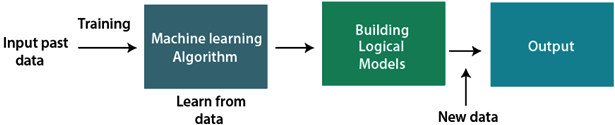
\includegraphics[width=0.73\linewidth]{images/intro/introduction-to-machine-learning.png}
		\end{figure}
	\end{block}
	
\end{frame}


\subsection[Contesto]{Contesto}
\begin{frame}
	%\frametitle{Definizione}
	
	\begin{block}{Contesto}
		Talvolta i due termini \textbf{Artificial Intelligence} (AI) e \mlbold (ML) vengono utilizzati erroneamente come sinonimi.\\
		Queste due tecnologie sono correlate tra loro, entrambe sono utilizzate per la creazione di sistemi intelligenti.\\
		Ad un livello più ampio, possiamo differenziare sia AI che ML in quanto:
		\begin{itemize}
			\item L'AI è un concetto più ampio per creare macchine intelligenti in grado di simulare capacità e comportamenti del pensiero umano,
			\item Mentre l'ML è un'applicazione o un sottoinsieme della AI che consente alle macchine di apprendere dai dati senza essere state programmato esplicitamente.
		\end{itemize}
	
	\end{block}
	
\end{frame}


\begin{frame}
	%\frametitle{Definizione}
		
	\begin{figure}[!htbp]
		\centering
		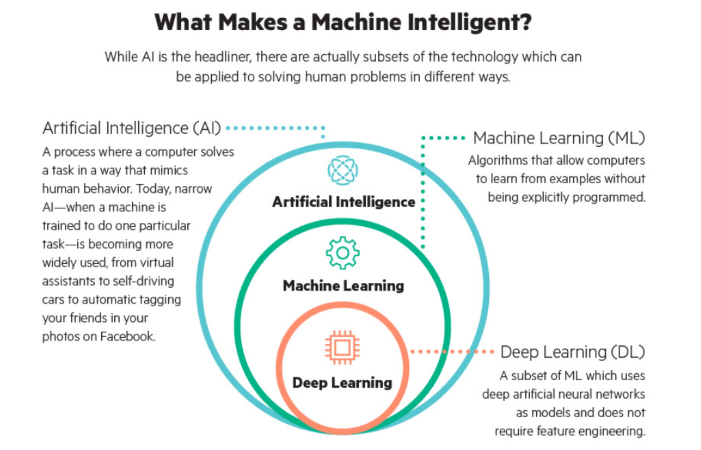
\includegraphics[width=12.0cm]{images/intro/ai_ml_dl.png}
	\end{figure}
	
\end{frame}


\subsection[Applicazioni]{Applicazioni}
\begin{frame}
	
	%\frametitle{1.0 Scopo}
	\begin{figure}[!htbp]
		\centering
		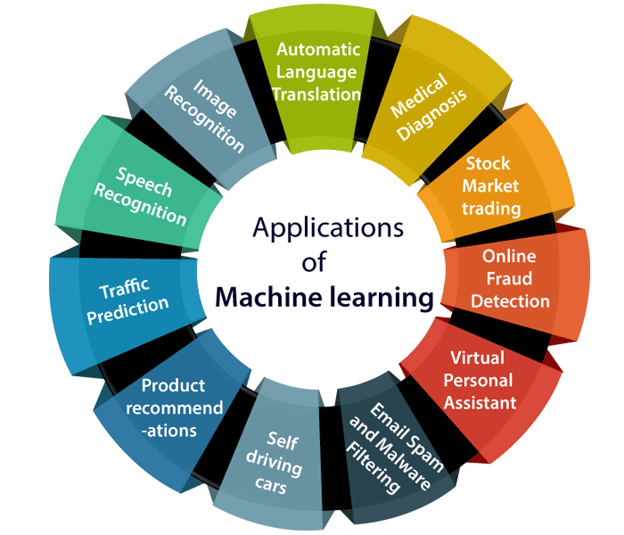
\includegraphics[width=9.0cm]{images/intro/ml_applications.png}
	\end{figure}

\end{frame}


\begin{frame}
	
	\frametitle{Applicazioni}
	%\begin{block}{}
		\begin{itemize}
			\item \textbf{Riconoscimento di immagini}:\\
				Il riconoscimento delle immagini è una delle applicazioni più comuni dell'apprendimento automatico. Viene utilizzato per identificare oggetti, persone, luoghi, immagini digitali, ecc\dots
			\begin{figure}[!htbp]
				\centering
				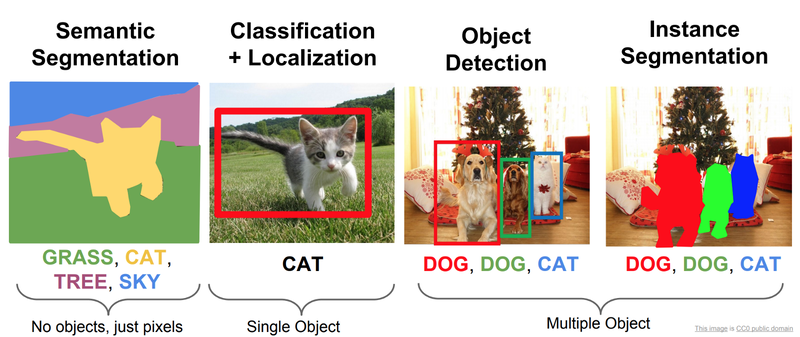
\includegraphics[width=11.0cm]{images/intro/ml_image_recognition.png}
			\end{figure}
			
		\end{itemize}		
	%\end{block}

\end{frame}

\begin{frame}
	
	\frametitle{Applicazioni}
	%\begin{block}{}
		\begin{itemize}
			\item \textbf{Riconoscimento vocale}:\\
				Il riconoscimento vocale è un processo di conversione delle istruzioni vocali in testo, spesso indicato come \textbf{Speech to Text} (STT) o \textbf{Computer Speech Recognition}. Al momento sono ampiamente utilizzati da varie applicazioni di riconoscimento vocale come:
				 	\begin{itemize}
				 		\item Google Assistant
				 		\item Siri
				 		\item Cortana
				 		\item Alexa
				 	\end{itemize}
			\begin{figure}[!htbp]
				\centering
				
\includegraphics[width=7.5cm]{images/intro/speech_recognition.png}
			\end{figure}
			
		\end{itemize}		
	%\end{block}

\end{frame}


\begin{frame}
	
	\frametitle{Applicazioni}
	%\begin{block}{}
		\begin{itemize}
			\item \textbf{Previsioni del traffico}:\\
				Se ci avvaliamo dell'aiuto di \textit{Tom Tom} o \textit{Google Maps} per visitare un luogo, ci viene indicato il percorso più breve con una indicazione circa le condizioni del traffico. 
				Riescono a predire se il traffico è assente, presente o fortemente congestionato con l'aiuto di informazioni incrociate: 
				\begin{itemize}
				 		\item la posizione in tempo reale del veicolo (app + sensore gps)
				 		\item tempo medio di percorrenza dello stesso percorso negli ultimi giorni nella stessa fascia oraria
				 	\end{itemize}
				Tutti coloro che utilizzano questi servizi aiutano i providers a migliorare le proprie applicazioni.
				Prendono le informazioni dall'utente e le rimandano al rispettivo database per migliorarne le prestazioni.
				 	
			\begin{figure}[!htbp]
				\centering
				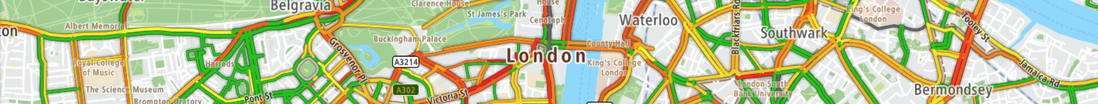
\includegraphics[width=10cm]{images/intro/tom_tom_traffic.png}
			\end{figure}
			
		\end{itemize}		
	%\end{block}

\end{frame}



\begin{frame}
	
	\frametitle{Applicazioni}
	%\begin{block}{}
		\begin{itemize}
			\item \textbf{Raccomandazioni}:\\
				Il ML è ampiamente utilizzato da varie società di e-commerce e intrattenimento come Amazon, Netflix, ecc \\
				per la raccomandazione di prodotti o film si cerca di comprendere gli interessi dell'utente utilizzando vari algoritmi di ML, quindi si tenta di suggerire un nuovo item sulla base di tali interessi.
				\begin{figure}[!htbp]
					\centering
					
\includegraphics[width=10.5cm]{images/intro/recommendations_examples.png}
				\end{figure}
		\end{itemize}		
	%\end{block}

\end{frame}


\begin{frame}
	
	\frametitle{Applicazioni}
	%\begin{block}{}
		\begin{itemize}
			\item \textbf{Auto a guida autonoma}:\\
				Una delle applicazioni più interessanti dell'apprendimento automatico sono le auto a guida autonoma.\\
				%Tesla, la più famosa azienda produttrice di auto, sta lavorando su auto a guida autonoma. Utilizza un metodo di apprendimento senza supervisione per addestrare i modelli di auto a rilevare persone e oggetti durante la guida.
				
				\begin{columns}
							
					\column{0.5\linewidth}
					\begin{figure}[!htbp]
						\centering
						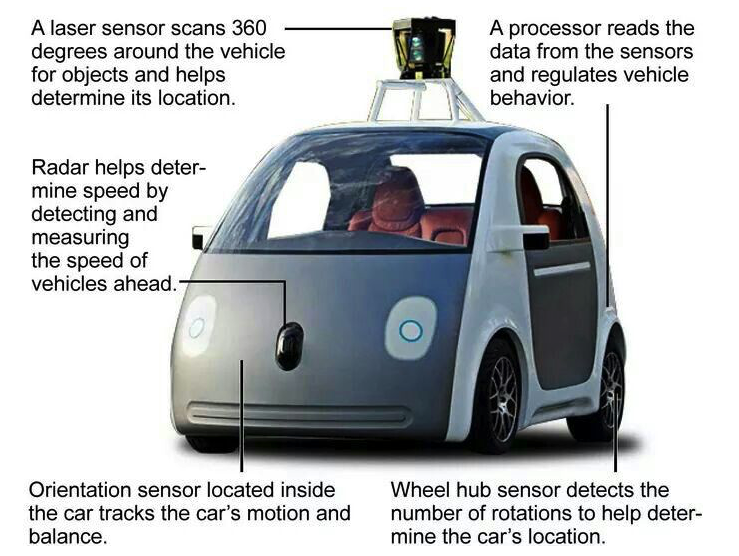
\includegraphics[angle=0,width=\linewidth]{images/intro/self_driving_car_google.jpg}
						\caption{Google Self Driving Car}
						%\label{Enel_HistFit_Normal} 
					\end{figure}
								
					\column{0.5\linewidth}
					\begin{figure}[!htbp]
						\centering
						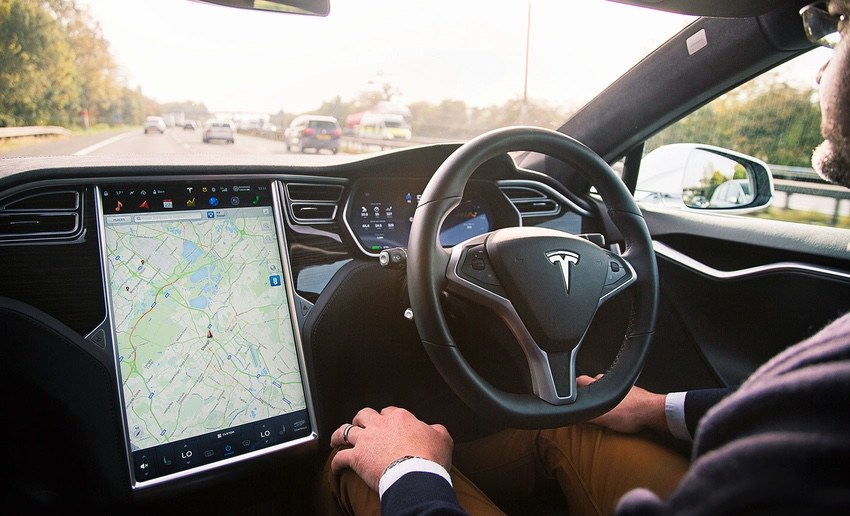
\includegraphics[angle=0,width=\linewidth]{images/intro/self_driving_car_tesla_autopilot.jpg}
						\caption{Tesla Auto Pilot}
						%\label{Enel_QQ_Plot_Normal} 
					\end{figure}
							
				\end{columns}

		\end{itemize}		
	%\end{block}

\end{frame}

\begin{frame}
	\frametitle{Applicazioni}
	%\begin{block}{}
		\begin{itemize}
			\item \textbf{Filtro antispam e malware per e-mail}:\\
				Ogni volta che riceviamo una nuova e-mail, viene automaticamente filtrata come importante, normale o spam. La posta elettronica è un modo efficiente per scambiare informazioni. Considerando la crescita di Internet e l'ampio utilizzo della posta elettronica, il tasso di aumento dello spam è motivo di grande preoccupazione.
				\begin{figure}[!htbp]
					\centering
					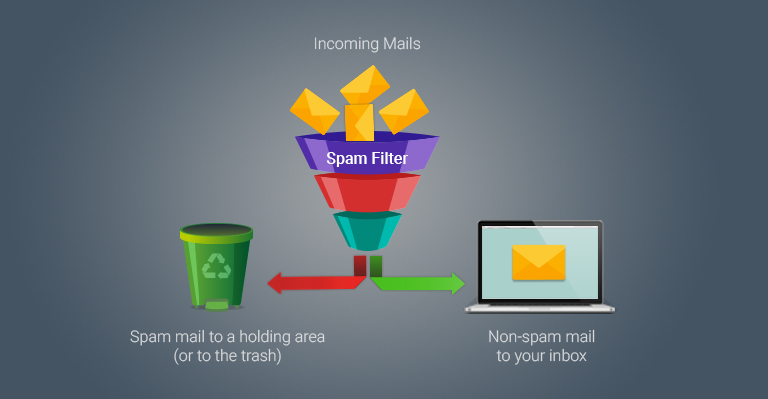
\includegraphics[width=7.5cm]{images/intro/anti-spam-filtering-techniques.jpg}
				\end{figure}
		\end{itemize}		
	%\end{block}
\end{frame}


\begin{frame}
	\frametitle{Applicazioni}
	%\begin{block}{}
		\begin{itemize}
			\item \textbf{Virtual Personal Assistant}:\\
				Esistono vari assistenti personali virtuali come Google Assistant, Alexa, Cortana, Siri, etc...\\
				Semplicemente con le nostre istruzioni vocali possiamo ordinare a questi dispositivi di riprodurre musica, chiamare qualcuno, aprire un'email, pianificare un appuntamento, ed altro.
				% Registrano le nostre istruzioni vocali, le inviano tramite su un servizio cloud dove vengono decodificate utilizzando algoritmi ML ed infine agiscono di conseguenza.
				\begin{figure}[!htbp]
					\centering
					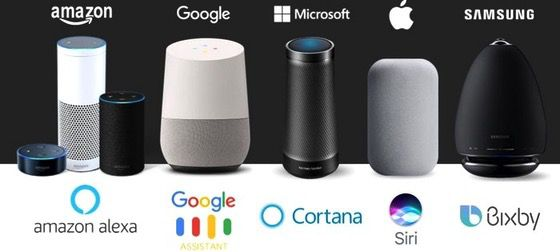
\includegraphics[width=8.5cm]{images/intro/assistants-vocaux.jpg}
				\end{figure}
		\end{itemize}		
	%\end{block}
\end{frame}


\begin{frame}
	\frametitle{Applicazioni}
	%\begin{block}{}
		\begin{itemize}
			\item \textbf{Rilevamento di frodi online}:\\
				Il ML sta rendendo le transazioni online più sicure e protette rilevando le transazioni fraudolente. Ogni volta che eseguiamo una transazione online, ci possono essere vari modi in cui può avvenire una transazione fraudolenta come account falsi, ID falsi o a metà di una transazione.
				%Quindi, per rilevarlo, possiamo avvalerci di questi strumenti che ci permettono di verificare se si tratta di una transazione autentica o di una transazione fraudolenta.\\
				
				\begin{figure}[!htbp]
					\centering
					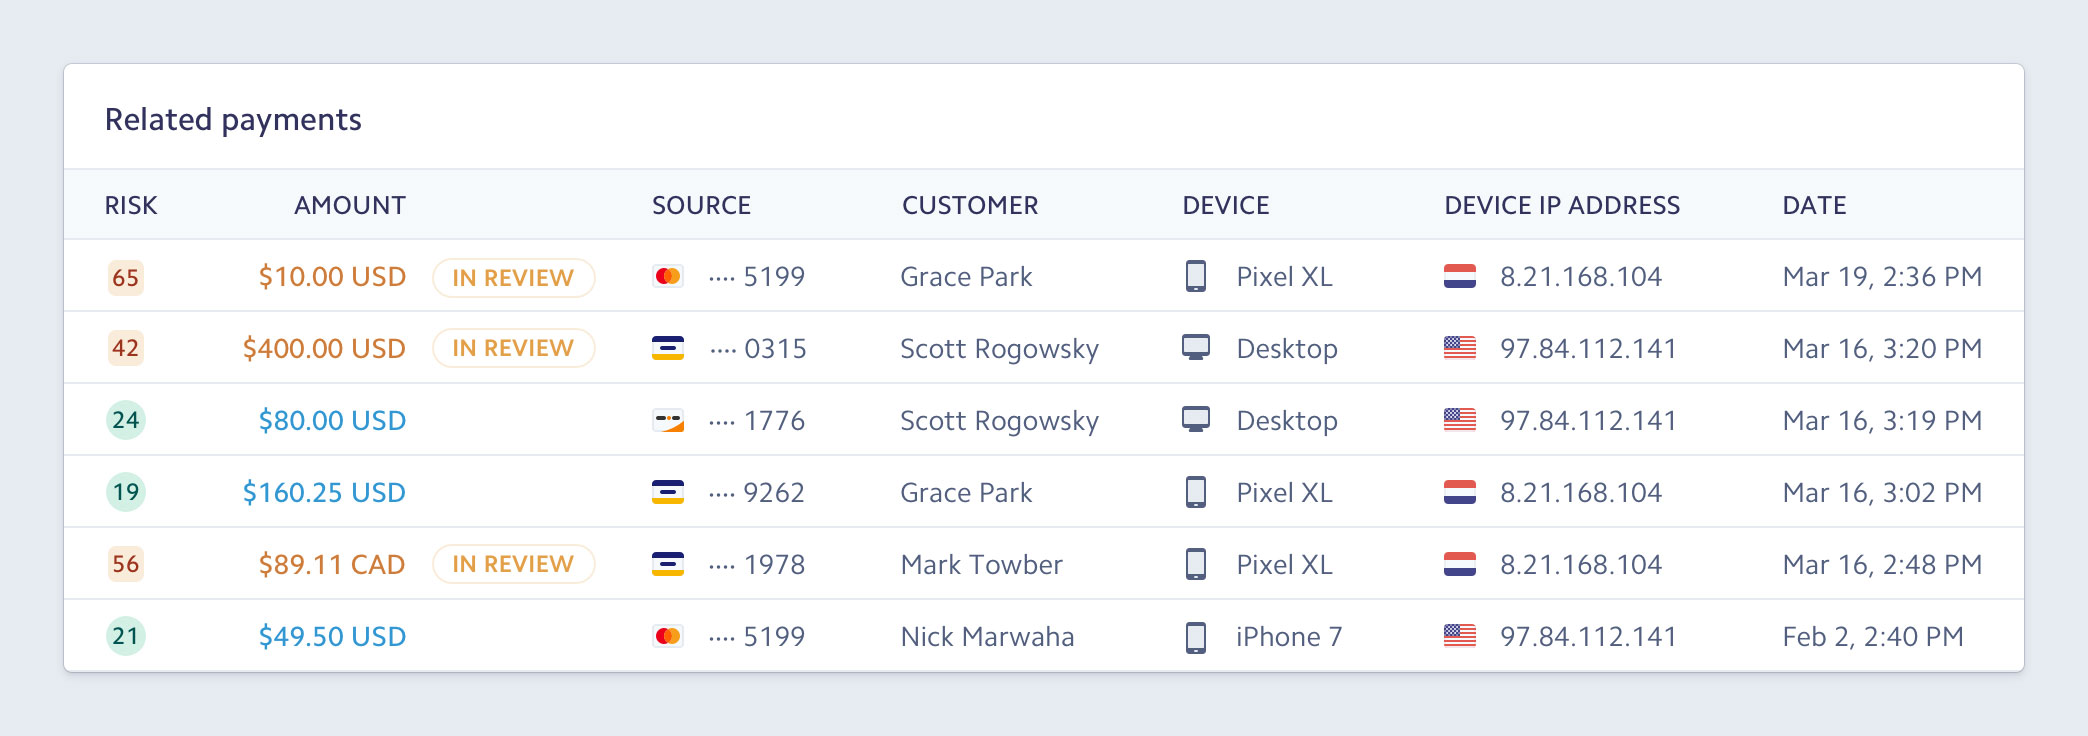
\includegraphics[width=9.5cm]{images/intro/stripe_radar.jpg}
					\caption{Stripe Radar for Fraud Detection}
				\end{figure}
		\end{itemize}		
	%\end{block}
\end{frame}



\begin{frame}
	\frametitle{Applicazioni}
	%\begin{block}{}
		\begin{itemize}
			\item \textbf{Trading}:\\
				L'apprendimento automatico è ampiamente utilizzato nel trading in borsa.\\
				Nel mercato azionario i prezzi delle azioni sono in continuo movimento.\\
				Il ML viene utilizzato per prevedere possibili trend di mercato oppure all'interno di trading systems automatici per generare ordini di compravendita automatici.
				\begin{figure}[!htbp]
					\centering
					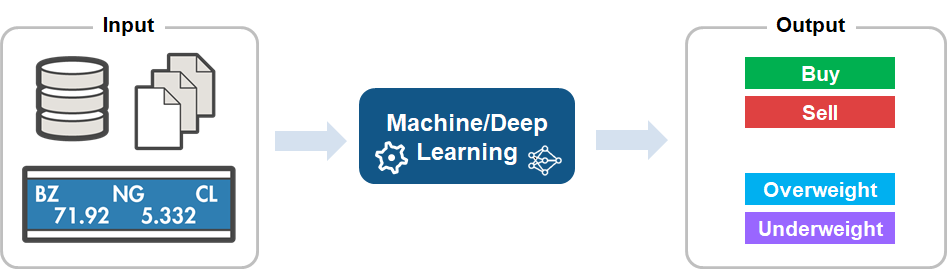
\includegraphics[width=10.5cm]{images/intro/ml_in_trading.png}
					%\caption{Stripe Radar for Fraud Detection}
				\end{figure}
		\end{itemize}		
	%\end{block}
\end{frame}


\begin{frame}
	\frametitle{Applicazioni}
	%\begin{block}{}
		\begin{itemize}
			\item \textbf{Diagnosi medica}:\\
				Nella scienza medica, il ML viene utilizzato per la diagnosi di alcune malattie.\\
				La tecnologia medica sta crescendo molto velocemente ed è ora in grado di costruire modelli 3D in grado ad esempio di localizzare l'esatta posizione di lesioni nel cervello (ad esempio tumori celebrali o altre malattie correlate al cervello).
				\begin{figure}[!htbp]
					\centering
					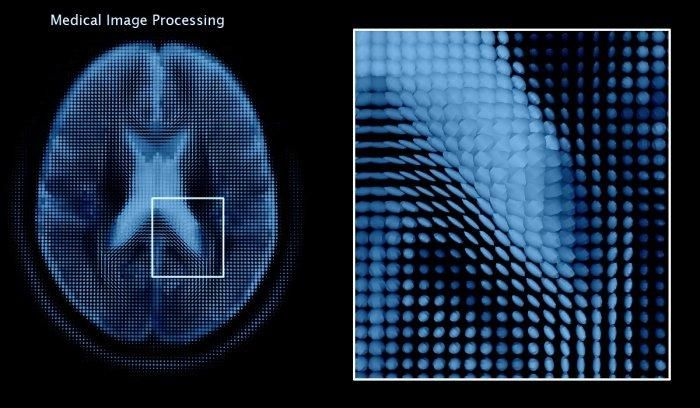
\includegraphics[width=5.7cm]{images/intro/medical_image_processing.jpg}
					%\caption{Stripe Radar for Fraud Detection}
				\end{figure}
		\end{itemize}		
	%\end{block}
\end{frame}


\begin{frame}
	\frametitle{Applicazioni}
	%\begin{block}{}
		\begin{itemize}
			\item \textbf{Traduzioni automatiche}:\\
				Al giorno d'oggi, se visitiamo un posto nuovo e non siamo a conoscenza della lingua allora non è affatto un problema.\\
				Ad esempio il GNMT di Google (Google Neural Machine Translation) fornisce questa funzionalità, traduce il testo nella nostra lingua.
				
				\begin{columns}
							
					\column{0.5\linewidth}
					\begin{figure}[!htbp]
						\centering
						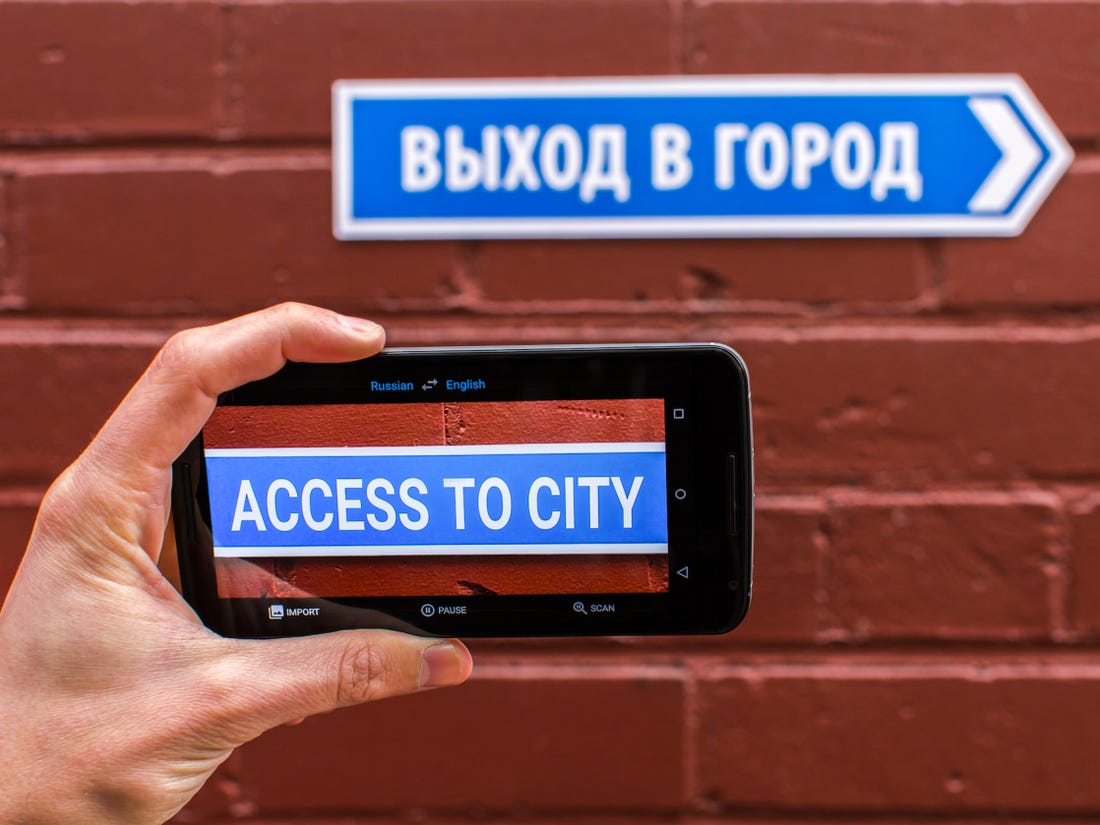
\includegraphics[angle=0,width=\linewidth]{images/intro/ml_gtranslate_1.jpeg}
						%\caption{Google Self Driving Car}
						%\label{Enel_HistFit_Normal} 
					\end{figure}
								
					\column{0.5\linewidth}
					\begin{figure}[!htbp]
						\centering
						
\includegraphics[angle=0,width=\linewidth]{images/intro/ml_gtranslate_2.jpeg}
						%\caption{Tesla Auto Pilot}
						%\label{Enel_QQ_Plot_Normal} 
					\end{figure}
							
				\end{columns}
			\end{itemize}		
	%\end{block}
\end{frame}


\begin{frame}
	
	%\frametitle{1.0 Scopo}
	\begin{figure}[!htbp]
		\centering
		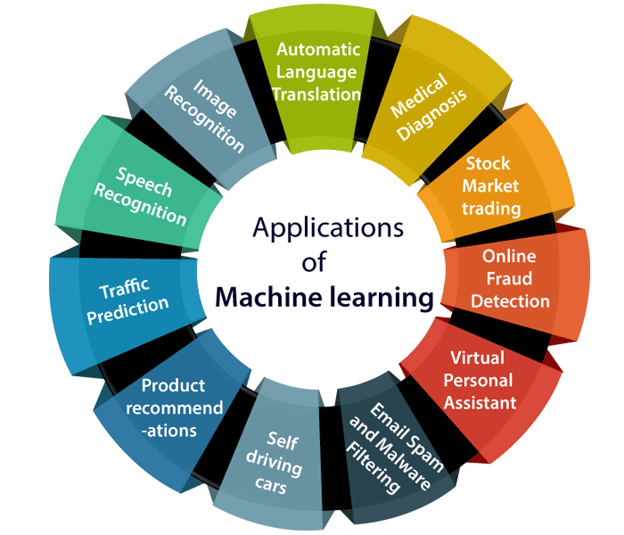
\includegraphics[width=9.0cm]{images/intro/ml_applications.png}
	\end{figure}

\end{frame}
\section[Glossario]{Glossario}
\sectionframe{images/covers/cover_glossary.jpg}{Glossario}


% Ottavio Calzone: Pagina 36-72 tipologie di apprendimento
\subsection[Machine learning, Statistical learning, \& Co.]{Machine learning, Statistical learning, \& Co.}


% TODO rivedere questa slide
\begin{frame}
	%\frametitle{Definizione}

	\begin{block}{Machine learning, Statistical learning, \& Co.}
		L'ambito di ricerca che affronta questa tipologia di problemi ha nomi diversi: Machine Learning (ML), Statistical Learning (SL), Data mining, Data science, Big data, ...\\
		In gran parte questi campi sono sovrapposti.\\
		Tuttavia esistono alcune differenze:
		\begin{itemize}
			\item alcune di queste discipline sono nate in dipartimenti di informatica, altre in quelli di statistica
			\item alcune applicazioni tendono a considerare campioni con dimensioni diverse, e sono meno interessate all'interpretabilità del risultato finale
			\item alcune si concentrano maggiormente su ciò che misuriamo, altre seguono semplicemente la logica che ciò che funziona anche vero
			\item Soprattutto: esistono differenze terminologiche (vedi slide seguente)
			\item ma queste discipline interagiscono e collaborano fra loro (in maniera competitiva...)
		\end{itemize}
	\end{block}

\end{frame}


\subsection[Il glossario di Tibshirani]{Il glossario di Tibshirani}
\begin{frame}

	\frametitle{Il glossario di Tibshirani}

	%\begin{block}{}
		Nel suo corso di statistica, \textbf{Rob Tibshirani}, uno statistico che si è applicato in parte anche nel ML, fornisce un \textbf{glossario} che mappa\\
		i termini del machine learning nei termini statistici:
		\begin{figure}[!htbp]
			\centering
			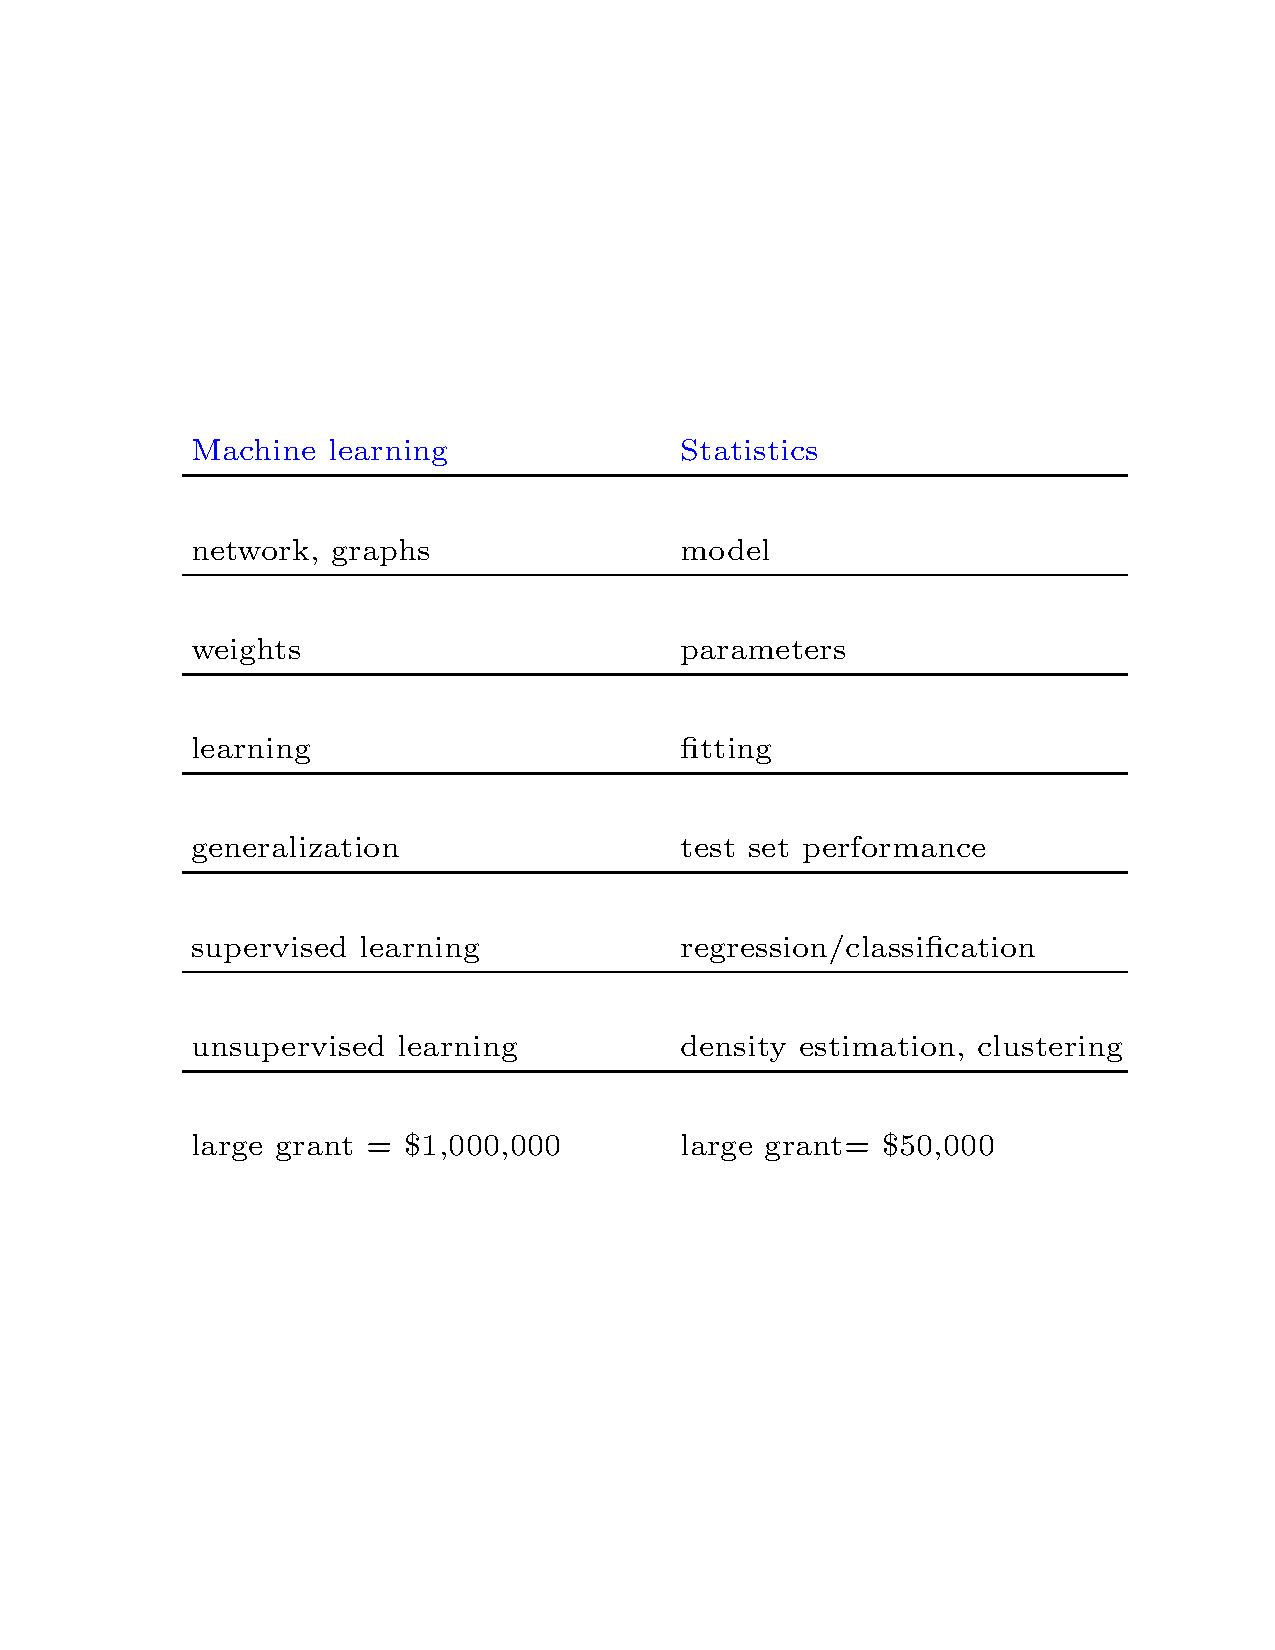
\includegraphics[width=6.5cm]{images/glossary/tibshirani_glossary.pdf}
			%\caption{Stripe Radar for Fraud Detection}
		\end{figure}
	%\end{block}


\end{frame}


\begin{frame}

	% Il \ml è Computational Applied Statistics
	\begin{block}{Come funziona il Machine Learning?}
		Dal momento che il ML considera il \textbf{mondo} stesso \textbf{rappresentabile} come \textbf{formule matematiche e statistiche}, i suoi algoritmi tentano di conoscere meglio tali formule inferendole da un numero di osservazioni limitato.
		\newlinedouble
		Come per un essere umano, non è necessario vedere prima tutti gli alberi che esistono nel mondo per riconoscerne uno (dal momento che gli esseri umani sono in grado di imparare quali sono le loro caratteristiche distintive); allo stesso modo, basandosi unicamente su un numero finito di esempi, gli algoritmi di machine learning possono usare la potenza di calcolo dei computer e l'abbondanza di dati, riguardanti praticamente qualsiasi argomento, per imparare a risolvere un enorme numero di problemi importanti e la cui soluzione riveste una notevole utilità per tutti noi.
		 \vskip5mm
		\hspace*\fill{\small--- \textit{Machine Learning for Dummies - Massaron e Mueller} }
	\end{block}


\end{frame}


\subsection[Features]{Features}
\begin{frame}

	\frametitle{Glossario}
	\framesubtitle{introduciamo alcuni termini ricorrenti nel \ml}

	\begin{block}{Features}
		Una \textbf{feature} (in italiano  \textbf{caratteristica}) è una variabile di input,\\
		ad esempio la variabile $\textbf{x}$ nella regressione lineare semplice.\\
		\vspace{1.8mm}
		Un progetto semplice potrebbe utilizzare anche una singola \textbf{feature}, mentre un progetto più complesso potrebbe utilizzare anche milioni di \textbf{features}, specificate come:\\
  			\makebox[\textwidth]{$\textbf{x}_{\textbf{1}}, \textbf{x}_{\textbf{2}},..., \textbf{x}_{\textbf{N}}$}\\
		\vspace{1.8mm}
		\pause
		Nell'esempio del rilevatore di spam, le \textbf{features} potrebbero includere:
		\begin{itemize}
			\pause
			\item il numero di parole nel testo dell'email
			\pause
			\item l'indirizzo del mittente
			\pause
			\item l'ora del giorno in cui è stata inviata l'email
			\pause
			\item l'email contiene la frase ``one weird trick''.
		\end{itemize}

	\end{block}

\end{frame}


\begin{frame}

	\frametitle{Glossario}
	\framesubtitle{introduciamo alcuni termini ricorrenti nel \ml}

	\begin{block}{}
		Le \textbf{features} possono essere:
		\begin{itemize}
			\item \textbf{quantitative}: valori numerici, rappresentanti misure
			\item \textbf{qualitative}: dette anche \textbf{categoriche/discrete/fattori}:\\
				stringhe di testo rappresentanti delle qualità
		\end{itemize}
		\pause
		
		\begin{columns}
			\column{0.55\linewidth}
			
			\begin{figure}[!htbp]
				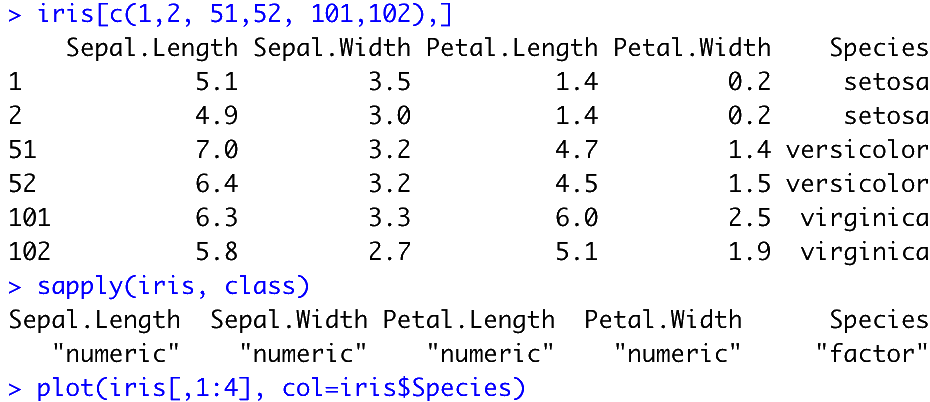
\includegraphics[width=1.0\linewidth]{images/glossary/iris_1.png}
				%\caption{}
			\end{figure}
			
%			\column{0.45\linewidth}
%			\begin{figure}[!htbp]
%				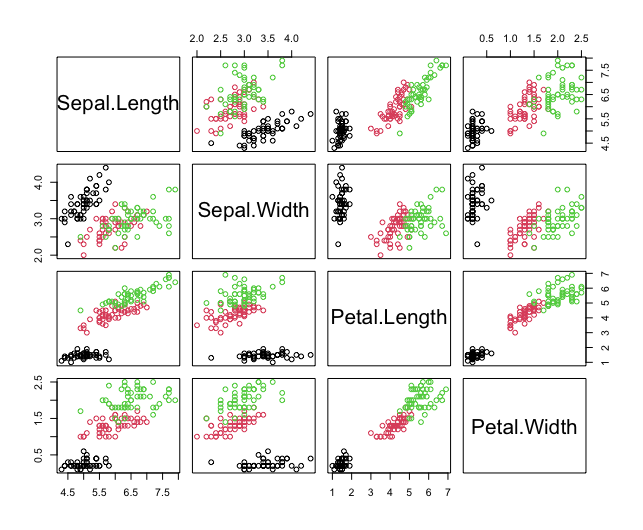
\includegraphics[width=1.0\linewidth]{images/glossary/iris_2.png}
%				%\caption{}
%			\end{figure}
		\end{columns}
		
	\end{block}

\end{frame}





\begin{frame}

	\frametitle{Glossario}
	\framesubtitle{introduciamo alcuni termini ricorrenti nel \ml}
	
		\href{https://en.wikipedia.org/wiki/Iris_flower_data_set}{\underline{\textbf{Iris Flower Data Set}}}: esempio di estrazione di features quantitative		
		
		\begin{figure}[!htbp]
			\centering
				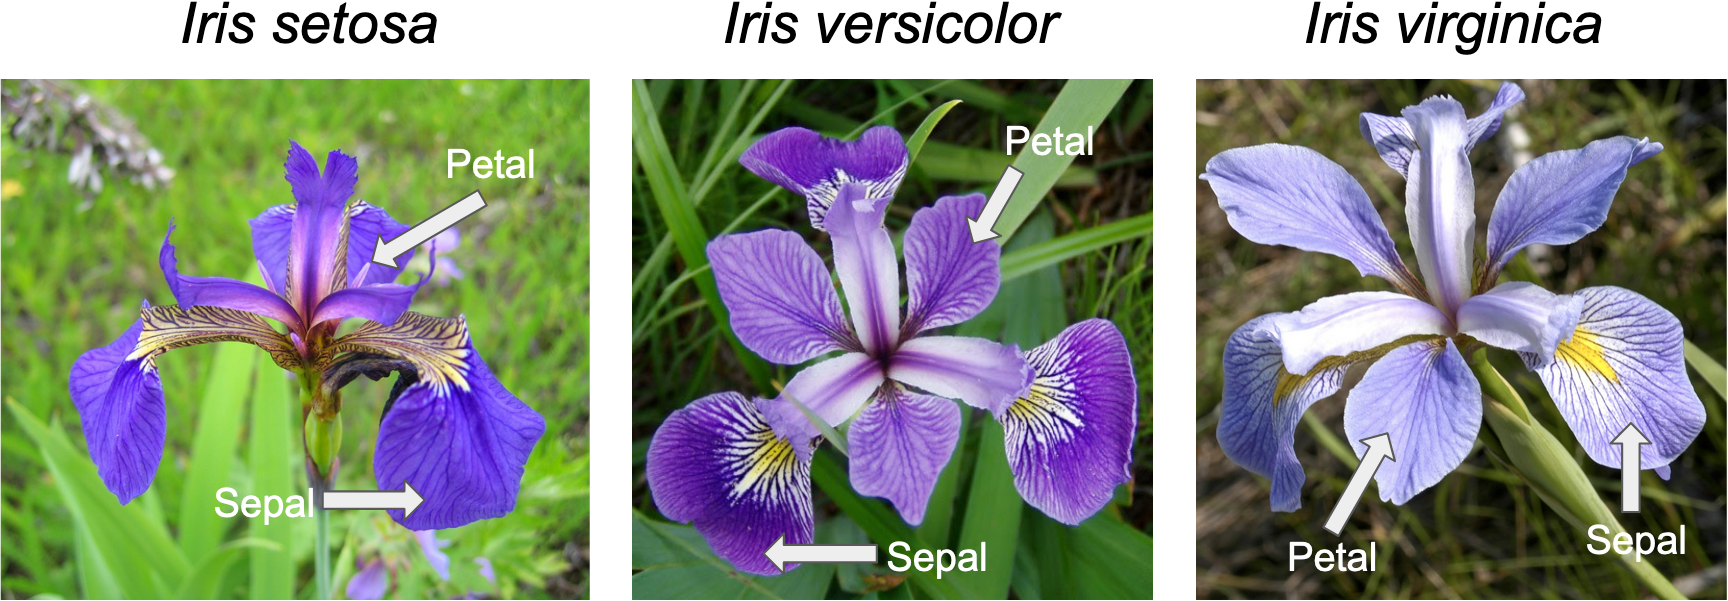
\includegraphics[width=0.75\linewidth]{images/glossary/iris_petal_sepal.png}
				%\caption{Stripe Radar for Fraud Detection}
			\end{figure}
		\pause
		
		\begin{columns}
			\column{0.4\linewidth}
			
			\begin{figure}[!htbp]
				\hspace{15mm}
				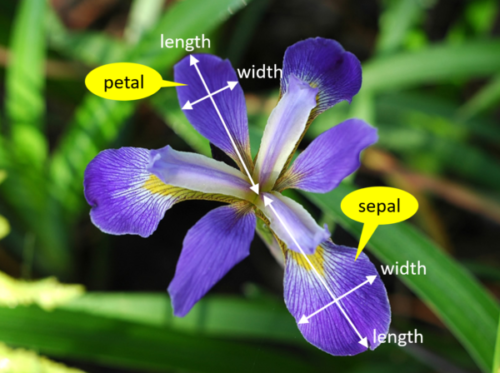
\includegraphics[width=0.65\linewidth]{images/glossary/iris_petal_sepal_features.png}
				
				%\caption{}
			\end{figure}
			
			\pause
			\column{0.01\linewidth}
			\begin{large}
				\vspace{5mm}
				$$\pmb{\Rightarrow}$$
			\end{large}
			
			\column{0.59\linewidth}
			\begin{figure}[!htbp]
				\centering
				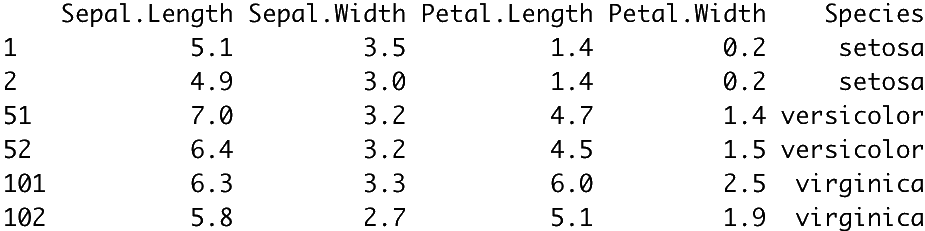
\includegraphics[width=0.85\linewidth]{images/glossary/iris_3.png}
				%\caption{}
			\end{figure}	
		\end{columns}


\end{frame}





\subsection[Labels]{Labels}
\begin{frame}

	\frametitle{Glossario}
	\framesubtitle{introduciamo alcuni termini ricorrenti nel \ml}

	\begin{block}{Labels}
		Una \textbf{label} o \textbf{classe} è ciò vogliamo predire con il nostro modello di ML:\\
		ad esempio la variabile $y$ nella regressione lineare semplice.
		\newlinedouble
		\pause
		Una \textbf{label} potrebbe essere:
		\begin{itemize}
			\pause
			\item spam oppure non spam
			\pause
			\item la tipologia di iris: setosa, versicolor o virginica
			\pause
			\item il tipo di animale mostrato in un'immagine
			\pause
			\item il prezzo futuro del grano
			\pause
			\item la temperatura esterna
			\pause
			\item ...
		\end{itemize}
	\end{block}

\end{frame}


\begin{frame}

	\frametitle{Glossario}
	\framesubtitle{introduciamo alcuni termini ricorrenti nel \ml}

	\begin{figure}[!htbp]
		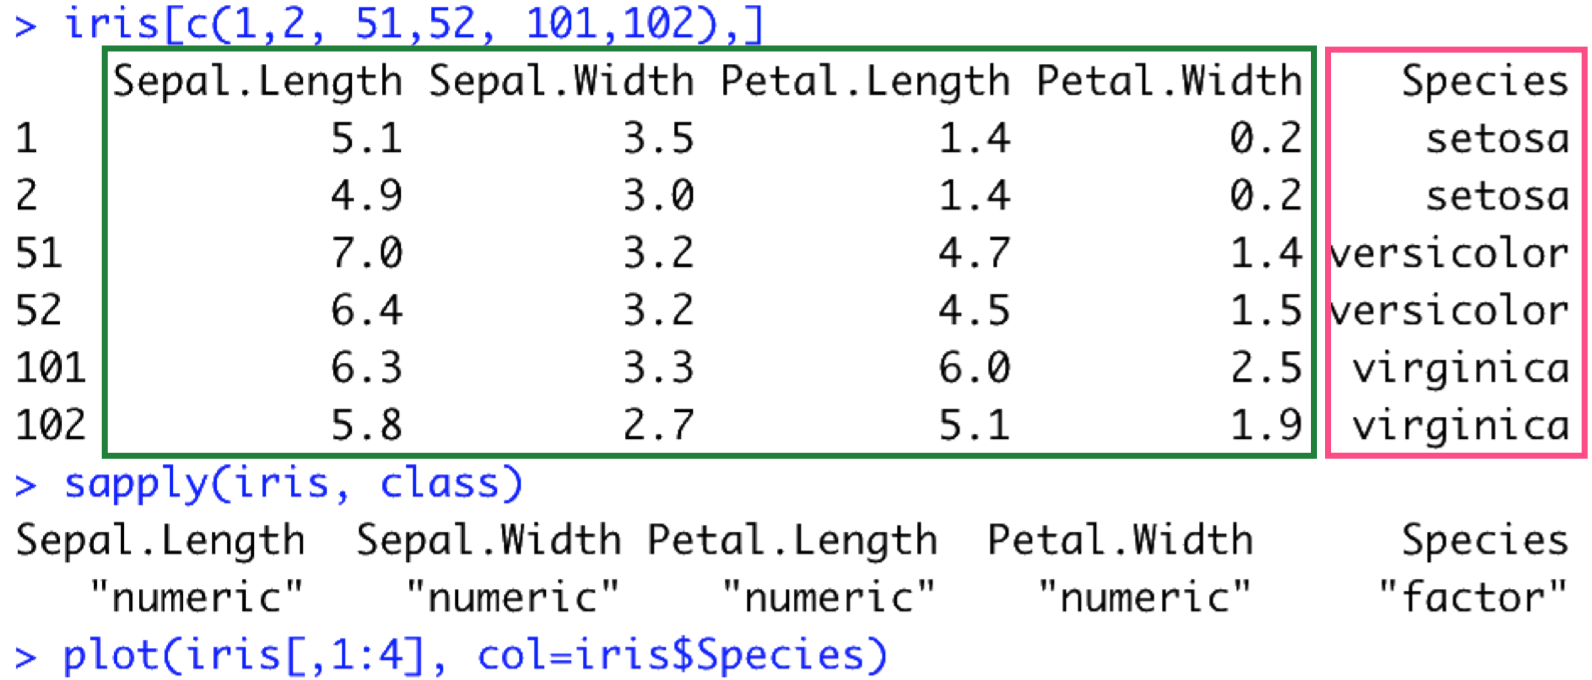
\includegraphics[width=1.0\linewidth]{images/glossary/iris_4.png}
		%\caption{}
	\end{figure}


\end{frame}



\subsection[Examples]{Examples}
\begin{frame}

	\frametitle{Glossario}
	\framesubtitle{introduciamo alcuni termini ricorrenti nel \ml}

	\begin{block}{Examples}
		Un \textbf{esempio} (example) è una particolare istanza di dati, \textbf{x}\\
		(mettiamo x in grassetto per indicare che si tratta di un vettore).
		\newlinedouble
		Dividiamo gli \textbf{esempi} in due categorie:
		\begin{itemize}
			\item esempi etichettati (labeled examples)
			\item esempi non etichettati (unlabeled examples)
		\end{itemize}

	\end{block}

\end{frame}


\subsubsection[Labeled Examples]{Labeled Examples}
\begin{frame}

	\frametitle{Glossario}
	\framesubtitle{introduciamo alcuni termini ricorrenti nel \ml}

	\begin{block}{Labeled Examples}
		Un \textbf{labeled example} (esempio etichettato)\\
		include sia la(le) caratteristica(e) che l'etichetta,\\
		ovvero:
		\newlinedouble
		\makebox[\textwidth]{\textbf{labeled examples: \{features, label\}: (x, y)}}
		\newlinedouble

		Nel nostro esempio del rilevamento dello spam, gli esempi etichettati sarebbero singole email che gli utenti hanno esplicitamente contrassegnato come ``spam'' o ``non spam''.

	\end{block}

\end{frame}


\begin{frame}

	\frametitle{Glossario}
	\framesubtitle{introduciamo alcuni termini ricorrenti nel \ml}

	\begin{block}{Labeled Examples}
		Ad esempio, la seguente tabella mostra 5 \textbf{esempi etichettati} presi da un dataset contenente informazioni sui prezzi delle case in California:
		\newlinedouble

	% Text size https://texblog.org/2012/08/29/changing-the-font-size-in-latex/
	\begin{scriptsize}
		\begin{table}
		\begin{tabular}{|c|c|c|c|}
		\hline
		\rowcolor{gray!25} \textbf{housingMedianAge} & \textbf{totalRooms} & \textbf{totalBedrooms} & \textbf{medianHouseValue} \\
		\rowcolor{gray!25} \textbf{(feature)} & \textbf{(feature)} & \textbf{(feature)} & \textbf{(label)} \\ \hline
		\textit{15} & \textit{5612} & \textit{1283} & \cellcolor{yellow!15} \textit{66900} \\ \hline
		\textit{19} & \textit{7650} & \textit{1901} & \cellcolor{yellow!15}\textit{80100} \\ \hline
		\textit{17} & \textit{720} & \textit{174} & \cellcolor{yellow!15}\textit{85700} \\ \hline
		\textit{14} & \textit{1501} & \textit{337} & \cellcolor{yellow!15}\textit{73400} \\ \hline
		\textit{20} & \textit{1454} & \textit{326} & \cellcolor{yellow!15}\textit{65500} \\ \hline
		\end{tabular}
		\end{table}
	\end{scriptsize}

	\end{block}

\end{frame}


\subsubsection[Unlabeled Examples]{Unlabeled Examples}
\begin{frame}

	\frametitle{Glossario}
	\framesubtitle{introduciamo alcuni termini ricorrenti nel \ml}

	\begin{block}{Unlabeled Examples}
		Un \textbf{unlabeled example} (esempio non etichettato)\\
		contiene la(le) caratteristica(e) ma non l'etichetta,\\
		ovvero:
		\newlinedouble
		\makebox[\textwidth]{\textbf{unlabeled examples: \{features, ?\}: (x, ?)}}

	\end{block}

\end{frame}



\begin{frame}

	\frametitle{Glossario}
	\framesubtitle{introduciamo alcuni termini ricorrenti nel \ml}

	\begin{block}{Unlabeled Examples}
		Di seguito sono riportati 3 \textbf{esempi senza etichetta} dello stesso dataset riguardante le case in California, che escludono \textbf{medianHouseValue}:

			% Text size https://texblog.org/2012/08/29/changing-the-font-size-in-latex/
		\begin{scriptsize}
			\begin{table}
			\begin{tabular}{|c|c|c|c|}
			\hline
			\rowcolor{gray!25} \textbf{housingMedianAge} & \textbf{totalRooms} & \textbf{totalBedrooms} & \textbf{medianHouseValue} \\
			\rowcolor{gray!25} \textbf{(feature)} & \textbf{(feature)} & \textbf{(feature)} & \textbf{(label)} \\ \hline
			\textit{42} & \textit{1686} & \textit{361} & \cellcolor{yellow!15}\textit{?} \\ \hline
			\textit{34} & \textit{1226} & \textit{180} & \cellcolor{yellow!15}\textit{?} \\ \hline
			\textit{33} & \textit{1077} & \textit{271} & \cellcolor{yellow!15}\textit{?} \\ \hline
			\end{tabular}
			\end{table}
		\end{scriptsize}

		Dopo aver addestrato il nostro modello con esempi etichettati, utilizziamo quel modello per prevedere l'etichetta su esempi senza etichetta.
		\newlinedouble
		Nel rilevatore di spam, esempi senza etichetta sono le nuove e-mail che gli esseri umani non hanno ancora etichettato (come ``spam'' o ``non spam'').
	\end{block}

\end{frame}


\subsection[Funzione target]{Funzione target}
% TODO Rileggere: funzione target...
\begin{frame}

	\frametitle{Glossario}
	\framesubtitle{introduciamo alcuni termini ricorrenti nel \ml}

	\begin{block}{Funzione target}

		Un bambino  astrae l’idea di come dovrebbe essere un albero confrontando le caratteristiche (feature) con le immagini di altri oggetti diversi.\\
		\vspace{2mm}
		 %, per esempio mobili che, pur essendo fatti di legno, non condividono con l’albero le altre caratteristiche.\\

		Un classificatore di machine learning funziona alla stessa maniera: le sue capacità cognitive vengono costituite sviluppando una formula matematica che comprenda tutte le feature fornite, in modo da arrivare ad avere una funzione che sia in grado di distinguere una classe dall’altra.\\
		\vspace{3mm}

		Supponiamo che esista una formula matematica, nota anche come \textbf{funzione target}, in grado di esprimere le caratteristiche di un albero.\\
		\vspace{2mm}
		Essere in grado di esprimere tale formula matematica costituisce quella che si chiama la \textbf{capacità rappresentativa} del classificatore.
	\end{block}

\end{frame}


\subsection[Ottimizzazione e spazio delle ipotesi]{Ottimizzazione e spazio delle ipotesi}
\begin{frame}

	\frametitle{Glossario}
	\framesubtitle{introduciamo alcuni termini ricorrenti nel \ml}

	\begin{block}{Ottimizzazione e spazio delle ipotesi}
		Durante l’\textbf{ottimizzazione} (il processo di calcolo dell’ottimizzatore), l’algoritmo svolge ricerche fra le possibili varianti delle combinazioni di parametri, per trovare quella migliore che consenta, nella fase di addestramento, una mappatura corretta tra le feature e le classi.\\
		\vspace{3mm}
		Questo processo calcola svariate possibili funzioni target fra quelle che l’algoritmo di apprendimento è in grado di scovare (\textbf{spazio delle ipotesi}).\\
		\vspace{3mm}
		Il classificatore risultante, unitamente a tutti i parametri impostati, prende il nome di \textbf{ipotesi}, che è un modo per dire, nel gergo del machine learning, che l’algoritmo ha impostato i parametri così da replicare la funzione target e ora è pronto a elaborare le classificazioni in modo corretto.
	\end{block}

\end{frame}


\subsection[Loss]{Loss}


\begin{frame}

	\frametitle{Glossario}
	\framesubtitle{introduciamo alcuni termini ricorrenti nel \ml}

	\begin{block}{Loss}
		Nel processo di ottimizzazione nel machine learning è la risposta da parte di una funzione interna all’algoritmo, chiamata \textbf{loss} (anche detta: \textit{funzione di costo}, \textit{funzione di perdita}, \textit{funzione obiettivo}, \textit{funzione di score} o \textit{funzione d’errore}), a giocare un ruolo di primo piano.\\
		\vspace{3mm}
		La \textbf{loss} è una funzione di valutazione che misura la capacità dell’algoritmo di machine learning di mappare la funzione target che sta cercando di individuare.\\
		\vspace{3mm}
		La \textbf{loss} opera mettendo a confronto le previsioni di un algoritmo con l’effettivo esito registrato nel mondo reale. Confrontare una previsione con il valore reale utilizzando una funzione di costo consente di stabilire il livello di errore dell’algoritmo.%\\
		%\vspace{3mm}
		%È la funzione di costo a stabilire il successo di un’applicazione di machine learning: per quanto riguarda il processo di apprendimento, tale funzione è fondamentale tanto quanto la rappresentazione (che è la capacità di approssimare determinate funzioni matematiche) e l’ottimizzazione (il modo in cui gli algoritmi di machine learning impostano al meglio i propri parametri interni)
	\end{block}

\end{frame}


\subsection[Modello]{Modello}
\begin{frame}

	\frametitle{Glossario}
	\framesubtitle{introduciamo alcuni termini ricorrenti nel \ml}

	\begin{block}{Modello}
		Un \textbf{modello} definisce la relazione tra le features e la label.\\
		\vspace{2mm}
		%Ad esempio, un modello per il rilevamento dello spam potrebbe associare fortemente determinate feature allo ``spam''.\\
		%\vspace{2mm}
		Evidenziamo le due fasi della vita di un modello:
		\begin{itemize}
			\item \textbf{Training} significa creare o addestrare il modello.\\
					Ovvero, mostri al modello degli esempi etichettati e consenti al modello di apprendere gradualmente quale sia la relazione tra le caratteristiche e l'etichetta.
			\item \textbf{Inferenza} significa applicare il modello addestrato a esempi senza etichetta.\\
				Ovvero, si utilizza il modello addestrato per eseguire previsioni utili (\textbf{y'}). Ad esempio, applicando l'inferenza, è possibile prevedere medianHouseValue per nuovi esempi senza etichetta.
		\end{itemize}

	\end{block}

\end{frame}


\begin{frame}

	\frametitle{Glossario}
	\framesubtitle{introduciamo alcuni termini ricorrenti nel \ml}

	\begin{block}{Modello (il caso classico dell'apprendimento supervisionato)}
		\begin{figure}[!htbp]
			\centering
			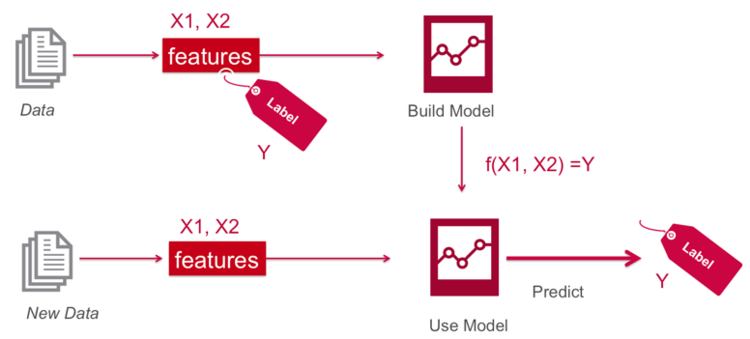
\includegraphics[width=11.9cm]{images/glossary/supervised_learning_1.png}
			%\caption{Stripe Radar for Fraud Detection}
			\label{fig:glossary_supervised_learning_1}
		\end{figure}

	\end{block}

\end{frame}


\begin{frame}

	\frametitle{Glossario}
	\framesubtitle{introduciamo alcuni termini ricorrenti nel \ml}

	\begin{block}{Modello (il caso classico dell'apprendimento supervisionato)}
		\begin{figure}[!htbp]
			\centering
			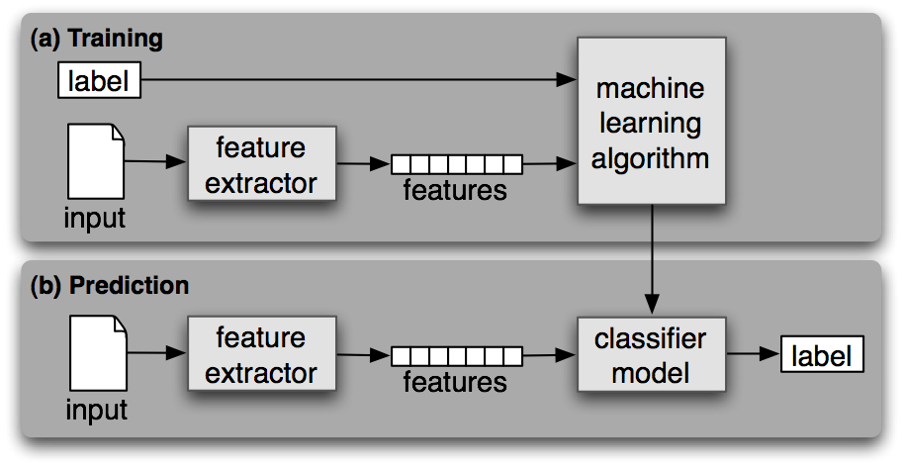
\includegraphics[width=11.2cm]{images/glossary/supervised_learning_2.png}
			\label{fig:glossary_supervised_learning_2}
			%\caption{Stripe Radar for Fraud Detection}
		\end{figure}

	\end{block}

\end{frame}


\ifthenelse{\boolean{highschool}}{}{
% https://medium.com/@dataakkadian/what-are-parametric-vs-nonparametric-models-8bfa20726f4d
\subsection[Modelli: parametrici vs non parametrici]{Modelli: parametrici vs non parametrici}

\begin{frame}

	\frametitle{Modelli: parametrici vs non parametrici}

	\begin{block}{Modelli: parametrici vs non parametrici}
		In base alle assunzioni che uno specifico modello stabilisce è possibile separare i modelli di machine learning in due categorie:
		\begin{itemize}
			\item modelli di tipo \textbf{parametrico}
			\item modelli di tipo \textbf{non parametrico}
		\end{itemize}
	\end{block}

\end{frame}


\subsubsection[Modelli Parametrici]{Modelli Parametrici}

\begin{frame}

	\frametitle{Modelli Parametrici}

	%\begin{block}{}
		\begin{itemize}
			\item riassumono i dati tramite un insieme finito di parametri $\theta$,\\
				indipendentemente dal numero di esempi di addestramento
			\item indipendentemente dalla quantità di dati forniti a un modello parametrico, questo non cambierà idea sul numero di parametri necessari per descrivere i dati
			\item quindi la complessità del modello è limitata anche se la quantità di dati è illimitata, questo li rende per certi versi \textbf{poco flessibili}
			\item i modelli parametrici asssumono una forma funzionale specifica per $f$, che dipende da un piccolo numero di $p$ \emph{parametri} ignoti:\\
				$$\theta = (\theta_1,\theta_2,\ldots,\theta_p)^\prime$$
			\item un modello parametrico può essere reso \emph{molto flessibile} aumentando il numero di parametri $p$
		\end{itemize}
	%\end{block}

\end{frame}





% TODO Valutare per caso mancasse un theta con 0 qui nel modello e nel predittore
\begin{frame}
	\frametitle{Modelli Parametrici}

	\begin{block}{Un esempio: la regressione lineare}
		\begin{itemize}
		\item esempio: Regressione lineare\\
	  			\makebox[\textwidth]{$f(X_i) = \theta_1 X_{i1}+\theta_2 X_{i2} + \ldots + \theta_p X_{ip}$}\\
			\vspace{2mm}
			\item usiamo il campione per \emph{stimare} $\theta$ o \emph{addestrare (fit/train)} il modello. Di solito per farlo ottimizziamo una misura dell'adattamento ai dati
			\item esempio: Minimi quadrati $\widehat\theta = (\mbX^\prime \mbX)^{-1} \mbX' \bfy = \mbX^{+}\bfy$\\
			(un metodo di stima \emph{globale}, dove $X^{+}$ è la matrice pseudoinversa di Moore-Penrose di $X$)
		\item Il \emph{predittore} è dato da
			$$\widehat{f}(X_0) = \widehat{\theta}_1 X_{i1} + \widehat{\theta}_2 X_{i2} + \ldots + \widehat{\theta}_p X_{ip}$$
		\end{itemize}
	\end{block}
\end{frame}


\subsubsection[Modelli Non Parametrici]{Modelli Non Parametrici}

\begin{frame}

	\frametitle{Modelli Non Parametrici}

	%\begin{block}{}
		\begin{itemize}
			\item non richiedono una ipotesi sulla forma di $f$
			\item sono utili quando si hanno molti dati e nessuna conoscenza precedente e quando non ci si vuole preoccupare troppo di scegliere le features giuste
			\item presuppongono che la distribuzione dei dati non possa essere definita in termini di un insieme finito di parametri.\\
				Ma spesso possono essere definiti assumendo un $\theta$ di dimensione infinita. Solitamente pensando a $\theta$ come ad una funzione
			\item la quantità di informazioni che $\theta$ può acquisire sui dati $D$ può aumentare al crescere della quantità di dati, questo li rende \textbf{più flessibili}
		\end{itemize}

	%\end{block}

\end{frame}


\subsubsection[Alcuni tradeoff]{Alcuni tradeoff}

\begin{frame}
	\frametitle{Alcuni tradeoff}
	\begin{itemize}
		\item Un modello parametrico può non essere abbastanza flessibile da adattarsi sufficientemente bene ai dati
		\item L'adattamento ai dati può essere migliorato usando un metodo più flessibile
		\item Ma questo non è sempre consigliabile
			\begin{enumerate}
				\item Un modello flessibile è più difficile da interpretare di un altro più semplice
					\begin{itemize}
						\item[--] i modelli lineari sono facili da interpretare, a differenza per es. di KNN
					\end{itemize}
				\item Un modello flessibile può adattarsi molto bene ai dati \emph{nel campione} ma prevedere molto male \emph{al di fuori di esso}; in altre parole può essere affetto da \emph{overfit}
					\begin{itemize}
						%\item notare che l'errore irriducibile $\Var(\varepsilon)$ non può essere ridotto
						\item[--] come possiamo sapere se l'adattamento ai dati nel campione di stima \`{e} adeguato?
					\end{itemize}
				\item Principio di parsimonia
					\begin{itemize}
						\item in generale, è sempre meglio preferire un modello con poche variabili rispetto a un predittore che ne usa molte in maniera non molto chiara e trasparente
					\end{itemize}
			\end{enumerate}
	\end{itemize}
\end{frame}


\begin{frame}

	\frametitle{Modelli: parametrici vs non parametrici}

	\begin{block}{Modelli: parametrici vs non parametrici}
		In conclusione con i modelli parametrici per effettuare delle nuove previsioni, è sufficiente conoscere i parametri del modello.
		\newlinedouble
		I metodi non parametrici sono più flessibili e per effettuare delle nuove previsioni è necessario conoscere i parametri del modello e lo stato dei dati che sono stati osservati.
	\end{block}

\end{frame}
}





\subsection[Tipi di apprendimento]{Tipi di apprendimento}
\begin{frame}

	\frametitle{Le tipologie di apprendimento}

	\begin{block}{Machine Learning, altre definizioni}
		$\Rightarrow$ computational statistics\\
		$\Rightarrow$ building computational artifacts that learn over time based on experience
	\end{block}

	\begin{block}{Le tipologie di apprendimento}

		Le tecniche di Machine Learning sono generalmente suddivise\\
		in tre grandi categorie:

		\begin{enumerate}
			\item ad apprendimento \textbf{non supervisionato} (unsupervised learning)
			\item ad apprendimento \textbf{supervisionato} (supervised learning)
			\item ad apprendimento \textbf{per rinforzo} (reinforcement learning)
		\end{enumerate}

		a seconda della natura del ``segnale'' utilizzato per l'apprendimento.
	\end{block}


\end{frame}


\begin{frame}

	\frametitle{Le tipologie di apprendimento}

	\begin{figure}[!htbp]
		\centering
		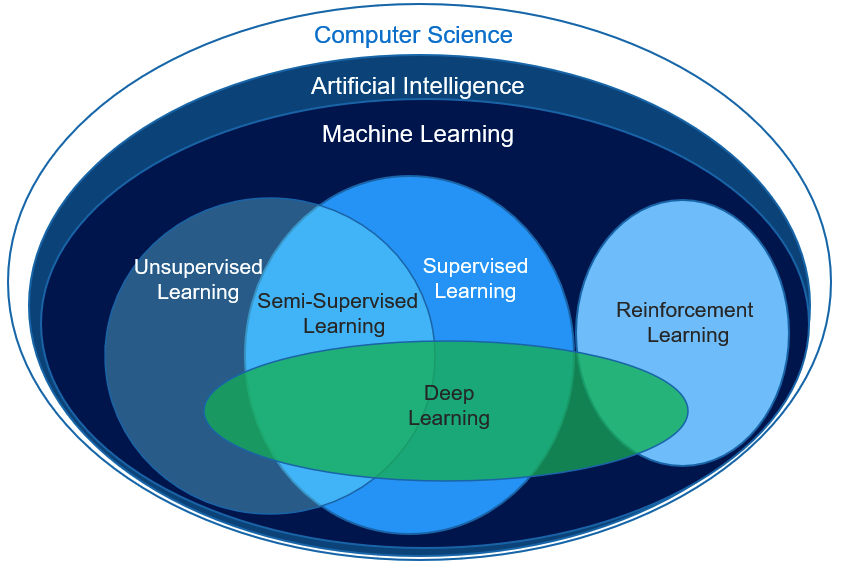
\includegraphics[width=10cm]{images/glossary/learning_types.png}
		%\caption{Stripe Radar for Fraud Detection}
	\end{figure}

\end{frame}


\subsubsection{Apprendimento non supervisionato}

\begin{frame}

	\frametitle{Apprendimento non supervisionato}

	\begin{block}{Qualche definizione}
		\begin{itemize}
			\item a partire da esempi non etichettati si cerca di derivare quali siano le caratteristiche che li accomunano/distinguono tra loro semplicemente osservando le relazioni che intercorrono tra gli esempi stessi
			\item questi algoritmi imparano semplicemente dagli esempi, senza che gli vengano fornite risposte associate (lables):\\
				è l'algoritmo stesso a stabilire autonomamente quali sono le caratteristiche distintive (i pattern) dei dati
			\item non vengono assegnate etichette all'algoritmo di apprendimento, lasciando che sia solo lui a trovare la struttura nel suo input.
			\item in breve ricavare una \textbf{descrizione compatta}
		\end{itemize}

	\end{block}


\end{frame}


\begin{frame}
	\frametitle{Apprendimento non supervisionato}
	\begin{block}{Osservazioni}
		\begin{itemize}
			\item può essere applicato come obiettivo in sè (osservare i dati sotto una diversa prospettiva, scoprendone nuovi significati; segmentare il mercato) o un mezzo per raggiungere un altro fine (creando nuovi input per gli algoritmi di machine learning supervisionati)
			\item si può fare un parallelo fra questi algoritmi e il modo in cui gli esseri umani cercano di comprendere che determinati oggetti o eventi appartengono alla stessa classe (effettuano associazioni sulla base del grado di somiglianza fra due oggetti)
			\item alcuni sistemi di raccomandazione presenti sul web vanno a ricercare possibili suggerimenti fra i dati relativi a ciò che avete acquistato in passato; le raccomandazioni sono basate sulla stima del gruppo di clienti a cui assomigliate di più, inferendo quindi le vostre probabili preferenze in base a tale gruppo
		\end{itemize}

	\end{block}

\end{frame}


\begin{frame}

	\frametitle{Apprendimento non supervisionato}

	\begin{block}{Un esempio di apprendimento non supervisionato: il clustering}
	
		
		\begin{columns}
			\column{0.425\linewidth}
			\begin{figure}[!htbp]
				\centering
				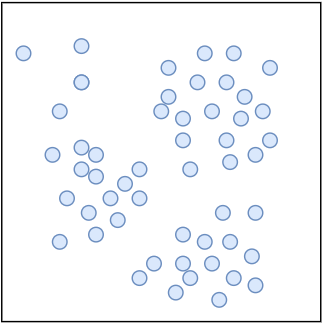
\includegraphics[width=1.0\linewidth]{images/glossary/unsupervised_learning_1_1.png}
				%\caption{}
			\end{figure}
			
			\column{0.05\linewidth}
			\begin{Huge}
				$$\pmb{\Rightarrow}$$
			\end{Huge}
			
			\pause

			\column{0.425\linewidth}
			\begin{figure}[!htbp]
				\centering
				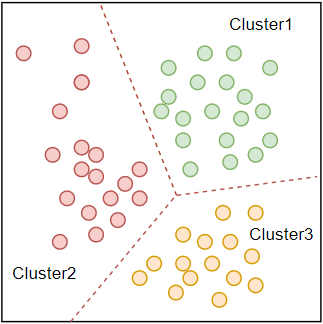
\includegraphics[width=1.0\linewidth]{images/glossary/unsupervised_learning_1_2.png}
				%\caption{}
			\end{figure}	
		\end{columns}

	\end{block}

\end{frame}


\begin{frame}

	\frametitle{Apprendimento non supervisionato}

	\begin{block}{Un esempio di apprendimento non supervisionato: il clustering}
	
		\begin{columns}
			\column{0.425\linewidth}
			\begin{figure}[!htbp]
				\centering
				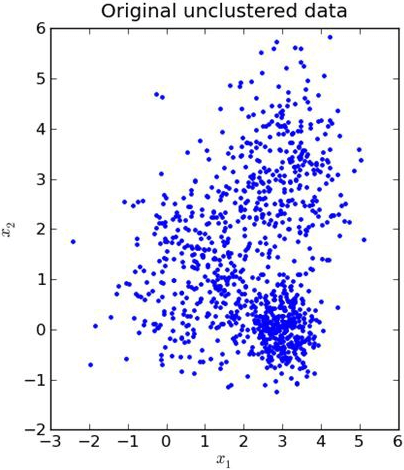
\includegraphics[width=1.0\linewidth]{images/glossary/unsupervised_learning_2_1.png}
				%\caption{Stripe Radar for Fraud Detection}
			\end{figure}
			
			\column{0.05\linewidth}
			\begin{Huge}
				$$\pmb{\Rightarrow}$$
			\end{Huge}
			
			\pause
			
			\column{0.425\linewidth}
			\begin{figure}[!htbp]
				\centering
				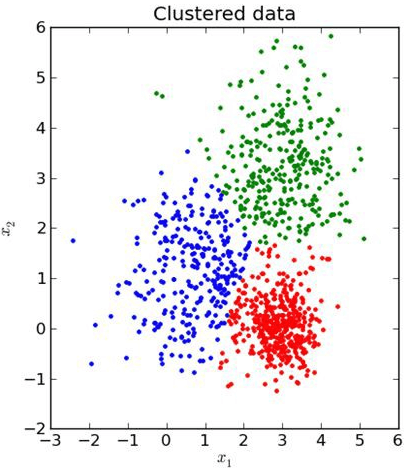
\includegraphics[width=1.0\linewidth]{images/glossary/unsupervised_learning_2_2.png}
				%\caption{Stripe Radar for Fraud Detection}
			\end{figure}	
		\end{columns}

	\end{block}

\end{frame}


\begin{frame}

	\frametitle{Apprendimento non supervisionato}

	\begin{block}{Un esempio di apprendimento non supervisionato con il \textbf{Mean Shift}}
		\begin{figure}[!htbp]
			\centering
			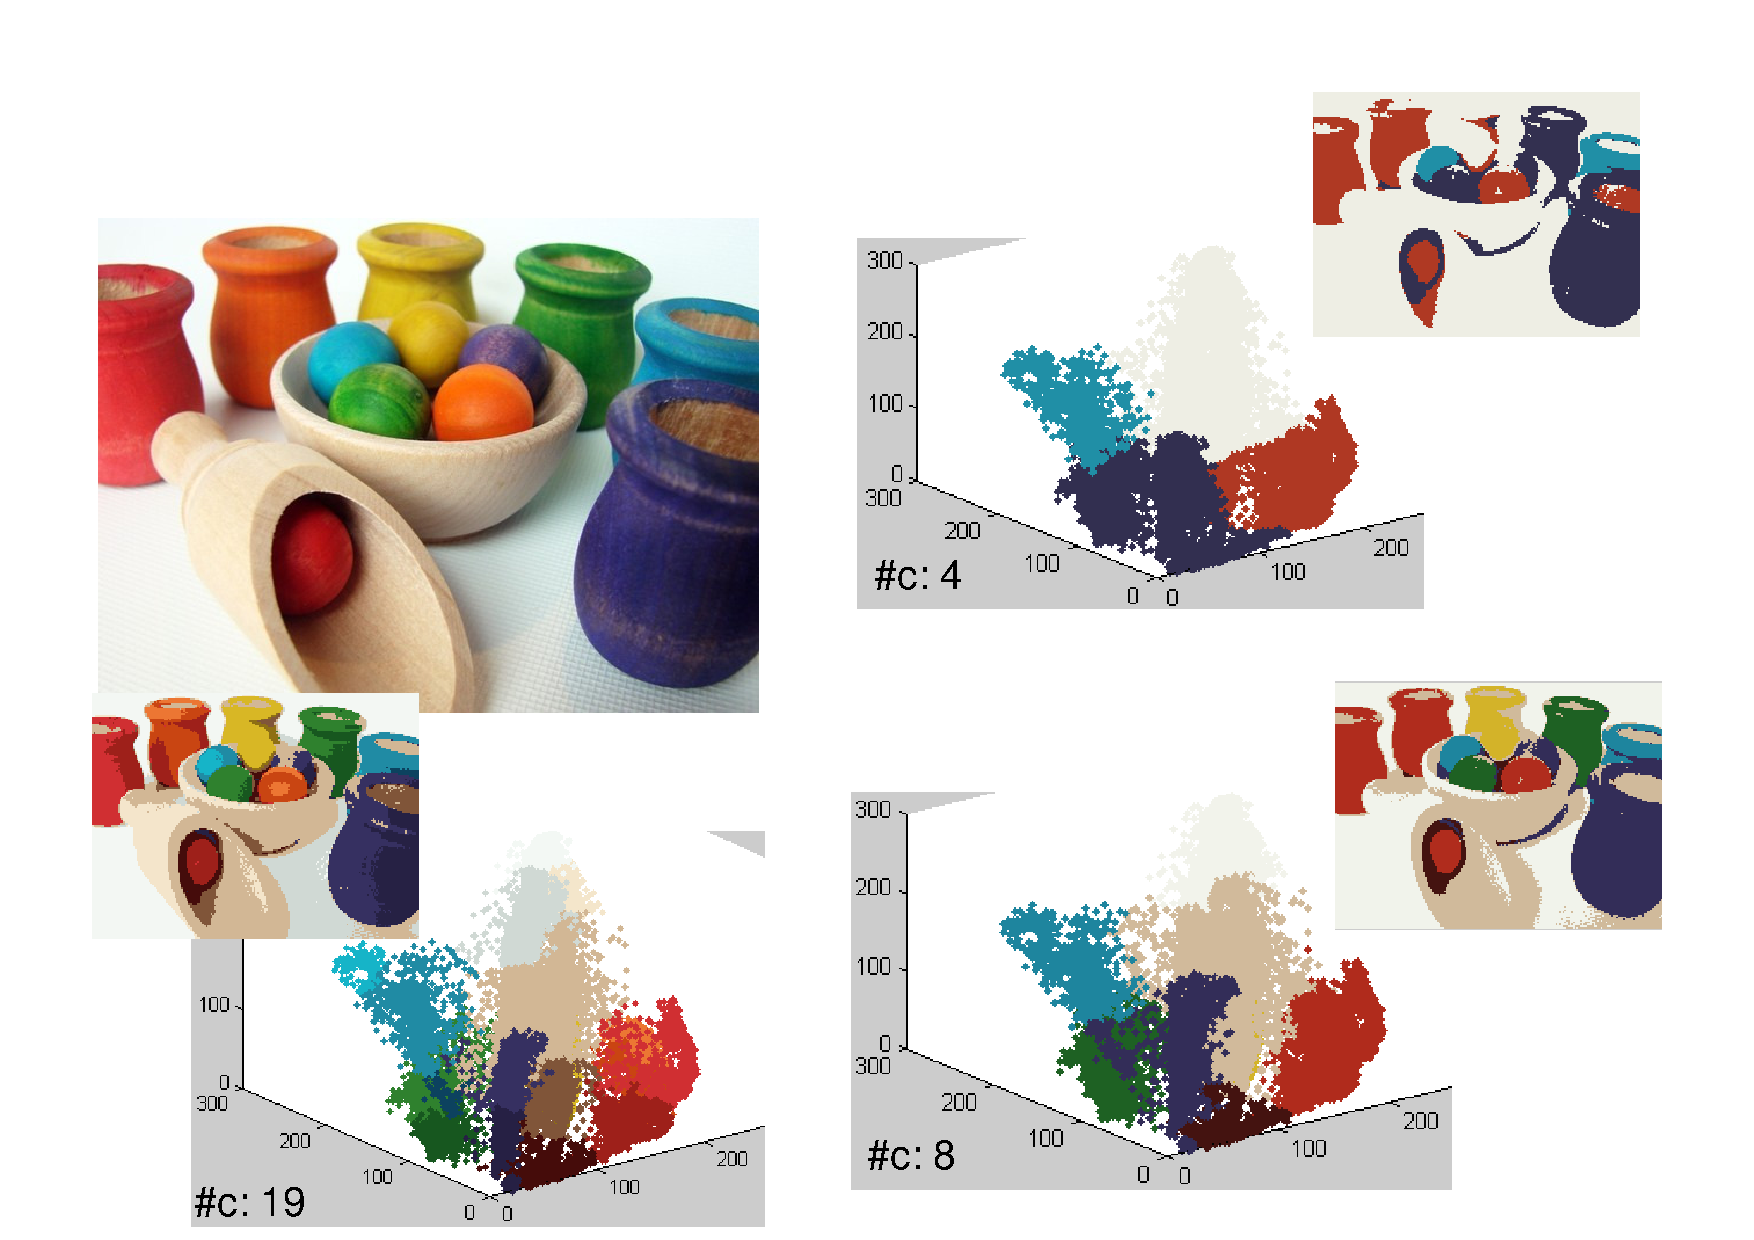
\includegraphics[width=8.5cm]{images/unsupervised/non_parametric/meanshift_pots.pdf}
			%\caption{Stripe Radar for Fraud Detection}
		\end{figure}

	\end{block}

\end{frame}



\subsubsection{Apprendimento supervisionato}
\begin{frame}

	\frametitle{Apprendimento supervisionato}

	\begin{block}{Qualche definizione}
		\begin{itemize}
			\item un algoritmo che impara da dati di esempio associati a risposte già pronte.\\
				Lo scopo di questo apprendimento è fare in modo che, quando all'algoritmo vengono sottoposti nuovi esempi, l'algoritmo stesso sia in grado di prevedere le risposte corrette
			\item prendere un dataset etichettato (labeled), indurre una regola generale per riuscire ad etichettare un nuovo dataset sprovvisto di etichette (unlabeled)
			\item vengono presentati degli input di esempio con associati  degli output desiderati, forniti da un ``insegnante'', e l'obiettivo è quello di apprendere una regola generale che mappa gli input sugli output
			\item in breve \textbf{functional approximation}
		\end{itemize}
	\end{block}

\end{frame}


\begin{frame}

	\frametitle{Apprendimento supervisionato}

	%\begin{block}{}

		Se vi viene data la seguente tabella:
		\begin{table}[]
			\begin{tabular}{ccccccccccc}
				\multicolumn{1}{c|}{input} 		& 1 & 2 & 3 & 4 & 5 & 6 & 7 & & 10 &  \\ \hline
				\multicolumn{1}{l|}{output}     & \undermat{labeled}{1 & 4 & 9 & 16 & 25 & 36 & 49 &} \undermat{unlabeled}{& ? &}  \\
			\end{tabular}
		\end{table}
		\vspace{5mm}

		\pause
		Molto probabilmente inferirete che la/il regola/modello è la/il seguente:
		$$output \leftarrow input^2 $$
		% Ma per affermare questo si fa un salto di fede (leap of faith)
		\pause
		Tuttavia esistono una miriade di altre regole/modelli che risultano essere comunque coerenti con il mapping mostrato (labeled):
		\begin{itemize}
			\item $output \leftarrow input^2$ eccetto per 10
			\item $output \leftarrow input^2$ per input tra 1 e 7; $output \leftarrow input$ altrimenti
			\item etc
		\end{itemize}


	%\end{block}



\end{frame}

\begin{frame}

	\frametitle{Apprendimento supervisionato}

	\begin{block}{Il problema della generalizzazione}
		Per utilizzare l'apprendimento supervisionato è necessario fare una assunzione fondamentale, ovvero che, attraverso i dati, sia possibile fare delle \textbf{generalizzazioni}.\\
	\end{block}

	\pause

	\begin{block}{Bias e inductive bias}
		Tutto il \ml e più nello specifico l'apprendimento supervisionato è basato sull'\textbf{induzione}.\\
		\textbf{Induzione}: passare da esempi ad una regola più generale,\\
		\hspace{31mm} dallo specifico al generale.
		\newlinedouble
		L'\textbf{inductive bias} (noto anche come \textbf{learning bias}) di un algoritmo di apprendimento è l'insieme delle assunzioni che il \textbf{learner} utilizza per\\ predire \textit{output} a partire da dati di \textit{input} che non ha ancora incontrato.
	\end{block}



\end{frame}

%\subsection[Glossario]{Glossario}



\begin{frame}

	\frametitle{Apprendimento supervisionato}

	\begin{block}{Deduction}
		L'induzione si contrappone alla \textbf{deduzione}, che consiste nel portare, tramite un ragionamento,
		da una regola generale ad uno più specifico.
		\newlinedouble
		Ad esempio: $A \implies B$, se $A$ è vero allora posso affermare che $B$ è vero.

	\end{block}


\end{frame}



\begin{frame}

	\frametitle{Apprendimento supervisionato}

	\begin{block}{Regressione vs. classificazione}
		L'apprendimento supervisionato può essere ulteriormente\\
		suddiviso in \textbf{due tipologie}:

		\begin{itemize}
			\item \textbf{modelli di regressione} che prevedono valori continui.\\
				\vspace{2mm}
				Ad esempio, i modelli di regressione fanno previsioni che rispondono a domande come le seguenti:
				\begin{itemize}
					\item[--] qual è il valore di una casa in California?
					\item[--] qual è la probabilità che un utente faccia clic su questo annuncio?
				\end{itemize}
				\vspace{2mm}
			\item \textbf{modelli di classificazione} che prevedono valori discreti.\\
				\vspace{2mm}
				Ad esempio, i modelli di classificazione fanno previsioni che rispondono a domande come le seguenti:
				\begin{itemize}
					\item[--] un determinato messaggio di posta elettronica è spam o non è spam?
					\item[--] è l'immagine di un cane, un gatto o un criceto?
				\end{itemize}
		\end{itemize}
	\end{block}


\end{frame}


\begin{frame}

	\frametitle{Apprendimento supervisionato}

	\begin{block}{Regressione vs. classificazione ($T_{C^{\circ}} = (T_{F^{\circ}} - 32) \times \frac{5}{9}$)}
		\begin{figure}[!htbp]
			\centering
			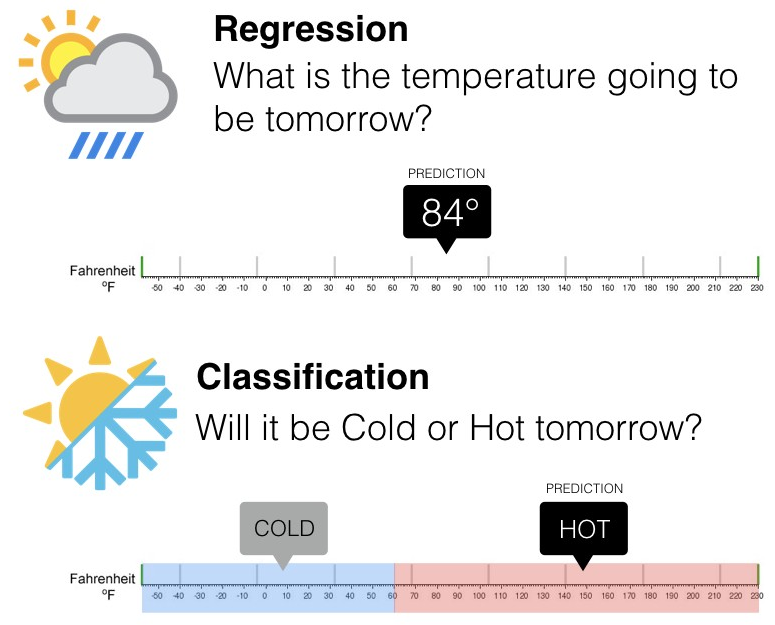
\includegraphics[width=7cm]{images/glossary/regression_vs_classification_2.png}
			%\caption{Stripe Radar for Fraud Detection}
		\end{figure}

	\end{block}

\end{frame}


\begin{frame}

	\frametitle{Apprendimento supervisionato}

	% Es twitter followers --> salary (for regression)
	\begin{block}{Regressione vs. classificazione}
		\begin{figure}[!htbp]
			\centering
			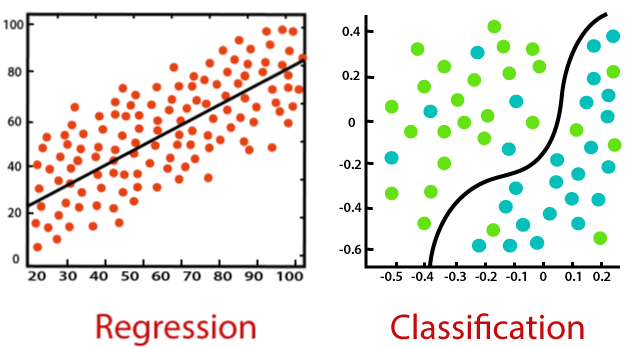
\includegraphics[width=10cm]{images/glossary/regression_vs_classification_1.png}
			%\caption{Stripe Radar for Fraud Detection}
		\end{figure}

	\end{block}

\end{frame}



\begin{frame}

	\frametitle{Glossario}
	\framesubtitle{introduciamo alcuni termini ricorrenti nel \ml}

	\begin{block}{Modello (il caso classico dell'apprendimento supervisionato)}
		\begin{figure}[!htbp]
			\centering
			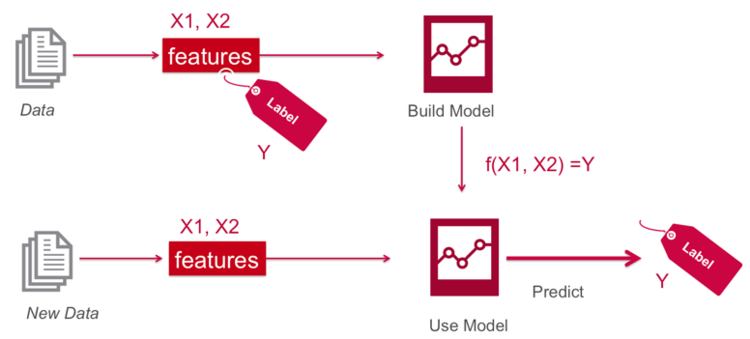
\includegraphics[width=11.9cm]{images/glossary/supervised_learning_1.png}
			%\caption{Stripe Radar for Fraud Detection}
			\label{fig:glossary_supervised_learning_1}
		\end{figure}

	\end{block}

\end{frame}


\begin{frame}

	\frametitle{Glossario}
	\framesubtitle{introduciamo alcuni termini ricorrenti nel \ml}

	\begin{block}{Modello (il caso classico dell'apprendimento supervisionato)}
		\begin{figure}[!htbp]
			\centering
			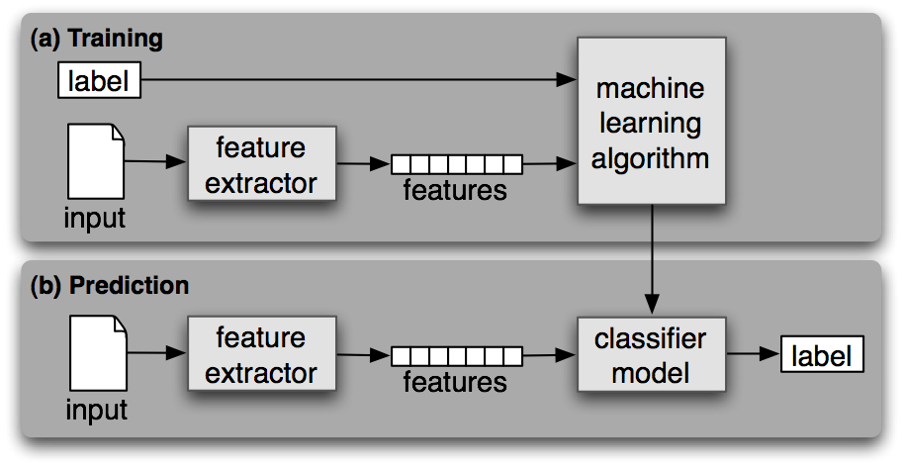
\includegraphics[width=11.2cm]{images/glossary/supervised_learning_2.png}
			\label{fig:glossary_supervised_learning_2}
			%\caption{Stripe Radar for Fraud Detection}
		\end{figure}

	\end{block}

\end{frame}


\begin{frame}

	\frametitle{Apprendimento: supervisionato vs non supervisionato}

	\begin{block}{}
		\begin{figure}[!htbp]
			\centering
			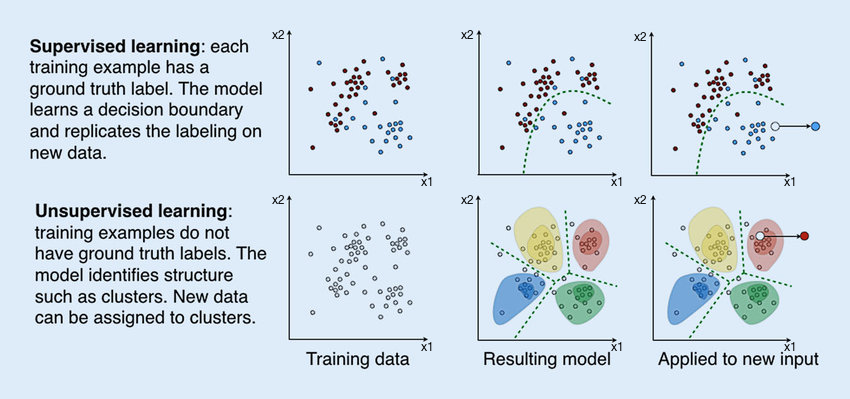
\includegraphics[width=12cm]{images/glossary/supervised_vs_unsupervised_1.png}
			%\caption{Stripe Radar for Fraud Detection}
		\end{figure}

	\end{block}

\end{frame}


\begin{frame}

	\frametitle{Apprendimento: supervisionato vs non supervisionato}

	\begin{block}{}
		\begin{figure}[!htbp]
			\centering
			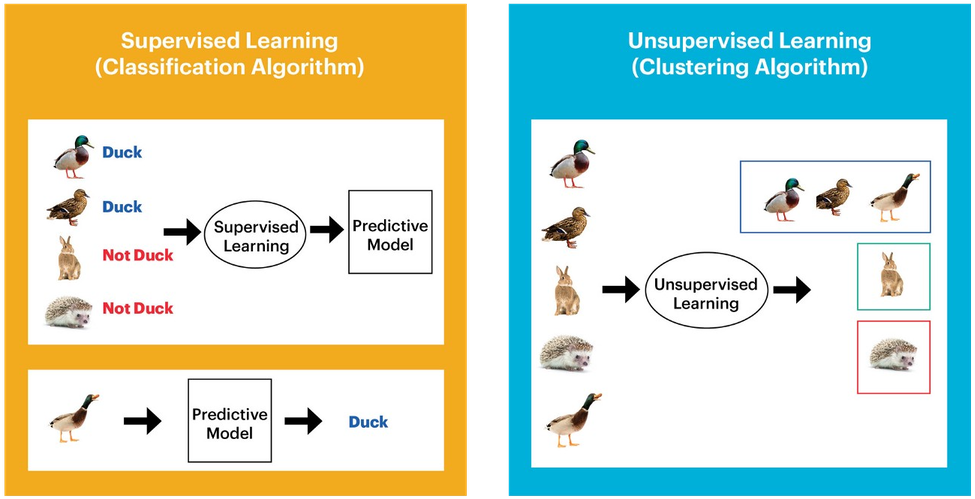
\includegraphics[width=12cm]{images/glossary/supervised_vs_unsupervised_2.png}
			%\caption{Stripe Radar for Fraud Detection}
		\end{figure}

	\end{block}

\end{frame}


\begin{frame}

	\frametitle{Apprendimento: supervisionato vs non supervisionato}

	\begin{block}{}
		\begin{figure}[!htbp]
			\centering
			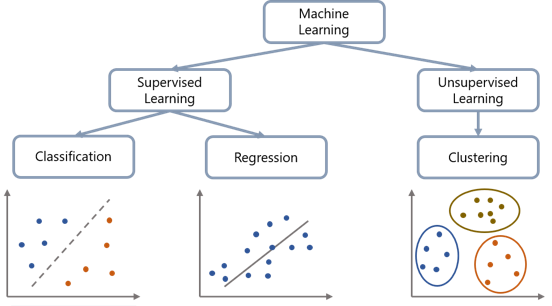
\includegraphics[width=12cm]{images/glossary/supervised_vs_unsupervised_3.png}
			%\caption{Stripe Radar for Fraud Detection}
		\end{figure}

	\end{block}

\end{frame}



\ifthenelse{\boolean{highschool}}{}{
	\subsubsection{Apprendimento per rinforzo}
	
	\begin{frame}
	
		\frametitle{Apprendimento per rinforzo}
	
		\begin{block}{Qualche definizione}
			\begin{itemize}
				\item si presentano all'algoritmo degli esempi privi di risposta associata, come nell'apprendimento non supervisionato; l'algoritmo può però proporre una soluzione agli esempi e \textbf{ricevere un feedback positivo o negativo} dal quale apprendere. L'apprendimento per rinforzo viene utilizzato con le applicazioni nelle quali l'algoritmo deve prendere delle decisioni da cui discendono delle conseguenze (pertanto il risultato dell'apprendimento è di tipo prescrittivo, cioè indica che cosa si dovrebbe fare, e non soltanto descrittivo, come invece accade nell'apprendimento non supervisionato)
				\item il modello interagisce con un ambiente dinamico nel quale cerca di raggiungere un obiettivo (per esempio guidare un veicolo), avendo un insegnante che gli dice solo se ha raggiunto l'obiettivo
				\item in breve \textbf{learning from delayed reward}
			\end{itemize}
	
		\end{block}
	
	
	\end{frame}
	
	
	\begin{frame}
	
		\frametitle{Apprendimento per rinforzo}
	
		\begin{block}{Osservazioni}
			\begin{itemize}
				\item nel mondo umano, è un po' come imparare con prove ed errori: gli ultimi aiutano a imparare, perché il fatto che vi sia implicato un costo (in termini economici, ma anche di perdita di tempo, dispiacere, dolore e così via) insegna che una certa linea di condotta ha potenzialmente meno probabilità di riuscita rispetto ad altre
				\item un interessante esempio di \textbf{apprendimento per rinforzo} si verifica quando i computer imparano autonomamente a giocare a un videogioco.\\
				In questo caso, un'applicazione presenta all'algoritmo degli esempi di situazioni specifiche di gioco. L'applicazione fa conoscere all'algoritmo il risultato delle azioni che potrebbe intraprendere e l'apprendimento si verifica allorché l'algoritmo cerca di evitare ciò che scopre essere pericoloso e cerca di continuare a sopravvivere nel gioco.
			\end{itemize}
		\end{block}
	
	\end{frame}
	
	
	\begin{frame}
	
		\frametitle{Apprendimento per rinforzo}
	
		\begin{block}{Osservazioni}
	
			\begin{columns}
	
				\column{0.6\linewidth}
				\begin{itemize}
					\item Su YouTube all'indirizzo \href{https://www.youtube.com/watch?v=V1eYniJ0Rnk}{\underline{Google DeepMind's Deep Q-learning playing Atari Breakout}} potete osservare in che modo \textbf{DeepMind} ha sviluppato un programma di apprendimento per rinforzo che gioca a un videogame Atari del passato. Osservando il video, si nota che, all'inizio, il programma è piuttosto imbranato e non particolarmente abile nel gioco, ma attraverso l’apprendimento migliora a mano a mano, fino a diventare un campione
				\end{itemize}
	
				\column{0.4\linewidth}
				\begin{figure}[!htbp]
					\centering
					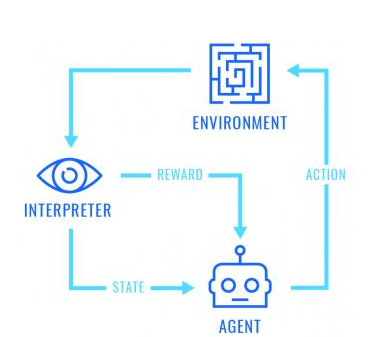
\includegraphics[width=5cm]{images/glossary/reinforcement_learning.png}
					%\caption{Stripe Radar for Fraud Detection}
				\end{figure}
	
			\end{columns}
	
		\end{block}
	
	\end{frame}


	\begin{frame}
	
		\frametitle{Le tipologie di apprendimento}
	
		\begin{block}{L'ottimizzazione}
				Tutte queste categorie di apprendimento automatico sono \textbf{interconnesse}.\\
				Infatti si potrebbe formulare ognuno di questi problemi sottoforma di un \textbf{problema di ottimizzazione}:
				\begin{figure}[!htbp]
					\centering
					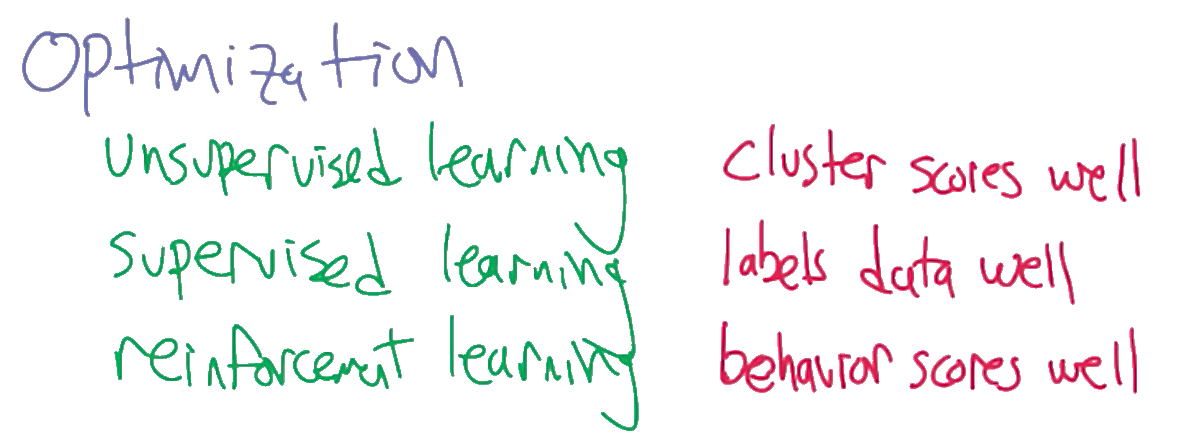
\includegraphics[width=11cm]{images/glossary/optimization.png}
					%\caption{Stripe Radar for Fraud Detection}
				\end{figure}
		\end{block}
	
	\end{frame}
}

\ifthenelse{\boolean{highschool}}{}{
\section[Data prep (preparazione e preprocessing)]{Data prep (preparazione e preprocessing)}
\sectionframe{images/covers/cover_data_preparation.png}{Data prep}

\subsection[Gettare le fondamenta dell'apprendimento]{Gettare le fondamenta dell'apprendimento}
\begin{frame}
	\frametitle{Data prep: gettare le fondamenta dell'apprendimento}
	
%	\begin{block}{}
		Prima di passare a visionare i \textbf{modelli di apprendimento automatico più diffusi} con i relativi algoritmi, come si può anche osservare in figura, bisogna soffermarci sulle operazioni necessarie a monte del processo di apprendimento: \textbf{la preparazione e il preprocessing dei dati}.
		\newlinedouble
		Quando si costruisce una nuova casa, ci sono cose più importanti da fare prima di pensare alla bellezza dell'architettura o ai particolari estetici.\\
		Prima di tutto ciò vanno \textbf{realizzare delle solide fondamenta} su cui poi innalzare i muri.\\
		Se non si preparano bene le fondamenta – ossia i dati – l'algoritmo non reggerà a lungo quando verrà testato in situazioni in cui si presentano dati reali.
		\begin{figure}[!htbp]
			\centering
			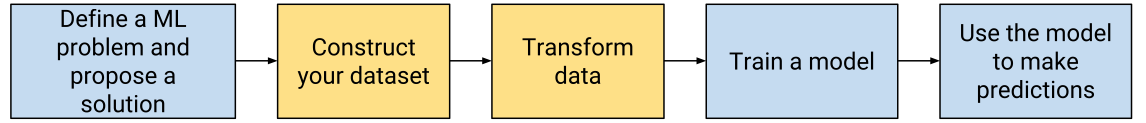
\includegraphics[width=0.9\linewidth]{images/data_prep/build_the_foundation/5phases.png}
					%\caption{Stripe Radar for Fraud Detection}
		\end{figure}

		
%	\end{block}

\end{frame}


%% Per raccogliere e ripulire --> aggiungere il feature enginering
% e il quality of good features


\begin{frame}
	
	\frametitle{Data prep}
	
%	\begin{block}{}
	La \textbf{preparazione e il preprocessing dei dati} consiste in diversi passaggi:
	\begin{enumerate}
		\item ottenere il ground truth, ossia i dati che qualcuno ha correttamente misurato o etichettato
		\item acquisire dati sufficienti da dare in pasto all'algoritmo di apprendimento. Non è possibile sapere a priori quanti sono i dati di cui avrete bisogno, perché tutto dipende dall'algoritmo utilizzato: solo dopo il test riuscirete a capire se le vostre stime soffrono di un eccesso di bias o di varianza dell'algoritmo che avete deciso di adottare
		\item sistemare i dati che avete raccolto in una matrice
		\item gestire i dati problematici, come i casi mancanti (un problema frequente), le distribuzioni distorte, le ridondanze e gli esempi anomali
		\item creare nuove feature (quando occorrono) che risultino particolarmente adatte a fare in modo che l'algoritmo impari come mappare la risposta
	\end{enumerate}
			
%	\end{block}

\end{frame}


\begin{frame}
	
	\frametitle{Data prep}
	
%	\begin{block}{}
		%Tra le operazioni più importanti che spesso è opportuno adottate nella fase di \textbf{preparazione dei dati} ci sono le seguenti:
		Dividiamo quindi i vari task coinvolti nella \textbf{preparazione dei dati} nei seguenti macrogruppi:\\
		\begin{itemize}
			\item {\color{GradientDescentDiagramBlue}raccogliere e ripulire i dati}
			\item {\color{GradientDescentDiagramGreen}sistemare i dati mancanti}
			\item {\color{GradientDescentDiagramOrange}trasformare le distribuzioni}
			\item {\color{GradientDescentDiagramRed}creare proprie features}
			\item etc...
		\end{itemize}		
%	\end{block}

\end{frame} 
\subsection[Raccogliere e ripulire i dati]{Raccogliere e ripulire i dati}

\begin{frame}

	\frametitle{{\color{GradientDescentDiagramBlue}Raccogliere e ripulire i dati}}

%	\begin{block}{}
		Quando si tratta di dati, \textbf{non esiste una ricetta magica}, come afferma:
		\begin{itemize}
			\item il \textbf{No Free Lunch Theorem} (Wolpert, 1996):\\
				\emph{Non esiste un modello o algoritmo di stima universalmente ottimale}
			\item Ogni modello o algoritmo di stima è basato su uno specifico insieme di ipotesi, che può funzionare bene o meno a seconda dell'applicazione in questione. Ecco perchè è importante acquisire familiarità con molti \textbf{tipi diversi di modelli e metodi di stima}
%			\item Esempio:
%
%			\begin{itemize}
%				\item Supponiamo di disporre di $p=100$ predittori binari
%				\item Il numero delle combinazioni possibili degli input è $2^{100} = 1267650600228229401496703205376$
%				\item Non avremo \emph{mai} un campione che contiene un'osservazione della $Y$ per ognuna di queste possibili combinazioni
%				\item Com'è possibile allora che un modello fornisca una previsione $\hat y$ per ognuna di esse? \emph{Grazie alla struttura che implicitamente il modello impone sui dati}
%				\item A seconda dell'applicazione, la struttura può funzionare o meno\ldots
%			\end{itemize}
		\end{itemize}

		Inoltre anche le funzioni di apprendimento più sofisticate e avanzate non ce la fanno e finiscono per avere pessime prestazioni se non le supportate con quanto segue:
		\begin{itemize}
			\item \textbf{quantità di dati sufficientemente grandi} da essere adeguate all'algoritmo che state utilizzando
			\item \textbf{dati puliti e ben preparati} da utilizzare con il machine learning (secondo il principio GIGO = Garbage In, Garbage Out)
		\end{itemize}
%	\end{block}

%Al di là della quantità dei dati, è comprensibile la necessità della loro pulizia. È un po' come la qualità degli insegnamenti che ricevete a scuola: se gli insegnanti vi insegnano solo cose senza senso, vi presentano esempi sbagliati, passano il tempo a scherzare e, in generale, non prendono seriamente l'insegnamento, i vostri esami non potranno andare granché bene, per quanto possiate essere intelligenti. Lo stesso vale sia per gli algoritmi semplici sia per quelli complessi: se li rifocillate di dati spazzatura, le previsioni prodotte non potranno che essere prive di senso.
%Secondo il principio del garbage in, garbage out (o GIGO, letteralmente “spazzatura dentro, spazzatura fuori”, ossia se elabori spazzatura non puoi che ottenere spazzatura, banale ma assolutamente vero), se i dati sono di cattiva qualità il processo di machine learning ne può risultare seriamente compromesso. Con dati di cattiva qualità si intendono dataset presentanti dati mancanti, valori anomali, intere feature composte di valori distorti, ridondanza di informazioni. In questo capitolo tutti questi problemi vengono affrontati, unitamente alle relative possibili soluzioni.

\end{frame}


\subsubsection[Mappare dati grezzi in features]{Mappare dati grezzi in features}
\begin{frame}

	\frametitle{{\color{GradientDescentDiagramBlue}Raccogliere e ripulire i dati}: mappare dati grezzi in features}

%	\begin{block}{Mappare i dati grezzi in features}
%		I dati di cattiva qualità potrebbero non essere di per sé sbagliati:
%		\begin{itemize}
%			\item dati che non ottemperano agli \textbf{standard}
%			\item \textbf{date scritte in formati non validi}
%			\item \textbf{testo non strutturato} da convertire in variabile categorica
%		\end{itemize}
		All'interno di questa fase di raccolta dobbiamo includere anche il \textbf{feature engineering} ovvero il processo con il quale si trasformano i dati grezzi in un vettore di fetures.
		\newlinedouble
		Molti modelli di machine learning devono rappresentare le features come vettori di numeri reali poiché i valori delle features devono essere moltiplicati per i pesi del modello.

		\begin{figure}[!htbp]
			\centering
			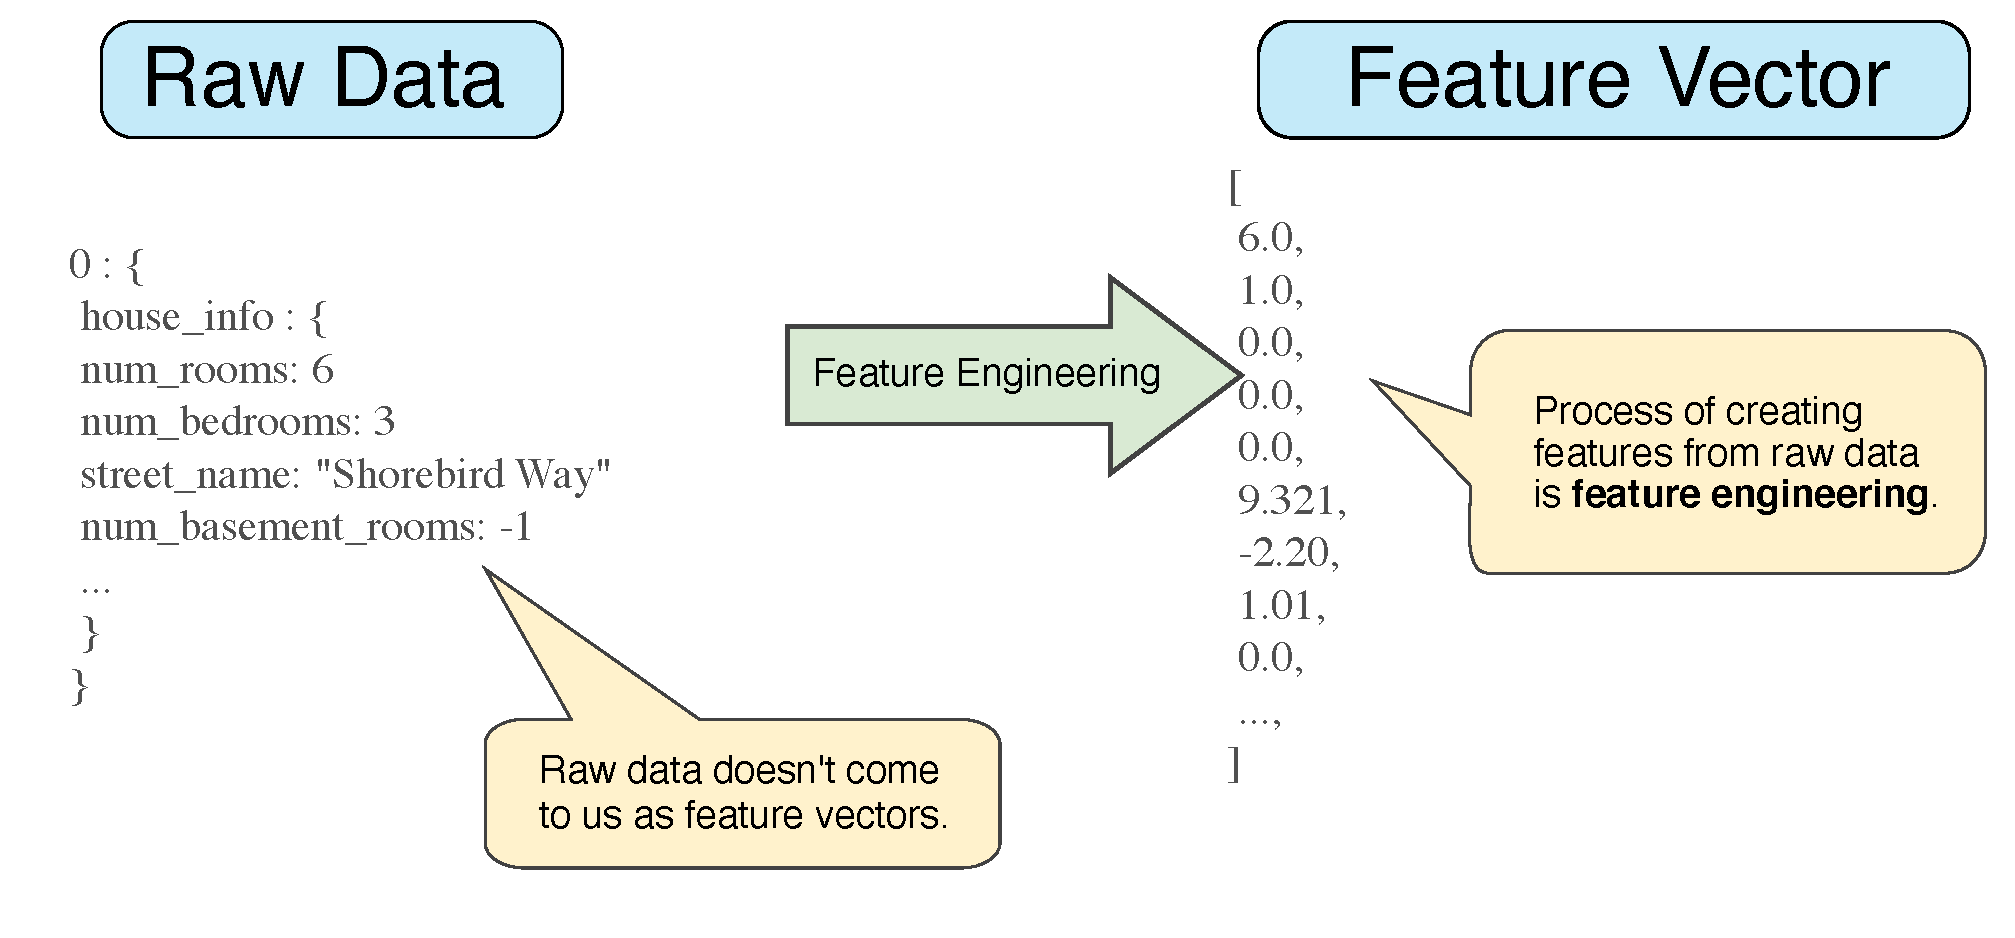
\includegraphics[width=0.75\linewidth]{images/data_prep/feature_engineering_and_data_cleaning/RawDataToFeatureVector.pdf}
					%\caption{Stripe Radar for Fraud Detection}
		\end{figure}
%	\end{block}

\end{frame}


\subsubsection[Mappare valori numerici]{Mappare valori numerici}
\begin{frame}

	\frametitle{{\color{GradientDescentDiagramBlue}Raccogliere e ripulire i dati}: mappare valori numerici}

%	\begin{block}{}
		I dati interi e in virgola mobile non necessitano di una codifica speciale perché possono essere moltiplicati per un peso numerico.\\
		Come suggerito nella figura mostrata, la conversione del valore intero grezzo 6 nel valore della feature 6.0 è procedimento scontato:
		\begin{figure}[!htbp]
			\centering
			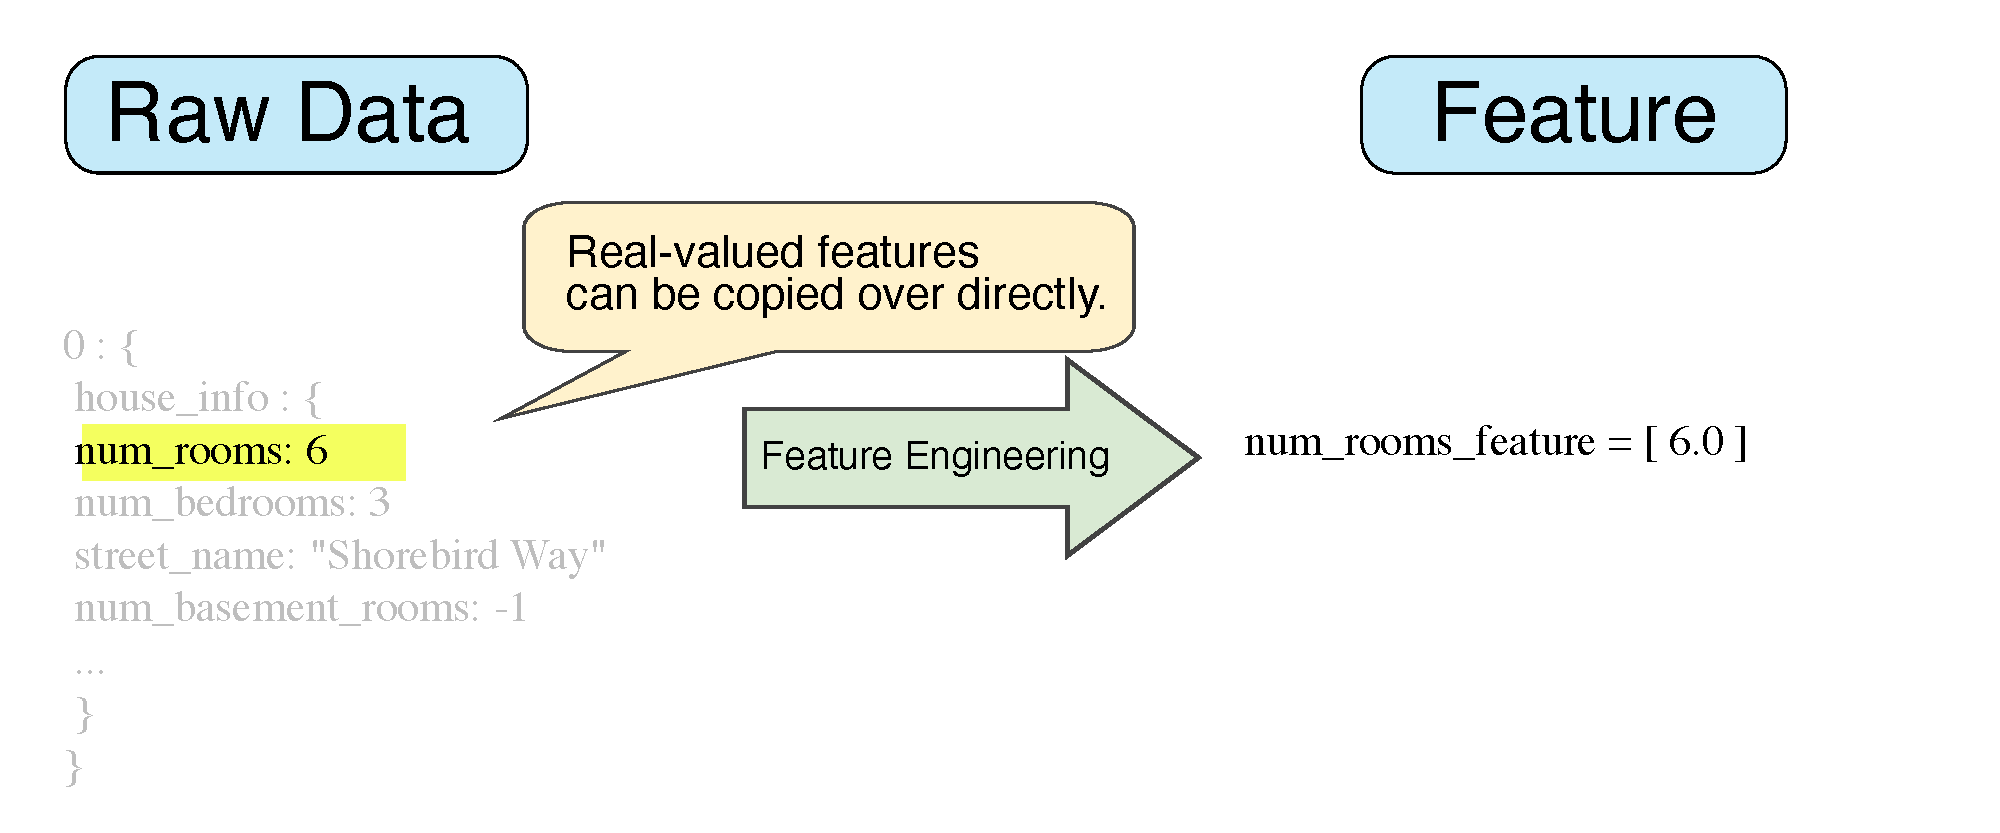
\includegraphics[width=1.0\linewidth]{images/data_prep/feature_engineering_and_data_cleaning/FloatingPointFeatures.pdf}
					%\caption{Stripe Radar for Fraud Detection}
		\end{figure}

%	\end{block}

\end{frame}


\subsubsection[Mappare valori numerici]{Mappare valori categorici}
\begin{frame}

	\frametitle{{\color{GradientDescentDiagramBlue}Raccogliere e ripulire i dati}: mappare valori categorici}

%	\begin{block}{}
		Le features categoriche hanno un insieme discreto di possibili valori.\\
		Ad esempio, potrebbe esserci una feature chiamata \textit{street\_name} con valori che includono:
		\begin{scriptsize}
			\begin{empheq}[box=\fcolorbox{blue!40!black!60}{yellow!10}]{align*}
				\text{\{'Charleston Road', 'North Shoreline Boulevard', 'Shorebird Way', 'Rengstorff Avenue'\}}
			\end{empheq}
		\end{scriptsize}

		Poiché i modelli non possono moltiplicare le stringhe per i pesi appresi, utilizziamo la feature engineering per \textbf{convertire le stringhe in dei valori numerici}.

%	\end{block}

\end{frame}


\begin{frame}

	\frametitle{{\color{GradientDescentDiagramBlue}Raccogliere e ripulire i dati}: mappare valori categorici}

%	\begin{block}{}
		Alcune soluzioni:
		\begin{itemize}
			\item \textbf{mappare il vocabolario in differenti valori interi}. Poiché non tutte le strade del mondo appariranno nel nostro dataset, possiamo raggruppare tutte le altre strade in una categoria chiamata \textit{altro} generico, nota come bucket OOV (out-of-vocabulary)
				\begin{itemize}
					\item[--] questi valori numerici così imposti potrebbero non avere una relazione lineare con la label da predire. Modelli poco flessibili non saranno in grado di utilizzare questa feature in modo adeguato
					\item[--] non è possibile codificare una relazione uno a molti (se ad esempio una casa è ad un incrocio)
				\end{itemize}
			\item \textbf{one-hot encoding}: creare un vettore binario per ogni feature categorica nel nostro modello che rappresenta i valori come segue:
				\begin{itemize}
					\item[--] il vettore varrà 1 in corrispondenza della posizione del vettore che matcha lo specifico valore categorico
					\item[--] 0 su tutti gli altri
				\end{itemize}
			\item \textbf{multi-hot encoding}: simile al \textit{one-hot encoding} ma prevede la possibilità di più di un solo 1 nel vettore
		\end{itemize}



%	\end{block}

\end{frame}


\begin{frame}

	\frametitle{{\color{GradientDescentDiagramBlue}Raccogliere e ripulire i dati}}

	\begin{block}{}

		\begin{figure}[!htbp]
			\centering
			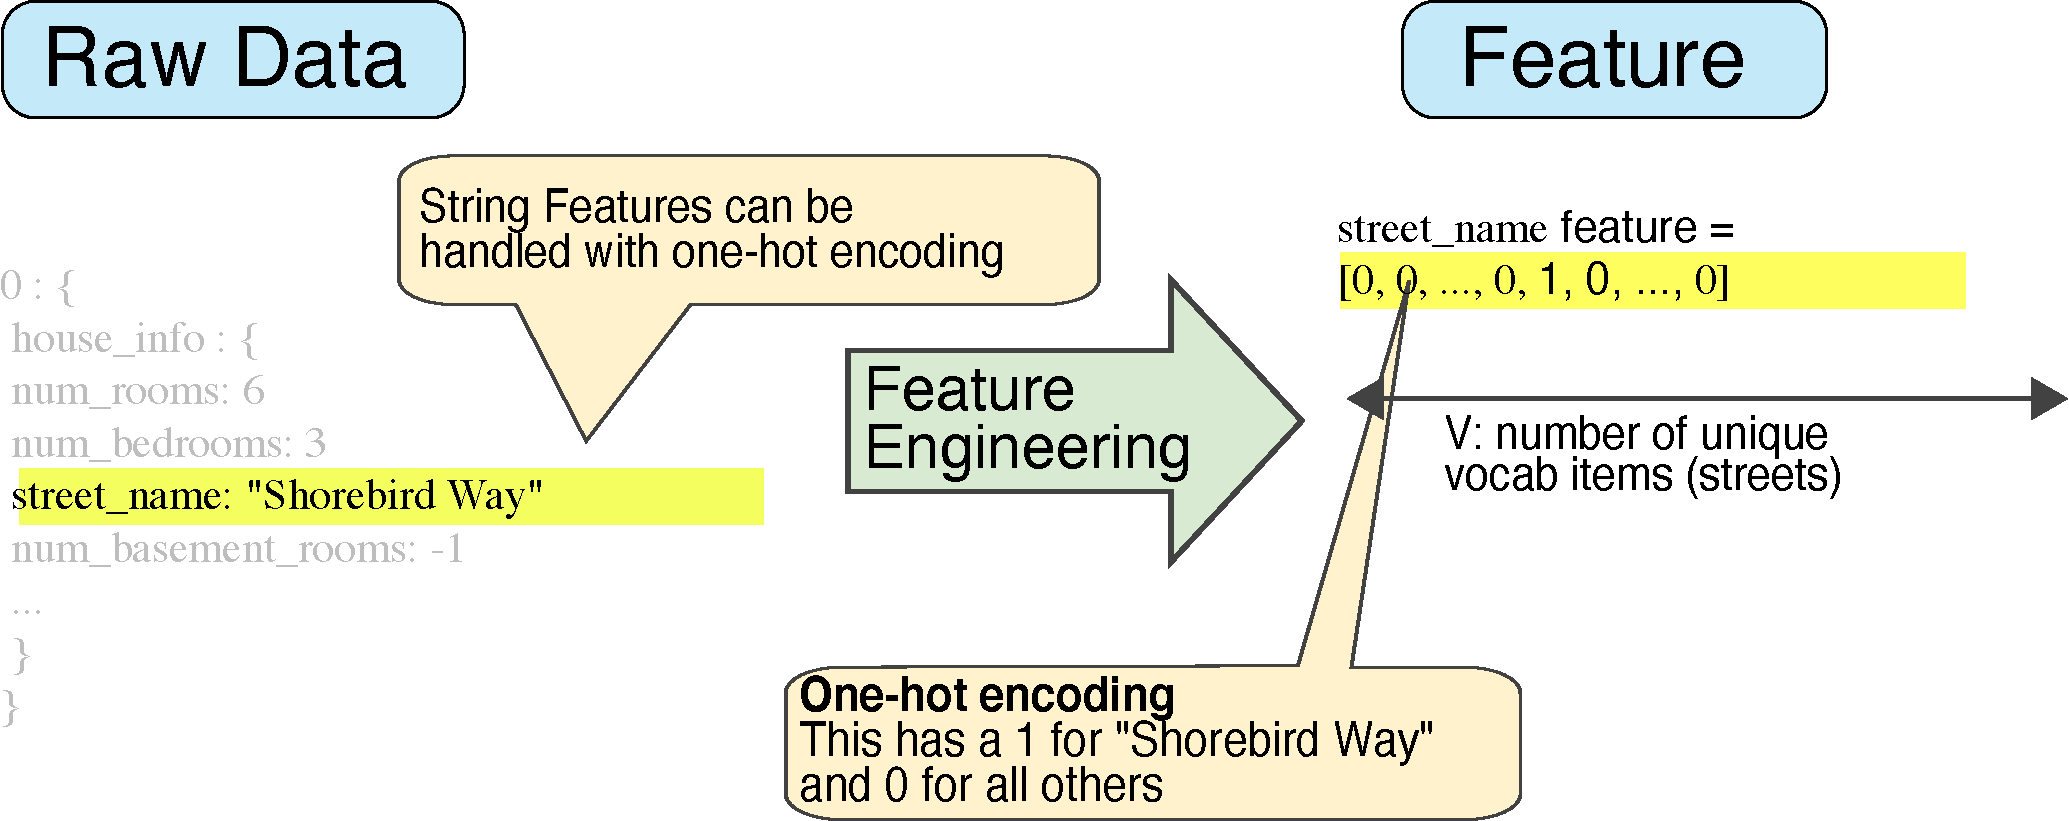
\includegraphics[width=1.0\linewidth]{images/data_prep/feature_engineering_and_data_cleaning/OneHotEncoding.pdf}
					%\caption{Stripe Radar for Fraud Detection}
		\end{figure}

	\end{block}

\end{frame}


\begin{frame}

	\frametitle{{\color{GradientDescentDiagramBlue}Raccogliere e ripulire i dati}}

	\begin{block}{Alcune linee guida per costruzione e l'uso di buone features}
		\begin{itemize}
			\item evitare valori di elementi discreti usati raramente
			\item ogni feature dovrebbe avere un significato chiaro e il più ovvio possibile
			\item non mischiare \textbf{magic numbers} con dati reali
			\item la definizione di una feature non dovrebbe cambiare nel tempo
		\end{itemize}
	\end{block}

\end{frame}


\subsubsection[Mappare valori numerici]{Ripulire i dati: lo scrubbing}
\begin{frame}

	\frametitle{{\color{GradientDescentDiagramBlue}Raccogliere e ripulire i dati}}

	\begin{block}{Ripulire i dati: lo scrubbing}
		Fino ad ora, abbiamo ipotizzato che tutti i dati utilizzati per l'addestramento e il test fossero affidabili.\\
		\vspace{1mm}
		Nella vita reale, molti esempi dataset non sono affidabili a causa di uno o più dei seguenti motivi:

		\begin{itemize}
			\item \textbf{valori omessi}. Ad esempio, una persona ha dimenticato di inserire un valore per l'età di una casa
			\item \textbf{esempi duplicati}. Ad esempio, un server ha erroneamente caricato due volte gli stessi log
			\item \textbf{etichette sbagliate}. Ad esempio, una persona ha erroneamente etichettato l'immagine di una quercia come un acero
			\item \textbf{valori di feature errati}. Ad esempio, qualcuno ha digitato una cifra in più
		\end{itemize}

	\end{block}

\end{frame}

\subsection[Sistemare i dati mancanti]{Sistemare i dati mancanti}

\begin{frame}
	\frametitle{{\color{GradientDescentDiagramGreen}Sistemare i dati mancanti}}

	%\begin{block}{}
		La presenza di un \textbf{esempio incompleto} rende impossibile connettere tutti i segnali all'interno delle feature e tra feature diverse. Inoltre, se ci sono valori mancanti per molti algoritmi risulta impossibile riuscire ad apprendere durante la fase di addestramento.
		\newlinedouble
		Di conseguenza, è necessario \textbf{sostituire tutti i valori mancanti} della matrice di dati con valori adatti a fare in modo che l’algoritmo di apprendimento funzioni correttamente.
		\newlinedouble
		I \textbf{motivi} che causano la mancanza di valori possono essere i \textbf{più disparati}.\\
		Per gestire in modo efficace i dati mancanti, le strategie possibili sono diverse e possono cambiare se dovete gestire valori mancanti all’interno di feature quantitative o qualitative.
	%\end{block}
	
\end{frame}


\begin{frame}
	\frametitle{{\color{GradientDescentDiagramGreen}Sistemare i dati mancanti}: strategie di sostituzione}

	%\begin{block}{}
		Di seguito sono riportate alcune delle strategie più comuni per la gestione dei dati mancanti:
		\begin{itemize}
			\item sostituire i valori mancanti con una \textbf{costante calcolata come il valore medio o mediano} (per le categoriche andrà fornito un valore categorico)
			\item sostituire i valori mancanti con un \textbf{valore all’esterno a quello del normale range} di valori della feature (ideale da adoperare con gli algoritmi basati sugli alberi di decisione e variabili qualitative)
			\item sostituire i valori mancanti \textbf{con 0}, che funziona bene con i modelli di regressione e le variabili standardizzate (anche qualitative binarie)
			\item \textbf{interpolare i valori} mancanti quando fanno parte di una serie di valori legati al tempo
			\item \textbf{predire il valore} utilizzando le informazioni presenti in altre feature che fungono da predittori (ma non utilizzare mai la variabile di risposta)
		\end{itemize}
	%\end{block}
	
\end{frame}
\subsection[Trasformare le distribuzioni]{Trasformare le distribuzioni}

\begin{frame}
	
	\frametitle{{\color{GradientDescentDiagramOrange}Trasformare le distribuzioni}}
	
	
	%In clustering, you calculate the similarity between two examples by combining all the feature data for those examples into a numeric value. Combining feature data requires that the data have the same scale. This section looks at normalizing, transforming, and creating quantiles, and discusses why quantiles are the best default choice for transforming any data distribution. Having a default choice lets you transform your data without inspecting the data's distribution.
	
	%\begin{block}{}
		Partiamo da un esempio: nel clustering, si calcola la similarità/dissimilarità tra due esempi prendendo in considerazione tutte le features numeriche.
		Utilizzando le features numeriche per utilizzare una metrica tra gli esempi è necessario che i dati siano nella stessa scala.
		\newlinedouble
		Il clustering è solo un esempio, molti altri algoritmi di apprendimento automatico richiedono che queste condizioni di scala nei dati utilizzati siano verificate al fine di funzionare efficientemente.
		\newlinedouble
		Esaminiamo quindi le operazioni più comuni applicate prima procedere con l'esecuzione degli algoritmi di apprendimento automatico:
		\begin{itemize}
			\item {\color{GradientDescentDiagramBlue}normalizzazione}
			\item {\color{GradientDescentDiagramRed}log-transform}
			\item {\color{GradientDescentDiagramGreen}quantili}
		\end{itemize}
	%\end{block}
	
\end{frame}





\subsubsection[Normalizzazione]{Normalizzazione}
\begin{frame}
	
	\frametitle{{\color{GradientDescentDiagramOrange}Trasformare le distribuzioni}: {\color{GradientDescentDiagramBlue}normalizzazione}}
	
	%\begin{block}{}
		È possibile trasformare i dati per più features nella stessa scala normalizzando i dati.
		In particolare, la normalizzazione è adatta per elaborare la distribuzione dei dati più comune, la \textbf{distribuzione gaussiana}.
		Rispetto ai quantili, la normalizzazione richiede un numero significativamente inferiore di dati per il calcolo.
		\newlinedouble
		Possiamo normalizzare i dati calcolando il relativo \textbf{z-score} come segue:
		\begin{empheq}[box=\fcolorbox{blue!40!black!60}{yellow!10}]{align*}
		x' = \frac{(x-\mu)}{\sigma} \quad:\quad\mu = \text{mean},\text{ }\sigma = \text{standard deviation}
		\end{empheq}
		
	%\end{block}
	
\end{frame}


\begin{frame}
	
	\frametitle{{\color{GradientDescentDiagramOrange}Trasformare le distribuzioni}: {\color{GradientDescentDiagramBlue}normalizzazione}}
	
	%\begin{block}{}
		Diamo un'occhiata alla somiglianza tra esempi normalizzati e non.	 Dalla figura mostrata sembrerebbe che il rosso è più simile al blu che al giallo.\\
		Tuttavia, le features sugli assi $x$ e $y$ \textbf{non hanno la stessa scala}.
		%Pertanto, la somiglianza osservata potrebbe essere legata al fatto che i dati non sono scalati.
		\newlinedouble
		Dopo la normalizzazione, tutte le features hanno la stessa scala; adesso in effetti il rosso è più simile al giallo. Pertanto, dopo aver normalizzato i dati, è possibile calcolare la somiglianza in modo più accurato.
		
		\begin{figure}[!htbp]
			\centering
			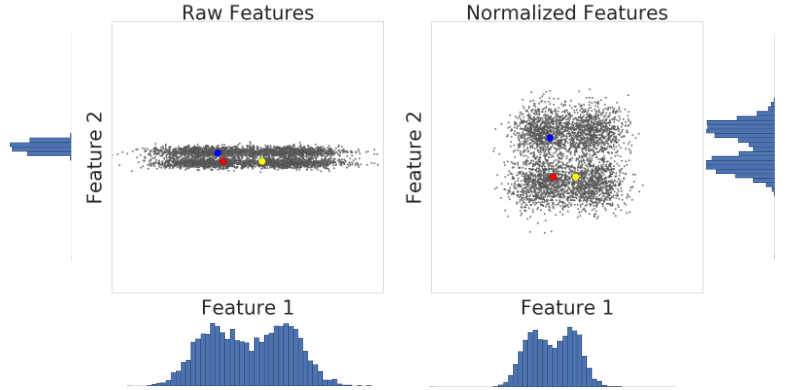
\includegraphics[width=8.0cm]{images/data_prep/scaling_distributions/NormalizeData.png}
					%\caption{Stripe Radar for Fraud Detection}
		\end{figure}
		
	%\end{block}
	
\end{frame}


\begin{frame}
	
	\frametitle{{\color{GradientDescentDiagramOrange}Trasformare le distribuzioni}: {\color{GradientDescentDiagramBlue}normalizzazione}}
	
	\begin{block}{Quando è opportuno normalizzare?}
		In sintesi, è opportuno applicare la normalizzazione quando una delle seguenti condizioni risulta verificata:
		\begin{itemize}
			\item i tuoi dati hanno una distribuzione gaussiana
			\item il tuo dataset non dispone di dati sufficienti per creare quantili
		\end{itemize}
	\end{block}
	
	\begin{block}{La normalizzazione min-max}
		Abbiamo visto la cosiddetta \textbf{normalizzazione z-score}, tuttavia a volte si preferisce utilizzare un'altro tipo di normalizzazione, più semplice, detta \textbf{normalizzazione min-max}:
		\begin{empheq}[box=\fcolorbox{blue!40!black!60}{yellow!10}]{align*}
		x' = \frac{x-min}{max-min} \quad:\quad min = \underset{\forall i \in D}{min}\text{ }x_i,\text{ }max = \underset{\forall i \in D}{max}\text{ }x_i
		\end{empheq}
	\end{block}
	
\end{frame}

\subsubsection[Log-Transform]{Log-Transform}
\begin{frame}
	
	\frametitle{{\color{GradientDescentDiagramOrange}Trasformare le distribuzioni}: {\color{GradientDescentDiagramRed}log-transform}}
		
	%\begin{block}{Quando è necessario normalizzare?}
		A volte, un dataset è conforme alla distribuzione \textbf{power law} ($f(x) = ax^k + o(x^k), \ x \to 0$) che raggruppa i dati all'estremità inferiore.\\
		%Nella figura, il rosso è più vicino al giallo che al blu.
		\begin{figure}[!htbp]
			\centering
			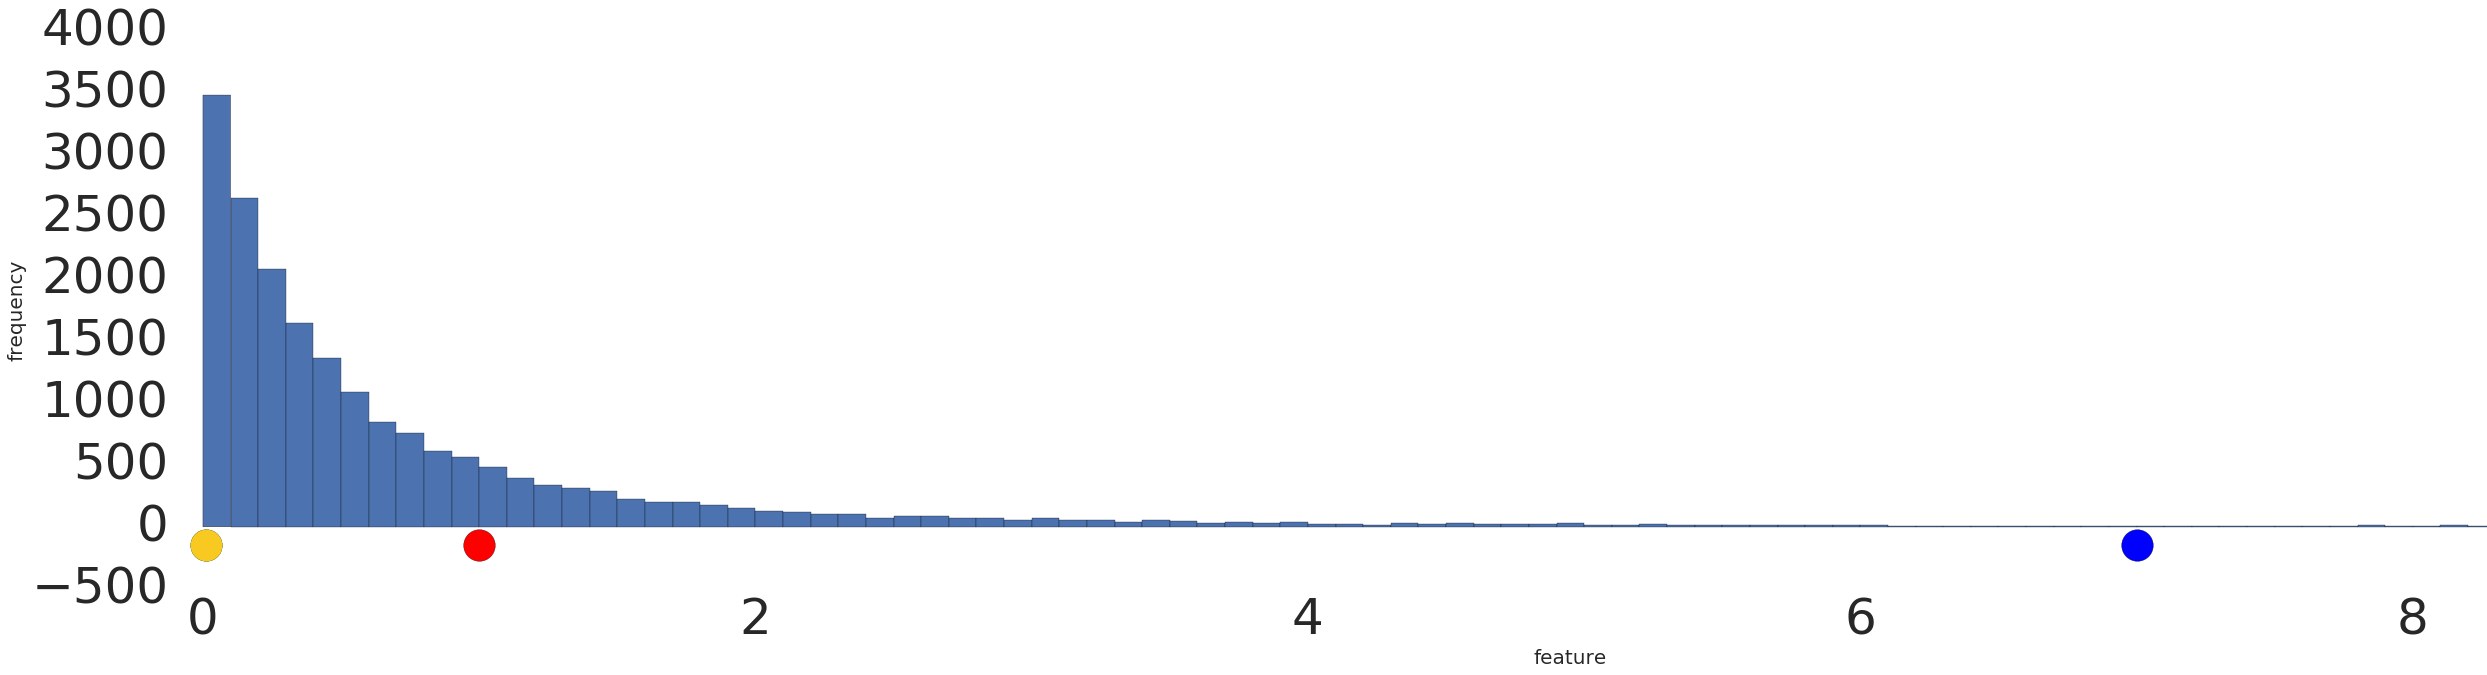
\includegraphics[width=8.0cm]{images/data_prep/scaling_distributions/LeftSkew.png}
					%\caption{Stripe Radar for Fraud Detection}
		\end{figure}
		
		Processiamo una distribuzione \textbf{power law} utilizzando una trasformazione logaritmica.
		Nella figura, la trasformazione logaritmica crea una distribuzione più uniforme. \textit{Notare la posizione dei punti tra prima e dopo}.
		% e il rosso è più vicino al blu che al giallo.
		
		\begin{figure}[!htbp]
			\centering
			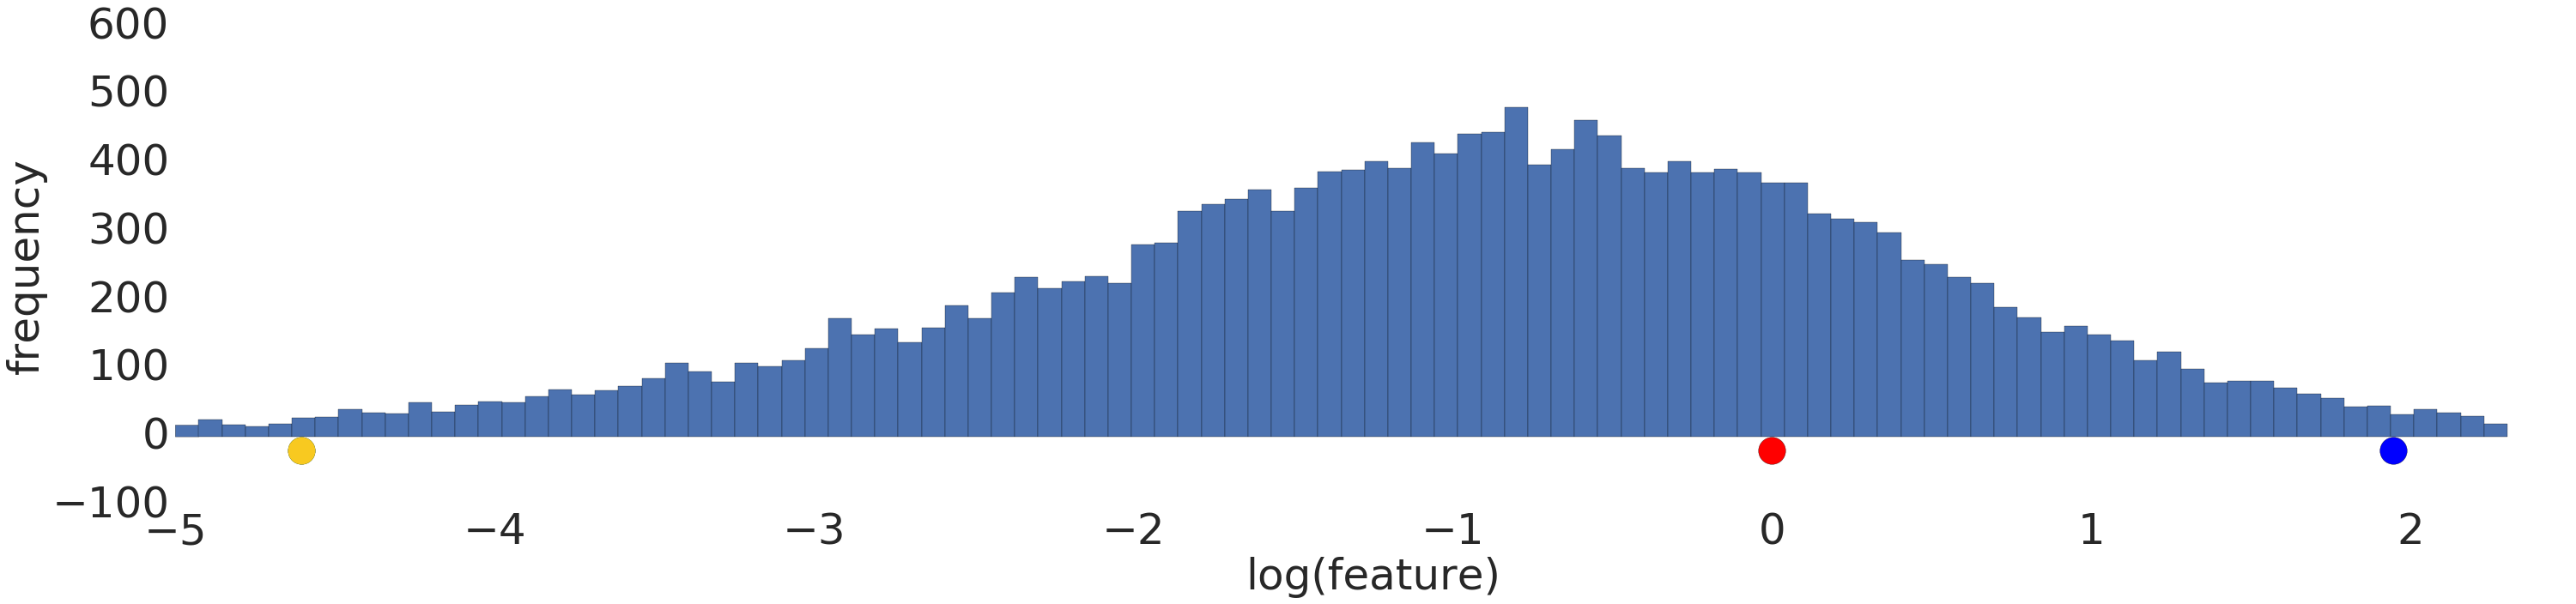
\includegraphics[width=8.0cm]{images/data_prep/scaling_distributions/NormalDistribution.png}
					%\caption{Stripe Radar for Fraud Detection}
		\end{figure}
	%\end{block}
	
\end{frame}

\subsubsection[Quantili]{Quantili}
\begin{frame}
	
	\frametitle{{\color{GradientDescentDiagramOrange}Trasformare le distribuzioni}: {\color{GradientDescentDiagramGreen}quantili}}
		
	%\begin{block}{}
		La normalizzazione e la log-transform riguardano distribuzioni di dati specifiche.\\
		Cosa succede se i dati non sono conformi a una distribuzione gaussiana o ad una legge di potenza?\\
		Esiste un \textbf{approccio generale} che si applica a qualsiasi distribuzione di dati? Proviamo a preprocessare questa distribuzione.
		
		\begin{figure}[!htbp]
			\centering
			\includegraphics[width=12.0cm]{images/data_prep/scaling_distributions/Preprocess.png}
					\caption{Una distribuzione non categorizzabile, \newline prima di aver applicato un qualunque preprocessing}
		\end{figure}
	%\end{block}
	
\end{frame}


\begin{frame}
	
	\frametitle{{\color{GradientDescentDiagramOrange}Trasformare le distribuzioni}: {\color{GradientDescentDiagramGreen}quantili}}
		
	%\begin{block}{}
		Intuitivamente, se i due esempi hanno solo pochi esempi tra loro, allora questi due esempi sono simili indipendentemente dai loro valori.\\
		Al contrario, se i due esempi hanno molti esempi tra loro, i due esempi sono meno simili.\\
		Pertanto, la \textbf{somiglianza} tra due esempi \textbf{diminuisce all'aumentare del numero di esempi tra di loro}.
		\newlinedouble
		Nè la normalizzazione (trasformazione lineare), nè una log-transform (in figura) riflettono questa intuizione sul funzionamento della somiglianza.
		\begin{figure}[!htbp]
			\centering
			\includegraphics[width=12.0cm]{images/data_prep/scaling_distributions/LogTransform.png}
					%\caption{Dopo aver applicato una log-transform}
		\end{figure}
	%\end{block}
	
\end{frame}


\begin{frame}
	
	\frametitle{{\color{GradientDescentDiagramOrange}Trasformare le distribuzioni}: {\color{GradientDescentDiagramGreen}quantili}}
		
	%\begin{block}{}
		Dividi i dati in intervalli, all'interno del quale ogni intervallo contiene un numero uguale di esempi.
		Questi confini degli intervalli sono detti \textbf{quantili}.\\
		Converti i tuoi dati in quantili eseguendo i seguenti passaggi:
		
		\begin{itemize}
			\item decidi il numero di intervalli
			\item definisci gli intervalli in modo tale che ogni intervallo abbia un numero uguale di esempi
			\item sostituisci ogni esempio con l'indice dell'intervallo al quale appartiene
			\item riporta gli indici allo stesso intervallo dei dati degli altri elementi scalando i valori dell'indice tra [0,1]
		\end{itemize}
		
		\begin{figure}[!htbp]
			\centering
			\includegraphics[width=12.0cm]{images/data_prep/scaling_distributions/Quantize.png}
					%\caption{Stripe Radar for Fraud Detection}
		\end{figure}
	%\end{block}
	
\end{frame}



\begin{frame}
	
	\frametitle{{\color{GradientDescentDiagramOrange}Trasformare le distribuzioni}: {\color{GradientDescentDiagramGreen}quantili}}
		
	%\begin{block}{}
		Dopo aver convertito i dati in quantili, la somiglianza tra due esempi è inversamente proporzionale al numero di esempi tra questi due esempi.
		\newlinedouble
		Oppure, matematicamente, dove se per $x$ intendiamo un qualsiasi esempio nel dataset: 
		\begin{itemize}
			\item $sim(A,B) \approx 1 - | \text{prob}[x > A] - \text{prob}[x > B] |$
			\item $sim(A,B) \approx 1 - | \text{quantile}(A) - \text{quantile}(B) |$
		\end{itemize}
		
		 I quantili sono la migliore scelta di default per trasformare i dati.\\
		 Tuttavia, per creare quantili che siano indicatori \textbf{affidabili} della distribuzione dei dati sottostanti, sono necessari \textbf{molti dati}.
		 \newlinedouble
		 Come regola pratica, per creare $n$ quantili, dovresti avere almeno $10n$ esempi. Se non disponi di dati sufficienti meglio applicare una semplice normalizzazione.
	%\end{block}
	
\end{frame}

\subsection[Creare proprie features]{Creare proprie features}

\begin{frame}
	
	\frametitle{{\color{GradientDescentDiagramRed}Creare proprie features}}

	%\begin{block}{}
		A volte i dati grezzi non dispongono delle feature sufficienti a svolgere operazioni di machine learning. In questi casi, vanno create delle nuove features. La \textbf{creazione di una feature} non significa creare dati dal nulla.
		\newlinedouble
		Per esempio, se state modellando il prezzo delle proprietà immobiliari, la superficie della proprietà ha ottime qualità predittive, perché le proprietà più grandi tendono a essere più costose; se invece della superficie fornite all’algoritmo di apprendimento la lunghezza dei lati della proprietà (le coordinate di latitudine e longitudine degli angoli), l’algoritmo potrebbe non saper che farsene delle informazioni che gli avete passato (almeno per la maggior parte degli algoritmi è così).
		\newlinedouble
		L'obiettivo è \textbf{creare nuove feature derivanti da quelle che già esistono} in modo che le nuove abbiano \textbf{capacità predittiva maggiore} rispetto a quelle originali (spesso implica conoscere bene il problema).
	%\end{block}
	
\end{frame}
}

\section[Apprendimento non supervisionato]{Apprendimento non supervisionato}
\sectionframe{images/covers/cover_unsupervised_fruit_market.jpg}{Apprendimento\\non supervisionato}

\subsection[Il Clustering]{Il Clustering}

\begin{frame}
	
	\frametitle{Apprendimento non supervisionato: il clustering}
	
	\begin{block}{Il clustering}
		Il \textbf{clustering} o \textbf{analisi dei gruppi} è un insieme di tecniche di analisi multivariata dei dati volte alla \textbf{selezione} e \textbf{raggruppamento} di \textbf{elementi omogenei} in un insieme di dati.
		\newlinedouble
		Le tecniche di clustering si basano su misure relative alla somiglianza tra gli elementi. In molti approcci questa similarità, o meglio, dissimilarità, è concepita in termini di \textbf{distanza in uno spazio multidimensionale}.
		\newlinedouble
		La bontà delle analisi ottenute dagli algoritmi di clustering dipende molto dalla scelta della \textbf{metrica}, e quindi da come è calcolata la distanza. Gli algoritmi di clustering raggruppano gli elementi sulla base della loro distanza reciproca, e quindi l'appartenenza o meno a un insieme dipende da quanto l'elemento preso in esame è distante dall'insieme stesso.
	\end{block}

\end{frame}


\subsubsection[Applicazioni Varie]{Applicazioni Varie}
\begin{frame}
	
	\frametitle{Il clustering: applicazioni}
	
	\begin{block}{Applicazioni Varie}
		Il clustering ha una miriade di utilizzi in una varietà di settori.\\
		Alcune \textbf{applicazioni comuni} per il clustering includono quanto segue:
		\begin{itemize}
			\item segmentazione del mercato
			\item customer profiling dei social network (individuando utenti simili)
			\item raggruppamento dei risultati di ricerca
			\item segmentazione delle immagini
			\item rilevamento delle anomalie (ad esempio, transazioni anomale)
		\end{itemize}
		
		Dopo la clusterizzazione, a ogni cluster viene assegnato un numero chiamato \textbf{cluster-ID}.
		%Ora puoi condensare l'intero set di funzionalità per un esempio nel suo ID cluster.\\
		Riuscire a rappresentare un esempio complesso mediante un semplice ID  rende il clustering uno strumento potente.
	\end{block}
		
\end{frame}


\begin{frame}
	
	\frametitle{Il clustering: applicazioni di supporto al Machine Learning}
	
	\begin{block}{Applicazioni di supporto}
		Estendendo l'idea, il clustering può semplificare datasets di grandi dimensioni.
		Alcune applicazioni di supporto al Machine Learning sono:
		\begin{itemize}
			\item \textbf{generalizzazione}: quando alcuni esempi in un cluster presentano features mancanti, è possibile ricavarli da altri esempi nel cluster
			\item \textbf{compressione}: le features degli esempi in un cluster possono essere sostituite dall'ID cluster pertinente. Questo semplifica le features e consente di risparmiare spazio di archiviazione.
			\item \textbf{privacy}: è possibile preservare la privacy raggruppando gli utenti e associando i dati degli utenti ad un cluster-ID invece che a utenti specifici. Per garantire che non sia possibile associare i dati utente a un utente specifico, il cluster deve raggruppare un numero sufficiente di utenti
		\end{itemize}
	\end{block}
	
\end{frame}
\subsection[Image Segmentation]{Image Segmentation}
%\begin{frame}
%
%	\frametitle{Il Clustering nella segmentazione delle immagini}
%
%	\begin{block}{Clustering}
%		Come già detto lo scopo del clustering è rilevare i gruppi naturali (cluster) nei dati:
%
%		\begin{itemize}
%			\item naturale significa che i gruppi dovrebbero corrispondere a qualche interpretazione umana
%			\item ogni cluster deve essere composto da punti per i quali la similarità agli altri punti all'interno di dello stesso cluster è superiore alla similarità rispetto a punti appartenenti ad altri clusters
%			\item questo pone il problema di come misurare la similarità tra punti e, eventualmente, tra cluster
%			\item diverse misure di similarità producono differenti risultati di clusterizzazione
%		\end{itemize}
%	\end{block}
%
%\end{frame}


\begin{frame}

	\frametitle{Il clustering: segmentazione delle immagini}

%	\begin{block}{}
		Come detto, una delle applicazioni più comuni del clustering è la \textbf{segmentazione delle immagini}.
		\newlinedouble
		Questo ambito ci aiuterà molto soprattutto per facilitare la trattazione delle varie tecniche e poter avere un riscontro/confronto visivo diretto tra le varie tecniche di clusterizazzione.
		\begin{itemize}
			\item una volta completato il clustering, ogni cluster viene associato con una label (o un ID) e la posizione del centro del cluster nello spazio delle caratteristiche
			\item la segmentazione dell'immagine si ottiene associando ad ogni pixel dell'immagine l'etichetta (o il centro) del cluster a cui appartiene nello spazio delle features
			\item sono state proposte diverse tecniche di clustering. Dato un dataset, diverse tecniche di clustering possono produrre risultati differenti
		\end{itemize}
%	\end{block}

\end{frame}


\begin{frame}

	\frametitle{Il clustering: segmentazione delle immagini}

%	\begin{block}{}

		\begin{columns}

			\column{0.5\linewidth}
			\begin{itemize}
				\item si noti che un cluster non corrisponde necessariamente a una regione dell'immagine
				\item una regione percettivamente saliente può essere costituita da più cluster o più regioni
				\ifthenelse{\boolean{highschool}}{}{
					\item potrebbe essere necessario decidere qual è il migliore
					\item a tal fine è necessaria una certa misura della qualità del clustering
				}
			\end{itemize}

			\column{0.5\linewidth}
			\begin{figure}[!htbp]
				\centering
				\includegraphics[width=6.0cm]{images/unsupervised/image_segmentation/image_segmentation.png}
				%\caption{ENEL QQ-Plot Normale}
				%\label{Enel_QQ_Plot_Normal}
			\end{figure}

		\end{columns}

%	\end{block}

\end{frame}


\ifthenelse{\boolean{highschool}}{}{
	\begin{frame}
	
		\frametitle{Il clustering: segmentazione delle immagini}
	
		%	\begin{block}{}
	
				Una \textbf{misura quantitativa della qualità dei risultati} del clustering è la distanza media dei punti del cluster dal loro centro del cluster.
	
				\begin{empheq}[box=\fcolorbox{blue!40!black!60}{yellow!10}]{align*}
					\mathbf{J} = \frac{1}{N} \sum_{i=1}^{N}\sum_{k=1}^{K}r_{ik} \Vert x_i-\mu_k\Vert^2
				\end{empheq}
				Dove:
				\begin{itemize}
					\item $x_i\text{ }i=1,...,N$ i punti del dataset (data point)
					\item $\mu_k\text{ }k=1,...,K$ i centri dei clusters
					\item $r_{ik}$ un indicatore binario che vale:
					\begin{itemize}
						\item[--] 1 se il punto $x_i$ appartiene al cluster $k$ con centro $\mu_k$
						\item[--] 0 altrimenti
					\end{itemize}
				\end{itemize}
		%	\end{block}
	
	\end{frame}
	
	
	\begin{frame}
	
		\frametitle{Il clustering: segmentazione delle immagini}
	
		%	\begin{block}{}
				\begin{empheq}[box=\fcolorbox{blue!40!black!60}{yellow!10}]{align*}
					\mathbf{J} = \frac{1}{N} \sum_{i=1}^{N}\sum_{k=1}^{K}r_{ik} \Vert x_i-\mu_k\Vert^2
				\end{empheq}
				Va osservato che il valore di $\mathbf{J}$ può essere utilizzato per confrontare i risultati del clustering a condizione che il numero di cluster $K$ sia lo stesso:
				\begin{itemize}
					\item il valore di $\mathbf{J}$ non può essere utilizzato per confrontare due risultati di clustering se sono stati costruiti con un numero di clusters $K$ diverso
				\end{itemize}
				Infatti, se il valore di $K$ non fosse vincolato, il clustering ottimale risulterebbe nella soluzione banale:
				\begin{itemize}
					\item ogni punto del dataset definisce un cluster, $K = N$, $J = 0$
				\end{itemize}
		%	\end{block}
	
	\end{frame}
	
	\begin{frame}
	
		\frametitle{Il clustering: segmentazione delle immagini}
	
		%	\begin{block}{}
			La scelta del numero dei cluster $K$ è un problema impegnativo.\\
			La scelta ottimale di $K$ dovrebbe essere un compromesso tra:
			\begin{itemize}
				\item la massima compressione dei dati, ottenuta utilizzando un singolo cluster
				\item la massima accuratezza ottenuta definendo un cluster per ogni data point
			\end{itemize}
			Quando il numero di cluster $K$ non è noto in anticipo, è necessario considerare alcune misure della qualità del clustering per diversi valori $K$ e si seleziona il valore di $K$ per massimizzare questa misura di qualità
		%	\end{block}
	
	\end{frame}
}

\subsection[Tipologie di Clustering]{Tipologie di Clustering}

\ifthenelse{\boolean{highschool}}{}{
	\begin{frame}
		
		\frametitle{Algoritmi di Clustering: le varie tipologie}
		
		%\begin{block}{}
			Quando si sceglie un algoritmo di clustering, è necessario considerare se l'algoritmo si adatta al proprio dataset.
			I dataset nell'apprendimento automatico possono avere milioni di esempi, ma non tutti gli algoritmi di clustering scalano in modo efficiente.
			\newlinedouble
			Molti algoritmi di clustering funzionano calcolando la \textbf{somiglianza tra tutte le coppie} di esempi. Ciò significa che il loro tempo di esecuzione aumenta al quadrato del numero di esempi n. Questi algoritmi, con \textbf{complessità $\boldsymbol{O(n^2)}$}, non sono pratici quando il numero di esempi è in milioni.
			\newlinedouble
			Un buon compromesso può essere ottenuto tramite l'algoritmo \textbf{K-means}, che ha una \textbf{complessità $\boldsymbol{O(n)}$}, il che significa che l'algoritmo scala linearmente con $n$.
		%\end{block}

	\end{frame}
}

\begin{frame}
	
	\frametitle{Algoritmi di Clustering: le varie tipologie}
	
	%\begin{block}{}
		È possibile distinguere diverse tipologie di clustering:
		\begin{itemize}
			\item {\color{GradientDescentDiagramBlue}Centroid-based Clustering}
			\item {\color{GradientDescentDiagramGreen}Hierarchical Clustering}
			\item {\color{GradientDescentDiagramOrange}Distribution-based Clustering}
			\item {\color{GradientDescentDiagramRed}Density-based Clustering}
		\end{itemize}
		\vspace{4mm}
		Per una lista completa leggere:\\
		\underline{\href{https://link.springer.com/article/10.1007/s40745-015-0040-1}{A Comprehensive Survey of Clustering Algorithms}}\\
		Xu, D. \& Tian, Y. Ann. Data. Sci. (2015) 2: 165
	%\end{block}
	
\end{frame}



\subsubsection[Centroid-based (K-means)]{Centroid-based \textit{(K-means)}}
\begin{frame}

	\frametitle{{\color{GradientDescentDiagramBlue}Centroid-based Clustering}, in sintesi}

	%\begin{block}{}
		Il \textbf{centroid-based clustering} organizza i dati in cluster non gerarchici, in contrasto con il clustering gerarchico definito in seguito. \textbf{K-means} è l'algoritmo di clustering basato su centroidi più utilizzato.
		\newlinedouble
		Gli algoritmi basati su centroidi sono efficienti ma \textbf{sensibili} alle \textbf{condizioni iniziali} e ai \textbf{valori anomali}.

		\begin{figure}[!htbp]
			\centering
			\includegraphics[width=5.0cm]{images/unsupervised/types/Clustering_CentroidBased.pdf}
					%\caption{Stripe Radar for Fraud Detection}
		\end{figure}
	%\end{block}

\end{frame}



\begin{frame}

	\frametitle{{\color{GradientDescentDiagramBlue}Centroid-based Clustering}: il K-means}

	\begin{scriptsize}
	\begin{block}{Come calcolare la media $\mu$ per un insieme di punti $\in \mathbb{R}^1$}
		\begin{figure}[!htbp]
			\centering
			\includegraphics<1>[width=0.7\linewidth]{images/unsupervised/kmeans/mean_r1.png}
			\includegraphics<2>[width=0.7\linewidth]{images/unsupervised/kmeans/mean_r1_mean.png}
					%\caption{Stripe Radar for Fraud Detection}
		\end{figure}
		
		\begin{itemize}
	        \item<1-> $\mu = \frac{2+3+7+8}{4} = 5$	       
	        \item<2-> $\mu = \frac{x_1 + x_2 + ... + x_N}{N} = \frac{1}{N}\sum_{i=1}^{N} x_i$
	    \end{itemize}

	\end{block}
	\end{scriptsize}
	
\end{frame}

\begin{frame}

	\frametitle{{\color{GradientDescentDiagramBlue}Centroid-based Clustering}: il K-means}

	\begin{scriptsize}
	\begin{block}{Come calcolare la media $\mu$ per un insieme di punti $\in \mathbb{R}^2$}
		\begin{figure}[!htbp]
			\centering
			\includegraphics<1>[width=0.56\linewidth]{images/unsupervised/kmeans/mean_r2.png}
			\includegraphics<2>[width=0.56\linewidth]{images/unsupervised/kmeans/mean_r2_mean.png}
					%\caption{Stripe Radar for Fraud Detection}
		\end{figure}
		
		\begin{align}
			\bar \mu = (\mu_1, \mu_2) &= \left(\frac{2+3+7+8}{4}, \frac{1+0+1+2}{4}\right) = (5,1)\nonumber \\
			\bar \mu = (\mu_1, \mu_2) &= \frac{1}{4} \left[(2,1) + (3,0) + (7,1) + (8,2)\right] \nonumber \\
			& = \frac{1}{4} (20, 4) \nonumber \\
			& = (5,1) \nonumber
		\end{align}
	\end{block}
	\end{scriptsize}
	
\end{frame}


\begin{frame}

	\frametitle{{\color{GradientDescentDiagramBlue}Centroid-based Clustering}: il K-means}
	
	\begin{scriptsize}
	\begin{block}{Come calcolare la media $\mu$ per un insieme di punti $\in \mathbb{R}^2$}
		\begin{figure}[!htbp]
			\centering
			\includegraphics[width=0.5\linewidth]{images/unsupervised/kmeans/mean_r2_mean.png}
					%\caption{Stripe Radar for Fraud Detection}
		\end{figure}
		
		$$\bar \mu = (\mu_1, \mu_2) = \frac{1}{N} (\bar x_1 + \bar x_2 + ... + \bar x_N) = \frac{1}{N}\sum_{i=1}^{N} \bar x_i$$

	\end{block}
	
	\begin{block}{Come calcolare la media $\mu$ per un insieme di punti $\in \mathbb{R}^D$}
		$$\bar \mu = (\mu_1, \mu_2, ..., \mu_D) = \frac{1}{N} (\bar x_1 + \bar x_2 + ... + \bar x_N) = \frac{1}{N}\sum_{i=1}^{N} \bar x_i$$
	\end{block}
	\end{scriptsize}

\end{frame}




\begin{frame}

	\frametitle{{\color{GradientDescentDiagramBlue}Centroid-based Clustering}: il K-means}

	%\begin{block}{}
		Il clustering \textbf{K-means} è caratterizzato dai seguenti aspetti chiave:
		\begin{itemize}
			\item con il clustering K-means, il \textbf{numero K} di cluster deve essere specificato prima di iniziare il processo di clustering
			\item il clustering K-means \textbf{non è gerarchico}: il dataset è semplicemente partizionato in \textbf{K gruppi disgiunti}
			\ifthenelse{\boolean{highschool}}{}{
				\item K-means scala come $O(nk)$, dove $k$ è il numero di clusters e $n$ la dimensione del dataset
			}
		\end{itemize}
		
		\pause
		\vspace{2em}
		Definiamo la variabile binaria $r_{ik}$ che vale:
		\begin{itemize}
			\item 1: se l'$i$-esima osservazione $\in$ al cluster $k$
			\item 0: altrimenti
		\end{itemize}
		Ogni osservazione può essere assegnata ad un solo cluster, di conseguenza per ogni singola osservazione $i$ esisterà una e una sola $\hat{k}$ per il quale vale che  $r_{i\hat{k}}=1$.

	%\end{block}

\end{frame}



\begin{frame}

	\frametitle{{\color{GradientDescentDiagramBlue}Centroid-based Clustering}: il K-means}

	\begin{block}{K-means: algoritmo}
		\begin{enumerate}
			\item inizializza in modo casuale i valori delle variabili binarie $r_{ik}$ in modo che ogni punto sia assegnato casualmente ad un solo cluster 
			\item calcola la media di ogni cluster (cioè il centro del cluster):\\
				$\mu_k = \frac{\sum_{i=1}^{N}r_{ik}x_i}{\sum_{i=1}^{N}r_{ik}} =$ (la media delle osservazioni appartenti al cluster $k$)
			\item aggiorna i valori delle variabili binarie $r_{ik}$, in modo che ogni punto sia assegnato al centro del cluster più vicino
			\item se nessuna variabile viene aggiornata nel passaggio precedente, fermarsi, altrimenti tornare al passaggio 2
		\end{enumerate}
		\vspace{2mm}
		Una possibile inizializzazione alternativa prevede di fissare direttamente i centri dei clusters randomicamente (ad esempio scegliendo $k$ distinti punti random dal dataset) e poi procedere dal punto 3
	\end{block}

\end{frame}


\begin{frame}

	\frametitle{{\color{GradientDescentDiagramBlue}Centroid-based Clustering}: il K-means}

	\begin{block}{K-means: algoritmo}
		\begin{figure}[!htbp]
			\centering
			\includegraphics[width=1.0\linewidth]{images/unsupervised/kmeans/kmeans_algorithm.png}
					%\caption{Stripe Radar for Fraud Detection}
		\end{figure}
	\end{block}

\end{frame}


%\begin{frame}
%
%	\frametitle{{\color{GradientDescentDiagramBlue}Centroid-based Clustering}: il K-means}
%
%	\begin{block}{K-means: algoritmo\\Inizializzazione alternativa}
%		\begin{figure}[!htbp]
%			\centering
%			\includegraphics[width=5.75cm]{images/unsupervised/kmeans/kmeans_step_1.png}
%					%\caption{Stripe Radar for Fraud Detection}
%		\end{figure}
%	\end{block}
%
%\end{frame}
%
%
%\begin{frame}
%
%	\frametitle{{\color{GradientDescentDiagramBlue}Centroid-based Clustering}: il K-means}
%
%	\begin{block}{K-means: algoritmo\\Aggiorno gli $r_{ik}\text{ }$(punto 3)}
%		\begin{figure}[!htbp]
%			\centering
%			\includegraphics[width=5.75cm]{images/unsupervised/kmeans/kmeans_step_2.png}
%					%\caption{Stripe Radar for Fraud Detection}
%		\end{figure}
%	\end{block}
%
%\end{frame}
%
%
%\begin{frame}
%
%	\frametitle{{\color{GradientDescentDiagramBlue}Centroid-based Clustering}: il K-means}
%
%	\begin{block}{K-means: algoritmo\\La condizione di stop non è ancora rispettata quindi aggiorno i $\mu_k$ (punto 2)}
%		\begin{figure}[!htbp]
%			\centering
%			\includegraphics[width=5.75cm]{images/unsupervised/kmeans/kmeans_step_3.png}
%					%\caption{Stripe Radar for Fraud Detection}
%		\end{figure}
%	\end{block}
%
%\end{frame}
%
%
%\begin{frame}
%
%	\frametitle{{\color{GradientDescentDiagramBlue}Centroid-based Clustering}: il K-means}
%
%	\begin{block}{K-means: algoritmo\\Aggiorno gli $r_{ik}\text{ }$(punto 3)}
%		\begin{figure}[!htbp]
%			\centering
%			\includegraphics[width=5.75cm]{images/unsupervised/kmeans/kmeans_step_4.png}
%					%\caption{Stripe Radar for Fraud Detection}
%		\end{figure}
%	\end{block}
%
%\end{frame}


\begin{frame}

	\frametitle{{\color{GradientDescentDiagramBlue}Centroid-based Clustering}: il K-means}

%	\begin{block}{K-means: algoritmo}
		\centering
		\animategraphics[controls={play, step, stop}, height=7cm]{20.0}{images/unsupervised/kmeans/k_means_1/k_means_1-}{0}{242}
%	\end{block}

\end{frame}


\begin{frame}

	\frametitle{{\color{GradientDescentDiagramBlue}Centroid-based Clustering}: il K-means}

%	\begin{block}{K-means: algoritmo}
		\centering
		\animategraphics[controls={play, step, stop}, height=7cm]{3.0}{images/unsupervised/kmeans/k_means_2/k_means_2-}{0}{14}
%	\end{block}

\end{frame}


\begin{frame}

	\frametitle{{\color{GradientDescentDiagramBlue}Centroid-based Clustering}: il K-means}

%	\begin{block}{K-means: algoritmo}
		\centering
		\animategraphics[controls={play, step, stop}, height=7cm]{3.0}{images/unsupervised/kmeans/k_means_3/k_means_3-}{0}{12}
%	\end{block}

\end{frame}


\begin{frame}

	\frametitle{{\color{GradientDescentDiagramBlue}Centroid-based Clustering}: il K-means}

	\begin{block}{}
		Per altri esempi interattivi:\\
		\begin{itemize}
			\item \underline{\href{https://stanford.edu/class/engr108/visualizations/kmeans/kmeans.html}{Esempio 1}}
			\item \underline{\href{http://alekseynp.com/viz/k-means.html}{Esempio 2}}
		\end{itemize}
	\end{block}

\end{frame}


\ifthenelse{\boolean{highschool}}{}{
	\begin{frame}
	
		\frametitle{{\color{GradientDescentDiagramBlue}Centroid-based Clustering}: il K-means}
	
		\begin{block}{K-means: dimostrazione matematica parte 1}
			Ricordiamo l'espressione di:
			\begin{empheq}[box=\fcolorbox{blue!40!black!60}{yellow!10}]{align*}
				\mathbf{J} = \frac{1}{N} \sum_{i=1}^{N}\sum_{k=1}^{K}r_{ik} \Vert x_i-\mu_k\Vert^2
			\end{empheq}
	
			Dati $N$ esempi assegnati a $K$ cluster, minimizziamo la somma delle distanze degli esempi rispetto ai loro centroidi. Dove:
			\begin{itemize}
				\item $r_{ik}=1$ quando l'$i$-esimo esempio è assegnato al $k$-esimo cluster, $=0$ altrimenti
				\item $\mu_k$ è il centroide del $k$-esimo cluster
			\end{itemize}
		\end{block}
	
	\end{frame}
	
	
	\begin{frame}
	
		\frametitle{{\color{GradientDescentDiagramBlue}Centroid-based Clustering}: il K-means}
	
		\begin{block}{K-means: dimostrazione matematica parte 2}
	
			Vogliamo quindi minimizzare la seguente espressione:
			$$\underset{r,\mu}{min}\sum_{i=1}^{N}\sum_{k=1}^{K}r_{ik} \Vert x_i-\mu_k\Vert^2$$
			dove:
			$$r_{ik} \in \{0,1\}\quad\forall i,k$$
			e
			$$\sum^{K}_{k=1}r_{ik}=1\quad\forall i$$
	
			Per minimizzare l'espressione rispetto al cluster con centroide $\mu_k$, deriviamo rispetto a $\mu_k$ e la uguagliamo a 0.
		\end{block}
	
	\end{frame}
	
	
	\begin{frame}
	
		\frametitle{{\color{GradientDescentDiagramBlue}Centroid-based Clustering}: il K-means}
	
		\begin{block}{K-means: dimostrazione matematica parte 3}
			
			\begin{center}
				$f(\mu) = \sum^{N}_{i=1} \sum_{k=1}^{K} r_{ik} ||x_i - \mu_k||^2$ \newlinedouble %\hline
				$\frac{\partial f}{\partial \mu_k} = 2 \sum_{i=1}^{N} r_{ik}(x_i - \mu_k) = 0$  \\~\\ $\pmb{\Downarrow}$ \\~\\
				 %\hline
				$\quad \sum_{i=1}^{N} r_{ik}\mu_{k} = \sum_{i=1}^{N} r_{ik}x_{i}$ \newlinedouble %\hline
				$\mu_k \sum_{i=1}^{N} r_{ik} = \sum_{i=1}^{N} r_{ik} x_i$ \newlinedouble %\hline
				$\mu_k = \frac{\sum_{i=1}^{N} r_{ik} x_i}{\sum_{i=1}^{N} r_{ik}}$	
			\end{center}
	
		\end{block}
	
	\end{frame}
	
	
	\begin{frame}
	
		\frametitle{{\color{GradientDescentDiagramBlue}Centroid-based Clustering}: il K-means}
	
		\begin{block}{K-means: dimostrazione matematica parte 4}
	
	%		\begin{scriptsize}
				\begin{gather*}
					 \mu_k = \frac{\sum_{i=1}^{N} r_{ik} x_i}{\sum_{i=1}^{N} r_{ik}}
				\end{gather*}
	%		\end{scriptsize}
	
			\begin{itemize}
				\item il \textbf{numeratore} è la somma di tutti i  punti (vettori) appartenti al cluster
				\item il \textbf{denominatore} è il numero di esempi nel cluster
				\item pertanto, il centroide del cluster $\mu_k$ è la media delle posizioni dei punti appartenenti al cluster
				\item quindi in estrema sintesi: per minimizzare $J$ è sufficiente aggiornare il $\mu_k$ del cluster sommando i vari vettori (punti) del cluster e dividere per il numero di elementi del cluster (media di tutti i punti nel cluster)
			\end{itemize}
	
		\end{block}
	
	\end{frame}
}


\begin{frame}

	\frametitle{{\color{GradientDescentDiagramBlue}Centroid-based Clustering}: il K-means}

	\begin{block}{K-means: svantaggi}
		\begin{itemize}
			\item uno svantaggio del clustering k-means è che non è garantito che converga sempre allo stesso clustering
				\begin{itemize}
					\item[--] l'esecuzione della procedura più volte può produrre cluster diversi: a seconda dell'inizializzazione randomica l'algoritmo può convergere a minimi (locali) diversi
				\end{itemize}
			\item un altro svantaggio è che l'uso della distanza euclidea determina cluster sferici
		\end{itemize}
	\end{block}

\end{frame}


\begin{frame}

	\frametitle{{\color{GradientDescentDiagramBlue}Centroid-based Clustering}: il K-means}

	\begin{block}{K-means: minimi locali diversi parte 1}
		\begin{itemize}
			\item Considera il seguente dataset composto da punti 2D appartenenti a 2 classi distinte
			\item ogni classe è caratterizzata da una distribuzione gaussiana (parzialmente sovrapposta)
		\end{itemize}

		\begin{figure}[!htbp]
			\centering
			\includegraphics[width=4.50cm]{images/unsupervised/kmeans/highley_gt.png}
					%\caption{Stripe Radar for Fraud Detection}
		\end{figure}
	\end{block}

\end{frame}


\begin{frame}

	\frametitle{{\color{GradientDescentDiagramBlue}Centroid-based Clustering}: il K-means}

	\begin{block}{K-means: minimi locali diversi parte 2}
		Risultato usando K-means con $K=2$
		\begin{columns}
			\column{0.5\linewidth}
			\begin{figure}[!htbp]
				\centering
				\includegraphics[angle=0,width=1\linewidth]{images/unsupervised/kmeans/highley_gt.png}
%				\caption{Single-Link Good K}
				%\label{Enel_HistFit_Normal}
			\end{figure}

			\column{0.5\linewidth}
			\begin{figure}[!htbp]
				\centering
				\includegraphics[angle=0,width=1\linewidth]{images/unsupervised/kmeans/highley_2k.png}
%				\caption{Single-Link Dendogram Good K}
				%\label{Enel_QQ_Plot_Normal}
			\end{figure}

		\end{columns}
	\end{block}

\end{frame}



\begin{frame}

	\frametitle{{\color{GradientDescentDiagramBlue}Centroid-based Clustering}: il K-means}

	\begin{block}{K-means: minimi locali diversi parte 3}
		Risultato 1 usando K-means con $K=3$
		\begin{columns}
			\column{0.5\linewidth}
			\begin{figure}[!htbp]
				\centering
				\includegraphics[angle=0,width=1\linewidth]{images/unsupervised/kmeans/highley_gt.png}
%				\caption{Single-Link Good K}
				%\label{Enel_HistFit_Normal}
			\end{figure}

			\column{0.5\linewidth}
			\begin{figure}[!htbp]
				\centering
				\includegraphics[angle=0,width=1\linewidth]{images/unsupervised/kmeans/highley_3k_1.png}
%				\caption{Single-Link Dendogram Good K}
				%\label{Enel_QQ_Plot_Normal}
			\end{figure}

		\end{columns}
	\end{block}

\end{frame}


\begin{frame}

	\frametitle{{\color{GradientDescentDiagramBlue}Centroid-based Clustering}: il K-means}

	\begin{block}{K-means: minimi locali diversi parte 4}
		Risultato 2 usando K-means con $K=3$
		\begin{columns}
			\column{0.5\linewidth}
			\begin{figure}[!htbp]
				\centering
				\includegraphics[angle=0,width=1\linewidth]{images/unsupervised/kmeans/highley_gt.png}
%				\caption{Single-Link Good K}
				%\label{Enel_HistFit_Normal}
			\end{figure}

			\column{0.5\linewidth}
			\begin{figure}[!htbp]
				\centering
				\includegraphics[angle=0,width=1\linewidth]{images/unsupervised/kmeans/highley_3k_2.png}
%				\caption{Single-Link Dendogram Good K}
				%\label{Enel_QQ_Plot_Normal}
			\end{figure}

		\end{columns}
	\end{block}

\end{frame}


\begin{frame}

	\frametitle{{\color{GradientDescentDiagramBlue}Centroid-based Clustering}: considerazioni}

	%\begin{block}{K-means: considerazioni}

		\begin{itemize}
			\item La procedura iterativa K-means cerca di spostare i centri del cluster in modo da farli corrispondere a posizioni nello spazio delle features in cui si concentrano molti punti
				\begin{itemize}
					\item[--] idealmente, i centri dei cluster dovrebbero essere posizionati in corrispondenza dei \textbf{picchi della densità} di distribuzione dei dati nello spazio delle features
				\end{itemize}
			\item Un risultato dell'utilizzo della distanza euclidea per valutare la vicinanza di un punto dati al centro del suo cluster è che la forma di ciascun cluster rappresenta una cella Voronoi
				\begin{itemize}
					\item[--] l'insieme di tutti i cluster determina una \textbf{tassellazione Voronoi} del spazio delle caratteristiche
				\end{itemize}
		\end{itemize}

		\begin{figure}[!htbp]
				\centering
				\includegraphics[angle=0,width=0.18\linewidth]{images/unsupervised/kmeans/kmeans_voronoi.png}
%				\caption{Single-Link Dendogram Good K}
				%\label{Enel_QQ_Plot_Normal}
			\end{figure}
	%\end{block}

\end{frame}


\begin{frame}

	\frametitle{{\color{GradientDescentDiagramBlue}Centroid-based Clustering}: segmentazione con il K-means}

%	\begin{block}{K-means: considerazioni}
		\begin{figure}[!htbp]
			\centering
			\includegraphics[angle=0,width=0.8\linewidth]{images/unsupervised/kmeans/kmeans_lion.pdf}
%				\caption{Single-Link Dendogram Good K}
			%\label{Enel_QQ_Plot_Normal}
		\end{figure}
%	\end{block}

\end{frame}


\begin{frame}

	\frametitle{{\color{GradientDescentDiagramBlue}Centroid-based Clustering}: segmentazione con il K-means}

%	\begin{block}{K-means: considerazioni}
		\begin{figure}[!htbp]
				\centering
				\includegraphics[angle=0,width=0.85\linewidth]{images/unsupervised/kmeans/kmeans_pots.pdf}
%				\caption{Single-Link Dendogram Good K}
				%\label{Enel_QQ_Plot_Normal}
			\end{figure}
%	\end{block}

\end{frame}


\subsubsection[Hierarchical (AGNES e DIANA)]{Hierarchical \textit{(AGNES e DIANA)}}
\begin{frame}

	\frametitle{{\color{GradientDescentDiagramGreen}Hierarchical Clustering}, in sintesi}

	%\begin{block}{}
		Il clustering gerarchico crea un albero di clusters.\\
		È una metodologia di clustering che cerca di costruire una gerarchia di cluster, rappresentata con un albero che prende il nome di \emph{dendogramma}.\newlinedouble
		%Mira a creare una sorta di tassonomia al variare del numero di clusters $K$.\\ %  da $1$ a $N$ dove $N$ è il numero di osservazioni del dataset.
		È possibile decidere un numero $K$ qualsiasi di clusters per il nostro specifico problema tagliando l'albero costruito con tale procedura al giusto livello.
		\begin{figure}[!htbp]
			\centering
			\includegraphics[width=7.0cm]{images/unsupervised/types/Clustering_Hierarchical.pdf}
					%\caption{Stripe Radar for Fraud Detection}
		\end{figure}
	%\end{block}

\end{frame}


\begin{frame}

	\frametitle{{\color{GradientDescentDiagramGreen}Hierarchical Clustering}}

%	\begin{block}{Idea di base}
		Il clustering gerarchico può essere suddiviso in due tipologie principali:
		\begin{itemize}
			\item \textbf{clustering gerarchico agglomerativo}: è noto anche come \textbf{AGNES} (Agglomerative Nesting, bottom-up). Cioè, ogni oggetto viene inizialmente considerato come un cluster a elemento singolo (foglia). Ad ogni passaggio dell'algoritmo, i due cluster più simili vengono combinati in un nuovo cluster più grande (nodi). Questa procedura viene ripetuta finché tutti i punti non sono membri di un unico grande cluster (radice). Il risultato è un albero che può essere tracciato come un dendrogramma.
			\item \textbf{clustering gerarchico divisivo}: è noto anche come \textbf{DIANA} (Divise Analysis, top-down). L'algoritmo procede in ordine inverso rispetto all'AGNES. Inizia con la radice, in cui tutti gli oggetti sono inclusi in un singolo cluster. In ogni fase dell'iterazione, il cluster più eterogeneo viene diviso in due. Il processo viene iterato fino a quando tutti gli oggetti si trovano nel loro proprio cluster.
		\end{itemize}
%	\end{block}
\end{frame}


\begin{frame}

	\frametitle{{\color{GradientDescentDiagramGreen}Hierarchical Clustering}}

%	\begin{block}{Idea di base}
		\ifthenelse{\boolean{highschool}}{}{Si noti che il clustering agglomerativo è utile per identificare piccoli cluster. Il clustering divisivo è utile per identificare cluster di grandi dimensioni.}
		\begin{figure}[!htbp]
			\centering
			\includegraphics[width=12.0cm]{images/unsupervised/hierarchical/hierarchical-clustering-agnes-diana.png}
					%\caption{Stripe Radar for Fraud Detection}
		\end{figure}

%	\end{block}
\end{frame}



\begin{frame}

	\frametitle{{\color{GradientDescentDiagramGreen}Hierarchical Clustering}}

	\begin{block}{Clustering gerarchico agglomerativo: idea di base}
		\begin{itemize}
			\item agglomerare ricorsivamente i punti in cluster combinando i punti e i cluster più vicini per ottenere cluster più grandi fino a quando tutti i punti vengono raccolti in un solo cluster
		\end{itemize}
		Il processo ricorsivo definisce una gerarchia che rende esplicita la struttura del set di dati in termini di cluster di grandi dimensioni e sub-clusters.
		\newlinedouble
		Il clustering gerarchico richiede la specifica di come calcolare la distanza tra:
		\begin{itemize}
			\item due punti (Manhattan, Euclidean, cosine ...)
			\item un punto e un cluster (...)
			\item due cluster (...)
		\end{itemize}
	\end{block}

\end{frame}


\begin{frame}

	\frametitle{{\color{GradientDescentDiagramGreen}Hierarchical Clustering}}

	\begin{block}{Clustering gerarchico agglomerativo: algoritmo}
		\begin{enumerate}
			\item all'inizio, ogni punto definisce un nuovo cluster, risultando in N cluster ciascuno contenente un solo punto. Le distanze tra tutte le coppie di cluster vengono calcolate e memorizzate in una matrice $A_{NN}$
			\item trovare la coppia di cluster più vicina e unirli in un unico cluster. Calcola e memorizza la distanza tra il nuovo cluster e tutti gli altri (ovvero, aggiorna $A_{NN}$)
			\item ripeti il passaggio 2 fino a quando tutti i punti sono raggruppati in un unico cluster composto da $N$ punti
		\end{enumerate}
	\end{block}

\end{frame}


\begin{frame}

	\frametitle{{\color{GradientDescentDiagramGreen}Hierarchical Clustering}}

	\begin{block}{Metriche di dissimilarità più utilizzate: (indicate successivamente con $\bigstar$)}

		\begin{itemize}
			\item \textbf{Euclidean distance}:\\
				\makebox[\textwidth]{$d_{euc}(x,y) = \sqrt{\sum^n_{i=1}(x_i - y_i)^2}$}
			\item \textbf{Manhattan distance}:\\
				\makebox[\textwidth]{$d_{man}(x,y) = \sum^n_{i=1}|(x_i - y_i)|$}
			\item \textbf{Pearson correlation distance}:\\
				\makebox[\textwidth]{$d_{cor}(x, y) = 1 - \frac{\sum^n_{i=1}(x_i-\bar x)(y_i - \bar y)}{\sqrt{\sum^n_{i=1}(x_i-\bar x)^2\sum^n_{i=1}(y_i - \bar y)^2}}$}
			\ifthenelse{\boolean{highschool}}{
			\item \textbf{\underline{\href{https://uc-r.github.io/kmeans_clustering\#distance}{Altre...}}}}{
			\item \textbf{Spearman correlation distance}:\\
				\makebox[\textwidth]{$d_{spear}(x, y) = 1 - \frac{\sum^n_{i=1}(x^\prime_i-\bar x^\prime)(y^\prime_i - \bar y^\prime)}{\sqrt{\sum^n_{i=1}(x^\prime_i-\bar x^\prime)^2\sum^n_{i=1}(y^\prime_i - \bar y^\prime)^2}} \rightarrow$ \underline{\href{https://uc-r.github.io/kmeans_clustering\#distance}{link per dettagli}}}
			\item \textbf{Kendall correlation distance}:\\
				\makebox[\textwidth]{$d_{kend}(x,y) = 1 - \frac{n_c - n_d}{\frac{1}{2}n(n - 1)} \rightarrow$ \underline{\href{https://uc-r.github.io/kmeans_clustering\#distance}{link per dettagli}}}
			}
		\end{itemize}


	\end{block}

\end{frame}


\begin{frame}

	\frametitle{{\color{GradientDescentDiagramGreen}Hierarchical Clustering}}

	\begin{block}{La distanza tra due clusters $C_i$ e $C_j$ è calcolata come:}
		\begin{itemize}
			\item nel \textbf{single-link} clustering:\\
				come la \textit{minima distanza} tra un punto di $C_i$ e un punto di $C_j$\\
				\makebox[\textwidth]{$d_{SL}(C_i, C_j) = \underset{x \in C_i, y \in C_j}{min} d_{\bigstar}(x, y)$}
				\vspace{0.5mm}
			\item nel \textbf{average-link} clustering:\\
				come la \textit{distanza media} tra un punto di $C_i$ e un punto di $C_j$\\
				\makebox[\textwidth]{$d_{AVG}(C_i, C_j) = \underset{x \in C_i, y \in C_j}{avg} d_{\bigstar}(x, y)$}
				\vspace{0.5mm}
			\item nel \textbf{complete-link} clustering:\\
				come la \textit{massima distanza} tra un punto di $C_i$ e un punto di $C_j$\\
				\makebox[\textwidth]{$d_{CL}(C_i, C_j) = \underset{x \in C_i, y \in C_j}{max} d_{\bigstar}(x, y)$}
		\end{itemize}
		Esistono altre metriche di distanze tra clusters, vedi \underline{\href{https://uc-r.github.io/hc_clustering}{link per dettagli}}.
	\end{block}

\end{frame}


\begin{frame}

	\frametitle{{\color{GradientDescentDiagramGreen}Hierarchical Clustering}}

	%\begin{block}{}
		\begin{itemize}
			\item si noti che la distanza tra due cluster può essere misurata in modi diversi
			\item indipendentemente da ciò, ad ogni passaggio i due cluster più vicini vengono aggregati
			\item tipicamente, prima di iniziare il processo di clusterizzazione, i valori delle features vengono scalati in modo da avere media zero e deviazione standard unitaria
		\end{itemize}

	%\end{block}

\end{frame}


\begin{frame}

	\frametitle{{\color{GradientDescentDiagramGreen}Hierarchical Clustering}: Euclidean + Single-Link}

	%\begin{block}{}

		\begin{figure}[!htbp]
			\centering
			
			\includegraphics<1>[width=0.70\linewidth, height=7.2cm]{images/unsupervised/hierarchical/hierarchical_single_link_1.png}
			\includegraphics<2>[width=0.70\linewidth, height=7.2cm]{images/unsupervised/hierarchical/hierarchical_single_link_2.png}
			\includegraphics<3>[width=0.70\linewidth, height=7.2cm]{images/unsupervised/hierarchical/hierarchical_single_link_3.png}
			\includegraphics<4>[width=0.70\linewidth, height=7.2cm]{images/unsupervised/hierarchical/hierarchical_single_link_4.png}
			\includegraphics<5>[width=0.70\linewidth, height=7.2cm]{images/unsupervised/hierarchical/hierarchical_single_link_5.png}
			\includegraphics<6>[width=0.70\linewidth, height=7.2cm]{images/unsupervised/hierarchical/hierarchical_single_link_6.png}
			
			%\caption{Single-Link}
			%\label{Enel_HistFit_Normal}
		\end{figure}

	%\end{block}

\end{frame}


\begin{frame}

	\frametitle{{\color{GradientDescentDiagramGreen}Hierarchical Clustering}: Euclidean + Complete-Link}

	%\begin{block}{}

		\begin{figure}[!htbp]
			\centering
			
			\includegraphics<1>[width=0.70\linewidth, height=7.2cm]{images/unsupervised/hierarchical/hierarchical_complete_link_1.png}
			\includegraphics<2>[width=0.70\linewidth, height=7.2cm]{images/unsupervised/hierarchical/hierarchical_complete_link_2.png}
			\includegraphics<3>[width=0.70\linewidth, height=7.2cm]{images/unsupervised/hierarchical/hierarchical_complete_link_3.png}
			\includegraphics<4>[width=0.70\linewidth, height=7.2cm]{images/unsupervised/hierarchical/hierarchical_complete_link_4.png}
			\includegraphics<5>[width=0.70\linewidth, height=7.2cm]{images/unsupervised/hierarchical/hierarchical_complete_link_5.png}
			\includegraphics<6>[width=0.70\linewidth, height=7.2cm]{images/unsupervised/hierarchical/hierarchical_complete_link_6.png}
			
			%\caption{Complete-Link}
			%\label{Enel_QQ_Plot_Normal}
		\end{figure}

	%\end{block}

\end{frame}


\begin{frame}

	\frametitle{{\color{GradientDescentDiagramGreen}Hierarchical Clustering}}

	%\begin{block}{}

		\begin{columns}

			\column{0.5\linewidth}
			\begin{figure}[!htbp]
				\centering
				\includegraphics[angle=0,width=0.75\linewidth]{images/unsupervised/hierarchical/hierarchical_single_link.pdf}
				\caption{Euclidean + Single-Link}
				%\label{Enel_HistFit_Normal}
			\end{figure}

			\column{0.5\linewidth}
			\begin{figure}[!htbp]
				\centering
				\includegraphics[angle=0,width=0.75\linewidth]{images/unsupervised/hierarchical/hierarchical_complete_link.pdf}
				\caption{Euclidean + Complete-Link}
				%\label{Enel_QQ_Plot_Normal}
			\end{figure}

		\end{columns}

	%\end{block}

\end{frame}


\begin{frame}

	\frametitle{{\color{GradientDescentDiagramGreen}Hierarchical Clustering}}

	%\begin{block}{}

		La gerarchia dei cluster è rappresentata graficamente tramite un dendrogramma.\\
		Il dendogramma mostra a quali distanze i cluster sono raggruppati.

		\begin{columns}

			\column{0.5\linewidth}
			\begin{figure}[!htbp]
				\centering
				\includegraphics[angle=0,width=0.50\linewidth]{images/unsupervised/hierarchical/hierarchical_single_link.pdf}
				\caption{Single-Link}
				%\label{Enel_HistFit_Normal}
			\end{figure}

			\column{0.5\linewidth}
			\begin{figure}[!htbp]
				\centering
				\includegraphics[angle=0,width=0.65\linewidth]{images/unsupervised/hierarchical/hierarchical_single_link_dendogram.pdf}
				\caption{Single-Link Dendogram}
				%\label{Enel_QQ_Plot_Normal}
			\end{figure}

		\end{columns}

	%\end{block}

\end{frame}



\begin{frame}

	\frametitle{{\color{GradientDescentDiagramGreen}Hierarchical Clustering}}

	%\begin{block}{}

		La gerarchia dei cluster è rappresentata graficamente tramite un dendrogramma.\\
		Il dendogramma mostra a quali distanze i cluster sono raggruppati.

		\begin{columns}

			\column{0.5\linewidth}
			\begin{figure}[!htbp]
				\centering
				\includegraphics[angle=0,width=0.50\linewidth]{images/unsupervised/hierarchical/hierarchical_complete_link.pdf}
				\caption{Complete-Link}
				%\label{Enel_HistFit_Normal}
			\end{figure}

			\column{0.5\linewidth}
			\begin{figure}[!htbp]
				\centering
				\includegraphics[angle=0,width=0.65\linewidth]{images/unsupervised/hierarchical/hierarchical_complete_link_dendogram.pdf}
				\caption{Complete-Link Dendogram}
				%\label{Enel_QQ_Plot_Normal}
			\end{figure}

		\end{columns}

	%\end{block}

\end{frame}


\begin{frame}

	\frametitle{{\color{GradientDescentDiagramGreen}Hierarchical Clustering}}

	%\begin{block}{}

		I dendrogrammi possono aiutare a identificare un ``buon'' numero di cluster
		\begin{itemize}
			\item un ampio gap nelle distanze suggerisce quando interrompere il processo di raggruppamento
		\end{itemize}

		\begin{columns}

			\column{0.5\linewidth}
			\begin{figure}[!htbp]
				\centering
				\includegraphics[angle=0,width=0.50\linewidth]{images/unsupervised/hierarchical/hierarchical_single_link_red.pdf}
				\caption{Single-Link Good K}
				%\label{Enel_HistFit_Normal}
			\end{figure}

			\column{0.5\linewidth}
			\begin{figure}[!htbp]
				\centering
				\includegraphics[angle=0,width=0.65\linewidth]{images/unsupervised/hierarchical/hierarchical_single_link_dendogram_red.pdf}
				\caption{Single-Link Dendogram Good K}
				%\label{Enel_QQ_Plot_Normal}
			\end{figure}

		\end{columns}

	%\end{block}

\end{frame}


\begin{frame}

	\frametitle{{\color{GradientDescentDiagramGreen}Hierarchical Clustering}}

	%\begin{block}{}

		Uno svantaggio del \textbf{single-link clustering} è legato al \textbf{chaining}:
		\begin{itemize}
			\item è possibile che si formino cluster allungati che includono punti distanti (aventi poco in comune) attraverso una catena di punti intermedi
			\item in generale, il \textbf{single-link clustering} favorisce la costruzione di cluster isolati, sebbene a volte sia soggetto al chaining
			\item al contrario, l'\textbf{average-} e il \textbf{complete-link} clustering tende a favorire la coesione interna producendo cluster omogenei (spesso sferici)
		\end{itemize}

		\begin{columns}

			\column{0.5\linewidth}
			\begin{figure}[!htbp]
				\centering
				\includegraphics[angle=0,width=1\linewidth]{images/unsupervised/hierarchical/hierarchical_single_link_drawback_1.pdf}
%				\caption{Single-Link Good K}
				%\label{Enel_HistFit_Normal}
			\end{figure}

			\column{0.5\linewidth}
			\begin{figure}[!htbp]
				\centering
				\includegraphics[angle=0,width=1\linewidth]{images/unsupervised/hierarchical/hierarchical_single_link_drawback_2.pdf}
%				\caption{Single-Link Dendogram Good K}
				%\label{Enel_QQ_Plot_Normal}
			\end{figure}

		\end{columns}


	%\end{block}

\end{frame}


\begin{frame}

	\frametitle{{\color{GradientDescentDiagramGreen}Hierarchical Clustering}: segmentazione}
	%\begin{block}{}

		\begin{figure}[!htbp]
			\centering
			\includegraphics[width=11.0cm]{images/unsupervised/hierarchical/hc_avg_cosine_1.pdf}
			%\caption{Stripe Radar for Fraud Detection}
		\end{figure}

	%\end{block}

\end{frame}

\begin{frame}

	\frametitle{{\color{GradientDescentDiagramGreen}Hierarchical Clustering}: segmentazione}
	%\begin{block}{}

		\begin{figure}[!htbp]
			\centering
			\includegraphics[width=11.0cm]{images/unsupervised/hierarchical/hc_avg_euclidean_1.pdf}
			%\caption{Stripe Radar for Fraud Detection}
		\end{figure}

	%\end{block}

\end{frame}


\begin{frame}

	\frametitle{{\color{GradientDescentDiagramGreen}Hierarchical Clustering}: segmentazione}
	%\begin{block}{}

		\begin{figure}[!htbp]
			\centering
			\includegraphics[width=11.0cm]{images/unsupervised/hierarchical/hc_avg_cosine_2.pdf}
			%\caption{Stripe Radar for Fraud Detection}
		\end{figure}

	%\end{block}

\end{frame}


\begin{frame}

	\frametitle{{\color{GradientDescentDiagramGreen}Hierarchical Clustering}: segmentazione}
	%\begin{block}{}

		\begin{figure}[!htbp]
			\centering
			\includegraphics[width=11.0cm]{images/unsupervised/hierarchical/hc_avg_euclidean_2.pdf}
			%\caption{Stripe Radar for Fraud Detection}
		\end{figure}

	%\end{block}

\end{frame}


\begin{frame}

	\frametitle{{\color{GradientDescentDiagramGreen}Hierarchical Clustering}: pro e contro}
	%\begin{block}{}

		Pro e contro del clustering gerarchico:
		\begin{itemize}
			\item la procedura di clustering non richiede la definizione del numero di cluster
			\item la procedura di clustering produce relazioni gerarchiche tra i cluster
			\item non viene fornita un'identificazione esplicita del numero ottimale di clusters
			\item a seconda della strategia di linkage (in particolare single-link), sono possibili cluster eterogenei (chaining). In questi casi, rappresentare dei cluster con un unico punto è fuorviante
			\item gli algoritmi di clustering gerarchico agglomerativo o divisivo esaminano tutte le coppie di punti\ifthenelse{\boolean{highschool}}{}{ e hanno complessità rispettivamente di $O(n^2log(n))$ e $O(n^2)$}.
		\end{itemize}
	%\end{block}

\end{frame}


\subsubsection[Distribution-based (GMM)]{Distribution-based \textit{(GMM)}}
\begin{frame}

	\frametitle{{\color{GradientDescentDiagramOrange}Distribution-based Clustering}, in sintesi}

	%\begin{block}{}
		Il distribution-based clustering presuppone che i dati siano composti da distribuzioni, come le distribuzioni gaussiane.
		\newlinedouble
		Nella figura, il distribution-based clustering clusterizza i dati in tre distribuzioni gaussiane.
		All'aumentare della distanza dal centro della distribuzione, la probabilità che un punto appartenga alla distribuzione diminuisce.\\
		Le bande mostrano che la probabilità diminuisce. Se non conosci il tipo di distribuzione nei tuoi dati, dovresti usare un algoritmo diverso.
		\begin{figure}[!htbp]
			\centering
			\includegraphics[width=5.0cm]{images/unsupervised/types/Clustering_Distribution.pdf}
					%\caption{Stripe Radar for Fraud Detection}
		\end{figure}
	%\end{block}

\end{frame}


\begin{frame}

	\frametitle{{\color{GradientDescentDiagramOrange}Distribution-based Clustering}: Mixture of Gaussian}

		\begin{columns}

			\column{0.55\linewidth}
			\begin{itemize}
				\item con il clustering K-means, la forma dei cluster è sempre la stessa: sferica attorno al centro del cluster
				\item una soluzione più flessibile è consentire alla forma di ciascun cluster di conformarsi a una gaussiana multivariata
				\item la distribuzione dei dati è modellata da una mistura di distribuzioni gaussiane (\textbf{mixture of Gaussian}), ogni cluster corrispondente a un componente della mistura
					\begin{itemize}
						\item[--] ogni cluster è caratterizzato non solo da una media $\mu_k$, ma anche da una matrice di covarianza $C_k$
					\end{itemize}
			\end{itemize}

			\column{0.45\linewidth}
			\begin{figure}[!htbp]
				\centering
				\includegraphics[angle=0,width=1.0\linewidth]{images/unsupervised/gaussian_mixture/gmm_example.pdf}
	%				\caption{Single-Link Dendogram Good K}
				%\label{Enel_QQ_Plot_Normal}
			\end{figure}

		\end{columns}
	%\end{block}

\end{frame}


\ifthenelse{\boolean{highschool}}{

\begin{frame}

	\frametitle{{\color{GradientDescentDiagramOrange}Distribution-based Clustering}: Mixture of Gaussian 1D}

	\begin{block}{Distribuzione gaussiana (o normale o Gauss o Laplace-Gauss)}
%		\begin{itemize}			
			\begin{columns}

				\column{0.37\linewidth}
				$$\mathcal{N}(x\vert\mu, \sigma)= {\frac{1}{\sigma\sqrt{2\pi}}}e^{- {\frac {1}{2}} (\frac {x-\mu}{\sigma})^2}$$
				\begin{scriptsize}
					\begin{itemize}
						\item $\mathcal{N}(\cdot)	=$ densità di probabilità
						\item $\mu =$ media
						\item $\sigma^2 =$ varianza
						\item $\sigma =$	 deviazione standard
					\end{itemize}
					$\qquad$ \underline{\href{https://academo.org/demos/gaussian-distribution/}{Prova con differenti $\mu$ e $\sigma$}}
				\end{scriptsize}

					
				\column{0.63\linewidth}
				\begin{figure}[!htbp]
					\centering
					\includegraphics[angle=0,width=1.0\linewidth]{images/unsupervised/gaussian_mixture/gaussian_pdf.png}
		%				\caption{Single-Link Dendogram Good K}
					%\label{Enel_QQ_Plot_Normal}
				\end{figure}
			\end{columns}

%		\end{itemize}
	\end{block}

\end{frame}


\begin{frame}

	\frametitle{{\color{GradientDescentDiagramOrange}Distribution-based Clustering}: Mixture of Gaussian 1D}	

	\begin{block}{Es \#1: un assaggio dell'idea; clusterizzare un dataset con singola feature:}

		\begin{figure}[!htbp]
			\centering
			
			% Foto salvate da una simulazione fatta qui:
			% http://sia.webpopix.org/mixtureModels.html
			\includegraphics<1>[width=0.70\linewidth, height=6.2cm]{images/unsupervised/gaussian_mixture/gmm_idea_0.png}
			\includegraphics<2>[width=0.70\linewidth, height=6.2cm]{images/unsupervised/gaussian_mixture/gmm_idea_1.png}
			\includegraphics<3>[width=0.70\linewidth, height=6.2cm]{images/unsupervised/gaussian_mixture/gmm_idea_2.png}
			\includegraphics<4>[width=0.70\linewidth, height=6.2cm]{images/unsupervised/gaussian_mixture/gmm_idea_3.png}
			%\caption{Single-Link}
			%\label{Enel_HistFit_Normal}
		\end{figure}

	\end{block}

\end{frame}


\begin{frame}

	\frametitle{{\color{GradientDescentDiagramOrange}Distribution-based Clustering}: Mixture of Gaussian 1D}	
	\begin{block}{Es \#2: un assaggio dell'idea; clusterizzare un dataset con singola feature:}
		\centering
		\animategraphics[controls={play, step, stop}, height=5.5cm]{2.0}{images/unsupervised/gaussian_mixture/gmm_1D_K_2/gmm_1D_K_2-}{0}{32}
	\end{block}
		
\end{frame}


\begin{frame}

	\frametitle{{\color{GradientDescentDiagramOrange}Distribution-based Clustering}: Mixture of Gaussian 1D}	
	\begin{block}{Es \#3: un assaggio dell'idea; clusterizzare un dataset con singola feature:}
		\centering
		\animategraphics[controls={play, step, stop}, height=5.5cm]{2.0}{images/unsupervised/gaussian_mixture/gmm_1D_K_3/gmm_1D_K_3-}{0}{41}
	\end{block}
		
\end{frame}


\begin{frame}

	\frametitle{{\color{GradientDescentDiagramOrange}Distribution-based Clustering}: Mixture of Gaussian MultiD}

	\begin{block}{Il passaggio da 1$D$ a 2$D$:}
%		\begin{itemize}
			
			\begin{columns}
				\column{0.45\linewidth}
				\begin{figure}[!htbp]
					\centering
					\includegraphics[width=0.85\linewidth]{images/unsupervised/gaussian_mixture/gmm_monovariate.png}
					\caption{GMM applicato su D=1}
				\end{figure}
					
				\column{0.1\linewidth}
				$\rightarrow$
				
				\pause
				
				\column{0.45\linewidth}
				\begin{figure}[!htbp]
					\centering
					\includegraphics[width=0.85\linewidth]{images/unsupervised/gaussian_mixture/gmm_multivariate.png}
					\caption{GMM applicato su D=2}
				\end{figure}
			\end{columns}
					
%		\end{itemize}
	\end{block}	

\end{frame}


\begin{frame}

	\frametitle{{\color{GradientDescentDiagramOrange}Distribution-based Clustering}: Mixture of Gaussian MultiD}

	\begin{scriptsize}
	\begin{block}{Distribuzione Gaussiana $D = 1$:}
%		\begin{itemize}
			
			\begin{empheq}[box=\fcolorbox{blue!40!black!60}{yellow!10}]{align*}
				\mathcal{N}(x\vert\mu, \sigma)= {\frac{1}{\sigma\sqrt{2\pi}}}e^{- {\frac {1}{2}} (\frac {x-\mu}{\sigma})^2}
			\end{empheq}
			Dove:
			\begin{itemize}
				\item[--] $\mu$ è la media (scalare)
				\item[--] $\sigma$ è la deviazione standard (scalare)
			\end{itemize}
%		\end{itemize}
	\end{block}
	\pause
	\begin{block}{Distribuzione Gaussiana Multivariata $D \geq 1$:}
%		\begin{itemize}
			
			
			\begin{columns}
				\column{0.25\linewidth}
				~
				\column{0.55\linewidth}
				\begin{empheq}[box=\fcolorbox{blue!40!black!60}{yellow!10}]{align*}
					\mathcal{N}(z\vert\mu, C) = (2\pi)^{-\frac{D}{2}} {\vert C\vert}^{-\frac{1}{2}} e^{\frac{-(z-\mu)^T C^{-1} (z-\mu)}{2}}
				\end{empheq}

					
				\column{0.05\linewidth}
				~\\~	\\
				$\rightarrow$
				\column{0.15\linewidth}
				~\\~	\\
				Su R con:  \underline{\href{https://www.rdocumentation.org/packages/LaplacesDemon/versions/16.1.4/topics/dist.Multivariate.Normal}{dmvn}}
			\end{columns}
			
			Dove:
			\begin{itemize}
				\item[--] $z$ è un vettore (vettore colonna $D \times 1$) con le coordinate nello spazio $\mathcal{R}^D$
				\item[--] $\mu$ è il vettore media (vettore colonna $D \times 1$)
				\item[--] $C$ è la matrice di covarianza (matrice $D \times D$)
			\end{itemize}
					
%		\end{itemize}
	\end{block}
	\end{scriptsize}	

\end{frame}



\begin{frame}

	\frametitle{{\color{GradientDescentDiagramOrange}Distribution-based Clustering}: Mixture of Gaussian MultiD}

	\begin{block}{Esempio di normale multivariata con ${\displaystyle {\boldsymbol {\mu }}=\left[{\begin{smallmatrix}0\\0\end{smallmatrix}}\right]}$ and ${\displaystyle {\boldsymbol {\Sigma }}=\left[{\begin{smallmatrix}1&3/5\\3/5&2\end{smallmatrix}}\right]}$}
		\begin{figure}[!htbp]
			\centering
			
			\begin{columns}

				\column{0.5\linewidth}
				\includegraphics[width=0.8\linewidth]{images/unsupervised/gaussian_mixture/multivariate_normal_1.png}
				\caption{In nero alcuni punti campionati dalla distribuzione, in verde l'ellisse 3-$\sigma$, in blu e rosso le due distribuzioni marginali e i due istogrammi 1-$d$.}
					
				\column{0.5\linewidth}
				\includegraphics[width=0.85\linewidth]{images/unsupervised/gaussian_mixture/multivariate_normal_2.png}
				\caption{Densità di probabilità.}
			\end{columns}
			
			
		\end{figure}
	\end{block}

\end{frame}

}{}


\begin{frame}

	\frametitle{{\color{GradientDescentDiagramOrange}Distribution-based Clustering}: Mixture of Gaussian}

	%\begin{block}{}
		\begin{itemize}
			\item la densità della distribuzione dei dati in una posizione generica $z$ (vettore colonna) nello spazio delle features $R^D$:
				\begin{empheq}[box=\fcolorbox{blue!40!black!60}{yellow!10}]{align*}
					p(z \vert \Theta )=\sum_{k=1}^{K}\pi_k \mathcal{N}(z\vert\mu_k, C_k)
				\end{empheq}
			\item dove:
				\begin{itemize}
					\item[--] $\Theta = \{ \pi_1, ..., \pi_K, \mu_1, ..., \mu_K, C_1, ..., C_K\}$ è il set dei parametri della mixture di $K$ componenti
					\item[--] $\pi_k$ sono i parametri di mixing per i quali vale:\\
						$\sum\pi_k=1$ e $\pi_k>0$
					\item[--] $\mathcal{N}(z\vert\mu_k, C_k)$ è il valore della $k$-esima Gaussiana multivariata in z:
				\end{itemize}
				
				\begin{empheq}[box=\fcolorbox{blue!40!black!60}{yellow!10}]{align*}
					\mathcal{N}(z\vert\mu_k, C_k) = (2\pi)^{-\frac{D}{2}} {\vert C_k\vert}^{-\frac{1}{2}} e^{\frac{-(z-\mu_k)^T C_{k}^{-1} (z-\mu_k)}{2}}
				\end{empheq}

		\end{itemize}
	%\end{block}

\end{frame}


\begin{frame}

	\frametitle{{\color{GradientDescentDiagramOrange}Distribution-based Clustering}: Mixture of Gaussian}

	%\begin{block}{}
		\begin{empheq}[box=\fcolorbox{blue!40!black!60}{yellow!10}]{align*}
			p(z \vert \Theta )=\sum_{k=1}^{K}\pi_k \mathcal{N}(z\vert\mu_k, C_k)
		\end{empheq}

		\begin{itemize}
			\item i parametri da stimare sono:
				\begin{itemize}
					\item[--] il numero $K$ di clusters
					\item[--] i parametri di mixing $\pi_1,...,\pi_K$ (valori scalari)
					\item[--] i vettori delle medie $\mu_1,...,\mu_K$ (vettori colonna)
					\item[--] le matrici di covarianza $C_1,...,C_K$
				\end{itemize}
			\item rispetto a K-mean, il numero di parametri è maggiore. Pertanto, dovrebbe essere disponibile un numero maggiore di dati
				\begin{itemize}
					\item[--] altrimenti, è molto probabile che si otterrà una stima imprecisa dei valori dei parametri
				\end{itemize}

		\end{itemize}
	%\end{block}

\end{frame}


\begin{frame}

	\frametitle{{\color{GradientDescentDiagramOrange}Distribution-based Clustering}: Gaussian Mixture (GM)}

	%\begin{block}{}


		\begin{itemize}
			\item tipicamente, si presume che il numero $K$ di componenti gaussiane sia noto
			\item i valori degli altri parametri sono stimati tramite l'algoritmo \textbf{Expectation-Maximization}
			\item si tratta di una procedura che aggiorna iterativamente i valori dei parametri attraverso la definizione di una \textbf{hidden ownership variable} $x_{ik}$ (valore scalare):
				\begin{itemize}
					\item[--] $x_{ik}$ rappresenta la probabilità (likelihood) che l'$i$-esimo dato sia generato dal $k$-esimo componente della mixture di gaussiane
				\end{itemize}

		\end{itemize}
	%\end{block}

\end{frame}


\begin{frame}

	\frametitle{{\color{GradientDescentDiagramOrange}Distribution-based Clustering}: EM algorithm for GM}

	%\begin{block}{}
		\begin{enumerate}
			\item inizializzazione randomica dei parametri $\pi_k, \mu_k, C_k$
			\item (\textbf{E}) calcola la \textbf{expectation} delle \textit{ownership variables} $x_{ik}$:
				\begin{scriptsize}
					\begin{empheq}[box=\fcolorbox{blue!40!black!60}{yellow!10}]{align*}
						x_{ik} = \frac{\pi_k \mathcal{N}(z_i\vert\mu_k,C_k)}{\sum_{j=1}^{K}\pi_j \mathcal{N}(z_i\vert\mu_j,C_j)} \qquad \left( \implies \sum_{k=1}^{K}x_{ik} = 1 \right)
					\end{empheq}
				\end{scriptsize}
			\item (\textbf{M}) utilizza le expectation delle \textit{ownership variables} per effettuare una stima della \textbf{massima verosimiglianza} dei parametri $\pi_k, \mu_k, C_k$:
				\begin{scriptsize}
					\begin{empheq}[box=\fcolorbox{blue!40!black!60}{yellow!10}]{align*}
						\pi_k = \frac{1}{N} \sum_{i=1}^{N}x_{ik} \qquad \mu_k = \frac{1}{N\pi_k}\sum_{i=1}^{N}x_{ik}z_i \qquad C_k = \frac{1}{N\pi_k} \sum_{i=1}^{N} x_{ik} (z_i-\mu_k)(z_i-\mu_k)^T
					\end{empheq}
				\end{scriptsize}
			\item Interrompi se la \textbf{log-likelihood} non è cambiata in modo significativo rispetto alla configurazione dell'iterazione precedente (vedi dopo lg-$\ell$).\\
				Altrimenti vai al passaggio 2.
		\end{enumerate}

	%\end{block}

\end{frame}


\begin{frame}

	\frametitle{{\color{GradientDescentDiagramOrange}Distribution-based Clustering}: EM algorithm for GM}

	%\begin{block}{}
		\begin{figure}[!htbp]
			\centering
			\includegraphics[width=0.9\linewidth]{images/unsupervised/gaussian_mixture/gmm_1.pdf}
					%\caption{Stripe Radar for Fraud Detection}
		\end{figure}
	%\end{block}

\end{frame}


\begin{frame}

	\frametitle{{\color{GradientDescentDiagramOrange}Distribution-based Clustering}: EM algorithm for GM}

		La convergenza viene generalmente rilevata calcolando il valore della \textbf{log-likelihood} dopo ogni iterazione e interrompendosi quando sembra non cambiare in modo significativo da un'iterazione alla successiva.\\
		Si noti che la log-likelihood (nell'ipotesi IID) è definita come segue:
		\begin{empheq}[box=\fcolorbox{blue!40!black!60}{yellow!10}]{align*}
			log\text{ }\ell (\Theta) = \sum_{i=1}^{N} log\text{ }p(z_i \vert \Theta) = \sum_{i=1}^{N} \left( log \sum_{k=1}^{K} \pi_k \mathcal{N}(z_i\vert\mu_k,C_k) \right)
		\end{empheq}

		Dove:
		\begin{itemize}
			\item[--] $z_i$ è la $i$-esima istanza del dataset
			\item[--] $K$ è il numero di clusters
			\item[--] $\pi_1,...,\pi_K$ sono i parametri di mixing (valori scalari)
			\item[--] $\mu_1,...,\mu_K$ sono i vettori delle medie (vettori colonna)
			\item[--] $C_1,...,C_K$ sono le matrici di covarianza 
		\end{itemize}
		
\end{frame}


\begin{frame}

	\frametitle{{\color{GradientDescentDiagramOrange}Distribution-based Clustering}: EM algorithm for GM}	\centering
		\animategraphics[controls={play, step, stop}, height=7cm]{7.0}{images/unsupervised/gaussian_mixture/em_for_gm/em_for_gm-}{0}{49}
\end{frame}


\begin{frame}

	\frametitle{{\color{GradientDescentDiagramOrange}Distribution-based Clustering}: EM algorithm for GM}
	%\begin{block}{}
		\begin{figure}[!htbp]
			\centering
			\includegraphics[width=0.6\linewidth]{images/unsupervised/gaussian_mixture/gmm_2.pdf}
					%\caption{Stripe Radar for Fraud Detection}
		\end{figure}
	%\end{block}

\end{frame}


\begin{frame}

	\frametitle{{\color{GradientDescentDiagramOrange}Distribution-based Clustering}: EM algorithm for GM}

	%\begin{block}{}
		\begin{itemize}
			\item la stima dei valori dei parametri potrebbe non essere accurata se il numero dei punti del dataset è basso
		\end{itemize}
		\begin{figure}[!htbp]
			\centering
			\includegraphics[width=0.6\linewidth]{images/unsupervised/gaussian_mixture/gmm_3.pdf}
					%\caption{Stripe Radar for Fraud Detection}
		\end{figure}
	%\end{block}

\end{frame}


\begin{frame}

	\frametitle{{\color{GradientDescentDiagramOrange}Distribution-based Clustering}: EM algorithm for GM}

	%\begin{block}{}
		\begin{itemize}
			\item Una volta determinati i parametri della mistura gaussiana, la segmentazione si ottiene assegnando l'$i$-esima istanza al cluster con il valore massimo della \textit{ownership variable} $x_{ik}$:
			\begin{empheq}[box=\fcolorbox{blue!40!black!60}{yellow!10}]{align*}
				x_{ik} = \frac{\pi_k \mathcal{N}(z_i\vert\mu_k,C_k)}{\sum_{j=1}^{K}\pi_j \mathcal{N}(z_i\vert\mu_j,C_j)}
			\end{empheq}
		\end{itemize}
	%\end{block}

\end{frame}


\begin{frame}

	\frametitle{{\color{GradientDescentDiagramOrange}Distribution-based Clustering}: segmentazione con il GMM}

%	\begin{block}{K-means: considerazioni}
		\begin{figure}[!htbp]
				\centering
				\includegraphics[angle=0,width=0.85\linewidth]{images/unsupervised/gaussian_mixture/gmm_lion.pdf}
%				\caption{Single-Link Dendogram Good K}
				%\label{Enel_QQ_Plot_Normal}
			\end{figure}
%	\end{block}

\end{frame}


\begin{frame}

	\frametitle{{\color{GradientDescentDiagramOrange}Distribution-based Clustering}: segmentazione con il GMM}

%	\begin{block}{K-means: considerazioni}
		\begin{figure}[!htbp]
				\centering
				\includegraphics[angle=0,width=0.9\linewidth]{images/unsupervised/gaussian_mixture/gmm_pots.pdf}
%				\caption{Single-Link Dendogram Good K}
				%\label{Enel_QQ_Plot_Normal}
			\end{figure}
%	\end{block}

\end{frame}


\begin{frame}

	\frametitle{{\color{GradientDescentDiagramOrange}Distribution-based Clustering}: limiti del GMM}

%	\begin{block}{K-means: considerazioni}
		\begin{itemize}
			\item inizializzazioni con parametri diversi può portare a differenti risultati
				\begin{itemize}
					\item[--] in effetti, la procedura iterativa per la stima dei parametri può fermarsi in minimi locali della funzione obiettivo
				\end{itemize}
			\item  il numero di componenti della mistura deve essere scelto in partenza
			\item poiché devono essere stimati molti parametri, è richiesto un dataset molto ampio rispetto a quanto necessario con K-means
			\item nessuna garanzia generale che la distribuzione dei dati all'interno di ciascun cluster sia gaussiana
		\end{itemize}
%	\end{block}

\end{frame}


\begin{frame}

	\frametitle{{\color{GradientDescentDiagramOrange}Distribution-based Clustering}: confronto con altre tecniche}

%	\begin{block}{K-means: considerazioni}
		\begin{figure}[!htbp]
				\centering
				\includegraphics[angle=0,width=0.9\linewidth]{images/unsupervised/gaussian_mixture/hierarchical_vs_kmeans_vs_gmm.pdf}
%				\caption{Single-Link Dendogram Good K}
				%\label{Enel_QQ_Plot_Normal}
			\end{figure}
%	\end{block}

\end{frame}

\ifthenelse{\boolean{highschool}}{}{

\subsubsection[Density-based (Mean shift)]{Density-based \textit{(Mean shift)}}
\begin{frame}

	\frametitle{{\color{GradientDescentDiagramRed}Density-based Clustering}, in sintesi}

	%\begin{block}{}
		Il density-based clustering collega aree ad alta densità in cluster. Ciò consente distribuzioni di forma arbitraria purché sia possibile collegare aree dense.
		\newlinedouble
		Questi algoritmi hanno difficoltà con dati a densità variabile e dimensionalità elevate. Inoltre, per costruzione, questi algoritmi non riescono ad assegnare dei valori anomali ai cluster.
		\begin{figure}[!htbp]
			\centering
			\includegraphics[width=5.0cm]{images/unsupervised/types/Clustering_Density.pdf}
					%\caption{Stripe Radar for Fraud Detection}
		\end{figure}
	%\end{block}

\end{frame}


\begin{frame}

	\frametitle{{\color{GradientDescentDiagramRed}Density-based Clustering}}

	%\begin{block}{}
		\begin{itemize}
			\item gli spazi delle features strutturati arbitrariamente dovrebbero essere analizzati solo attraverso metodi non parametrici che non hanno presupposti incorporati (l'adattamento della distribuzione in figura con un GMM fallirebbe)
		\end{itemize}

		\begin{columns}

			\column{0.5\linewidth}
			\begin{figure}[!htbp]
				\centering
				\includegraphics[width=1.0\linewidth]{images/unsupervised/non_parametric/np_1.pdf}
				%\caption{ENEL QQ-Plot Normale}
				%\label{Enel_QQ_Plot_Normal}
			\end{figure}

			\column{0.5\linewidth}
			\begin{figure}[!htbp]
				\centering
				\includegraphics[width=1.0\linewidth]{images/unsupervised/non_parametric/np_2.pdf}
				%\caption{ENEL QQ-Plot Normale}
				%\label{Enel_QQ_Plot_Normal}
			\end{figure}

		\end{columns}

	%\end{block}

\end{frame}


\begin{frame}

	\frametitle{{\color{GradientDescentDiagramRed}Density-based Clustering}}

	%\begin{block}{}
		\begin{itemize}
			\item tutte le soluzioni proposte finora suggeriscono che i centri dei cluster dovrebbero essere localizzati in corrispondenza di regioni dense nello spazio delle caratteristiche
			\item al contrario, le regioni con valori di bassa densità dovrebbero essere considerate come regioni marginali
			\item i \textbf{gaussian mixture models (GMM)} rappresentano una soluzione per stimare i valori della densità attraverso un approccio  \textbf{parametrico, basato su un modello}
			\item tuttavia, il modello gaussiano non è adeguato per rappresentare i valori di densità per distribuzioni di dati generici
		\end{itemize}
	%\end{block}

\end{frame}


\begin{frame}

	\frametitle{{\color{GradientDescentDiagramRed}Density-based Clustering}}

	%\begin{block}{}

		\begin{columns}

			\column{0.67\linewidth}
			\begin{itemize}
				\item un miglioramento rispetto al clustering parametrico basato su modelli è rappresentato da \textbf{approcci di clustering non parametrici}
				\item questi operano una stima della densità nello spazio delle features senza assumere alcun modello di distribuzione specifico
					\begin{itemize}
						\item[--] una volta stimata la densità, vengono rilevati i massimi locali della funzione di densità (i massimi locali sono le \textbf{mode della distribuzione})
						\item[--] ciascuna moda è associata a una regione di influenza nello spazio delle features.\\
							La forma e l'estensione di questa regione è definita dalla forma locale della funzione di densità, non da modelli predefiniti (es. Gaussiani)
					\end{itemize}
			\end{itemize}
			\column{0.33\linewidth}
			\begin{figure}[!htbp]
				\centering
				\includegraphics[width=1\linewidth]{images/unsupervised/non_parametric/density.pdf}
				\newlinedouble
				\includegraphics[width=1\linewidth]{images/unsupervised/non_parametric/density_level_curve.pdf}
				%\caption{ENEL QQ-Plot Normale}
				%\label{Enel_QQ_Plot_Normal}
			\end{figure}

		\end{columns}

	%\end{block}

\end{frame}


\begin{frame}

	\frametitle{{\color{GradientDescentDiagramRed}Density-based Clustering}}

	%\begin{block}{}
		\begin{itemize}
%			\item in particolare, la regione di influenza di una  generica moda $q$:\\
%				comprende tutti i punti $p$ sulla superficie della funzione di densità tali che seguendo il percorso che parte da $p$ si fermano in $q$ avendo utilizzato come guida la direzione indicata del gradiente
			\item in particolare, la regione di influenza di una generica moda $q$ comprende tutti i punti $p$ sulla superficie della funzione densità tali che il percorso che parte da $p$ e segue il gradiente della superficie si ferma in $q$
		\end{itemize}

		\begin{columns}

			\column{0.5\linewidth}
			\begin{figure}[!htbp]
				\centering
				\includegraphics[width=0.85\linewidth]{images/unsupervised/non_parametric/density_red.pdf}
				%\caption{ENEL QQ-Plot Normale}
				%\label{Enel_QQ_Plot_Normal}
			\end{figure}

			\column{0.5\linewidth}
			\begin{figure}[!htbp]
				\centering
				\includegraphics[width=1.0\linewidth]{images/unsupervised/non_parametric/density_level_curve.pdf}
				%\caption{ENEL QQ-Plot Normale}
				%\label{Enel_QQ_Plot_Normal}
			\end{figure}

		\end{columns}

	%\end{block}

\end{frame}


\begin{frame}

	\frametitle{{\color{GradientDescentDiagramRed}Density-based Clustering}}

	%\begin{block}{}

		\begin{itemize}
			\item la segmentazione dell'immagine si ottiene:
				\begin{itemize}
					\item[--] associando ogni punto nello spazio delle features con la moda della regione di influenza a cui appartiene il punto
					\item[--] proiettando le regioni di influenza sull'immagine originale
				\end{itemize}
		\end{itemize}

		\begin{figure}[!htbp]
			\centering
			\includegraphics[width=1.0\linewidth]{images/unsupervised/non_parametric/meanshift_segmentation_how_works.png}
			%\caption{ENEL QQ-Plot Normale}
			%\label{Enel_QQ_Plot_Normal}
		\end{figure}

	%\end{block}

\end{frame}


\begin{frame}

	\frametitle{{\color{GradientDescentDiagramRed}Density-based Clustering}: il Mean shift}

	%\begin{block}{}

		\begin{itemize}
			\item il \textbf{mean shift} è un modello per rilevare le mode e le loro regioni di influenza nello spazio delle features
			\item sia $K_x$ la finestra di un \textbf{kernel sferico} centrata nella posizione $x$ nello spazio delle features
			\item sia $K_x(p)$ il valore del kernel $K_x$, calcolato per il punto $p$ nello spazio delle features
			\item data una distribuzione di punti nello spazio delle features $\{p_i\}$ con $i=1,...,N$; il valore medio della posizione dei punti ponderati dal kernel $K_x$, centrato in $x$ è:
				$$m(x)=\frac{\sum_i p_i K_x(p_i)}{\sum_i K_x(p_i)}$$
		\end{itemize}

	%\end{block}

\end{frame}



\begin{frame}

	\frametitle{{\color{GradientDescentDiagramRed}Density-based Clustering}: il Mean shift}

	%\begin{block}{}

		\begin{columns}

			\column{0.7\linewidth}
			\begin{itemize}
				\item si può dimostrare che il vettore di spostamento medio, definito come $m(x)-x$ è proporzionale al gradiente della stima della densità nello spazio delle features
				\item in altre parole, le iterazioni della forma $x \leftarrow m(x)$ conducono verso le mode della densità
				\item si noti che le iterazioni si fermerebbero in regioni a densità uniforme (nel caso di kernel sferico)
			\end{itemize}
			\column{0.3\linewidth}
			\begin{figure}[!htbp]
				\centering
				\includegraphics[width=1.0\linewidth]{images/unsupervised/non_parametric/mean_shift_idea.pdf}
				%\caption{ENEL QQ-Plot Normale}
				%\label{Enel_QQ_Plot_Normal}
			\end{figure}


		\end{columns}

	%\end{block}

\end{frame}


\begin{frame}

	\frametitle{{\color{GradientDescentDiagramRed}Density-based Clustering}: il Mean shift}

	%\begin{block}{}

		\begin{figure}[!htbp]
			\centering
			\includegraphics[width=0.95\linewidth]{images/unsupervised/non_parametric/mean_shift_how_works.pdf}
					%\caption{Stripe Radar for Fraud Detection}
		\end{figure}

	%\end{block}

\end{frame}


\begin{frame}

	\frametitle{{\color{GradientDescentDiagramRed}Density-based Clustering}: il Mean shift}

	%\begin{block}{}

		\begin{itemize}
			\item un'immagine è considerata come un reticolo bidimensionale di vettori d-dimensionali
				\begin{itemize}
					\item[--] d = 1 per immagini in scala di grigi
					\item[--] d = 3 per immagini a colori
					\item[--] d = 6 per la Tamura texture encoding
				\end{itemize}
			\item lo spazio del reticolo è chiamato \textbf{spatial domain} mentre lo spazio d-dimensionale è chiamato \textbf{range domain}
			\item per entrambi i domini si assume di utilizzare la metrica euclidea
		\end{itemize}


	%\end{block}

\end{frame}


\begin{frame}

	\frametitle{{\color{GradientDescentDiagramRed}Density-based Clustering}: il Mean shift}

	%\begin{block}{}

		\begin{itemize}
			\item i vettori dello \textbf{spatial e range domain} sono concatenati in uno \textbf{spatial-range domain} di dimensione $q = 2 + d$
			\item il kernel multivariato è definito come il prodotto di due kernel radiali simmetrici		\begin{itemize}
					\item[--] in questo modo il parametro della larghezza di banda può essere controllato separatamente per ciascun dominio
				\end{itemize}
		\end{itemize}

		$$K_x(p) = \frac{C}{h_s^2 h_r^d} \text{ } k\left( {\left\Vert \frac{x_s - p_s}{h_s} \right\Vert}^2 \right) k\left( {\left\Vert \frac{x_r - p_r}{h_r} \right\Vert}^2 \right)$$
	%\end{block}

\end{frame}


\begin{frame}

	\frametitle{{\color{GradientDescentDiagramRed}Density-based Clustering}: il Mean shift}

	%\begin{block}{}

		\begin{itemize}
			\item Procedura di segmentazione:
				\begin{enumerate}
					\item per ogni punto $(x_i^s, x_i^f)$ nello \textbf{spatial-range domain}, applicare la procedura del mean shift fino a convergere alla moda corrispondente $(y_i^s, y_i^f)$
					\item nell'immagine segmentata sostituire le features dell'$i$-esimo pixel con $y_i^f$.
					\item ripetere dal passaggio 1 fino a quando tutti i punti nello spazio delle features dello \textbf{spatial-range domain} sono stati elaborati
				\end{enumerate}
		\end{itemize}

		\begin{columns}

			\column{0.5\linewidth}
			\begin{figure}[!htbp]
				\centering
				\includegraphics[width=0.8\linewidth]{images/unsupervised/non_parametric/mean_shift_result_1.pdf}
				%\caption{ENEL QQ-Plot Normale}
				%\label{Enel_QQ_Plot_Normal}
			\end{figure}

			\column{0.5\linewidth}
			\begin{figure}[!htbp]
				\centering
				\includegraphics[width=0.8\linewidth]{images/unsupervised/non_parametric/mean_shift_result_2.pdf}
				%\caption{ENEL QQ-Plot Normale}
				%\label{Enel_QQ_Plot_Normal}
			\end{figure}

		\end{columns}
	%\end{block}

\end{frame}


\begin{frame}

	\frametitle{{\color{GradientDescentDiagramRed}Density-based Clustering}: segmentazione con il Mean shift}

%	\begin{block}{}
		\begin{figure}[!htbp]
				\centering
				\includegraphics[angle=0,width=0.95\linewidth]{images/unsupervised/non_parametric/meanshift_lion.pdf}
%				\caption{Single-Link Dendogram Good K}
				%\label{Enel_QQ_Plot_Normal}
			\end{figure}
%	\end{block}

\end{frame}


\begin{frame}

	\frametitle{{\color{GradientDescentDiagramRed}Density-based Clustering}: segmentazione con il Mean shift}

%	\begin{block}{}
		\begin{figure}[!htbp]
				\centering
				\includegraphics[angle=0,width=0.85\linewidth]{images/unsupervised/non_parametric/meanshift_pots.pdf}
%				\caption{Single-Link Dendogram Good K}
				%\label{Enel_QQ_Plot_Normal}
			\end{figure}
%	\end{block}

\end{frame}


\begin{frame}

	\frametitle{{\color{GradientDescentDiagramRed}Density-based Clustering}: MS, confronto con altre tecniche}

%	\begin{block}{}
		\begin{figure}[!htbp]
				\centering
				\includegraphics[angle=0,width=0.80\linewidth]{images/unsupervised/non_parametric/meanshift_compared.pdf}
%				\caption{Single-Link Dendogram Good K}
				%\label{Enel_QQ_Plot_Normal}
			\end{figure}
%	\end{block}

\end{frame}


\begin{frame}

	\frametitle{{\color{GradientDescentDiagramRed}Density-based Clustering}: MS, vantaggi e limiti}

	%\begin{block}{}

		\begin{columns}

			\column{0.6\linewidth}
			\begin{itemize}
				\item seguendo la procedura del mean shift, le regioni di influenza nello spazio delle features possono essere arbitrariamente modellate e non vengono proiettate su alcun modello particolare
				\item va però notato che il numero di cluster non è definibile a priori, bensì dipende implicitamente dalla scelta della larghezza di banda
			\end{itemize}
			\column{0.4\linewidth}
			\begin{figure}[!htbp]
				\centering
				\includegraphics[width=1.0\linewidth]{images/unsupervised/non_parametric/meanshift_number_of_clusters.pdf}
				%\caption{ENEL QQ-Plot Normale}
				%\label{Enel_QQ_Plot_Normal}
			\end{figure}


		\end{columns}

	%\end{block}

\end{frame}

}
\subsection[Il numero ottimale di clusters $K$]{Il numero ottimale di clusters $K$}
\begin{frame}
	
	\frametitle{Algoritmi di Clustering: la scelta del numero di clusters $K$}
	
	%\begin{block}{Determining Optimal Clusters $K$}
		Non abbiamo trattato in alcun modo il problema di come effettuare una \textbf{scelta} oculata del \textbf{numero di clusters} $\pmb{K}$. Nei procedimenti affrontati abbiamo sempre dato per scontato che siamo noi a fissare questo valore $K$ (in realtà per il mean-shift fissiamo il bandwidth, il quale a sua volta determina il numero di clusters, ma il problema della scelta persiste).
		\newlinedouble
		Per aiutare l'analista, esistono diversi metodi numerici per determinare il \textbf{numero di cluster ottimale} $\pmb{K}$, di seguito elenchiamo i tre più diffusi:
		\begin{itemize}
			\item Elbow method
			\item Silhouette method
			\item Gap statistic
		\end{itemize}
		
		Per una descrizione dettagliata dei tre metodi leggere:\\
		\underline{\href{https://uc-r.github.io/kmeans_clustering\#optimal}{Determining Optimal Clusters}},	\href{https://scholar.google.com/citations?user=Fz5g0gcAAAAJ}{Bradley Boehmke}
	%\end{block}
	
\end{frame}
 


% TODO valutare se aggiungere PCA ai metodi di apprendimento non supervisionato
% https://www.javatpoint.com/linear-regression-in-machine-learning
% https://www.javatpoint.com/simple-linear-regression-in-machine-learning
% https://www.javatpoint.com/machine-learning-polynomial-regression

% https://www.javatpoint.com/k-nearest-neighbor-algorithm-for-machine-learning
% https://www.javatpoint.com/machine-learning-support-vector-machine-algorithm
% https://www.javatpoint.com/linear-regression-vs-logistic-regression-in-machine-learning
% https://www.javatpoint.com/linear-regression-in-tensorflow

\section[Apprendimento supervisionato: i primi semplici algoritmi]{Apprendimento supervisionato: i primi semplici algoritmi}
\sectionframe{images/covers/cover_first_simple_algoritms.jpg}{Apprendimento\\supervisionato:\\i primi semplici algoritmi}

\subsection[L'ABC]{L'ABC}

\begin{frame}
	
	\frametitle{Apprendimento supervisionato: ripasso}
	
	\begin{block}{Apprendimento supervisionato}
		Ricordiamo che nell'apprendimento supervisionato si parte da un dataset etichettato (labeled), da quale si cerca di indurre una regola generale per riuscire ad etichettare un nuovo dataset sprovvisto di etichette (unlabeled).
		\newlinedouble
		Nel caso sia possibile effettuare una buona \textit{generalizzazione} possiamo quindi utilizzare il nostro modello di apprendimento supervisionato per prevedere etichette per dei nuovi dati.
		\newlinedouble
		Di seguito di nuovo due immagini riassuntive del funzionamento di un semplice modello ad apprendimento supervisionato.
	\end{block}

\end{frame}



\begin{frame}
	
	\frametitle{Ripasso dal Glossario}
	\framesubtitle{introduciamo alcuni termini ricorrenti nel \ml}
	
	\begin{block}{Modello (il caso classico dell'apprendimento supervisionato)}
		\begin{figure}[!htbp]
			\centering
			\includegraphics[width=12cm]{images/glossary/supervised_learning_1.png}
			%\caption{Stripe Radar for Fraud Detection}
		\end{figure}
		
	\end{block}

\end{frame}


\begin{frame}
	
	\frametitle{Ripasso dal Glossario}
	\framesubtitle{introduciamo alcuni termini ricorrenti nel \ml}
	
	\begin{block}{Modello (il caso classico dell'apprendimento supervisionato)}
		\begin{figure}[!htbp]
			\centering
			\includegraphics[width=11.2cm]{images/glossary/supervised_learning_2.png}
			%\caption{Stripe Radar for Fraud Detection}
		\end{figure}
		
	\end{block}

\end{frame}

\subsection[Il k-nearest neighbors (k-NN)]{\textit{Il k-nearest neighbors (k-NN)}}
\begin{frame}

	\frametitle{k-nearest neighbors (k-NN)}

%	\begin{block}{}
		L'algoritmo k-nearest neighbors (k-NN) può essere utilizzato sia nella classificazione che nella regressione.
		\newlinedouble
		In entrambi i casi, l'\textbf{input} è costituito dai \textbf{k esempi di addestramento più vicini} nello spazio delle features.
		L'\textbf{output} è diverso a seconda che si stia applicando il k-NN per una classificazione o per una regressione:
		\begin{itemize}
			\item nella regressione k-NN, l'output è \textbf{la media dei valori} dei k vicini più vicini
			\item nella classificazione k-NN, l'output è una \textbf{classe di appartenenza} dei k vicini più vicini
		\end{itemize}

%	\end{block}

\end{frame}


\subsubsection[Regressione k-NN]{\textit{Regressione k-NN}}
\begin{frame}

	\frametitle{Regressione k-NN: prima versione locale}

	\begin{itemize}
		\item vogliamo approssimare $f(x) = \E(Y|X=x)$
		\item sia $c$ una condizione logica, e definiamo
			\[
				\mathbb{I}(c) = \left\{\begin{array}{ll} 1 & \mbox{se $c$ è vera} \\
				0 & \mbox{se $c$ è falsa}
				\end{array} \right.
			\]
		\item Idea:
		\[
			\widehat{f}(x) = \frac{\sum_{i=1}^n y_i \, \mathbb{I}(x_i=x)}{\sum_{i=1}^n \mathbb{I}(x_i=x)} = \mbox{$y_i$ medio, t.c. $x_i=x$}
		\]
		\item questo stimatore è \emph{molto locale}, spesso anche troppo!
	\end{itemize}
	
	\begin{center}
		\includegraphics[width=0.6\linewidth]{images/supervised/knn_regression/knn_regression_local.png}
	\end{center}
\end{frame}



\begin{frame}

	\frametitle{Regressione k-NN: seconda versione, intorno $\mathcal{N}(x)$}

	\begin{itemize}
		\item ecco un approccio meno restrittivo: consideriamo un intorno $\mathcal{N}(x)$ di $x$, e usiamo
			\[
				\widehat{f}(x) = \frac{\sum_{i=1}^n y_i\,\mathbb{I}[x\in\mathcal{N}(x)]}{\sum_{i=1}^n \mathbb{I}[x\in\mathcal{N}(x)]} = \mbox{$y_i$ medio, t.c. $x_i\in \mathcal{N}(x)$}
			\]
			\begin{center}
				\includegraphics[width=0.75\linewidth]{images/supervised/knn_regression/knn_regression.png}
			\end{center}
		\item questa versione soffre della cosiddetta \textit{maledizione della dimensionalità}
	\end{itemize}
	
\end{frame}


\ifthenelse{\boolean{highschool}}{}{
\begin{frame}

	\frametitle{Regressione k-NN, \textit{maledizione della dimensionalità}}

	\begin{itemize}
		\item per scegliere $\mathcal{N}(x)$ possiamo imporre che contenga una certa percentuale degli $n$ valori di $X$, per esempio $\alpha$\%
		\item k-NN può fornire risultati molto validi per valori di $p=\dim(X)$ piccoli, di solito $p \leq 4$, e $n$ elevato
		\item k-NN è \textbf{inaffidabile per} $\pmb{p}$ \textbf{elevato} a causa della maledizione della dimensionalità
		\item in media, un intorno di ordine $\alpha$\% in uno spazio a molte dimensioni non è locale, e k-NN diventa un metodo estremamente \emph{globale}
		\item per capire perché, consideriamo un esempio molto semplice:
			\begin{itemize}
				\item assumiamo che i $p$ predittori $X_k$ siano tutti IID $\mathcal{U}(0,1)$
				\item approssimativamente, $\alpha$ è il volume dell'ipersfera centrata in $x$ di raggio $r$:
					\[
						\alpha = \frac{\pi^{\frac{p}{2}} r^p}{\Gamma(\frac{p}{2}+1)} \quad \Rightarrow \quad r=\left[\frac{\alpha \Gamma(\frac{p}{2}+1)}{\pi^\frac{p}{2}}\right]^{\frac{1}{p}}
					\]
			\end{itemize}
	\end{itemize}
\end{frame}



\begin{frame}

	\frametitle{Regressione k-NN}

	\begin{center}
		\includegraphics[width=0.7\linewidth]{images/supervised/knn_regression/radius.pdf}
	\end{center}

	\begin{itemize}
		\item con $\alpha=5$\% e $p=5$ abbiamo bisogno di un'ipersfera di raggio 0.4 in tutte le dimensioni
		\item e il problema peggiora al crescere di $p$
	\end{itemize}
\end{frame}
}

\begin{frame}

	\frametitle{Regressione k-NN, terza versione: caso classico con $\mathcal{N}_K(x)$}

	\begin{itemize}
		%\item La regressione k-NN è simile alla classificazione k-NN
		\item se definiamo, come solitamente viene fatto nel caso classico di k-NN, che $\mathcal{N}_K(x)$ contiene i $K$ elementi del dataset più vicini a $x$ nello spazio delle features
		\item quindi $\forall K, x$ vale che: $\sum_{i=1}^N \mathbb{I}[x_i\in\mathcal{N}_K(x)] = K$
		\item per prevedere $Y$ in corrispondenza di un certo $X$, consideriamo i $K$ punti più vicini a $X$ nel training set e calcoliamo la media dei valori della variabile di risposta:
			\[
				\widehat f(x) = \frac{\sum_{i=1}^N y_i \mathbb{I}[x_i\in\mathcal{N}_K(x)]}{\sum_{i=1}^N \mathbb{I}[x_i\in\mathcal{N}_K(x)]} = \frac{1}{K} \sum_{i=1}^N y_i \mathbb{I}[x_i\in\mathcal{N}_K(x)]
			\]
		\item se $K$ è piccolo, k-NN è molto più flessibile della regressione lineare
		\item ma siamo sicuri che questo sia sempre un vantaggio?
	\end{itemize}
\end{frame}



\subsubsection[L'accuratezza di un modello di regressione]{L'accuratezza di un modello di regressione}

\begin{frame}
	\frametitle{L'accuratezza di un modello di regressione}
	\begin{itemize}
		\item una \emph{misura di adattamento ai dati} è indispensabile per: 
			\begin{itemize}
				\item addestrare il modello (che sia parametrico o non parametrico)
				\item valutare il suo adattamento ai dati
			\end{itemize}
		\item supponiamo di stimare un modello di regressione $\widehat f(x)$ usando un certo campione, detto \emph{training set}, $\mathcal{TR}=\{(x_i,y_i),\,i=1,2,\ldots,n\}$
		\item l'\emph{Errore Quadratico Medio (di Previsione)} [\emph{Mean Squared (Prediction) Error}, (MSE)] over $\mathcal{TR}$:
			\[
				\mbox{MSE}_{\mathcal{TR}} = \frac{1}{n} \sum_{i=1}^n [y_i-\widehat f(x_i)]^2
			\]
		\item notare che $\widehat{f}(x)$ è selezionato \emph{minimizzando} $\mbox{MSE}_{\mathcal{TR}}$
	\end{itemize}
\end{frame}


\begin{frame}

	\frametitle{Regressione k-NN: l'accuratezza del modello}

	\begin{center}
		\includegraphics[scale=0.7]{images/supervised/knn_regression/3_17.pdf}\\
		Il vero modello che ha generato i dati è lineare.\\
		In blu viene mostrato il modello $\widehat{f}(x)$ stimato descritto da K-NN:\\
		a sinistra per $K=1$, a destra per $K=10$.
	\end{center}
\end{frame}


\begin{frame}

	\frametitle{L'accuratezza di un modello di regressione}

	\begin{itemize}
		\item come misura dell'adeguatezza di un modello, $\pmb{\mbox{MSE}_{\mathcal{TR}}}$ \textbf{è distorto a favore di modelli più flessibili}
		\item per misurare la performance di un modello dovremmo calcolare il MSE usando un \emph{test set}, osservazioni nuove non usate per addestrare il modello, $\mathcal{TE} = \{(\widetilde x_i,\widetilde y_i),\,i=1,2,\ldots,m\}$:
			\[
				\mbox{MSE}_{\mathcal{TE}} = \frac{1}{m}\sum_{i=1}^m [\widetilde y_i-\widehat f(\widetilde x_i)]^2
			\]
		\item in generale, il metodo con il $\mbox{MSE}_{\mathcal{TR}}$ più piccolo non è detto abbia il $\mbox{MSE}_{\mathcal{TE}}$ minimo
		\item studiamo più in profondità questo problema usando dati simulati, cercando di \textbf{approssimare} i dati con \textbf{polinomi di grado} $\pmb{n}$ (flessibilità)
	\end{itemize}
\end{frame}


\ifthenelse{\boolean{highschool}}{}{
\begin{frame}

	\frametitle{L'accuratezza di un modello di regressione: Esempio 1}

	\begin{itemize}
		\item a sinistra: la curva nera rappresenta la vera $f$
		\item a destra: la curva rossa rappresenta il MSE$_{\mathcal{TE}}$; quella grigia è il MSE$_{\mathcal{TR}}$; la curva tratteggiata è il minimo MSE$_{\mathcal{TE}}$ possibile -- l'errore irriducibile
		\item in entrambi i grafici: le curve e i punti arancio, blue e verde corrispondono a modelli con gradi di flessibilità diversi
	\end{itemize}

	\begin{figure}[!htbp]
		\centering
		\includegraphics[width=0.6\linewidth]{images/supervised/knn_regression/g8.png}		%\caption{Stripe Radar for Fraud Detection}
	\end{figure}
\end{frame}

\begin{frame}

	\frametitle{L'accuratezza di un modello di regressione: Esempio 2}

	\begin{itemize}
		\item la legenda è la stessa dell'Esempio 1
		\item la vera $f$ è più regolare:
			\begin{itemize}
				\item I modelli meno flessibili si adattano molto bene
				\item MSE$_{\mathcal{TE}}$ e MSE$_{\mathcal{TR}}$ hanno la stessa forma generale del grafico precedente
			\end{itemize}
	\end{itemize}

	\begin{center}
		\includegraphics[scale=0.4]{images/supervised/knn_regression/g9.png}
	\end{center}

\end{frame}

\begin{frame}

	\frametitle{L'accuratezza di un modello di regressione: Esempio 3}

	\begin{itemize}
		\item la legenda è la stessa dell'Esempio 1
		\item la vera $f$ è più irregolare:
			\begin{itemize}
				\item I modelli più flessibili si adattano molto bene
				\item Di nuovo, MSE$_{\mathcal{TE}}$ e MSE$_{\mathcal{TR}}$ hanno lo stesso andamento generale
			\end{itemize}
	\end{itemize}

	\begin{center}
		\includegraphics[scale=0.4]{images/supervised/knn_regression/g10.png}
	\end{center}

\end{frame}

}

\begin{frame}

	\frametitle{Un grafico fondamentale}

	\begin{center}
		\includegraphics[scale=0.8]{images/supervised/knn_regression/MSE.pdf}
	\end{center}

	\begin{itemize}
		\item In generale:
			\begin{itemize}
				\item al crescere della flessibilità, il MSE$_{\mathcal{TR}}$ diminuisce sempre
				\item al crescere della flessibilità, il MSE$_{\mathcal{TE}}$ inizialmente diminuisce ma a un certo punto inizia a crescere
			\end{itemize}
	\end{itemize}
\end{frame}



\ifthenelse{\boolean{highschool}}{}{

\begin{frame}

	\frametitle{Regressione k-NN: l'accuratezza del modello}

	\begin{center}
		\includegraphics[width=1\linewidth]{images/supervised/knn_regression/3_16.pdf}\\
		Stime k-NN per $K=1$ e $K=9$\\(64 osservazioni simulate con $p = \dim(X)=2$)
	\end{center}
\end{frame}


\begin{frame}

	\frametitle{Regressione k-NN: l'accuratezza del modello}

	\begin{itemize}
		\item se il vero modello è lineare, k-NN funzionerà sempre peggio della regressione lineare
		\item più in generale: se indoviniamo la forma funzionale, un approccio parametrico sarà sempre superiore a uno non parametrico
	\end{itemize}

	\begin{center}
		\includegraphics[scale=0.55]{images/supervised/knn_regression/3_17.pdf}\\
		Il vero modello è lineare (100 osservazioni simulate con $p = \dim(X)=1$)
	\end{center}
\end{frame}


\begin{frame}

	\frametitle{Regressione k-NN: l'accuratezza del modello}

	\begin{itemize}
		\item il MSE sul test set (a destra, in verde) della stima k-NN è sempre maggiore di quello della regressione lineare (a destra, tratteggiato)
	\end{itemize}

	\begin{center}
		\includegraphics[scale=0.55]{images/supervised/knn_regression/3_18.pdf}\\
		Il vero modello è lineare (100 osservazioni simulate con $p = \dim(X)=1$)
	\end{center}
\end{frame}


\begin{frame}

	\frametitle{Regressione k-NN: l'accuratezza del modello}

	\begin{itemize}
		\item se la vera $f$ non è lineare, il predittore k-NN può essere migliore
	\end{itemize}

	\begin{center}
		\includegraphics[scale=0.45]{images/supervised/knn_regression/3_19.pdf}\\
		Il vero modello è non lineare (100 osservazioni simulate con $p = \dim(X)=1$)
	\end{center}
\end{frame}


%\begin{frame}
%
%	\frametitle{Regressione k-NN: l'accuratezza del modello}
%
%	\begin{itemize}
%		\item anche con un vero modello non lineare, la performance del predittore k-NN peggiora al crescere di $p$ (maledizione della dimensionalità)
%	\end{itemize}
%
%	\begin{center}
%		\includegraphics[scale=0.55]{images/supervised/knn_regression/3_20.pdf}\\
%		Il vero modello è non lineare\\(100 osservazioni simulate con $p = \dim(X)=1$;\\
%		le variabili $X$ di indice superiore o uguale a 2 contengono solo rumore)
%	\end{center}
%\end{frame}

}



\subsubsection[Classificazione k-NN]{\textit{Classificazione k-NN}}


\begin{frame}
	\frametitle{Problemi di classificazione, una formalizzazione}

	\begin{itemize}
		\item assumiamo che $Y$ sia qualitativa -- in altre parole, che assuma valori in un insieme discreto e finito $\mathcal{C}$
		\item vogliamo costruire un \emph{classificatore} $C(X)$ che assegni un'etichetta in $\mathcal{C}$ a un'osservazione $x_0$ che ne è priva
		\item possiamo usare il metodo k-NN esattamente come abbiamo fatto prima
			\begin{itemize}
				\item anche in questo caso funziona peggio al crescere di del numero di features (per via della \textit{maledizione della dimensionalità})
				%\item l'effetto su $\widehat{C}$ tuttavia è inferiore a quello su $\widehat p_k$
			\end{itemize}
	\end{itemize}

	\begin{center}
		\includegraphics[width=0.7\linewidth]{images/supervised/knn_classification/knn_classification_r_plot.png}
	\end{center}
\end{frame}


\ifthenelse{\boolean{highschool}}{}{
\begin{frame}
	\frametitle{Problemi di classificazione, una formalizzazione}

	\begin{itemize}
		\item esiste un $C(X)$ ideale?
		\item supponiamo che gli elementi in $\mathcal{C}$ siano indicati da $1,2,...,J$. Definiamo le \emph{probabilità condizionali}:
			\[
				p_j(x) = \prob(Y=j|X=x), \quad j=1,2,\ldots,J
			\]
		\item il classificatore di \emph{Bayes} in $x$ è dato da
			\[
				C_{Bayes}(x) = h \quad \mbox{se} \quad p_h(x) = \max \{ p_1(x),p_2(x),\ldots,p_J(x)\}
			\]
		\item il classificatore di Bayes è \emph{ottimale} nel senso che minimizza la \emph{probabilità di errata classificazione nella popolazione}:
			\[
				C_{Bayes}(X) = \arg\min_C \prob[C(X)\not= Y]
			\]
			Questa proprietà vale \emph{nella popolazione} \emph{in corrispondenza delle vere $p_j$}
	\end{itemize}
\end{frame}
}



\begin{frame}

	\frametitle{Classificazione k-NN, esempio grafico con p = 2 (features)}

	\begin{columns}

		\column{0.5\linewidth}
		%Esempio di classificazione k-NN.
		Il campione di prova (punto verde) deve essere classificato in quadrati blu o in triangoli rossi.
		\begin{itemize}
			\item se k = 3 (cerchio a linea continua) viene assegnato ai triangoli rossi perché ci sono 2 triangoli e solo 1 quadrato all'interno del cerchio interno
			\item se k = 5 (cerchio linea tratteggiata) viene assegnato ai quadrati blu (3 quadrati contro 2 triangoli all'interno del cerchio esterno)
		\end{itemize}


		\column{0.5\linewidth}
		\begin{figure}[!htbp]
			\centering
			\includegraphics[width=0.75\linewidth]{images/supervised/knn_classification/knn_classification_radius.pdf}
			%\caption{Complete-Link}
			%\label{Enel_QQ_Plot_Normal}
		\end{figure}

	\end{columns}

\end{frame}

\ifthenelse{\boolean{highschool}}{}{
\begin{frame}
	\frametitle{Classificazione k-NN, esempio grafico 2}
	\begin{center}
		\includegraphics[width=0.5\linewidth]{images/supervised/knn_classification/knn_classification_example_1.png} \\ Bayes classifier
	\end{center}
\end{frame}
}


\subsubsection[L'accuratezza di un modello di classificazione]{L'accuratezza di un modello di classificazione}
\begin{frame}
	\frametitle{L'accuratezza di un modello di classificazione}

	\begin{itemize}
		\item di solito misuriamo la performance di $\hat C$ usando il tasso di errata classificazione su un test set:
			\begin{empheq}[box=\fcolorbox{blue!40!black!60}{yellow!10}]{align*}
			\mbox{Err}_{\mathcal{TE}} = \frac{1}{n} \sum_{i=1}^n \mathbb{I}[\widetilde y_i\not= \hat C(\widetilde x_i)]
			\end{empheq}
%			\makebox[\textwidth]{$\mbox{Err}_{\mathcal{TE}} = \frac{1}{n} \sum_{i=1}^m \mathbb{I}[\widetilde y_i\not= \hat C(\widetilde x_i)]$}
		\item $\mbox{Err}_{\mathcal{TE}}$: stima probabilità di errata classificazione nella popolazione
		\item nella popolazione, nessun classificatore può raggiungere tassi d'errore inferiori a quelli del classificatore di Bayes (il tasso d'errore del classificatore di Bayes è l'errore irriducibile)
		\item in pratica, il classificatore di Bayes \emph{non può essere calcolato} -- non conosciamo le \emph{vere} probabilità $p_j$
		\item possiamo imitarlo usando probabilità \emph{stimate} $\widehat p_j$
		\item in un esempio basato su osservazioni simulate con $p=2$ e $J=2$, il classificatore k-NN assegna a ogni $x_0=(x_{01},x_{02})^\prime$ l'etichetta con il maggior numero di osservazioni nell'intorno
	\end{itemize}
\end{frame}


\begin{frame}
	\frametitle{Classificazione k-NN, esempio grafico 2}
	\begin{center}
		\includegraphics[width=1.0\linewidth]{images/supervised/knn_classification/knn_classification_example_3.png}
	\end{center}
\end{frame}


\begin{frame}
	\frametitle{Classificazione k-NN, esempio grafico 2}

	\begin{center}
		\includegraphics[scale=0.4]{images/supervised/knn_classification/2_17.pdf}
	\end{center}

	\begin{itemize}
		\item L'andamento dei tassi di errore nel training e nel test set è lo stesso visto prima!
	\end{itemize}
\end{frame}

\begin{frame}
	\frametitle{Classificazione k-NN, esempio grafico 2}
	\begin{center}
		\includegraphics[width=0.5\linewidth]{images/supervised/knn_classification/knn_classification_example_2.png} \\ $K=10$
	\end{center}
\end{frame}


\subsection[Il perceptron]{\textit{Il perceptron}}

\begin{frame}
	
	\frametitle{Il perceptron}

%	\begin{block}{}
		\begin{figure}[!htbp]
			\centering
			\includegraphics[width=1.0\linewidth]{images/supervised/perceptron/ronsenblatt_psychological_review.jpg}
			%\caption{Stripe Radar for Fraud Detection}
		\end{figure}
%	\end{block}

\end{frame}


\begin{frame}
	
	\frametitle{Il perceptron}
	
%	\begin{block}{}
		Fu \textbf{Frank Rosenblatt}, del \textit{Cornell Aeronautical Laboratory}, a ideare il \textbf{perceptron}, nel 1957 ne simulò il funzionamento su un IBM 704.\\
		%sotto gli auspici della United States Naval Research.\\
		Rosenblatt era uno psicologo, nonché pioniere nel campo dell'intelligenza artificiale. Assai competente di scienze cognitive, fu sua l'idea di creare un computer che potesse imparare attraverso prove ed errori, esattamente come un essere umano.
		\newlinedouble
		L'idea venne sviluppata con successo e, al principio, il perceptron non era stato concepito soltanto come un software, ma venne creato come software in esecuzione su un hardware dedicato.
		\newlinedouble
		Il perceptron, però, non fu in grado di realizzare le aspettative del suo creatore: ben presto dimostrò di avere \textbf{capacità limitate}, anche nella sua specializzazione, che era quella del riconoscimento di immagini.
		 
%	\end{block}

\end{frame}


\begin{frame}
	
	\frametitle{Il perceptron}
	
%	\begin{block}{}
		\begin{columns}
	
			\column{0.6\linewidth}
%			The New York Times, July 8 1958
			\begin{figure}[!htbp]
				\centering
				\includegraphics[width=0.46\linewidth]{images/supervised/perceptron/The_New_York_Times_July_8_1958.jpg}
				\caption{The New York Times, July 8 1958}
				%\label{Enel_QQ_Plot_Normal} 
			\end{figure}
			
			
			
			\column{0.4\linewidth}
			\begin{figure}[!htbp]
				\centering

				\includegraphics[width=1.0\linewidth]{images/supervised/perceptron/The_New_Yorker_December_6_1958_P44.jpg}
				\includegraphics[width=0.8\linewidth]{images/supervised/perceptron/The_IBM_704_computer.jpg}
				\caption{The New Yorker, December 6, 1958 P. 44 sopra e l'IBM 704 sotto}
				%\label{Enel_QQ_Plot_Normal} 
			\end{figure}
			
		\end{columns}
		
%	\end{block}

\end{frame}


\begin{frame}
	
	\frametitle{Il perceptron}

%	\begin{block}{}
		Il perceptron è un algoritmo iterativo che tenta di determinare, per successive approssimazioni reiterate, il miglior insieme di valori per un vettore $\omega$, chiamato anche vettore dei coefficienti.
		\newlinedouble
		Il vettore $\omega$ può aiutare a prevedere la classe di un esempio quando lo si moltiplica per la matrice delle feature $X$, la quale contiene le informazioni in valori numerici, e quindi lo si somma a un termine costante, chiamato bias.
		\newlinedouble
		L'output è una previsione nel senso che le operazioni descritte in precedenza restituiscono un numero il cui segno dovrebbe essere in grado di prevedere con precisione la classe di ciascun esempio.\\
		Il perceptron, per sua natura, è specializzato nella classificazione binaria.
		
%	\end{block}

\end{frame}



\begin{frame}
	
	\frametitle{Il perceptron: un classificatore lineare}
	
%	\begin{block}{}
		\begin{itemize}
			\item input: un vettore $\underline{x}$ di dimensione $n$
			\item output: una label $\in \{-1, +1\}$
		\end{itemize}
		
		Come ogni classificatore lineare classifica un esempio $\underline{x}$ utilizzando la seguente regola di classificazione:
		\begin{itemize}
			\item output = $sgn(\underline{\omega}^T\underline{x} + b) = sgn( b + \sum\omega_i x_i )$
			\begin{itemize}
				\item[--] $\underline{\omega}^T\underline{x} + b \geq 0 \rightarrow$ predict $y = +1$
				\item[--] $\underline{\omega}^T\underline{x} + b < 0 \rightarrow$ predict $y = -1$
			\end{itemize}
			$b$ prende il nome di $bias$ (anche indicato come $\omega_0$)\\
			il vettore $[ \omega_1, \omega_2, \dots, \omega_n ]$ è la normale dell'iperpiano
		\end{itemize}
		
		
		\begin{figure}[!htbp]
			\centering
			\includegraphics[width=1.0\linewidth]{images/supervised/perceptron/perceptron_formula.png}
			%\caption{Stripe Radar for Fraud Detection}
		\end{figure}
%	\end{block}

\end{frame}


\begin{frame}

	\frametitle{Il perceptron: un classificatore lineare}
	
%	\begin{block}{}
		\begin{figure}[!htbp]
			\centering
			\includegraphics[width=1.0\linewidth]{images/supervised/perceptron/linear_classifier_1.png}
			%\caption{Stripe Radar for Fraud Detection}
		\end{figure}
%	\end{block}

\end{frame}


\begin{frame}
	
	\frametitle{Il perceptron: un classificatore lineare}
	
	\begin{itemize}
		\item<1-5> Si potrebbe vedere la linea blu come la funzione $\textcolor{blue}{y = -x -5}$.
		\item<2-5> Che riscriviamo usando $x_1$ e $x_2$ come: $\textcolor{blue}{x_2 = -x_1 - 5}$
		\item<3-5> Infine riportiamo il tutto in forma implicita: $\textcolor{blue}{5 + x_1 + x2 = 0}$
		\item<4-5> Quindi per questa retta (nel caso in cui avessimo avuto più dimensioni avremmo avuto un iperpiano) abbiamo $b = +5$, $\omega_1 = +1$, $\omega_2 = +1$
		\item<5> Testa con i punti: $(0,0), (-2,0), (-5,0), (0,-5), (0,-6)$
	\end{itemize}
	
%	\begin{block}{}
		\begin{figure}[!htbp] 
			\centering
			\includegraphics[width=0.55\linewidth]{images/supervised/perceptron/linear_classifier_2.png}
			%\caption{Stripe Radar for Fraud Detection}
		\end{figure}
%	\end{block}

\end{frame}


\begin{frame}
	
	\frametitle{Il perceptron}
	
	\begin{block}{L'algoritmo: intuizione geometrica}
	
		\begin{itemize}
			\item<1-3> nella figura di sinistra: l'iperpiano definito da $\omega_t$ classifica male un punto rosso (-1) e uno blu (+1)
			\item<2-3> nella figura nel centro: il punto rosso $x$ è scelto ed utilizzato per un aggiornamento. Poiché la sua label è -1 dobbiamo sottrarre $x$ a $\omega_t$
			\item<3> nella figura di destra: l'iperpiano aggiornato come $\omega_t = \omega_t-x$ separa le due classi e il perceptron quindi converge
		\end{itemize}
		
		\begin{figure}[!htbp]
			\centering
			\includegraphics<1>[width=0.6\linewidth]{images/supervised/perceptron/perceptron_algorithm_1.png}
			\includegraphics<2>[width=0.6\linewidth]{images/supervised/perceptron/perceptron_algorithm_2.png}
			\includegraphics<3>[width=0.6\linewidth]{images/supervised/perceptron/perceptron_algorithm_3.png}
			%\caption{Single-Link}
			%\label{Enel_HistFit_Normal}
		\end{figure}
		

	\end{block}

\end{frame}


\begin{frame}
	
	\frametitle{L'algoritmo: intuizione geometrica}
	
	%\begin{block}{}
		\centering
		\animategraphics[controls={play, step, stop}, height=7cm]{1.0}{images/supervised/perceptron/perceptron_algorithm_without_bias/perceptron_algorithm_without_bias-}{0}{32}
	%\end{block}

\end{frame}


\begin{frame}
	
	\frametitle{Il perceptron}
	
	\begin{block}{L'algoritmo}		
		\begin{figure}[!htbp]
			\centering
			\includegraphics[width=1.0\linewidth]{images/supervised/perceptron/perceptron_algo.png}
			%\caption{Stripe Radar for Fraud Detection}
		\end{figure}

	\end{block}

\end{frame}


\begin{frame}
	
	\frametitle{Il perceptron: la convergenza del metodo}
	
%	\begin{block}{La convergenza del metodo}
	
		Il Perceptron è stato probabilmente il primo algoritmo con una forte garanzia formale.
		\textbf{Se un dataset è separabile linearmente, il perceptron troverà un iperpiano di separazione in un numero finito di aggiornamenti} (dimostrazione formale: \underline{\href{https://www.cs.cornell.edu/courses/cs4780/2018fa/lectures/lecturenote03.html}{Perceptron Convergence}}).
		\newlinedouble
		Tuttavia se i dati \textbf{non sono separabili linearmente, ciclerà per sempre}.\\
		Un esempio famoso di un semplice set di dati separabili non linearmente è lo XOR (Minsky 1969):
		\begin{figure}[!htbp]
			\centering
			\includegraphics[width=0.35\linewidth]{images/supervised/perceptron/perceptron_xor.png}
%			\caption{}
		\end{figure}

		
%		\begin{figure}[!htbp]
%			\centering
%			\includegraphics[width=0.6\linewidth]{images/supervised/perceptron/perceptron_algorithm.png}
%%			\caption{}
%		\end{figure}

%	\end{block}

\end{frame}


\begin{frame}
	
	\frametitle{Il perceptron}
	
	\begin{block}{Una misura di errore del perceptron}
	
		Se indichiamo con $M$ l'insieme degli esempi classificati scorrettamente dal perceptron ad un certo step intermedio dell'algoritmo, potremmo usare la seguente formula per dare una misura dell'errore del perceptron:
		$$Error = -\sum_{i \in M} y_i(\underline{x_i}^T\underline{\omega}+b)$$
		che potremmo anche riscrivere come:
		$$Error = -\sum_{i \in D} \mathbb{I}[y_i(\underline{x_i}^T\underline{\omega}+b)<0]y_i(\underline{x_i}^T\underline{\omega}+b)$$
	\end{block}

\end{frame}


\begin{frame}
	
	\frametitle{Il perceptron}
	
	\begin{block}{Classificazione}
		
		Potremmo calcolare la classificazione durante l'esecuzione del perceptron per tutto il dataset $X$ come segue:
		$$\underline{\hat{y}} = sign(\doubleunderline{X}\text{ }\underline{\omega} + \underline{b})$$
	\end{block}
	
	\begin{block}{Aggiornamento con $\eta$}
		Nell'algoritmo visto si è assunto che il tasso di apprendimento $\eta$ fosse pari a 1.\\
		La formula più generica che tiene conto anche di un possibile tasso di apprendimento diverso è la seguente:
		$$\underline{\omega}=\underline{\omega} + \eta (\underline{x_i} y_i)$$
	\end{block}

\end{frame}


\begin{frame}
	
	\frametitle{Il perceptron: osservazioni}
	
%	\begin{block}{Osservazioni}
		\begin{itemize}
			\item<1-4> dà garanzie di convergenza qualora le classi siano linearmente separabili
			\item<2-4> non è adatto a lavorare con classi non linearmente separabili e il grande pubblico perse interesse in questo algoritmo
			\item<3-4> tale problema può essere risolto creando un nuovo spazio delle feature nel quale classi prima inseparabili diventano separabili
			\item<4> non ha la necessità di lavorare con tutti i dati in memoria, ma può tranquillamente utilizzare singoli esempi (aggiornando il proprio vettore dei coefficienti quando si rivela necessario a causa di un caso di classificazione errata)%. È pertanto l'algoritmo ideale da utilizzare per l'apprendimento online, per esempio quando è necessario apprendere da un esempio di big data alla volta
		\end{itemize}
		\begin{figure}[!htbp]
			\centering
			\includegraphics<2>[width=0.55\linewidth]{images/supervised/perceptron/kernel_trick_1.png}
			\includegraphics<3-4>[width=0.55\linewidth]{images/supervised/perceptron/kernel_trick_2.png}
%			\caption{}
		\end{figure}

%	\end{block}

\end{frame}



%\begin{frame}
%	
%	\frametitle{Classificazione di classi multiple: OvR e OvO}
%	
%%	\begin{block}{}
%		I problemi di classificazione \textbf{non sono sempre riconducibili a due classi} e quindi molti problemi di classificazione richiedono soluzioni che funzionino su risposte a classi multiple.\\
%		La maggior parte degli algoritmi che prevedono delle probabilità o un punteggio per le classi è in grado di gestire automaticamente i problemi di \textbf{classi multiple} utilizzando \textbf{due diverse strategie}:
%		\begin{itemize}
%			\item \textbf{One Versus Rest (OvR)}: l'algoritmo confronta ogni classe con quelle rimanenti, creando un modello per ogni classe. La classe con la probabilità più elevata è quella che viene scelta; pertanto, se un problema deve trovare tre classi, anche l'algoritmo utilizza tre modelli.
%			\item \textbf{One Versus One (OvO)}: in questo caso l'algoritmo compara a due a due le classi, creando un numero di modelli equivalente a $\frac{n(n-1)}{2}$, laddove $n$ è il numero delle classi. Quindi, se un problema ha cinque classi da predire, l'algoritmo One Versus One costruisce 10 modelli. 
%		\end{itemize}
%		
%%	\end{block}
%
%\end{frame}

\subsection[Gestire classi multiple: OvR e OvO]{Gestire classi multiple: OvR e OvO}

%\subsubsection[Training e test set]{Training e test set}


\begin{frame}
	
	\frametitle{Gestire classi multiple}
	I problemi di classificazione non sono sempre riconducibili a due classi.\\
	La maggior parte degli algoritmi che prevedono delle probabilità o un punteggio per le classi è in grado di gestire automaticamente i problemi di classi multiple utilizzando due diverse strategie:
	
	\begin{itemize}
		\item \textbf{One Versus Rest (OvR)}: l'algoritmo confronta ogni classe con quelle rimanenti, creando un modello per ogni classe. La classe con la probabilità più elevata è quella che viene scelta; pertanto, se un problema deve trovare tre classi, anche l'algoritmo utilizza tre modelli.
		\item \textbf{One Versus One (OvO)}: in questo caso l'algoritmo compara a due a due le classi, creando un numero di modelli equivalente a $ \frac{n * (n-1)}{2}$, laddove $n$ è il numero delle classi (es: $n=5 \Rightarrow$ num modelli $=10$). La classe che viene scelta per la predizione, è quella che vince per numero di previsioni a suo vantaggio rispetto a tutte le altre (con un'analogia si può dire che è un po' come una classifica a punti fra squadre in un torneo).
	\end{itemize}
	
\end{frame}


\begin{frame}
	
	\frametitle{Gestire classi multiple: OvR e OvO a confronto}
	
	\begin{figure}[!htbp]
		\centering
		\includegraphics[width=0.85\linewidth]{images/supervised/multiple_classes/OvR_OvO.png}
		%\caption{}
	\end{figure}
	
	Ad esempio nel caso della \underline{\href{https://scikit-learn.org/stable/modules/generated/sklearn.linear_model.LogisticRegression.html}{regressione logistica}} in \underline{\href{https://scikit-learn.org/stable/modules/multiclass.html}{Scikit-learn}}, la strategia multiclasse proposta di default è quella One Versus All (One Versus Rest).
	
\end{frame}
\subsection[Alberi decisionali]{Alberi decisionali}


\begin{frame}
	
	\frametitle{Gli alberi decisionali}
	
	\begin{figure}[!htbp]
		\centering
		\includegraphics[width=0.95\linewidth]{images/supervised/decision_trees/decision_trees.png}
		\caption{To Play or Not To Play?}
	\end{figure}
	
\end{frame}


\begin{frame}
	
	\frametitle{Le ragioni che hanno portato agli alberi decisionali}
		
		Ricapitoliamo alcuni pro e contro del classificatore k-NN:
		\pause
		\begin{itemize}
			\item in dimensioni ridotte è in realtà abbastanza potente (gestisce confini decisionali non lineari e gestire problemi multi-classe)
			\pause
			\item utilizza molto spazio di archiviazione (training-set in memoria)
			\pause
			\item è necessaria una buona metrica della distanza
			\pause
			\item assume che input simili abbiano vicini simili%. Ciò implicherebbe che i punti dati di varie classi non siano distribuiti in modo casuale nello spazio, ma compaiano invece in gruppi di compiti di classe più o meno omogenei
			%\item sebbene esistano strutture dati efficienti che consentono una ricerca più rapida del vicino più vicino, è importante ricordare che l'obiettivo finale del classificatore è semplicemente quello di fornire una previsione accurata
			\pause
			\item immagina un problema di classificazione binaria con etichette di classe positive e negative. Se sapessi che un punto di prova si trova in un cluster di 1 milione di punti con tutte le etichette positive, sapresti che i suoi vicini saranno positivi anche prima di calcolare le distanze per ciascuno di questi milioni di distanze. È quindi sufficiente sapere semplicemente che il test point è un'area in cui tutti i vicini sono positivi, la sua esatta identità è irrilevante.
		\end{itemize}
		\pause
		\textit{Gli \textbf{alberi decisionali} cercano di sfruttare soprattutto quest'ultimo aspetto.}

\end{frame}


\begin{frame}
	
	\frametitle{Gli alberi decisionali}
	
	Innanzitutto distinguiamo due diverse tipologie di alberi decisionali, a seconda del tipo di predizione per il quale sono costruiti:
	\begin{itemize}
		\item \textbf{alberi di classificazione}: per predire variabili di tipo categorico
		\item \textbf{alberi di regressione}: per predire variabili di tipo quantitativo
	\end{itemize}
	\  \\
	Gli \textbf{alberi decisionali} risolvono alcuni problemi del k-NN: non memorizzano il training set, invece lo utilizzano per costruire una struttura ad albero che divide ricorsivamente lo spazio in regioni con etichette simili:
	\begin{itemize}
		\item[--] il nodo radice dell'albero rappresenta l'intero set di dati
		\item[--] questo insieme viene quindi diviso all'incirca a metà lungo una dimensione da una semplice soglia $t$
		\item[--] tutti i punti che hanno un valore della feature $\geq t$ finiscono nel nodo figlio destro, tutti gli altri nel nodo figlio sinistro
	\end{itemize}

\end{frame}


\begin{frame}
	
	\frametitle{Gli alberi decisionali: la soglia di split}

	\begin{itemize}
		\item[--] la soglia $t$ e la dimensione vengono scelte in modo che i nodi figlio risultanti siano \textbf{più puri} in termini di appartenenza alla classe
		\item[--] idealmente tutti i punti positivi cadono in un nodo figlio e tutti i punti negativi nell'altro
			\begin{itemize}
				\item[--] se questo è il caso, l'albero è definitivo
				\item[--] in caso contrario, i nodi foglia vengono nuovamente divisi fino a quando alla fine tutte le foglie sono pure (cioè tutti i suoi punti dati contengono la stessa etichetta) o non possono essere ulteriormente suddivisi (nel raro caso con due punti identici di etichette diverse)
			\end{itemize}
	\end{itemize}
	
	\begin{figure}[!htbp]
		\centering
		\includegraphics[width=0.8\linewidth]{images/supervised/decision_trees/binary_decision_tree.png}
		%\caption{Stripe Radar for Fraud Detection}
	\end{figure}

\end{frame}


\begin{frame}
	
	\frametitle{Gli alberi decisionali: decision boundaries}
	
	Le istanze sono di solito rappresentate utilizzando attributi discreti
	\begin{itemize}
		\item valori tipici: nominale/categorico (\{red, yellow, green\})
		\item valori numerici
			\begin{itemize}
				\item[--] discretizzazione
				\item[--] utilizzo di thresholds per i nodi di split
			\end{itemize}
	\end{itemize}
	In pratica, lo spazio delle istanze si divide in rettangoli paralleli agli assi
	\begin{figure}[!htbp]
		\centering
		\includegraphics[width=1.00\linewidth]{images/supervised/decision_trees/example_decision_boundaries.png}
%		\caption{To Play or Not To Play?}
	\end{figure}
\end{frame}


\begin{frame}
	
	\frametitle{Gli alberi decisionali: vantaggi rispetto a k-NN}
	
	Gli \textbf{alberi decisionali} hanno \textbf{diversi vantaggi} rispetto al k-NN:
	\pause	
	\begin{enumerate}
		\item una volta costruito l'albero, il training set non deve essere mantenuto in memoria%.\\
			%Infatti possiamo semplicemente memorizzare quanti punti di ciascuna label sono finiti in ogni foglia - in genere questi sono puri, quindi dobbiamo solo memorizzare la label di tutti i punti
		\pause
		\item gli alberi decisionali sono molto veloci nell'esecuzione del test.\\
			Questo poiché gli input del test devono semplicemente attraversare l'albero fino ad arrivare ad una foglia - la previsione è la label principale della foglia
		\pause
		\item gli alberi decisionali non richiedono metriche perché le suddivisioni si basano su soglie sulle features e non su distanze
	\end{enumerate}
	
\end{frame}


\begin{frame}
	
	\frametitle{Gli alberi decisionali: osservazioni}
	
	\begin{itemize}
		\item \textbf{Nuovo obiettivo}, costruire un albero che sia:
			\begin{itemize}
				\item[--] il più possibile compatto (\href{https://it.wikipedia.org/wiki/Rasoio\_di\_Occam}{\textit{Occam's Razor}})
				\item[--] ha solo foglie pure
			\end{itemize}
		\pause
		\item \textbf{Domanda}: è sempre possibile trovare un albero coerente?\\
			Sì, se e solo se due vettori di input non hanno caratteristiche identiche con etichette diverse
		\pause
		\item \textbf{Notizia cattiva}: trovare un albero di dimensioni minime è un problema \href{https://it.wikipedia.org/wiki/NP-difficile}{\textit{NP-Hard}}!
		\pause
		\item \textbf{Notizia buona}: possiamo approssimarlo in modo molto efficace con una strategia golosa (greedy), che applica il divide-et-impera.\\
			Basta continuare a splittare i dati percorrendo gli split che minimizzano il valore di una \textbf{misura di impurità} che misura la purezza delle labels tra i nodi figli
				\begin{itemize}
					\item[--] decisione principale: l'attributo da scegliere
					\item[--] decisione desiderata: attributi che splittano gli esempi in insiemi che sono relativamente ``puri'' (portare più rapidamente possibile ad un nodo foglia)
				\end{itemize}
	\end{itemize}
	
\end{frame}


\subsubsection[Build-DT]{\textit{Build-DT}}
\begin{frame}
	
	\frametitle{Gli alberi decisionali: algoritmo}

	\begin{block}{function Build-DT(D, Features):}
		\begin{scriptsize}
		\begin{algorithm}[H]
%			\KwData{All examples}
%			\KwResult{A decision tree}
			\eIf{all examples have the same label}{
				return (leaf node with label)\;
				}{
				\uIf{Features = $\varnothing$}{
					return (leaf node with majority label)\;
				}
				\Else{
					choose the \underline{best feature $A$} as root (see impurity functions)\\
					\ForEach{value $v$ of $A$}{
						create a fork from root node with condition $A=v$\\
						
						
						\uIf{$\{x \in D: x.A=v\} = \varnothing$}{
							return (leaf node with majority label)\;
						}
						\Else{
							Build-DT($\{x \in D: x.A=v\}$, Features$\sim\{A\}$)
						}
					}
				}
			}
	%	 \caption{How to write algorithms}
		\end{algorithm}	
		\end{scriptsize}

	\end{block}


\end{frame}


\subsubsection[ID3]{\textit{ID3}}
\begin{frame}
	
	\frametitle{Gli alberi decisionali: misure di impurità}
	
	Esistono diverse \textbf{misure di impurità} con il quale possiamo decidere di selezionare la migliore feature all'interno del \textit{Build-DT}:
	\begin{itemize}
		\item Gini Impurity -- Indice di eterogeneità di Gini \textit{(CART)}
		\item Information Gain -- Guadagno di informazione \textit{(ID3, C4.5)}
		\item Variance Reduction -- Riduzione della varianza \textit{(CHAID)}
	\end{itemize}
	
	\pause
	Ci focalizzeremo sull'\textbf{Information Gain}, perché è la più intuitiva e riesce a render conto del come un albero di decisione sia in grado di rilevare una \textit{capacità predittiva migliore} per un determinato split.
	\pause
	\newlinedouble
	Negli anni Settanta, Ross Quinlan aveva creato un algoritmo per gli alberi di decisione basato sull'information gain, \textbf{ID3}, che è ancora molto diffuso grazie alla versione \textbf{C4.5} (è un aggiornamento più recente dell'algoritmo).
	Un'implementazione Java open source dell'algoritmo C4.5 è stata sviluppata per \href{https://www.cs.waikato.ac.nz/ml/weka/index.html}{Weka}. È disponibile su github al seguente \href{https://github.com/Waikato/weka-3.8/blob/master/weka/src/main/java/weka/classifiers/trees/J48.java}{link}.

\end{frame}


\begin{frame}
	
	\frametitle{Information gain}
	
	L'\textbf{information gain} si basa sulla formula della entropia informativa, una formula generale che descrive il valore atteso dalle informazioni contenute in un messaggio.
	
	Entropia, un concetto basato sulla teoria dell’informazione
	\begin{itemize}
		\item misura l’impurità di uno split
		\item seleziona l’attributo che massimizza la riduzione di entropia
	\end{itemize}
	
	\begin{figure}[!htbp]
		\centering
		\includegraphics[width=0.9\linewidth]{images/supervised/decision_trees/claude-shannon.jpg}
		\caption{Claude Shannon, il padre della teoria dell'informazione}
	\end{figure}
	
\end{frame}


\begin{frame}
	
	\frametitle{Information Gain}
	
	%\begin{scriptsize}	
	
	\textbf{Dati}:
	\begin{itemize}
		\item $D$: l'insieme dei dati di inputs con $c$ possibili classi
		
		\begin{itemize}
			\item[--] $D=\left \{ \left ( \mathbf{x}_1,y_1 \right ),\dots,\left ( \mathbf{x}_n,y_n \right ) \right \}, y_i\in\left \{ 1,\dots,c \right \}$
			\item[--] Sia $D_k\subseteq D$ dove $D_k=\left \{ \left ( \mathbf{x},y \right )\in D:y=k \right \}$ (gli input con label $k$)
			\item[--] $D=D_1\cup \dots \cup D_c$
			\item[--] $D_i\cap D_j=\varnothing \quad \forall i \neq j \text{ con }i, j \in\left \{ 1,\dots,c \right \}$
		\end{itemize}
		\item $p_\ell=\frac{\left | D_\ell \right |}{\left | D \right |}\leftarrow \textrm{frazione degli inputs in } D \textrm{ con label } \ell$
	\end{itemize}
	
	L'\textbf{entropia} è data da:
	
	\begin{itemize}
		\item $H(D)=-\sum_{i=1}^c p_i log_2 p_i$
		\item $H(D, F = k)= -\sum_{\ell=1}^c p_{F=k, \ell} \text{ } log_2 p_{F=k, \ell} \text{ }$ dove:
		\begin{itemize}
			\item[--] la feature $F$ può assumere valori $\in \{ 1,\dots,K \}$
			\item[--] $p_{F=k, \ell}=\frac{\left | D_{F = k \text{ di classe } \ell} \right |}{\left | D_{F = k} \right |}\leftarrow \textrm{frazione degli inputs in } D_{F = k} \textrm{ con label } \ell$
		\end{itemize}
	\end{itemize}
	
	L'\textbf{information gain} della feature $F$ è pari a:
	\begin{itemize}
		\item $Gain(D, F)= -H(D) -\sum_{k=1}^K \frac{|D_{F=k}|}{|D|} \dot H(D, F = k)$
	\end{itemize}	
	
	%\end{scriptsize}
\end{frame}


\begin{frame}
	\frametitle{Entropia}
	
	\begin{columns}
	
			\column{0.4\linewidth}
			\begin{figure}[!htbp]
				\centering
				\includegraphics[width=1.00\linewidth]{images/supervised/decision_trees/entropy_1.png}
%			\caption{}
%			\label{} 
			\end{figure}
			
			
			
			\column{0.6\linewidth}
			\begin{figure}[!htbp]
				\centering
				\includegraphics[width=1.0\linewidth]{images/supervised/decision_trees/entropy_2.png}
%			\caption{}
%			\label{} 
			\end{figure}
			
	\end{columns}
\end{frame}

\begin{frame}
	
	\frametitle{ID3 di \textit{Play Tennis?} 1}

	Costruiamo un albero decisionale per la tabella mostrata, usando \textbf{ID3}.\\
	L'algoritmo ID3 corrisponde all'algoritmo descritto poche slides fa, il \textbf{Build-DT}, utilizzando l'information gain per la scelta della migliore feature.
	
	\begin{figure}[!htbp]
		\centering
		\includegraphics[width=1.00\linewidth]{images/supervised/decision_trees/example_play_tennis.png}
%		\caption{To Play or Not To Play?}
	\end{figure}
	
\end{frame}


\begin{frame}
	
	\frametitle{ID3 di \textit{Play Tennis?} 2}

	\begin{itemize}
		\item Selezioniamo l'attributo radice
		
		\begin{columns}
	
			\column{0.7\linewidth}
	%			The New York Times, July 8 1958
			\begin{figure}[!htbp]
				\centering
				\includegraphics[width=1.00\linewidth]{images/supervised/decision_trees/example_play_tennis.png}
	%			\caption{The New York Times, July 8 1958}
				%\label{Enel_QQ_Plot_Normal} 
			\end{figure}
			
			
			
			\column{0.3\linewidth}
			\begin{figure}[!htbp]
				\centering
				\includegraphics[width=0.75\linewidth]{images/supervised/decision_trees/example_humidity_wind.png}
	%			\caption{The New Yorker, December 6, 1958 P. 44 sopra e l'IBM 704 sotto}
				%\label{Enel_QQ_Plot_Normal} 
			\end{figure}
			
		\end{columns}
		
		
%		\item {\color{GradientDescentDiagramBlue}0.94}
%		\item {\color{GradientDescentDiagramGreen}0.985}
%		\item {\color{GradientDescentDiagramOrange}0.592}
%		\item {\color{GradientDescentDiagramRed}0.97}
		
		\item Distribuzione ``a priori'' (non condizionata): $9+$, $5-$
			\begin{itemize}
				\item[--] $\pmb{H(D)} = -\frac{9}{14} log_{2} \frac{9}{14} - \frac{5}{14} log_{2} \frac{5}{14} = \pmb{\underline{{\color{GradientDescentDiagramBlue}0.94}}}$
				\vspace{0.3em}
				\pause
				\item[--] $H(D, Humidity = High) = -\frac{3}{7} log_{2} \frac{3}{7} - \frac{4}{7} log_{2} \frac{4}{7} = {\color{GradientDescentDiagramGreen}0.985}$
				\vspace{0.3em}
				\pause
				\item[--] $H(D, Humidity = Normal) = -\frac{6}{7} log_{2} \frac{6}{7} - \frac{1}{7} log_{2} \frac{1}{7} = {\color{GradientDescentDiagramOrange}0.592}$
				\vspace{0.3em}
				\pause
				\item[--] $\pmb{\underline{Gain(D, Humidity)}} = {\color{GradientDescentDiagramBlue}0.94} + \big\{- \frac{7}{14} * {\color{GradientDescentDiagramGreen}0.985} - \frac{7}{14} * {\color{GradientDescentDiagramOrange}0.592} \big\} = \pmb{\underline{0.151}}$
				\vspace{0.3em}
				\pause
				\item[--] Analogamente,\\
					$\pmb{\underline{Gain(D, Wind)}} = {\color{GradientDescentDiagramBlue}0.94} + \big\{ -\frac{8}{14} * 0.811 - \frac{6}{14} * 1.0 \big\} = \pmb{\underline{0.048}}$
			\end{itemize}
	\end{itemize}
	
\end{frame}


\begin{frame}
	
	\frametitle{ID3 di \textit{Play Tennis?} 3}

	\begin{itemize}
		\item Selezioniamo l'attributo radice
		
		\begin{columns}
	
			\column{0.7\linewidth}
	%			The New York Times, July 8 1958
			\begin{figure}[!htbp]
				\centering
				\includegraphics[width=1.00\linewidth]{images/supervised/decision_trees/example_play_tennis.png}
	%			\caption{The New York Times, July 8 1958}
				%\label{Enel_QQ_Plot_Normal} 
			\end{figure}
			
			
			
			\column{0.3\linewidth}
			\begin{figure}[!htbp]
				\centering
				\includegraphics[width=1.1\linewidth]{images/supervised/decision_trees/example_humidity_outlook.png}
	%			\caption{The New Yorker, December 6, 1958 P. 44 sopra e l'IBM 704 sotto}
				%\label{Enel_QQ_Plot_Normal} 
			\end{figure}
			
		\end{columns}
		
		\begin{itemize}
			\item[--] $Gain(D, Humidity) = 0.151$
			\item[--] $Gain(D, Wind) = 0.048$
			\item[--] $Gain(D, Temperature) = 0.029$
			\item[--] $Gain(D, \pmb{\underline{Outlook}}) = \pmb{\underline{0.246}}$
		\end{itemize}
		
		
		\item Selezione del prossimo nodo (la radice del sottoalbero)
			\begin{itemize}
				\item[--] Continua fino a quando ogni esempio è incluso nei cammini o la purezza è del 100\%
				%\item[--] Che significa purezza = 100\%?
				%\item[--] Possiamo avere Gain(D, F) < 0?
			\end{itemize}
		
	\end{itemize}
	
\end{frame}


\begin{frame}
	
	\frametitle{ID3 di \textit{Play Tennis?} 4}

	\begin{itemize}
		\item Selezione del prossimo attributo (la radice del sottoalbero)
		
		\begin{columns}
	
			\column{0.7\linewidth}
	%			The New York Times, July 8 1958
			\begin{figure}[!htbp]
				\centering
				\includegraphics[width=1.00\linewidth]{images/supervised/decision_trees/example_play_tennis_sunny.png}
	%			\caption{The New York Times, July 8 1958}
				%\label{Enel_QQ_Plot_Normal} 
			\end{figure}
			
			
			
			\column{0.3\linewidth}
			\begin{figure}[!htbp]
				\centering
				%\includegraphics[width=1.1\linewidth]{images/supervised/decision_trees/example_humidity.png}
	%			\caption{The New Yorker, December 6, 1958 P. 44 sopra e l'IBM 704 sotto}
				%\label{Enel_QQ_Plot_Normal} 
			\end{figure}
			
		\end{columns}
		
		\begin{itemize} 
			\vspace{0.3em}
			\item[--] convenzione: $log_{2} (0/a) = 0$
			\vspace{0.3em}
 			\item[--] $H(D_{Sunny}) = -\frac{2}{5} log_{2} \frac{2}{5} - \frac{3}{5} log_{2} \frac{3}{5} = \pmb{\underline{{\color{GradientDescentDiagramRed}0.97}}}$
			\vspace{0.3em}
 			\item[--] $Gain(D_{Sunny}, Humidity) = {\color{GradientDescentDiagramRed}0.97} + \big\{ -\frac{3}{5} * 0 - \frac{2}{5} * 0 \big\} = \pmb{\underline{0.97}}$
 			\vspace{0.3em}
			\item[--] $Gain(D_{Sunny}, Wind) = {\color{GradientDescentDiagramRed}0.97} + \big\{ -\frac{2}{5} * 1 -\frac{3}{5} * 0.92 \big\} = 0.02$
			\vspace{0.3em}
			\item[--] $Gain(D_{Sunny}, Temperature) = 0.57$
		\end{itemize}
%		
%		
%		\item Selezione del prossimo nodo (la radice del sottoalbero)
%			\begin{itemize}
%				\item[--] Continua fino a quando ogni esempio è incluso nei cammini o la purezza è del 100\%
%				%\item[--] Che significa purezza = 100\%?
%				%\item[--] Possiamo avere Gain(D, F) < 0?
%			\end{itemize}
		
	\end{itemize}
	
\end{frame}


\begin{frame}
	
	\frametitle{ID3 di \textit{Play Tennis?} 5}
	
	\begin{figure}[!htbp]
		\centering
		\includegraphics[width=0.65\linewidth]{images/supervised/decision_trees/example_play_tennis.png}
%		\caption{}
	\end{figure}
	
	\begin{figure}[!htbp]
		\centering
		\includegraphics[width=0.65\linewidth]{images/supervised/decision_trees/example_id3_completed.png}
%		\caption{}
	\end{figure}
	
	
\end{frame}


\subsubsection[Osservazioni per la regressione]{Osservazioni per la regressione}
\begin{frame}
	
	\frametitle{Alberi decisionali per la regressione}
	
	Secondo un ragionamento simile a quanto visto per la \textbf{classificazione} è possibile costruire alberi decisionali per la \textbf{regressione}.\\
	Tuttavia saranno presenti alcune differenze significative circa i criteri con il quale selezionare la \textbf{feature ``migliore''}, circa la scelta delle \textbf{soglie di split} e circa i \textbf{criteri di arresto} da applicare durante la costruzione dell'albero.
	\newlinedouble
	
	\begin{figure}[!htbp]
		\centering
		\includegraphics[width=0.7\linewidth]{images/supervised/decision_trees/regression_tree_example.png}
%		\caption{}
	\end{figure}
	
\end{frame}



\ifthenelse{\boolean{highschool}}{}{

\begin{frame}
	\frametitle{Alberi decisionali per la regressione}
	
	\begin{enumerate}
		\item Dividiamo lo spazio delle features $\mathcal{X}$ in $K$ regioni distinte e non sovrapposte $R_1,R_2,\ldots,R_K$
		\item Per ogni $x_i \in R_k$ la previsione è sempre la stessa:
			\[
				\widehat y_i = \sum_{k=1}^K \widehat y_{R_k} \mathbb{I}(x_i \in R_k) \quad \text{ dove spesso } \quad \widehat{y}_{R_k} = \frac{\sum_{i=1}^n y_i \mathbb{I}(x_i\in R_k)}{\sum_{i=1}^n \mathbb{I}(x_i\in R_k)}
			\]
	\end{enumerate}
	
	\begin{itemize}
		\item Questa scelta è analoga a quella alla base delle approssimazioni costanti a tratti o all'approccio KNN, ma la partizione di $\mathcal{X}$:
			\begin{itemize}
				\item[--] non è scelta a priori
				\item[--] non dipende dal punto in corrispondenza del quale vogliamo calcolare la previsione
				\item[--] in linea di principio, le regioni $R_k$ possono avere forma qualsiasi
			\end{itemize}
	\end{itemize}
\end{frame}


\begin{frame}
	\frametitle{Rettangoli}
	
	\begin{itemize}
		\item In assenza di vincoli, è praticamente impossibile trovare la partizione ottimale ($K$ e $R_k$, $k=1,\ldots,K$)
		\item Per semplificare il problema, assumiamo che le regioni $R_k$ siano ``iper-rettangoli''
		\item Problema: Trovare la partizione ottimale; in altre parole, quella che minimizza la SQR $\sum_{i=1}^n (y_i - \widehat y_i)^2$
		\item Anche questo problema è troppo difficile. Esistono troppe possibili partizioni in $K$ rettangoli, per ogni $K$
		\item Soluzione (simile alla \emph{forward stepwise selection}): usare un algoritmo \emph{di suddivisione ricorsivo} (\emph{Recursive Binary Splitting}, RBS)
			\begin{itemize}
				\item[--] RBS è \emph{sequenziale} -- un $X_j$ alla volta
				\item[--] Ad ogni passo viene effettuata la \emph{migliore} suddivisione sulla base dell'effetto \emph{immediato} -- un algoritmo non prospettico (in gergo, \emph{greedy} -- ingordo)
			\end{itemize}
	\end{itemize}
\end{frame}


\begin{frame}
	\frametitle{Algoritmo}
	
	\begin{enumerate}
		\item Iniziamo con la previsione $\overline y$ e SQR $\sum_{i=1}^n (y_i-\overline y)^2$
		\item Selezioniamo $X_j$ e $s$ tali che:
			\begin{itemize}
				\item Dividendo $\mathcal{X}$ in $R_{j-} = \{X|X_j < s\}$ e $R_{j+} = \{X|X_j \geq s\}$
				\item Usando $\overline y_{R_{j-}}$ e $\overline y_{R_{j+}}$ come previsioni di $Y$ su $R_{j-}$ e $R_{j+}$
			\end{itemize}
			\emph{massimizziamo la riduzione della SQR}
		\item Ripetiamo il passo 2, selezionando $X_j$, $s$  e una delle regioni identificate ai passi sucessivi
		\item Il processo continua fino a quando viene soddisfatto un criterio di arresto. Per esempio possiamo continuare fino a quando:
			\begin{itemize}
				\item[--] nessuna regione contiene più di (per esempio) cinque osservazioni
				\item[--] nessun nodo ha devianza ($=$ SQR) maggiore di una (piccola) frazione della devianza del nodo radice (di solito l'1\%)
				\item[--] il numero di suddivisioni ottimizza un criterio regolarizzzato come $\mbox{SQR}+\lambda |T|$, dove $|T|$ è il numero di ``foglie''
			\end{itemize}
	\end{enumerate}
	\begin{itemize}
		\item Il risultato finale è una funzione costante a tratti molto flessibile
		%\item Le proprietà di questo algoritmo sono essenzialmente ignote; per esempio, non sono disponibili standard error e intervalli di previsione
	\end{itemize}
\end{frame}

}

\begin{frame}
	\frametitle{Vantaggi e svantaggi}
	
	\begin{itemize}
		\item [\bb{+}] Gli alberi sono semplici
			\begin{itemize}
				\item è possibile tracciarne il grafico
				\item sono facili da interpretare
				\item sono facili da spiegare
				\item imitano il modo di ragionare delle persone
			\end{itemize}
		\item [\bb{+}] Gli alberi funzionano bene anche per $p$ elevato
		\item [\bb{+}] Gli alberi forniscono approssimazioni non parametriche flessibili
		\item [\bb{+}] Gli alberi sono facili da estendere a problemi di classificazione
	\end{itemize}
	
	\begin{itemize}
	
		\item [\bb{\mbox{$-$}}] Di solito non funzionano altrettanto bene di altri metodi avanzati
	\end{itemize}
\end{frame}


% TODO fare una sezione futura di miglioramento degli alberi, che parte con il pruning e va avanti con bagging e boosting e random forest etc...
%\subsection[Classificatori Naïve Bayes]{\textit{Classificatori Naïve Bayes}}
%\subsubsection[Osservazioni per la regressione]{Osservazioni per la regressione}


\begin{frame}
	
	\frametitle{Classificatori Naïve Bayes}
	\begin{columns}
	
		\column{0.5\linewidth}
		\begin{figure}[!htbp]
			\centering
			\includegraphics[width=0.93\linewidth]{images/supervised/naive_bayes/thomas_bayes_1.jpg}
%			\caption{}
%			\label{} 
		\end{figure}
		
		
		
		\column{0.5\linewidth}
		\begin{figure}[!htbp]
			\centering
			\includegraphics[width=1.0\linewidth]{images/supervised/naive_bayes/thomas_bayes_2.jpg}
%			\caption{}
%			\label{} 
		\end{figure}
		
	\end{columns}
	
	
\end{frame}

\begin{frame}
	
	\frametitle{Classificatori Naïve Bayes}
		I metodi naif Bayes sono un insieme di algoritmi di apprendimento supervisionato \textbf{basati sull'applicazione del teorema di Bayes} con l'assunzione ``naïf'' dell'indipendenza condizionale tra ogni coppia di features dato il valore della variabile di classe (label).
		\pause
		\newlinedouble
		Il classificatore bayesiano naif, o \textbf{Naïve Bayes}, presenta una somiglianza maggiore con i percettroni rispetto all’albero di decisione, perché è basato su un insieme di valori raggruppati per ottenere una previsione.
		\pause
		\newlinedouble
		Anche il classificatore bayesiano naif, come il percettrone e l’albero di decisione, è un algoritmo storico \textbf{utilizzato fin dagli anni Cinquanta}, sebbene con un nome diverso e forme leggermente differenti.
	
\end{frame}


\begin{frame}
	
	\frametitle{Concetti di base di probabilità}
%	\begin{block}{Concetti di base di probabilità}
	
		\begin{itemize}
			\item Spazio degli eventi ($\Omega$): dominio di una variabile casuale $X$
			\item Misura di probabilità $P(\bullet)$
				\begin{itemize}
					\item[--] $P$ è una misura su $\Omega$
					\item[--] $P(X = x \in \Omega)$ è una misura della fiducia in $X = x$
				\end{itemize}
			\item Assiomi di Kolmogorov:
				\begin{enumerate}
					\item La probabilità di un evento è un numero reale non negativo:\\
						$\forall x \in \Omega, \quad 0 \leq P(X = x) \leq 1$
					\item La probabilità dell'intero spazio campione è 1:\\
						$P(\Omega) = 1$
					\item Qualsiasi sequenza numerabile di insiemi disgiunti  $X_1, X_2, \dots$ soddisfa:\\
						$\forall X_1, X_2,\dots \ni i \neq j \rightarrow X_i \land X_j = \varnothing$\\
						$P \left( \cup_{i=1}^{\infty} X_i \right) = \sum_{i=1}^{\infty} P(X_i)$
				\end{enumerate}
			\item Probabilità congiunta: $P(X_1 \land X_2) \equiv$ dell’evento $X_1 \land X_2$
			\item Indipendenza: $P(X_1 \land X_2) = P(X_1)P(X_2)$
		\end{itemize}
%	\end{block}
	
\end{frame}


\begin{frame}
	
	\frametitle{Teorema di Bayes}
%	\begin{block}{Teorema di Bayes}
			Considerando un insieme di alternative $X_1,\ldots,X_n$ che partizionano lo spazio degli eventi $\Omega$ (ossia $\ X_i\cap X_j=\varnothing\ \forall i \neq j$ e $\cup_{i=1}^n X_i=\Omega$) si trova la seguente espressione per la probabilità condizionata:
				\begin{empheq}[box=\fcolorbox{blue!40!black!60}{yellow!10}]{align*}
					P(X_i \vert E) = \frac{P(E \vert X_i) P(X_i)}{P(E)}
				\end{empheq}
				%$$P(X_i|E) = \frac{P(E | X_i) P(X_i)}{P(E)}$$% = \frac{P(E | X_i) P(X_i)}{\sum_{j=1}^n P(E | X_j) P(X_j)}$$

		Dove:
		\begin{itemize}
			\item $P(X_i)$ è la probabilità a priori o probabilità marginale di $X_i$. \textit{A priori} significa che non tiene conto di nessuna informazione riguardo $E$
			\item $P(X_i \vert E)$ è la probabilità condizionata di $X_i$, noto $E$. Viene anche chiamata probabilità a posteriori, visto che è derivata o dipende dallo specifico valore di $E$.
			\item $P(E \vert X_i)$ è la probabilità condizionata di $E$, noto $X_i$
			\item $P(E)$ è la probabilità a priori di $E$, e funge da costante di normalizzazione
		
		\end{itemize}

%	\end{block}
	
\end{frame}


\begin{frame}
	
	\frametitle{Teorema di Bayes}
		
	\begin{figure}[!htbp]
		\centering
		\includegraphics[width=0.8\linewidth]{images/supervised/naive_bayes/bayes_rule.jpeg}
%		\caption{}
	\end{figure}
	
\end{frame}


\begin{frame}
	
	\frametitle{Classificatori Naïve Bayes: l'algoritmo parte 1}
	
	In termini di classificazione il teorema di Bayes afferma che, data la variabile di classe $y$ (label) e il vettore delle features da $x_1$ a $x_n$, la seguente relazione è vera:
	$$P(y \vert x_1, \dots, x_n) = \frac{P(y) P(x_1, \dots, x_n \vert y)}
                                 {P(x_1, \dots, x_n)}$$
                              
	Poiché si assume in maniera naif che le features siano indipendenti tra loro:
	$$P(x_1, \dots, x_n \vert y) = \prod_{i=1}^{n} P(x_i \vert y)$$
	
	si può semplificare questa relazione in:
	$$P(y \vert x_1, \dots, x_n) = \frac{P(y) \prod_{i=1}^{n} P(x_i \vert y)}
                                 {P(x_1, \dots, x_n)}$$
\end{frame}


\begin{frame}
	
	\frametitle{Classificatori Naïve Bayes: l'algoritmo parte 2}

	Poiché $P(x_1, \dots, x_n)$ è costante al variare di $y$,\\ possiamo scrivere la seguente regola di classificazione:
	$$P(y \vert x_1, \dots, x_n) \propto P(y) \prod_{i=1}^{n} P(x_i \vert y) \quad \Rightarrow \quad \hat{y} = \arg\max_y P(y) \prod_{i=1}^{n} P(x_i \vert y)$$

	e possiamo usare la stima Maximum A Posteriori (MAP) per stimare:
	\begin{itemize}
		\item $P(y)$: ovvero la frequenza relativa della classe $y$ nel training set
		\item $P(x_i \vert y)$: i diversi classificatori Naïve Bayes differiscono principalmente per le ipotesi che fanno riguardo a questa distribuzione.
	\end{itemize}
	\ \\
	Nonostante le loro assunzioni apparentemente eccessivamente naif, i classificatori bayes naif hanno funzionato piuttosto bene in molte situazioni del mondo reale, notoriamente la classificazione dei documenti e il filtro dello spam.
\end{frame}


\begin{frame}
	
	\frametitle{Classificatori Naïve Bayes: l'algoritmo parte 3}
	
	A seconda delle ipotesi che si fanno riguardo alla distribuzione di $P(x_i \vert y)$ abbiamo:
	\begin{itemize}
		\item Gaussian Naïve Bayes%\\
			%Si presume che la likelihood delle features sia gaussiana:
			%$P(x_i \mid y) = \frac{1}{\sqrt{2\pi\sigma^2_y}} \exp\left(-\frac{(x_i - \mu_y)^2}{2\sigma^2_y}\right)$
		\item Multinomial Naïve Bayes%\\
			%$P(x_i \mid y) = \hat{\theta}_{yi} = \frac{ N_{yi} + \alpha}{N_y + \alpha n}$
		\item Complement Naïve Bayes
		\item Bernoulli Naïve Bayes
		\item Categorical Naïve Bayes
	\end{itemize}
	\ \\
	Ci focalizzeremo sul funzionamento del \textbf{Multinomial Naive Bayes} all'interno del quale le likelihood delle features sono approssimate con semplici frequenze relative.
	\newlinedouble
	Per approfondire gli altri modelli di Naïve Bayes leggere: \underline{\href{https://scikit-learn.org/stable/modules/naive_bayes.html}{scikit-learn Naive Bayes}}
\end{frame}



\begin{frame}
	
	\frametitle{Multinomial Naive Bayes}
	
	La distribuzione è parametrizzata dal vettore $\theta_y = (\theta_{y1},\ldots,\theta_{yn})$ per ogni classe $y$, dove $n$ è il numero di features e $\theta_{yi}$ è la probabilità $P(x_i \mid y)$ che la feature $i$ appaia in un campione appartenente alla classe $y$.
	\newlinedouble
	I parametri $\theta_y$ sono stimati da una versione smoothed della massima verosimiglianza, ovvero con la frequenza relativa:
	$$\hat{P(x_i \mid y)} = \hat{\theta}_{yi} = \frac{ N_{yi} + \alpha}{N_y + \alpha n}$$
	Dove:
	\begin{itemize}
		\item $N_{yi} = \sum_{x \in T} x_i$ è il numero di volte in cui la caratteristica $i$ appare in un campione di classe $y$ nel training set $T$
		\item $N_{y} = \sum_{i=1}^{n} N_{yi}$ è il conteggio totale di tutte le features per la classe $y$
		\item Per $\alpha = 1$ si applica uno smoothing di Laplace, mentre per $\alpha < 1$ si applica uno smoothing di Lidstone.\\
			Leggere più avanti per capirne lo scopo.
	\end{itemize}

\end{frame}


\begin{frame}
	
	\frametitle{Multinomial Naive Bayes: il problema della frequenza-zero}	
	
	Se non introducessimo il fattore $\alpha$, ovvero se calcolassimo $\theta_{yi}$ come segue:
	$$\hat{\theta}_{yi} = \frac{N_{yi}}{N_y}$$
	cosa succederebbe se il valore di un attributo non compare con un certo valore di classe $y$ (ovvero se $N_{yi} = 0$)?
	\pause
	\begin{itemize}
		\item La probabilità è zero! $\qquad \qquad \qquad \quad \text{ } \rightarrow P(x_i \vert y) = 0$
		\item La probabilità a posteriori diventa zero! $\rightarrow P(y \vert x_1, \dots, x_n) = 0$
	\end{itemize}
	\pause
	\ \\
	\textbf{Possibile rimedio}:\\
		per tener conto di eventi rari, si operano degli aggiustamenti sulle probabilita detti smoothing: ad esempio sommando 1 al conteggio di ogni combinazione attributo-classe. Il che corrisponde al caso $\alpha = 1$, ovvero applicare uno smoothing di Laplace.

\end{frame}


\begin{frame}
	
	\frametitle{Classificatori Naïve Bayes: l'algoritmo completo}
	
	%In conclusione, per restituire la classe di un esempio, l’algoritmo procede in questo modo:
	\begin{enumerate}
		\item apprende le probabilità che mettono in connessione le features-classi
			\begin{scriptsize}
			\begin{empheq}[box=\fcolorbox{blue!40!black!60}{yellow!10}]{align*}
				P(x_i \vert y) \quad \forall x_i \in X \text{ e } \forall y \in \mathbb{C}
			\end{empheq}	
			\end{scriptsize}
		\pause
		\item moltiplica tutte le probabilità correlate a ciascuna classe risultante, il tutto moltiplicato per la probabilità della specifica classe
			\begin{scriptsize}
			\begin{empheq}[box=\fcolorbox{blue!40!black!60}{yellow!10}]{align*}
				\Bbbk(y) = P(y) \prod_{i=1}^{n} P(x_i \vert y) \quad \forall y \in \mathbb{C}
			\end{empheq}
			\end{scriptsize}
		\pause
		\item normalizza le probabilità dividendo ognuna per la loro somma totale
			\begin{scriptsize}
			\begin{empheq}[box=\fcolorbox{blue!40!black!60}{yellow!10}]{align*}
				P(\dot{y} \vert x_1, x_2, \dots, x_n) = \frac{\Bbbk(\dot{y})}{\sum_{y=1}^{\mathbb{C}} \Bbbk(y)} \quad \rightarrow \quad  \text{ probabilità di appartenere alla classe } \dot{y}
			\end{empheq}
			\end{scriptsize}
		\pause
		\item prende come risposta la classe che mostra la più alta probabilità
			\begin{scriptsize}
			\begin{empheq}[box=\fcolorbox{blue!40!black!60}{yellow!10}]{align*}
				\hat{y} = \arg\max_y \Bbbk(y) = \arg\max_y P(y) \prod_{i=1}^{n} P(x_i \vert y) = \arg\max_y P(y \vert x_1, x_2, \dots, x_n)
			\end{empheq}
			\end{scriptsize}
	\end{enumerate}

\end{frame}


\begin{frame}
	
	\frametitle{Multinomial Naive Bayes:  un esempio parte 1}	
	
	Il problema consiste nel decidere se giocare a golf (oppure no) in base a determinate caratteristiche.\\
	Le caratteristiche sono quattro: overcast (meteo), temp (temperatura), humidity (umidità), windy (forza del vento).
	\begin{figure}[!htbp]
		\centering
		\includegraphics[width=0.7\linewidth]{images/supervised/naive_bayes/naive-bayes-esempio-1.png}
%			\caption{}
%			\label{} 
	\end{figure}
	

\end{frame}


\begin{frame}
	
	\frametitle{Multinomial Naive Bayes:  un esempio parte 2}	
	
	Per ogni caratteristica costruisco la tavola delle frequenze.
	\begin{figure}[!htbp]
		\centering
		\includegraphics[width=0.5\linewidth]{images/supervised/naive_bayes/naive-bayes-esempio-2.png}
%			\caption{}
%			\label{} 
	\end{figure}
	

\end{frame}


\begin{frame}
	
	\frametitle{Multinomial Naive Bayes:  un esempio parte 3}
	
	Poi trasformo le frequenze in probabilità.
	
	\begin{figure}[!htbp]
		\centering
		\includegraphics[width=0.5\linewidth]{images/supervised/naive_bayes/naive-bayes-esempio-3.png}
%			\caption{}
%			\label{} 
	\end{figure}
	

\end{frame}


\begin{frame}
	
	\frametitle{Multinomial Naive Bayes:  un esempio parte 4}	
	
	Ho tutte le informazioni utili per calcolare le probabilità semplici e le probabilità condizionate.
	
	\begin{figure}[!htbp]
		\centering
		\includegraphics[width=0.5\linewidth]{images/supervised/naive_bayes/naive-bayes-esempio-4.png}
%			\caption{}
%			\label{} 
	\end{figure}
	

\end{frame}


\begin{frame}
	
	\frametitle{Multinomial Naive Bayes:  un esempio parte 5}	
	
	A questo punto il modello è pronto per essere utilizzato.\\
	Ad esempio, se le condizioni di ambiente $X$ sono le seguenti:
	\begin{itemize}
		\item Outlook=Rainy
		\item Temp=Cool
		\item Humidity=High
		\item Windy=True
	\end{itemize}
	\pause
	\ \\
	L'algoritmo calcola la probabilità della decisione di giocare, oppure no, moltiplicando tra loro le probabilità condizionali:
	$$\begin{cases} P(Yes|X)=P(Rainy|Yes) P(Cool|Yes) P(High|Yes) P(True|Yes) P(Yes) \\P(\text{ }No|X)=P(Rainy|No\text{ }) P(Cool|No\text{ }) P(High|No\text{ }) P(True|No\text{ }) P(No)
	\end{cases}$$
\end{frame}


\begin{frame}
	
	\frametitle{Multinomial Naive Bayes:  un esempio parte 6}	
		
	
	Sostituisco i valori delle probabilità condizionate:
	$$\begin{cases} P(Yes|X)=(2/9) (3/9) (3/9) (3/9) (9/14) \\ P(\text{ }No|X)=(3/5) (1/5) (4/5) (3/5) (5/14) \end{cases} \Rightarrow \begin{cases} P(Yes|X)=0.00529 \\ P(\text{ }No|X)=0.02057 \end{cases}$$

	Infine, normalizzo i risultati:
	$$\begin{cases} P(Yes|X)=\frac{0.00529}{0.00529+0.02057} \\ P(\text{ }No|X)=\frac{0.02057}{0.00529+0.02057} \end{cases} \Rightarrow \begin{cases} P(Yes|X)=0.20 \\ P(\text{ }No |X)=0.80 \end{cases}$$
	
	In conclusione, considerando le circostanze date dall'input $x_1, x_2, \dots, x_n$:
	\begin{itemize}
		\item $P(Yes \vert X) = 20\% \rightarrow$ la probabilità di giocare è del 20\%
		\item $P(\text{ }No \vert X) = 80\% \rightarrow$ la probabilità opposta di non giocare è del 80\%
	\end{itemize}
	
\end{frame}


\begin{frame}
	
	\frametitle{Classificatori Naïve Bayes: problematiche}
	
	Moltiplicare le probabilità va benissimo, però ci sono però alcune questioni da tenere presenti:
	\begin{itemize}
		\item risolvere i problemi di probabilità zero applicando la correzione di Laplace
		\item convertire le feature numeriche in variabili qualitative, perché la stima delle probabilità per le classi che comprendono range numerici è più facile
		%\item usare solo feature con valori pari o superiori a zero, anche se alcune varianti dell’algoritmo possono gestire anche le feature binarie e i valori negativi
		\item inserire valori nelle feature mancanti (in particolare quando nel calcolo andrebbe persa una probabilità importante) e contemporaneamente rimuovere quelle ridondanti e irrilevanti
		\item in particolare, le feature irrilevanti possono influire parecchio sui risultati. Una possibile soluzione consiste nel selezionare le feature, applicando un filtro in modo da considerare solamente le più importanti
	\end{itemize}
\end{frame}


\begin{frame}
	
	\frametitle{Classificatori Naïve Bayes: osservazioni}
	
	\begin{itemize}
		\item richiedono una piccola quantità di dati di addestramento per stimare i parametri necessari
		\item possono essere estremamente veloci rispetto a metodi più sofisticati
		\item l'assunzione di indipendenza condizionale significa che ogni distribuzione può essere stimata indipendentemente come una distribuzione unidimensionale (allevia curse of dimensionality)
		\item sebbene il Naïve Bayes sia noto come un buon classificatore, è noto per essere un cattivo stimatore, quindi gli output probabilistici non devono essere presi troppo sul serio
	\end{itemize}	
	
	\begin{figure}[!htbp]
		\centering
		\includegraphics[width=0.95\linewidth]{images/supervised/naive_bayes/NBschematic.png}
%		\caption{}
	\end{figure}
%	
%	
\end{frame}
\subsection[La libreria \textit{caret} in R]{La libreria \textit{caret} in R}


\begin{frame}
	
	\frametitle{La libreria \textbf{caret} in R per la classificazione e la regressione}
	
	\begin{figure}[!htbp]
		\centering
		\includegraphics[width=0.85\linewidth]{images/supervised/coding/caret.png}
		%\caption{La libreria \href{https://github.com/topepo/caret}{\textit{caret}} in R}
		
	\end{figure}
	
\end{frame}



\begin{frame}
	
	\frametitle{La libreria \textbf{caret} in R per la classificazione e la regressione}
	
		La libreria \textbf{caret}:
		\begin{itemize}
			\item il nome \textit{caret} deriva dalla abbreviazione di \textbf{C}lassification \textbf{A}nd \textbf{RE}gression \textbf{T}raining
			\pause
			\item contiene funzioni per semplificare il processo di addestramento di modelli per problemi di \textbf{regressione} e \textbf{classificazione} complessi
			\pause
			\item il pacchetto combina altre librerie R ma cerca di non caricarli tutti all'avvio della libreria. Caret carica i pacchetti secondo necessità e presume che siano installati. Se manca un pacchetto di modellazione, viene richiesto di installarlo
			\pause
			\item mette a disposizione una serie di funzioni di alto livello per poter addestrare/valutare/utilizzare vari modelli di machine learning
		\end{itemize}

\end{frame}


\subsubsection[La funzione createDataPartition]{La funzione createDataPartition}
\begin{frame}
	
	\frametitle{La funzione \textbf{createDataPartition}}
	
	
	Innanzitutto, prima di procedere con l'addestramento, è necessario suddividere i dati in due gruppi: un set di addestramento e un set di test.\\\\
	Per fare ciò, possiamo utilizzare la funzione \textbf{createDataPartition}:
		
	\begin{figure}[!htbp]
		\centering
		\includegraphics[width=0.9\linewidth]{images/supervised/coding/caret_create_data_partition.png}
		\caption{La funzione createDataPartition della libreria \href{https://github.com/topepo/caret}{\textit{caret}} in R}
	\end{figure}

\end{frame}


\begin{frame}

	\frametitle{Split dei dati: training, validation e test set}
	\begin{columns}
		\column{0.55\linewidth}
		In questo flusso di lavoro quindi si procede nel seguente modo:
		\begin{itemize}
			\item si sceglie il modello che funziona meglio sul validation set (questa operazione viene fatta in automatico da caret)
			\item si ricontrolla il comportamento di quel modello sul test set
		\end{itemize}
		% Questo è un flusso di lavoro migliore perché crea meno esposizioni al set di test.


		\column{0.45\linewidth}
		\begin{figure}[!htbp]
			\centering
			\includegraphics[width=1.0\linewidth]{images/supervised/validation_test_splitting_data/Training_Test_Validation_1.pdf}
			\caption{Split training e test set}
		\end{figure}

		\begin{figure}[!htbp]
			\centering
			\includegraphics[width=1.0\linewidth]{images/supervised/validation_test_splitting_data/Training_Test_Validation_2.pdf}
			\caption{Workflow training e test set}
		\end{figure}

	\end{columns}
\end{frame}


\subsubsection[La funzione train]{La funzione train}
\begin{frame}
	
	\frametitle{La funzione \textbf{train}}
	
	
	Uno degli strumenti principali nel pacchetto è la funzione \textbf{train} che può essere utilizzata per addestrare un modello.\\\\
	Qualora questo modello sia parametrico la funzione \textbf{train} esplorerà per voi alcune combinazioni di questi parametri alla ricerca della combinazione che ottiene i risultati più promettenti.\\
	
	\begin{figure}[!htbp]
		\centering
		\includegraphics[width=0.75\linewidth]{images/supervised/coding/caret_train_1.png}
		\caption{La funzione train della libreria \href{https://github.com/topepo/caret}{\textit{caret}} in R}
	\end{figure}

\end{frame}



\begin{frame}

	\frametitle{Workflow con training, validation e test set}
	\begin{figure}[!htbp]
		\centering
		\includegraphics[width=0.85\linewidth]{images/supervised/validation_test_splitting_data/Workflow.png}
%		\caption{Split training e test set}
	\end{figure}
\end{frame}




\begin{frame}
	
	\frametitle{La funzione \textbf{train}}
	
	
	La libreria \textbf{caret} mette a disposizione una serie molto ampia di modelli.\\\\
	Con lo stesso metodo \textbf{train} è possibile addestrare diverse tipologie di modelli semplicemente andando a cambiare il valore passato come \textbf{method}.\\
	
	\begin{figure}[!htbp]
		\centering
		\includegraphics[width=0.75\linewidth]{images/supervised/coding/caret_train_2.png}
		\caption{La funzione train della libreria \href{https://github.com/topepo/caret}{\textit{caret}} in R}
	\end{figure}

\end{frame}


\begin{frame}
	
	\frametitle{La funzione \textbf{train}}
	
	
	Per una lista completa dei possibili modelli consultare i seguenti links:
	\begin{itemize}
		\item \href{https://topepo.github.io/caret/available-models.html}{\textit{available-models}}
		\item \href{http://topepo.github.io/caret/train-models-by-tag.html}{\textit{train-models-by-tag}}
	\end{itemize}
	~\\
	Alcuni dei modelli di classificazione e regressione che abbiamo studiato possono essere utilizzati all'interno di caret:
	
	\begin{figure}[!htbp]
		\centering
		\includegraphics[width=1.0\linewidth]{images/supervised/coding/caret_models.png}
		\caption{Alcuni modelli della libreria \href{https://github.com/topepo/caret}{\textit{caret}} in R}
	\end{figure}

\end{frame}


\subsubsection[La funzione predict]{La funzione predict}
\begin{frame}
	
	\frametitle{La funzione \textbf{predict}}
	
	
	Una volta costruito il modello con la funzione \textbf{train} possiamo effettuare la predizione usando il metodo \textbf{predict} (appartenente alla libreria	 \textbf{stats} precaricata in automatico da R).\\\\
	Si può utilizzare \textbf{predict} per ottenere la predizione più probabile o per ottenere le probabilità associata a ciascuna classe.
	
	\begin{figure}[!htbp]
		\centering
		\includegraphics[width=0.70\linewidth]{images/supervised/coding/caret_predict.png}
		\caption{La funzione predict in R}
	\end{figure}

\end{frame}


\subsubsection[La funzione confusionMatrix]{La funzione confusionMatrix}
\begin{frame}
	
	\frametitle{La funzione \textbf{confusionMatrix}}
	
	
	Una volta ottenute le predizioni per un certo testing set si può utilizzare la funzione \textbf{confusionMatrix} per ottenere una panoramica della efficacia della predizione confrontando tra loro il risultato predetto con quello atteso.
	
	\begin{figure}[!htbp]
		\centering
		\includegraphics[width=0.75\linewidth]{images/supervised/coding/caret_confusion_matrix.png}
		\caption{La funzione confusionMatrix della libreria \href{https://github.com/topepo/caret}{\textit{caret}} in R}
	\end{figure}

\end{frame}



%
%
%
%\section[Apprendimento supervisionato: l'addestramento]{Apprendimento supervisionato: l'addestramento}
%\sectionframe{images/covers/cover_training.jpg}{Apprendimento\\supervisionato:\\l'addestramento}
%
%\subsection[La regressione lineare]{\textit{La regressione lineare}}

\begin{frame}

	\frametitle{Regressione Lineare}
	Per iniziare ad approcciare dei modelli parametrici più sofisticati introduciamo la \textbf{regressione lineare}.

	\begin{columns}

			\column{0.5\linewidth}
			\begin{figure}[!htbp]
				\centering
				\includegraphics[width=0.8\linewidth]{images/supervised/linear_regression/francis_galton.jpg}
			\caption{Sir Francis Galton (1822 – 1911)}
%			\label{}
			\end{figure}

			\column{0.5\linewidth}
			\begin{figure}[!htbp]
				\centering
				\includegraphics[width=0.85\linewidth]{images/supervised/linear_regression/linear_regression.png}
%			\caption{}
%			\label{}
			\end{figure}

	\end{columns}
\end{frame}


\begin{frame}

	\frametitle{Apprendimento supervisionato: training e loss}

	\begin{block}{Internamente un algoritmo di \ml supervisionato come valuta la scelta dei parametri in un modello parametrico?}
		Per entrare nel vivo del funzionamento degli algoritmi supervisionati nel Machine Learning:
		\begin{itemize}
			\item introduciamo il ``semplice'' algoritmo della \textbf{regressione lineare}
			\item introduciamo un possibile meccanismo secondo il quale potremmo andare a scegliere/modificare i parametri del modello (ad es \textbf{la discesa del gradiente})
			\item in modo tale da ottenere possibilmente la migliore risposta predittiva possibile (misurando la \textbf{loss})
		\end{itemize}
	\end{block}

\end{frame}


\begin{frame}

	\frametitle{La regressione lineare}

	\begin{block}{La regressione lineare}
		È noto da tempo che le cicale friniscono più frequentemente nei giorni più caldi rispetto ai giorni più freddi.
		\newlinedouble
		\pause
		Per decenni, scienziati professionisti e dilettanti hanno catalogato i dati sui frinii al minuto e sulla temperatura.
		\newlinedouble
		\pause
		Come regalo di compleanno, tua zia ti consegna il suo personale database e ti chiede di addestrare un modello a prevedere questa relazione, in modo che lei, contando il \textbf{numero di frinii al minuto}, possa d'ora in poi essere in grado di inferirne la \textbf{temperatura ambientale in gradi Celsius}.
	\end{block}

\end{frame}


\begin{frame}

	\frametitle{La regressione lineare}

	\begin{block}{}
		Utilizzando i dati, cerchiamo di esplorare questa relazione.\\
		Innanzitutto, esaminiamo i dati tracciandoli sul grafico.

		\begin{figure}[!htbp]
			\centering
			\includegraphics[width=7cm]{images/supervised/linear_regression/CricketPoints.pdf}
			%\caption{Stripe Radar for Fraud Detection}
		\end{figure}
		%Come previsto, il grafico mostra che la temperatura che aumenta con il numero di frinii.
	\end{block}

\end{frame}


\begin{frame}

	\frametitle{La regressione lineare}

	\begin{block}{}
		Questa relazione tra frinii e temperatura è lineare? Sì, allora puoi disegnare una singola linea retta come la seguente per approssimare questa relazione.

		\begin{figure}[!htbp]
			\centering
			\includegraphics[width=7cm]{images/supervised/linear_regression/CricketLine.pdf}
			%\caption{Stripe Radar for Fraud Detection}
		\end{figure}
	\end{block}

\end{frame}


\begin{frame}

	\frametitle{La regressione lineare}

	\begin{block}{}
		È vero, la linea non passa attraverso ogni punto, ma mostra chiaramente  la relazione tra i frinii e temperatura.\\
		Utilizzando l'equazione di una retta, puoi scrivere questa relazione come segue:
		$$y = mx + b$$

		dove:

		\begin{itemize}
			\item $y$ è la temperatura in gradi Celsius, il valore che stiamo cercando di prevedere
			\item $m$ è la pendenza della linea
			\item $x$ è il numero di frinii al minuto, il valore della nostra funzione di input
			\item $b$ è l'\textit{y-intercept} (in italiano, l'\textit{intercetta})
		\end{itemize}
	\end{block}

\end{frame}


\begin{frame}

	\frametitle{La regressione lineare}

	\begin{block}{}
		Per convenzione nel Machine Learning, scriveremmo l'equazione per un modello in modo leggermente diverso:
		$$y' = b + \omega_1x_1$$

		dove:

		\begin{itemize}
			\item $y'$ è la temperatura in gradi Celsius, il valore che stiamo cercando di prevedere
			\item $b$ è il bias (l'\textit{y-intercept}), a volte indicato come $\omega_0$
			\item $\omega_1$ è il peso della $feature_1$. Il peso è lo stesso concetto della ``pendenza'' $m$ nell'equazione tradizionale di una retta
			\item $x_1$ è una feature (un input noto)
		\end{itemize}
	\end{block}

\end{frame}



\begin{frame}

	\frametitle{La regressione lineare}

	\begin{block}{}
		Per inferire (prevedere) la temperatura $y'$ per un nuovo valore di frinii al minuto $x_1$, è sufficiente sostituire il valore $x_1$ in questo modello.
		\newlinedouble
		Questo modello utilizza solo una feature.\\
		Un modello più sofisticato potrebbe fare affidamento su più features, ciascuna con un peso distinto ($\omega_1$, $\omega_2$, ecc.).
		\newlinedouble

		Ad esempio, un modello che si basa su tre features potrebbe essere:
		$$y' = b + \omega_1x_1 + \omega_2x_2 + \omega_3x_3$$
		\vspace{0.1mm}
	\end{block}

\end{frame}

%\subsection[Il ruolo della Loss nell'addestramento]{Il ruolo della Loss nell'addestramento}


\begin{frame}

	\frametitle{La minimizzazione empirica del rischio}

	\begin{block}{}
		Addestrare un modello significa semplicemente far imparare (determinare) dei buoni valori per tutti i pesi e il bias da esempi etichettati.\\
		\vspace{3mm}
		Nell'apprendimento supervisionato si costruisce un modello esaminando molti esempi e tentando di trovare un modello che riduca al minimo la \textbf{loss}; questo processo è chiamato \textbf{minimizzazione empirica del rischio}.\\
		\vspace{3mm}
		La \textbf{loss} è la penalità per una previsione sbagliata. In altre parole, la \textbf{loss} è un numero che indica la cattiva previsione del modello su un singolo esempio.\\
		\vspace{3mm}
		Se la previsione del modello è perfetta, la \textbf{loss} è zero; in caso contrario, la \textbf{loss} è maggiore di 0. L'obiettivo dell'addestramento di un modello è trovare un insieme di pesi e bias che abbiano una \textbf{loss bassa}, in media, in tutti gli esempi.
	\end{block}

\end{frame}


\begin{frame}

	\frametitle{Un esempio}

	%\begin{block}{}
		Ad esempio, la figura mostra:
		\begin{itemize}
			\item un modello con loss alta a sinistra
			\item un modello con loss bassa a destra
		\end{itemize}

		Nella figura:
		\begin{itemize}
			\item Le frecce rappresentano la loss
			\item Le linee blu rappresentano le previsioni
		\end{itemize}

		\begin{figure}[!htbp]
			\centering
			\includegraphics[width=12cm]{images/supervised/training_loss_role/LossSideBySide.png}
			%\caption{Stripe Radar for Fraud Detection}
		\end{figure}

	%\end{block}

\end{frame}


\begin{frame}

	\frametitle{Un esempio: osservazioni}

	%\begin{block}{Osservazioni}
		\begin{itemize}
			\item si può osservare che le frecce nel grafico a sinistra sono molto più lunghe delle loro controparti nel grafico a destra
			\item chiaramente, la retta del grafico di destra è un modello predittivo molto migliore rispetto alla retta del grafico di sinistra
			\item ci si potrebbe chiedere se è possibile creare una funzione matematica, una funzione di \textbf{loss}, che aggreghi le perdite individuali in modo sensato
		\end{itemize}

		\begin{figure}[!htbp]
			\centering
			\includegraphics[width=12cm]{images/supervised/training_loss_role/LossSideBySide.png}
			%\caption{Stripe Radar for Fraud Detection}
		\end{figure}
	%\end{block}

\end{frame}


\subsubsection[$L_2$ Loss]{$L_2$ Loss}
\begin{frame}

	\frametitle{$L_2$ Loss}

	\begin{block}{}
		I modelli di regressione lineare che esamineremo utilizzano una funzione di perdita chiamata errore quadratico (nota anche come $L_2$ o Squared Loss).
		\newlinedouble
		La $L_2$ Loss per un singolo esempio è calcolato come segue:

		\begin{empheq}[box=\fcolorbox{blue!40!black!60}{yellow!10}]{align*}
		L_2 & = \text{the square of the difference between the label and the prediction}\\ & = (observation - prediction(x))^2 \\ & = (y - y')^2
		\end{empheq}

		\vspace{1mm}
	\end{block}

\end{frame}


\subsubsection[$MSE$ Loss]{$MSE$ Loss}
\begin{frame}

	\frametitle{$MSE$ Loss (Mean Squared Error)}

	%\begin{block}{}
		L'\textbf{errore quadratico medio} (MSE) è la perdita quadratica media per esempio sull'intero set di dati. Per calcolare MSE, si sommano tutti gli errori quadratici per i singoli esempi e poi si divide per il numero di esempi:

		\begin{scriptsize}
		\begin{empheq}[box=\fcolorbox{blue!40!black!60}{yellow!10}]{align*}
			MSE = \frac{1}{N} \sum_{(x,y)\in\mathcal{D}}(y-prediction(x))^2
		\end{empheq}
		\end{scriptsize}

		Dove:
		\begin{itemize}
			\item $(x, y)$ è un esempio in cui:
				\begin{itemize}
					\item[--] $x$ è l'insieme di features (ad esempio, frinii al minuto, età, sesso) che il modello utilizza per fare previsioni
					\item[--] $y$ è la label dell'esempio (in questo caso la temperatura)
				\end{itemize}
			\item $prediction(x)$ è una funzione dei pesi e del bias in combinazione con l'insieme delle features $x$
			\item $\mathcal{D}$ è un set di dati contenente molti esempi etichettati, ovvero sono coppie (x, y)
			\item $N$ è il numero di esempi in $\mathcal{D}$

			% \item Sebbene $MSE$ sia comunemente usato nell'apprendimento automatico, non è né l'unica funzione di perdita pratica né la migliore funzione di perdita per tutte le circostanze.
		\end{itemize}

	%\end{block}

\end{frame}


\begin{frame}

	\frametitle{$MSE$ Loss: un esempio grafico}

	%\begin{block}{}
		\centering
		\animategraphics[controls={play, step, stop}, height=7cm]{8.0}{images/supervised/training_loss_role/mse_linear_regression/mse_linear_regression-}{0}{45}
	%\end{block}

\end{frame}

%\subsection[Ridurre la Loss]{Ridurre la Loss}

\subsubsection[Un approccio iterativo]{Un approccio iterativo}
\begin{frame}

	\frametitle{Un approccio iterativo alla riduzione della Loss}

	%\begin{block}{}
		L'apprendimento iterativo potrebbe ricordare il gioco per bambini ``\textit{Acqua, fuochino, fuoco...}'' per trovare un oggetto nascosto nella stanza.
		\newlinedouble
		In questo gioco, l '\textbf{oggetto nascosto} è il \textbf{miglior modello} possibile.
		\newline
		Solitamente si parte con un'ipotesi folle (nel nostro contesto inizializzando il valore di $\omega_1$ a $0$ ad esempio) e attendi che il \textit{sistema} ti dica qual è il valore della Loss.
		\newlinedouble
		Quindi, si prova un'altra ipotesi (ad es: il valore di $\omega_1$ è $0.5$) e si valuta qual è la nuova loss.
		Aah! Sta diventando più caldo!
		\newlinedouble
		In realtà, se si gioca bene a questo gioco, di solito ci si scalda.\\
		Il vero trucco del gioco sta nel provare a trovare il \textbf{miglior modello} possibile \textbf{nel modo più efficiente} possibile.
	%\end{block}

\end{frame}


\begin{frame}

	\frametitle{Un approccio iterativo alla riduzione della Loss}

	%\begin{block}{}
		Le strategie iterative sono le più utilizzate nell'apprendimento automatico, principalmente perché si adattano molto bene a datasets di grandi dimensioni.\\
		La figura mostrata mostra il processo iterativo per tentativi ed errori (\textbf{trial-and-error}) utilizzato dagli algoritmi di apprendimento automatico per addestrare un modello:

		\begin{figure}[!htbp]
			\centering
			\includegraphics[width=0.8\linewidth]{images/supervised/training_reducing_loss/GradientDescentDiagram.pdf}
			%\caption{Stripe Radar for Fraud Detection}
			\end{figure}

	%\end{block}

\end{frame}



\begin{frame}

	\frametitle{Un approccio iterativo: {\color{GradientDescentDiagramBlue}``Model (Prediction Function)''}}

	%\begin{block}{Iterative approach: Model (Prediction Function)}
		Il ``modello'' accetta una o più features come input e restituisce una previsione ($y'$) come output.\\
		Per semplificare, consideriamo un modello che accetta una feature e restituisce una previsione:
		$$y' = b + \omega_1x_1$$

		Quali valori iniziali dovremmo impostare per $b$ e $\omega_1$?\\
		Per i problemi di regressione lineare in realtà la modalità con cui scegliamo i valori iniziali non è così importante.\\
		Potremmo scegliere valori casuali, ma prenderemo invece i seguenti valori:
		$$b = 0 \quad \omega_1 = 0$$

		Fissati i due parametri ho una prima versione di un possibile modello.
		$$\forall x_1: \quad y' = 0 + 0x_1 = 0$$
	%\end{block}

\end{frame}


\begin{frame}

	\frametitle{Un approccio iterativo: {\color{GradientDescentDiagramRed}``Compute Loss''}}

	%\begin{block}{Iterative approach: Compute Loss}
		La parte \textbf{Compute Loss} del diagramma è la funzione di loss che il modello utilizzerà.
		\newlinedouble
		Supponiamo di utilizzare la $L_2$.\\
		Questa loss, come abbiamo visto, accetta due valori di input:
		\begin{itemize}
			\item $y'$: la previsione del modello per le caratteristiche x
			\item $y$: l'etichetta corretta corrispondente alle caratteristiche x
		\end{itemize}

		\vspace{4mm}
		Potremmo calcolare la loss $L_2$ su tutti gli esempi nel seguente modo:
		$$L_2(model, \mathcal{D}) = \sum_{(x,y)\in\mathcal{D}} \left( y-prediction_{model}(x) \right)^2 = \sum_{(x,y)\in\mathcal{D}}(y-y')^2$$

	%\end{block}

\end{frame}


\begin{frame}

	\frametitle{Un approccio iterativo: {\color{GradientDescentDiagramGreen}``Compute parameter updates''}}

	%\begin{block}{Iterative approach: Compute parameter updates}

		Siamo arrivati quindi alla sezione \textbf{Compute parameter updates}.\\
		È qui che il sistema di apprendimento automatico esamina il valore della loss e genera nuovi valori per $b$ e $\omega_1$.
		\newlinedouble
		Per ora, supponi che questa sia una \textbf{scatola nera} elabori nuovi valori e quindi il sistema di apprendimento automatico rivaluti tutte quelle feature rispetto a tutte quelle lables, producendo un nuovo valore per la funzione di loss, che porta ad aggiornare i parametri con nuovi valori.
		\newlinedouble
		E l'apprendimento continua fino a quando l'algoritmo scopre i parametri del modello con la minima perdita possibile.\\
		Di solito, \textbf{si itera fino a quando la perdita complessiva non smette di cambiare o almeno cambia estremamente lentamente}.\\
		Quando ciò accade, diciamo che il modello \textbf{converge}.

	%\end{block}

\end{frame}


\begin{frame}

	\frametitle{Un approccio iterativo alla riduzione della Loss}

	\begin{block}{Ricapitolando}
		Un modello di Machine Learning viene addestrato partendo da un'ipotesi iniziale per pesi e bias e regolando in modo iterativo tali ipotesi fino ad apprendere pesi e bias con la loss più bassa possibile.
		\begin{figure}[!htbp]
			\centering
			\includegraphics[width=0.9\linewidth]{images/supervised/training_reducing_loss/GradientDescentDiagram.pdf}
			%\caption{Stripe Radar for Fraud Detection}
		\end{figure}

	\end{block}

\end{frame}



\subsubsection[La discesa del gradiente (GD)]{La discesa del gradiente (GD)}
\begin{frame}

	%\frametitle{La discesa del gradiente:\\come strategia per il {\color{GradientDescentDiagramGreen}``Compute parameter updates''}}
	\frametitle{La discesa del gradiente}

	\begin{block}{La discesa del gradiente: strategia per il {\color{GradientDescentDiagramGreen}``Compute parameter updates''}}
		Supponiamo di avere il tempo e le risorse di calcolo per calcolare la loss per tutti i possibili valori di $\omega_1$.\\
		Per il tipo di problemi di regressione che abbiamo esaminato, il grafico risultante della loss rispetto a $\omega_1$ sarà sempre \textbf{convesso}.\\
		\vspace{3mm}
		In altre parole, il grafico risultante $\omega_1 \rightarrow loss$ sarà sempre a forma di ciotola, un po' come nella seguente immagine:
		\begin{figure}[!htbp]
			\centering
			\includegraphics[width=0.35\linewidth]{images/supervised/training_reducing_loss/convex.pdf}
			%\caption{Stripe Radar for Fraud Detection}
		\end{figure}

	\end{block}

\end{frame}


\begin{frame}

	\frametitle{La discesa del gradiente: osservazioni}

	\begin{block}{Osservazioni}

		\begin{itemize}
			\item i problemi convessi hanno solo un minimo; cioè, solo un punto in cui la pendenza è esattamente 0
			\item quel minimo corrisponde a dove la loss converge
			\item calcolare la loss per ogni valore concepibile di $\omega_1$ sull'intero dataset sarebbe un modo inefficiente per trovare il punto di convergenza
		\end{itemize}

		Esaminiamo un meccanismo migliore, molto popolare nell'apprendimento automatico, chiamato \textbf{discesa del gradiente}.

	\end{block}

\end{frame}


\begin{frame}

	\frametitle{La discesa del gradiente}

	\begin{block}{L'agoritmo di discesa del gradiente (GD): la scelta del valore iniziale}
		La prima fase nella discesa del gradiente consiste nello \textbf{scegliere un valore iniziale} (un punto di partenza) per $\omega_1$.\\
		Il punto di partenza non ha molta importanza; pertanto, molti algoritmi impostano semplicemente $\omega_1$ su 0 o scelgono un valore casuale.\\
		\vspace{1mm}
		Nella figura abbiamo scelto un punto di partenza leggermente $>0$:
		\begin{figure}[!htbp]
			\centering
			\includegraphics[width=0.55\linewidth]{images/supervised/training_reducing_loss/GradientDescentStartingPoint.pdf}
			%\caption{Stripe Radar for Fraud Detection}
		\end{figure}
	\end{block}

\end{frame}


\begin{frame}

	\frametitle{La discesa del gradiente}

	\begin{block}{L'agoritmo di discesa del gradiente (GD): l'aggiornamento di $\omega_1$}
		Il GD calcola quindi il gradiente della curva della loss nel punto iniziale.\\
		Nella figura il gradiente della loss è uguale alla derivata (pendenza) della curva e ti dice in quale direzione è ``più caldo'' o ``più freddo''.\\
		\vspace{1mm}
		Quando ci sono più pesi ($b$, $\omega_1$, $\omega_2$, etc), il gradiente è un vettore di derivate parziali rispetto ai pesi.

		\begin{figure}[!htbp]
			\centering
			\includegraphics[width=0.45\linewidth]{images/supervised/training_reducing_loss/GradientDescentNegativeGradient.pdf}
			%\caption{Stripe Radar for Fraud Detection}
		\end{figure}
	\end{block}

\end{frame}


\begin{frame}

	\frametitle{Il gradiente}

	%\begin{block}{}
		Il gradiente di una funzione, indicato come segue, è il 	\textbf{vettore delle derivate parziali} rispetto a tutte le variabili indipendenti:

		$$\nabla f$$

		Ad esempio se:
		$$f(x, y) = e^{2y}sin(x)$$

		allora:

		$$\nabla f(x, y)= \left( \frac{\partial f}{\partial x} (x, y), \frac{\partial f}{\partial y} (x, y)\right) = \left(e^{2y}cos(x), 2e^{2y}sin(x)\right)$$

		Si noti che:
		\begin{itemize}
			\item $+\nabla f$ indica sempre la direzione del maggior incremento della funzione
			\item $-\nabla f$ indica sempre la direzione di maggiore diminuzione della funzione
		\end{itemize}
	%\end{block}

\end{frame}


\begin{frame}

	\frametitle{La discesa del gradiente}

	%\begin{block}{}
		Si noti che il gradiente è un vettore, quindi ha le seguenti caratteristiche:
		\begin{itemize}
			\item una direzione e un verso
			\item un'intensità
		\end{itemize}

		Il gradiente punta sempre nella direzione di aumento più ripido della loss.\\
		L'algoritmo di discesa del gradiente fa uno step nella direzione di $-\nabla f$ per ridurre la loss il più rapidamente possibile.

		\begin{figure}[!htbp]
			\centering
			\includegraphics[width=0.5\linewidth]{images/supervised/training_reducing_loss/GradientDescentGradientStep.pdf}
			%\caption{Stripe Radar for Fraud Detection}
		\end{figure}
	%\end{block}

\end{frame}


\begin{frame}

	\frametitle{La discesa del gradiente}

	%\begin{block}{}
		Per determinare il punto successivo lungo la curva della loss, l'algoritmo di discesa del gradiente aggiunge una \textbf{frazione della intensità} del gradiente al punto iniziale come mostrato nella figura seguente:

		\begin{figure}[!htbp]
			\centering
			\includegraphics[width=0.5\linewidth]{images/supervised/training_reducing_loss/GradientDescentGradientStep.pdf}
			%\caption{Stripe Radar for Fraud Detection}
		\end{figure}

		La discesa del gradiente (GD) ripete quindi questo procedimento, avvicinandosi sempre più al minimo della funzione loss.
	%\end{block}

\end{frame}


\begin{frame}

	\frametitle{La discesa del gradiente}

	%\begin{block}{}
		\centering
		\animategraphics[controls={play, step, stop}, height=7cm]{1.0}{images/supervised/training_reducing_loss/gradient_descending/gd0/gradient_descending_0-}{0}{14}
	%\end{block}

\end{frame}


\begin{frame}

	\frametitle{La discesa del gradiente: il learning rate}

	\begin{block}{Il learning rate}
		Come notato, il vettore gradiente ha sia una direzione che una intensità.\\
		Gli algoritmi di discesa del gradiente moltiplicano il gradiente per uno scalare noto come \textbf{tasso di apprendimento} (\textbf{learning rate} o \textbf{step size}) per determinare il punto successivo.\\
		\vspace{3mm}
		Ad esempio, se l'ampiezza del gradiente è $2,5$ e il tasso di apprendimento è $0,01$, l'algoritmo di discesa del gradiente selezionerà il punto successivo $0,025$ dal punto precedente.\\
		\vspace{3mm}
		Valutiamo 3 casi:
		\begin{itemize}
			\item Un learning rate troppo piccolo
			\item Un learning rate troppo grande
			\item Un learning rate intermedio
		\end{itemize}
	\end{block}

\end{frame}



\begin{frame}

	\frametitle{La discesa del gradiente: il learning rate}

	\begin{block}{Un learning rate troppo piccolo}
		Se scegli un \textbf{learning rate troppo piccolo}, l'apprendimento richiederà troppo tempo:

		\begin{figure}[!htbp]
			\centering
			\includegraphics[height=0.4\linewidth]{images/supervised/training_reducing_loss/LearningRateTooSmall.pdf}
			%\caption{Stripe Radar for Fraud Detection}
		\end{figure}
	\end{block}

\end{frame}


\begin{frame}

	\frametitle{La discesa del gradiente: il learning rate}

	\begin{block}{Un learning rate troppo grande}
		Al contrario, se specifichi un \textbf{learning rate troppo grande}, il punto successivo rimbalzerà perennemente sul fondo della curva della loss:

		\begin{figure}[!htbp]
			\centering
			\includegraphics[height=0.4\linewidth]{images/supervised/training_reducing_loss/LearningRateTooLarge.pdf}
			%\caption{Stripe Radar for Fraud Detection}
		\end{figure}
	\end{block}

\end{frame}


\begin{frame}

	\frametitle{La discesa del gradiente: il learning rate}

	\begin{block}{Un learning rate intermedio}
		C'è un learning rate di \href{https://en.wikipedia.org/wiki/Goldilocks_principle}{Goldilocks} per ogni problema di regressione.\\
		Il valore di Goldilocks è correlato a quanto piatta è la funzione di perdita. Se sai che il gradiente della funzione di perdita è piccolo, puoi tranquillamente provare un tasso di apprendimento maggiore, che compensa il piccolo gradiente e si traduce in una dimensione del passo maggiore.

		\begin{figure}[!htbp]
			\centering
			\includegraphics[height=0.25\linewidth]{images/supervised/training_reducing_loss/LearningRateJustRight.pdf}
			%\caption{Stripe Radar for Fraud Detection}
		\end{figure}
	\end{block}

\end{frame}


\begin{frame}

	\frametitle{La discesa del gradiente: il learning rate}

	%\begin{block}{}
		\centering
		\animategraphics[controls={play, step, stop}, height=7cm]{4.0}{images/supervised/training_reducing_loss/gradient_descending/gd1/gradient_descending_1-}{0}{25}
	%\end{block}

\end{frame}


\begin{frame}

	\frametitle{La discesa del gradiente}

	\begin{block}{Ricapitolando 1}
		L’algoritmo di \textbf{discesa del gradiente} è un perfetto esempio del funzionamento del machine learning e riassume in sé tutti i concetti espressi finora, perché è \textbf{comprensibile in modo intuitivo}, per immagini figurate, e non solamente attraverso le formule matematiche.
		\newlinedouble
		Inoltre, la discesa del gradiente, sebbene sia ben lungi dall’essere l’unico metodo possibile, è un approccio all’ottimizzazione ampiamente condiviso che viene \textbf{adottato da una serie di algoritmi di machine learning}, come i modelli lineari, le reti neurali e le macchine di gradient boosting.
	\end{block}

\end{frame}


\begin{frame}

	\frametitle{La discesa del gradiente}

	\begin{block}{Ricapitolando 2}
		Ragionando in modo figurato, il processo di ottimizzazione è un po’ come una \textbf{camminata in alta montagna in una giornata molto nebbiosa}: i parametri sono i diversi sentieri che si possono seguire per arrivare al fondovalle. A ogni passo avviene un’ottimizzazione della discesa del gradiente; a ogni iterazione, l’algoritmo sceglie il sentiero che riduce l’errore in maniera più consistente, indipendentemente dalla direzione precedentemente presa.
		\newlinedouble
		L’idea è che se i passi non sono troppo lunghi (il che porterebbe l’algoritmo a saltare a piè pari l’obiettivo), seguire sempre la direzione che scende di più porta alla fine a trovare il punto più basso. Purtroppo, questo non è sempre il risultato che si ottiene, perché \textbf{l’algoritmo può giungere a valli intermedie}, creando l’\textbf{illusione di aver raggiunto l’obiettivo}.
	\end{block}

\end{frame}


\begin{frame}

	\frametitle{La discesa del gradiente}

	\begin{block}{Ricapitolando 3}
		\begin{figure}[!htbp]
			\centering
			\includegraphics[height=6cm]{images/supervised/training_reducing_loss/gradient_descent_mountain_walk.jpeg}
			%\caption{Stripe Radar for Fraud Detection}
		\end{figure}

	\end{block}

\end{frame}


\begin{frame}

	\frametitle{La discesa del gradiente: esempio 1, modello $y=px$}

	%\begin{block}{}
		\centering
		\animategraphics[controls={play, step, stop}, height=5.0cm]{2.5}{images/supervised/training_reducing_loss/gradient_descending/gd2/gradient_descending_2-}{0}{11}
	%\end{block}

\end{frame}


\begin{frame}

	\frametitle{La discesa del gradiente: esempio 2, modello $y=b+mx$}

	%\begin{block}{}
		\centering
		\animategraphics[controls={play, step, stop}, height=4.25cm]{4}{images/supervised/training_reducing_loss/gradient_descending/gd3/gradient_descending_3-}{0}{19}
	%\end{block}

\end{frame}


\begin{frame}

	\frametitle{La discesa del gradiente: esempio 3, modello $y=b+mx$}

	%\begin{block}{}
		\centering
		\animategraphics[controls={play, step, stop}, height=5cm]{20.0}{images/supervised/training_reducing_loss/gradient_descending/gd4/gradient_descending_4-}{0}{80}
	%\end{block}

\end{frame}



\begin{frame}

	\frametitle{La discesa del gradiente: loss non convessa}

	\begin{block}{Una possibile soluzione nel caso di loss non convesse}
		In un processo di ottimizzazione, è necessario distinguere fra i diversi possibili esiti del processo. È possibile arrivare a un minimo globale, che rappresenta davvero l’errore minimo rispetto alla funzione di costo, ma è anche possibile giungere a svariati minimi locali, ossia soluzioni che sembrano produrre l’errore minimo, ma che in realtà non lo fanno – le vallate intermedie nelle quali l’algoritmo può rimanere bloccato.
		\newlinedouble
		Visto che \textbf{il processo di ottimizzazione inizia in maniera casuale, una buona soluzione consiste nel ripetere più volte l’ottimizzazione}: questo comporta provare diverse sequenze di sentieri in discesa, evitando il rischio di rimanere bloccati sempre nello stesso minimo locale.
	\end{block}

\end{frame}



\begin{frame}

	\frametitle{La discesa del gradiente: loss non convessa 1 (1 parametro)}

	%\begin{block}{}
		\begin{figure}[!htbp]
			\centering
			\includegraphics[width=10cm]{images/supervised/training_reducing_loss/non_convex_1.jpg}
			%\caption{Stripe Radar for Fraud Detection}
		\end{figure}

	%\end{block}

\end{frame}


\begin{frame}

	\frametitle{La discesa del gradiente: loss non convessa 2 (1 parametro)}
	%\begin{block}{}
		\centering
		\animategraphics[controls={play, step, stop}, height=7cm]{20.0}{images/supervised/training_reducing_loss/gradient_descending/gd5/gradient_descending_5-}{0}{199}
	%\end{block}

\end{frame}



\begin{frame}

	\frametitle{La discesa del gradiente: loss non convessa 3 (2 parametri)}

	%\begin{block}{}
		\begin{figure}[!htbp]
			\centering
			\includegraphics[width=10cm]{images/supervised/training_reducing_loss/non_convex_2.jpg}
			%\caption{Stripe Radar for Fraud Detection}
		\end{figure}

	%\end{block}

\end{frame}

%\subsection[Problemi di scala e alcune soluzioni]{Problemi di scala e alcune soluzioni}
\begin{frame}
	
	\frametitle{Problemi di scala}
	
	%\begin{block}{}
		Alla fin fine, il machine learning è un problema di ottimizzazione nel quale si va alla ricerca di un minimo globale data una determinata funzione di costo. Riuscire a produrre un’ottimizzazione utilizzando \textbf{tutti i dati a disposizione è spesso un vantaggio}, perché consente di ottenere la soluzione con l’errore minimo: questo è il motivo per cui la maggior parte degli algoritmi di machine learning lavora al meglio utilizzando tutti i dati a disposizione, forniti all’interno della memoria del computer.
		\newlinedouble		
		Quando lavorate con dati entro i limiti della memoria del computer (ipotizzando che possa essere di 8 o 16 GB), state lavorando con la memoria centrale: potete trovare una soluzione a quasi tutti i problemi di machine learning usando questo approccio. Gli algoritmi che lavorano con la memoria centrale vengono chiamati \textbf{algoritmi batch}. 
	%\end{block}

\end{frame}


\begin{frame}
	
	\frametitle{Problemi di scala}
	
	%\begin{block}{}
		A volte, però, i dati non stanno completamente nella memoria centrale, perché sono troppi. I dati estratti dal web sono un tipico esempio di informazioni che non possono stare per intero in memoria; inoltre, spesso i dati generati da sensori, dispositivi di tracciamento, satelliti e monitoraggio video sono problematici a causa delle loro dimensioni rispetto alla RAM di un computer.
		\newlinedouble
		Quando si lavora su scala (si pensi a Google), i dataset contengono spesso miliardi o addirittura centinaia di miliardi di esempi.\\
		Inoltre, i datasets contengono spesso un numero enorme di features.
		\newlinedouble
		Di conseguenza, \textbf{un lotto può essere enorme}. Un batch molto grande può far sì che anche \textbf{una singola iterazione richieda molto tempo per il calcolo}.
	%\end{block}

\end{frame}



\begin{frame}
	
	\frametitle{Soluzioni ai problemi di scala}
	
	%\begin{block}{}
		Un ampio dataset probabilmente contiene molti \textbf{dati ridondanti}.\\
		In effetti, la ridondanza diventa più probabile all'aumentare delle dimensioni del batch.
		\newlinedouble
		Una certa ridondanza può essere utile, ma addestrare utilizzando \textbf{lotti enormi} genera modelli che \textbf{non hanno un valore predittivo molto più elevato} rispetto ai modelli addestrati a partire da \textbf{lotti di grandi dimensioni}.
		\newlinedouble
		Vi sono diverse soluzioni quando i dati sono troppo grandi per la memoria di un singolo computer, affrontiamone qualcuna:
		\begin{itemize}
			\item applicare una {\color{GradientDescentDiagramBlue}``sottocampionatura''}
			\item sfruttare il {\color{GradientDescentDiagramRed}``parallelismo di rete''}
			\item utilizzare {\color{GradientDescentDiagramGreen}``algoritmi out-of-core''}
		\end{itemize}
	%\end{block}

\end{frame}


\subsubsection[Sottocampionatura]{Sottocampionatura}
\begin{frame}
	
	\frametitle{Soluzioni ai problemi di scala: {\color{GradientDescentDiagramBlue}``sottocampionatura''}}
	
	%\begin{block}{}
		Una \textit{prima} idea è provare a \textbf{sottocampionare}: con questa tecnica, i dati vengono ridotti a una selezione di casi (e a volte addirittura di feature), basandosi su una campionatura statistica, ottenendo così una matrice dati più gestibile e di dimensioni ridotte.
		\newlinedouble
		Ovviamente, la riduzione della quantità di dati non può fornire esattamente gli stessi risultati che fornirebbe se l’analisi venisse condotta sulla loro interezza; anzi, lavorare su una quantità di dati inferiore rispetto a quella effettivamente disponibile \textbf{potrebbe produrre modelli meno potenti}.
		\newlinedouble
		Tuttavia, quando viene eseguita in maniera corretta, la sottocampionatura è un approccio in grado di \textbf{creare risultati quasi equivalenti} e, comunque, \textbf{affidabili}. Un modello di sottocampionatura affidabile deve utilizzare correttamente la campionatura statistica prelevando dei campioni in maniera \textit{\textbf{casuale}} o \textit{\textbf{stratificata}}.
%		\begin{figure}[!htbp]
%			\centering
%			\includegraphics[width=10cm]{images/train_and_loss/non_convex_2.jpg}
%			%\caption{Stripe Radar for Fraud Detection}
%		\end{figure}
		
	%\end{block}

\end{frame}



\begin{frame}
	
	\frametitle{Soluzioni ai problemi di scala: {\color{GradientDescentDiagramBlue}``sottocampionatura''}}
	
	\begin{block}{Sottocampionatura \textit{\textbf{casuale}}}
		Quando la \textbf{campionatura} viene eseguita in modo \textbf{casuale}, il campione viene creato \textbf{scegliendo casualmente gli esempi} che fanno parte del campione: \textbf{più ampio è il campione, maggiore è la probabilità che la campionatura riproduca la struttura e la varietà di dati originali}; ma anche con campioni più piccoli i risultati spesso appaiono accettabili, sia in termini di rappresentazione dei dati originali sia per gli scopi del machine learning.		
	\end{block}

\end{frame}


\begin{frame}
	
	\frametitle{Soluzioni ai problemi di scala: {\color{GradientDescentDiagramBlue}``sottocampionatura''}}
	
	\begin{block}{Sottocampionatura \textit{\textbf{stratificata}}}
		
		Nella \textbf{campionatura stratificata} siete voi a \textbf{controllare la distribuzione finale della variabile obiettivo o di determinate feature nei dati che ritenete fondamentali} per replicare correttamente le caratteristiche dei dati completi. Un esempio classico consiste, al fine di calcolare l’altezza media, nel prelevare un campione in una classe costituita da maschi e femmine \textbf{presenti in proporzioni diverse}.
		\newlinedouble
		Se in media le femmine sono più basse dei maschi e sono presenti in proporzioni inferiori, il campione da estrarre dovrebbe replicare la stessa proporzione se volete ottenere una stima affidabile dell’altezza media, ma questo non è affatto garantito da un’estrazione casuale. Infatti, se per caso estraete un campione composto solo di maschi, finirete per sovrastimare l’altezza media.
		
	\end{block}

\end{frame}


\subsubsection[Parallelismo di rete]{Parallelismo di rete}
\begin{frame}
	
	\frametitle{Soluzioni ai problemi di scala: {\color{GradientDescentDiagramRed}``parallelismo di rete''}}
	
	%\begin{block}{}
		Oltre alla sottocampionatura, esiste una \textit{seconda} soluzione possibile per far stare i dati in memoria, ossia sfruttare il \textbf{parallelismo di rete}, che suddivide i dati fra più computer connessi in rete.
		\textbf{Ciascun computer gestisce una parte dei dati} per l’ottimizzazione; quando ogni computer ha terminato i propri calcoli e tutte le attività di ottimizzazione \textbf{vengono riconvogliate} in un singolo calcolatore, significa che è stata raggiunta una soluzione.
		\newlinedouble
		Questo approccio sta alla base della tecnologia map-reduce e dei \textbf{framework cluster-computer}, Apache Hadoop e Apache Spark.\\
		%, la cui strategia consiste nel mappare (map) un problema su più macchine riducendo (reduce) infine l’output alla soluzione desiderata. 
		Tuttavia \textbf{non} è facile, purtroppo, suddividere \textbf{tutti gli algoritmi} di machine learning in processi separati, problema che limita la possibilità di adottare sempre questo approccio.\\
		Per di più, quando si deve installare e mantenere una rete di computer pronta a svolgere questo tipo di elaborazione dei dati ci si trova ad affrontare \textbf{costi e sprechi di tempo notevoli}.
		%, il che limita l’applicabilità di questo approccio solo alle grandi organizzazioni.
	%\end{block}

\end{frame}


\subsubsection[Algoritmi out-of-core]{Algoritmi out-of-core}
\begin{frame}
	
	\frametitle{Soluzioni ai problemi di scala: {\color{GradientDescentDiagramGreen}``algoritmi out-of-core''}}	
	%\begin{block}{}
		Una \textit{terza} soluzione consiste nel basarsi su \textbf{algoritmi out-of-core}, che mantengono i dati su un dispositivo di memorizzazione, passandone quindi delle porzioni (\textbf{chunk}) alla memoria del computer quando devono essere elaborati; questo processo di passaggio dei dati prende il nome di \textbf{streaming}.
		\newlinedouble
		Poiché i chunk sono più piccoli della memoria centrale, l’algoritmo riesce a gestirli correttamente e a utilizzarli per aggiornare l’ottimizzazione dell’algoritmo di machine learning. Dopo l’aggiornamento, il sistema scarta i chunk vecchi in favore di quelli nuovi, che vengono impiegati dall’algoritmo per imparare. Il processo prosegue più volte finché non ci sono più chunk.
	%\end{block}

\end{frame}


\begin{frame}
	
	\frametitle{Soluzioni ai problemi di scala: {\color{GradientDescentDiagramGreen}``algoritmi out-of-core''}}	
	\begin{block}{Apprendimento mini-batch e online}
		
		Per gli algoritmi out-of-core si parla di due differenti approcci:
		\begin{itemize}
			\item \textbf{apprendimento mini-batch}: se la dimensione dei chunk viente ridotta, in funzione della memoria centrale
			\item \textbf{apprendimento online}: se i chunk sono costituiti da un singolo esempio
		\end{itemize}
	\end{block}

\end{frame}
%\subsection[La discesa stocastica del gradiente (SGD e SGD mini-batch)]{La discesa stocastica del gradiente (SGD e SGD mini-batch)}
\begin{frame}
	
	\frametitle{La discesa stocastica del gradiente: SGD e SGD mini-batch}
	
	\begin{block}{Due versioni più efficienti del GD} 
	
		\begin{itemize}
			\item \textbf{discesa stocastica del gradiente (SGD)}:\\
				è una versione modificata della discesa del gradiente che utilizza un \textit{apprendimento online}, ovvero un singolo esempio (una dimensione del batch di 1) per iterazione.
				Dato un numero sufficiente di iterazioni, SGD funziona ma è molto rumoroso. Il termine ``stocastico'' indica che l'unico esempio comprendente ciascun lotto è scelto randomicamente.
			\item \textbf{discesa stocastica del gradiente mini-batch (SGD mini-batch)}:\\
				è un compromesso tra iterazioni full-batch e SGD.
				Un mini-lotto è in genere compreso tra 10 e 1.000 esempi, scelti a caso.
				L'SGD mini-batch riduce la quantità di rumore rispetto all'SGD ma è comunque più efficiente del batch completo.
		\end{itemize}
	\end{block}

\end{frame}
%
%
%
%\section[Apprendimento supervisionato: l'addestramento]{Apprendimento supervisionato: la validazione}
%\sectionframe{images/covers/cover_validation.jpg}{Apprendimento\\supervisionato:\\la validazione}
%
%\subsection[L'overfitting]{L'overfitting}

\begin{frame}

	\frametitle{L'overfitting}

	\begin{columns}
			\column{0.55\linewidth}
%			Un semplice caso di overfitting: le linee verdi e nere rappresentano modelli di classificazione overfitting e non-overfitting. La linea verde classifica perfettamente i dati del training-set, ma sembra che sia troppo dipendente da quei dati (memorizzazione dei dati / memorizing the data).\\
%			È molto probabile che la linea verde abbia un tasso di errore più elevato sui nuovi dati non visualizzati, rispetto alla linea nera.

			Per sviluppare un po' di intuizione su questo concetto, guarderemo tre figure.
			\newlinedouble
			Supponiamo che ogni punto in queste figure rappresenti la posizione di un albero in una foresta.\\
			I due colori hanno i seguenti significati:
			\begin{itemize}
				\item punti blu: alberi malati
				\item punti rossi: alberi sani
			\end{itemize}

			\column{0.45\linewidth}
			\begin{figure}[!htbp]
				\centering
				\includegraphics[width=1.0\linewidth]{images/supervised/validation_test_training_peril_of_overfitting/overfitting.pdf}
%				\caption{Alberi malati (in blu) e sani (in rosso)}
%				\label{}
			\end{figure}

	\end{columns}
\end{frame}

\begin{frame}

	\frametitle{L'overfitting}

	\begin{columns}
			\column{0.55\linewidth}
			Riuscite a immaginare un buon modello per prevedere i successivi alberi malati o sani?
			\newlinedouble
			Prenditi un momento per disegnare mentalmente un arco che divide il blu dalle arance, o mentalmente tracciare una linea che suddivida il gruppo blu da quello rosso.

			\column{0.45\linewidth}
			\begin{figure}[!htbp]
				\centering
				\includegraphics[width=1.0\linewidth]{images/supervised/validation_test_training_peril_of_overfitting/overfitting.pdf}
%				\caption{Alberi malati (in blu) e sani (in rosso)}
%				\label{}
			\end{figure}

	\end{columns}
\end{frame}


\begin{frame}

	\frametitle{L'overfitting}

	\begin{columns}
			\column{0.55\linewidth}
			In figura si mostra come un certo modello di apprendimento automatico molto flessibile possa separare perfettamente gli alberi malati da quelli sani.\\
			Si noti che questo modello ha prodotto una perdita molto molto bassa.
			\newlinedouble
			A prima vista, il modello mostrato in figura sembra fare un ottimo lavoro nel separare gli alberi sani da quelli malati.


			\column{0.45\linewidth}
			\begin{figure}[!htbp]
				\centering
				\includegraphics[width=1.0\linewidth]{images/supervised/validation_test_training_peril_of_overfitting/overfitting_green_line.pdf}
%				\caption{Alberi malati (in blu) e sani (in rosso)}
%				\label{}
			\end{figure}

	\end{columns}
\end{frame}


\begin{frame}

	\frametitle{L'overfitting}
 
	\begin{columns}
			\column{0.55\linewidth}
			A prima vista, il modello mostrato nella in figura sembra\textbf{VA} fare un ottimo lavoro nel separare gli alberi sani da quelli malati!
			\newlinedouble
			Infatti la nuova figura mostra cosa è successo quando abbiamo aggiunto dei nuovi dati al grafico.\\

			In blu e rosso scuro non indicati i nuovi dati (appartenenti rispettivamente ad alberi malati ed alberi sani).\\

			Si è scoperto quindi che il modello in realtà si adatta molto male ai nuovi dati.\\
			Si noti che il modello ha classificato in modo errato una buona parte dei nuovi dati.



			\column{0.45\linewidth}
			\begin{figure}[!htbp]
				\centering
				\includegraphics[width=1.0\linewidth]{images/supervised/validation_test_training_peril_of_overfitting/overfitting_green_line_with_test.pdf}
%				\caption{Alberi malati (in blu) e sani (in rosso)}
%				\label{}
			\end{figure}

	\end{columns}
\end{frame}


\begin{frame}

	\frametitle{L'overfitting}

	\begin{columns}
			\column{0.55\linewidth}
			Il modello mostrato overfitta le peculiarità dei dati su cui si è addestrato.\\
			È un po' come preparare degli studenti sempre su degli esercizi di matematica molto complicati e poi stimare la loro bravura con dei compiti solo su quegli esercizi.
			\newlinedouble
			Un modello che subisce overfitting ha una bassa loss durante l'allenamento, ma non riesce a fare previsioni molto corrette con dei nuovi dati.\\
			Se un modello si adatta bene al campione attuale, come possiamo fidarci che farà buone previsioni su nuovi dati?

			\column{0.45\linewidth}
			\begin{figure}[!htbp]
				\centering
				\includegraphics[width=1.0\linewidth]{images/supervised/validation_test_training_peril_of_overfitting/overfitting_green_line_with_test.pdf}
%				\caption{Alberi malati (in blu) e sani (in rosso)}
%				\label{}
			\end{figure}

	\end{columns}
\end{frame}


\begin{frame}

	\frametitle{L'overfitting}

	\begin{columns}
			\column{0.55\linewidth}
			L'overfitting è principalmente causato dall'addestrare un modello più complesso del necessario.
			\newlinedouble
			Lo scopo fondamentale dell'apprendimento automatico è trovare un trade-off tra l'adattamento ai dati e la semplicità del modello.
			\newlinedouble
			In nero viene mostrato un possibile modello meno flessibile (e quindi anche più semplice) ma più efficace del precedente.
			\column{0.45\linewidth}
			\begin{figure}[!htbp]
				\centering
				\includegraphics[width=1.0\linewidth]{images/supervised/validation_test_training_peril_of_overfitting/overfitting_black_line_with_test.pdf}
%				\caption{Alberi malati (in blu) e sani (in rosso)}
%				\label{}
			\end{figure}

	\end{columns}
\end{frame}


\begin{frame}

	\frametitle{L'overfitting}

	\begin{columns}
			\column{0.55\linewidth}
			L'obiettivo dell'apprendimento automatico è prevedere bene i nuovi dati tratti da una distribuzione di probabilità reale (nascosta).
			\newlinedouble
			Sfortunatamente, il modello non può vedere tutta la verità; il modello può campionare solo da un set di dati del training-set.
			\newlinedouble
			Se un modello si adatta bene agli esempi attuali, come puoi fidarti che il modello farà anche buone previsioni su esempi mai visti prima?

			\column{0.45\linewidth}
			\begin{figure}[!htbp]
				\centering
				\includegraphics[width=1.0\linewidth]{images/supervised/validation_test_training_peril_of_overfitting/overfitting_black_green_lines_with_test.pdf}
%				\caption{Alberi malati (in blu) e sani (in rosso)}
%				\label{}
			\end{figure}

	\end{columns}
\end{frame}


\begin{frame}

	\frametitle{Il rasoio di Occam}

	\textbf{Guglielmo da Occam} (o da Ockham), un frate e filosofo del XIV secolo, amava la semplicità. Credeva che gli scienziati dovessero preferire formule o teorie più semplici a quelle più complesse.
	\newlinedouble
	Per mettere il rasoio di Occam nei termini del machine learning:\\
	meno complesso è un modello di ML, più è probabile che un buon risultato empirico non sia dovuto solo alle peculiarità del campione.
	\newlinedouble
	%In tempi moderni, abbiamo formalizzato il rasoio di Occam nei campi della teoria dell'apprendimento statistico e della teoria dell'apprendimento computazionale.
	%\newlinedouble
	\pause
	Una descrizione statistica della capacità di un modello nel generalizzare, utilizzando nuovi dati, può essere ottenuta soprattutto misurando:
	\begin{itemize}
		\item la complessità del modello
		\item le prestazioni del modello sul training-set
	\end{itemize}

\end{frame}


% valutare se ripristinare questa slide
%\begin{frame}
%
%	\frametitle{Assunzioni per una corretta generalizzazione}
%
%	I seguenti tre assunti di base guidano la generalizzazione:
%	\begin{itemize}
%		\item estraiamo esempi in modo indipendente e identico (i.i.d) in modo randomico dalla distribuzione
%		\item la distribuzione è stazionaria; ovvero la distribuzione non cambia all'interno del dataset
%		\item estraiamo esempi da partizioni della stessa distribuzione
%	\end{itemize}
%	\ \\
%	In pratica, a volte violiamo questi presupposti.
%	\newlinedouble
%	%Ad esempio: considera un modello che sceglie gli annunci da visualizzare.\\
%	%L'i.i.d. presupposto verrebbe violato se il modello basasse la sua scelta di annunci, in parte, su quali annunci l'utente ha visto in precedenza.
%	Consideriamo un set di dati che contiene informazioni sulle vendite al dettaglio per un anno. Gli acquisti dell'utente cambiano stagionalmente, il che viola la stazionarietà.\\
%	%\newlinedouble
%	Quando sappiamo che uno dei tre presupposti di base precedenti è stato violato, dobbiamo prestare \textbf{molta attenzione alle metriche}.
%
%\end{frame}

%\subsection[Splitting data]{Splitting data}

\subsubsection[Training e test set]{Training e test set}


\begin{frame}

	\frametitle{Split dei dati: training e test set}

	Ma un modello di machine learning mira a fare \textbf{buone previsioni su dati nuovi} e mai visti prima.
	Ma se stai costruendo un modello dal tuo dataset, come potresti ottenere dei dati precedentemente non visti?\vspace{3mm}
	\pause

	Un modo è \textbf{dividere il dataset in due sottoinsiemi}:
	\begin{itemize}
		\item \textbf{training-set}, un sottoinsieme per addestrare un modello
		\item \textbf{test-set}, un sottoinsieme per testare il modello addestrato
	\end{itemize}
	\ \\
	Una buona prestazione sul test set è un utile indicatore di buone prestazioni su dei nuovi dati in generale, supponendo che:
	\begin{itemize}
		\item il test-set sia abbastanza grande per produrre risultati statisticamente significativi
		\item non imbrogli usando lo stesso test-set più e più volte
		\item è rappresentativo dell'insieme di dati nel suo complesso
	\end{itemize}
\end{frame}


\begin{frame}

	\frametitle{Split dei dati: training e test set}

	Supponendo che il set di test soddisfi le condizioni precedenti, l'obiettivo è creare un modello che generalizzi bene sui nuovi dati.\\
	Il nostro test set funge da proxy per i nuovi dati.
	\newlinedouble
	Ad esempio, consideriamo la seguente immagine:
	\begin{figure}[!htbp]
		\centering
		\includegraphics[width=0.8\linewidth]{images/supervised/validation_test_splitting_data/TrainingDataVsTestData.pdf}
%				\caption{Alberi malati (in blu) e sani (in rosso)}
%				\label{}
	\end{figure}

%	\begin{columns}
%			\column{0.55\linewidth}
%%			Un semplice caso di overfitting: le linee verdi e nere rappresentano modelli di classificazione overfitting e non-overfitting. La linea verde classifica perfettamente i dati del training-set, ma sembra che sia troppo dipendente da quei dati (memorizzazione dei dati / memorizing the data).\\
%%			È molto probabile che la linea verde abbia un tasso di errore più elevato sui nuovi dati non visualizzati, rispetto alla linea nera.
%
%			Per sviluppare un po' di intuizione su questo concetto, guarderemo tre figure.
%			\newlinedouble
%			Supponiamo che ogni punto in queste figure rappresenti la posizione di un albero in una foresta.\\
%			I due colori hanno i seguenti significati:
%			\begin{itemize}
%				\item I punti blu rappresentano alberi malati
%				\item I punti rossi rappresentano alberi sani
%			\end{itemize}
%
%			\column{0.45\linewidth}
%			\begin{figure}[!htbp]
%				\centering
%				\includegraphics[width=1.0\linewidth]{images/supervised/validation_test_training_peril_of_overfitting/overfitting.png}
%%				\caption{Alberi malati (in blu) e sani (in rosso)}
%%				\label{}
%			\end{figure}
%
%	\end{columns}
\end{frame}


\begin{frame}

	\frametitle{Split dei dati: training e test set}

	\begin{figure}[!htbp]
		\centering
		\includegraphics[width=0.8\linewidth]{images/supervised/validation_test_splitting_data/TrainingDataVsTestData.pdf}
%				\caption{Alberi malati (in blu) e sani (in rosso)}
%				\label{}
	\end{figure}
	Si noti che il modello appreso attraverso il training set è molto semplice.\\
	Questo modello \textbf{non fa un lavoro perfetto}: alcune previsioni sono sbagliate.
	\textbf{Tuttavia}, questo modello funziona tanto sui dati di test quanto sui dati di addestramento. In altre parole, questo semplice modello \textbf{non si adatta ai dati di addestramento}.
\end{frame}


\begin{frame}

	\frametitle{Mai addestrare sul test set}

	\begin{columns}
			\column{0.7\linewidth}
			Se ottieni risultati sorprendentemente buoni nelle tue metriche di valutazione, potrebbe darsi che stai \textbf{accidentalmente allenando il modello sul test set}.
			\newlinedouble
			Ad esempio, un'elevata precisione potrebbe indicare che i dati di test sono trapelati nel set di addestramento.
			\newlinedouble
			Ad esempio, si consideri un modello che prevede se un'e-mail è spam, utilizzando la riga dell'oggetto, il corpo dell'e-mail e l'indirizzo e-mail del mittente come features.

			\column{0.3\linewidth}
			\begin{figure}[!htbp]
				\centering
				\includegraphics[width=1.0\linewidth]{images/supervised/validation_test_splitting_data/spam_filter.jpg}
%				\caption{Alberi malati (in blu) e sani (in rosso)}
%				\label{}
			\end{figure}

	\end{columns}

\end{frame}


\begin{frame}

	\frametitle{Mai addestrare sul test set: esempio dello filtro spam}

	\begin{columns}
			\column{0.7\linewidth}
			\begin{itemize}
				\item suddividiamo i dati in set di addestramento e test, con una suddivisione di 80-20
				\item dopo l'addestramento, il modello raggiunge una precisione del 99\% su train e test set
				\item ci aspetteremmo una precisione inferiore sul test-set, quindi diamo un'altra occhiata ai dati e scopriamo che molti degli esempi nel set di test sono duplicati di esempi nel set di addestramento%(abbiamo trascurato di pulire le voci duplicate per lo stesso spam email dal nostro database di input prima di suddividere i dati)
				\item abbiamo inavvertitamente eseguito il training su alcuni dei nostri dati di test e, di conseguenza, non stiamo più misurando accuratamente quanto bene il nostro modello si generalizza su dei nuovi dati
			\end{itemize}

			\column{0.3\linewidth}
			\begin{figure}[!htbp]
				\centering
				\includegraphics[width=1.0\linewidth]{images/supervised/validation_test_splitting_data/spam_filter.jpg}
%				\caption{Alberi malati (in blu) e sani (in rosso)}
%				\label{}
			\end{figure}

	\end{columns}


\end{frame}


\begin{frame}

	\frametitle{Split dei dati: training e test set}
	\begin{columns}
			\column{0.55\linewidth}
			Il partizionamento del dataset in \textbf{training} e \textbf{test set} per mette quindi di addestrare il modello su un set di esempi e quindi di testare il modello su un diverso set di esempi.
			\newlinedouble
			Con \textbf{queste due partizioni}, il flusso di lavoro potrebbe essere quello mostrato in figura.
			\newlinedouble
			Dividere il dataset in due set è una buona idea, ma non una panacea.
			% Nella figura, "Modifica modello" significa modificare qualsiasi cosa sul modello che puoi immaginare: dalla modifica del tasso di apprendimento, all'aggiunta o alla rimozione di funzionalità, alla progettazione di un modello completamente nuovo da zero. Alla fine di questo flusso di lavoro, scegli il modello che funziona meglio sul set di test.

			\column{0.45\linewidth}
			\begin{figure}[!htbp]
				\centering
				\includegraphics[width=1.0\linewidth]{images/supervised/validation_test_splitting_data/Training_Test_1.pdf}
				\caption{Split training, validation e test set}
			\end{figure}

			\begin{figure}[!htbp]
				\centering
				\includegraphics[width=1.0\linewidth]{images/supervised/validation_test_splitting_data/Training_Test_2.pdf}
				\caption{Workflow training, validation e test set}
			\end{figure}

	\end{columns}
\end{frame}



\subsubsection[Validation set]{Validation set}


\begin{frame}

	\frametitle{Split dei dati: training, validation e test set}
	\begin{columns}
		\column{0.55\linewidth}
		È possibile ridurre le possibilità di overfitting partizionando il set di dati nei \textbf{tre sottoinsiemi} mostrati nella figura mostrata in alto a destra.
		\newlinedouble

		La figura in basso a destra mostra il nuovo flusso di lavoro utilizzando questi tre sottoinsiemi:
		\begin{itemize}
			\item usare il validation set per valutare i risultati dell'addestramento sul training-set
			\item se il modello ha ``superato'' il test sul validation set
			\item allora utilizzare il test set per ricontrollare la valutazione
		\end{itemize}


		\column{0.45\linewidth}
		\begin{figure}[!htbp]
			\centering
			\includegraphics[width=1.0\linewidth]{images/supervised/validation_test_splitting_data/Training_Test_Validation_1.pdf}
			\caption{Split training e test set}
		\end{figure}

		\begin{figure}[!htbp]
			\centering
			\includegraphics[width=1.0\linewidth]{images/supervised/validation_test_splitting_data/Training_Test_Validation_2.pdf}
			\caption{Workflow training e test set}
		\end{figure}
	\end{columns}
\end{frame}


\begin{frame}

	\frametitle{Split dei dati: training, validation e test set}
	\begin{columns}
		\column{0.55\linewidth}
		In questo flusso di lavoro quindi si procede nel seguente modo:
		\begin{itemize}
			\item si sceglie il modello che funziona meglio sul validation set
			\item si ricontrolla il comportamento di quel modello sul test set
		\end{itemize}
		% Questo è un flusso di lavoro migliore perché crea meno esposizioni al set di test.


		\column{0.45\linewidth}
		\begin{figure}[!htbp]
			\centering
			\includegraphics[width=1.0\linewidth]{images/supervised/validation_test_splitting_data/Training_Test_Validation_1.pdf}
			\caption{Split training e test set}
		\end{figure}

		\begin{figure}[!htbp]
			\centering
			\includegraphics[width=1.0\linewidth]{images/supervised/validation_test_splitting_data/Training_Test_Validation_2.pdf}
			\caption{Workflow training e test set}
		\end{figure}

	\end{columns}
\end{frame}


\begin{frame}

	\frametitle{Workflow con training, validation e test set}
	\begin{figure}[!htbp]
		\centering
		\includegraphics[width=0.85\linewidth]{images/supervised/validation_test_splitting_data/Workflow.png}
%		\caption{Split training e test set}
	\end{figure}
\end{frame}




\subsubsection[K-fold Cross-Validation]{K-fold Cross-Validation (K-CV)}

\begin{frame}

	\frametitle{K-fold Cross-Validation}

	L'ultimo approccio visto non è sempre praticabile, o desiderabile.\\
	Di solito richiede di disporre di un dataset piuttosto grande.
	\newlinedouble
	I metodi di \emph{ricampionamento} sono strumenti che:
	\begin{itemize}
		\item permettono di ricampionare \emph{ripetutamente} dallo stesso training set, e
		\item ristimare il modello di interesse su ciascun campione artificiale
		\item per ottenere maggiore informazione sul modello stimato o per migliorare il suo adattamento ai dati
	\end{itemize}
	\ \\
	Per molto tempo la \textbf{cross-validation} e il \textbf{bootstrap} sono stati considerati dei metodi computazionalmente troppo onerosi -- ora non più, grazie alla potenza di calcolo dei moderni PC.
	\newline
	L'idea della cross-validation è quella di \emph{escludere iterativamente} un sottoinsieme delle osservazioni ed usarlo come campione di test.
\end{frame}


\begin{frame}
	\frametitle{$K$-fold Cross-Validation}
	\begin{itemize}
		\item La $K$-CV è una delle tecniche più utilizzate per stimare l'errore di test
		\item Idea:
		\begin{itemize}
			\item[--] suddividere casualmente il campione in $K$ sottoinsiemi disgiunti e di uguale numerosità
			\item[--] per $k=1,2,\ldots,K$:
				\begin{itemize}
					\item escludiamo uno dei sottocampioni e addestriamo il modello sui rimanenti $K-1$
					\item usando il modello stimato prevediamo la variabile risposta sul sottocampione non usato per la stima
				\end{itemize}
			\item[--] stimiamo l'errore di test usando la media degli errori calcolati nei $K$ passi precedenti
		\end{itemize}

		\item È meglio mantenere fissi i $K$ sottocampioni, piuttosto che ricampionarli casualmente in ognuno dei $K$ passi:
		\begin{enumerate}
			\item in questo modo non saremmo sicuri che ciascuna osservazione sia esclusa dalla stima solo una volta
			\item la casualità addizionale amplifica la varianza dei risultati della CV
		\end{enumerate}
	\end{itemize}
\end{frame}


\begin{frame}
	\frametitle{$K$-CV per problemi di regressione}
	\begin{itemize}
		\item Sia $C_k$ l'insieme degli indici delle $n_k$ osservazioni nel sottocampione $k=1,2,\ldots,K$

		\item Per $k=1,2,\ldots,K$, calcoliamo
		\[
		\mbox{MSE}_k = \frac{1}{n_k}\sum_{i\in C_k} (y_i-\hat y_i)^2
		\]
		dove $\hat y_i$ è la previsione dell'osservazione $i$ usando il modello stimato sul campione che esclude il sottocampione $k$

		\item Per calcolare una stima dell'errore di test del modello, calcoliamo la media degli errori quadratici relativi ai $K$ sottocampioni:
		\[
		\mbox{CV}_{(K)} = \sum_{k=1}^K \frac{n_k}{n}\,\mbox{MSE}_k
		\]
	\end{itemize}
\end{frame}


\begin{frame}
	\frametitle{Cross-Validation per problemi di classificazione}

	\begin{itemize}
		\item In un problema di classificazione possiamo misurare l'errore di test nel sottocampione $k$-esimo usando l'errore di classificazione totale:
		\[
		\mbox{Err}_{(k)} = \frac{1}{n_k}\sum_{i\in C_k} \mathbb{I}(y_i\not= \hat y _i)
		\]

		\item Iteriamo sui $K$ sottocampioni e calcoliamo la media:
		\[
		\mbox{CV}_{(K)} = \sum_{k=1}^K \frac{n_k}{n} \, \mbox{Err}_{(k)}
		\]

		\item Più in generale, oltre a stimare l'\emph{errore di test atteso}, possiamo anche stimare lo \emph{scarto quadratico medio} di $\mbox{CV}_{(K)}$:
		\[
		\widehat{\se}[\mbox{CV}_{(K)}] = \sqrt{\frac{1}{K} \sum_{k=1}^K \frac{(\mbox{Err}_{(k)}-\overline{\mbox{Err}})^2}{K-1}}
		\]

		%\item Notare tuttavia che $\widehat{\se}[\mbox{CV}_{(K)}]$ non tiene conto della correlazione fra $\mbox{Err}_{(k)}$, $k=1,2,\ldots,K$
	\end{itemize}
\end{frame}


\begin{frame}

	\frametitle{$K$-fold Cross-Validation}
	\begin{figure}[!htbp]
		\centering
		\includegraphics[width=0.85\linewidth]{images/supervised/validation_test_splitting_data/Kfold.jpg}
%		\caption{Split training e test set}
	\end{figure}
\end{frame}


\begin{frame}
	\frametitle{$K$-CV: Problemi}
	\begin{itemize}
		\item Può essere \emph{lenta}: il modello deve essere addestrato $K$ volte
		\item Può fornire stime \emph{distorte}, dato che ciascuno dei $K$ campioni di addestramento contiene solo una frazione $(K - 1)/K$ delle osservazioni nel dataset originale (\emph{minore sovrastima rispetto a validation set})
		%\item Suddivisioni diverse continuano a fornire risultati potenzialmente contrastanti -- ma molto meno che nell'approccio del validation set (\emph{minore varianza rispetto a validation set})
		\item $K$-CV può tuttavia essere \emph{instabile} i risultati possono cambiare in maniera significativa da un campione all'altro% (dipende dalla stabilità del metodo di stima)
		% -- in altre parole, può avere varianza campionaria molto elevata --
		% \item È necessario fare attenzione ad alcuni errori involontari -- v. oltre
		\item In pratica, $K = 5$ o 10 sono i valori di $K$ tipici
	\end{itemize}
\end{frame}





\subsubsection[Leave-One-Out Cross-Validation]{Leave-One-Out Cross-Validation  (LOOCV)}
\begin{frame}
	\frametitle{Leave-One-Out CV (LOOCV)}
	\begin{itemize}
		\item Ponendo $K=n$ otteniamo la \emph{Leave-One-Out Cross-Validation}
		\item LOOCV può essere estremamente onerosa in termini di complessità computazionale, ma nel caso dei minimi quadrati equivale a un'unica stima del modello:
		\[
		\mbox{CV}_{(n)} = \frac{1}{n} \sum_{i=1}^n \left(\frac{y_i-\hat y_i}{1-h_i}\right)^2
		\]
		dove
		\begin{itemize}
			\item $\hat y_i$ è la $i$-esima previsione dei minimi quadrati \emph{originari}

			\item $h_i$ è il ``leverage'' -- l'elemento $(i,i)$ di $\mbP=\mbX(\mbX^\prime \mbX)^{-1} \mbX$
		\end{itemize}

		\item Notare che, dato il campione, la LOOCV è deterministica
		%\item Ovviamente LOOCV minimizza la distorsione della CV
		%\item In compenso, gli $n$ campioni d'addestramento sono quasi identici, il che significa che gli $n$ errori quadratici medi sui campioni di test sono molto correlati fra loro. Di conseguenza, la loro media può avere varianza elevata
	\end{itemize}
\end{frame}


\begin{frame}

	\frametitle{Leave-One-Out CV (LOOCV)}
	\begin{figure}[!htbp]
		\centering
		\includegraphics[width=0.90\linewidth]{images/supervised/validation_test_splitting_data/loocv.png}
%		\caption{Split training e test set}
	\end{figure}
\end{frame}



%\begin{frame}
%	\frametitle{Come \emph{non} effettuare la CV}
%	\begin{itemize}
%		\item Consideriamo un problema di classificazione binaria, con $n=1000$ e $p=500$
%
%		\item Per ridurre il numero di predittori potremmo decidere di adottare la strategia seguente:
%		\begin{enumerate}
%			\item Individuiamo i 100 predittori con correlazione massima con $Y$
%
%			\item Applichiamo un classificatore (per esempio la regressione logistica) usando solo questi 100 predittori
%		\end{enumerate}
%
%		\item Possiamo stimare l'errore di test di questo classificatore applicando la CV al solo passo 2, dimenticandoci del passo 1?
%
%		\item NO: In questo modo ignoreremmo il fatto che il passo 1 \emph{è una forma di apprendimento}: la procedura \emph{usa la $Y$ nel campione di addestramento}
%
%		\item Per questo motivo il passo 1 \emph{deve} essere incluso nella procadura di CV
%
%		\item Potremmo modificare il passo 1. precedente nel modo seguente:
%		\begin{enumerate}
%			\item Individuiamo i 100 predittori con varianza campionaria massima
%		\end{enumerate}
%		In questo caso il passo 1. non deve necessariamente essere incluso nella procedura di CV
%	\end{itemize}
%\end{frame}


\subsubsection[Bootstrap]{Bootstrap}

\begin{frame}

	\frametitle{Bootstrap}
	Un'altra delle metodologie utilizzate per ridurre l'overfitting nella scelta del modello è il	 \textbf{bootstrap}.
	\newlinedouble
	Dato un training set $D$ di dimensione $n$, il bagging genera $m$ nuovi training sets $D_i$, ognuno di dimensione $n'$, campionando da $D$ uniformemente e con reinserimento.\\
	Campionando con reinserimento, alcune osservazioni possono essere ripetute in ogni $D_i$.
	\begin{itemize}
		\item[--] il bootstrap, imita la generazione di nuovi campioni
		\item[--] i \emph{campioni bootstrap} sono ottenuti campionando ripetutamente le osservazioni nel dataset disponibile \emph{con reinserimento}
		\item[--] ogni campione bootstrap contiene \emph{lo stesso numero di osservazioni}
	\end{itemize}

\end{frame}


\begin{frame}

	\frametitle{Bootstrap}
	\begin{figure}[!htbp]
		\centering
		\includegraphics[width=0.9\linewidth]{images/supervised/validation_test_splitting_data/Ensemble_Bagging.pdf}
%		\caption{Split training e test set}
	\end{figure}

\end{frame}

\begin{frame}

	\frametitle{Splitting Data: i vari metodi a confronto}
	\begin{figure}[!htbp]
		\centering
		\includegraphics[width=0.9\linewidth]{images/supervised/validation_test_splitting_data/resampling_methods.png}
%		\caption{Split training e test set}
	\end{figure}

\end{frame}

%
%
%
%\section[Apprendimento supervisionato: algoritmi più elaborati]{Apprendimento supervisionato: algoritmi più elaborati}
%\sectionframe{images/covers/cover_cris_z_algoritms.jpg}{Apprendimento\\supervisionato:\\algoritmi più elaborati}
%
%\subsection[Regressione Logistica]{\textit{Regressione Logistica}}

%\subsubsection[Training e test set]{Training e test set}


\begin{frame}
	
	\frametitle{Regressione Logistica}
	
%	Ma un modello di machine learning mira a fare \textbf{buone previsioni su dati nuovi} e mai visti prima.
%	Ma se stai costruendo un modello dal tuo dataset, come potresti ottenere dei dati precedentemente non visti?\vspace{3mm}
%	\pause
%	
%	Un modo è \textbf{dividere il dataset in due sottoinsiemi}:
%	\begin{itemize}
%		\item \textbf{training-set}, un sottoinsieme per addestrare un modello
%		\item \textbf{test-set}, un sottoinsieme per testare il modello addestrato
%	\end{itemize}
%	\ \\
%	Una buona prestazione sul test set è un utile indicatore di buone prestazioni su dei nuovi dati in generale, supponendo che:
%	\begin{itemize}
%		\item il test-set sia abbastanza grande per produrre risultati statisticamente significativi
%		\item non imbrogli usando lo stesso test-set più e più volte
%		\item è rappresentativo dell'insieme di dati nel suo complesso
%	\end{itemize}

	
	\begin{columns}
		\column{0.8\linewidth}
		Immaginiamo per un secondo di avere il problema di prevedere la probabilità di testa per alcuni lanci di moneta dove forse la moneta è leggermente piegata.
	
		Potresti usare features come:
		\begin{itemize}
			\item angolo di piegatura
			\item massa della moneta
			\item o simili
		\end{itemize}
			
		\column{0.2\linewidth}
		\begin{figure}[!htbp]
			\centering
			\includegraphics[width=1.0\linewidth]{images/supervised/z_algoritms_logistic_regression/flipped_coin.png}
%			\caption{}
		\end{figure}			
	\end{columns}
	\ \\
	Qual è il modello più semplice che potresti pensare di utilizzare?
	\newlinedouble
	Potremmo usare la regressione lineare.\\
	Ma utilizzando tale modello potremmo avere degli strani risultati...\\
	Ad esempio, cosa succede se abbiamo una nuova moneta che ha una massa molto pesante, che non abbiamo mai visto prima?\\
	E cosa succede se abbiamo un angolo estremamente grande?
\end{frame}


\begin{frame}
	
	\frametitle{Regressione Logistica}
	
	Potremmo ottenere previsioni che sono al di \textbf{fuori dell'intervallo tra 0 e 1}.
	\newlinedouble
	Le probabilità sono limitate tra 0 e 1 e se abbiamo un modello di previsione che ci dà un valore al di fuori di tale intervallo, saremo nei guai...\\
	Soprattutto se stabiliamo di provare a moltiplicare le probabilità predette o di usarle per creare valori attesi, cose del genere.
	\newlinedouble
	Bene, come primo hack, potresti provare a bloccare quella previsione per ignorare eventuali valori anomali (minori di 0 o maggiori di 1).
	\newlinedouble
	Quindi la cosa giusta da fare è inventare una funzione di perdita e un metodo di previsione leggermente diversi.
	Ciò consente ai nostri valori di essere interpretati naturalmente come probabilità da 0 a 1 e non supera mai tale intervallo tra 0 a 1.
	Quindi chiamiamo questa idea \textbf{regressione logistica}.
\end{frame}


\begin{frame}
	
	\frametitle{Regressione Lineare vs Regressione Logistica}
	\begin{figure}[!htbp]
		\centering
		\includegraphics[width=1.0\linewidth]{images/supervised/z_algoritms_logistic_regression/linear-regression-vs-logistic-regression.png}
		%\caption{Stima della probabilità di fallimento di un cliente sulla base del saldo}
	\end{figure}
	
\end{frame}


\begin{frame}
	
	\frametitle{Regressione Lineare vs Regressione Logistica: un caso reale}
	\begin{figure}[!htbp]
		\centering
		\includegraphics[width=1.0\linewidth]{images/supervised/z_algoritms_logistic_regression/linear_vs_logistic}
		\caption{Stima della probabilità di fallimento di un cliente sulla base del saldo}
	\end{figure}
	
\end{frame}


\begin{frame}
	
	\frametitle{Regressione Logistica}
	
	La regressione logistica è un meccanismo estremamente efficiente per il calcolo delle probabilità.
	\newlinedouble
	In pratica, puoi utilizzare la probabilità restituita in uno dei due modi:
	\begin{itemize}
		\item ``così come è'' (utile ad esempio per calcolare valori attesi)
		\item convertito in una categoria binaria (definendo una soglia di split)
	\end{itemize}
	\ \\
	Ci si potrebbe chiedere come un modello di regressione logistica possa garantire un output che è sempre compreso tra 0 e 1.\\
	In effetti, una funzione sigmoide, definita come segue, produce un output con le suddette caratteristiche.

	%Prendiamo il nostro modello lineare classico e lo inseriamo in un sigmoide.

\end{frame}


\subsubsection[Il sigmoide]{Il sigmoide}
\begin{frame}
	
	\frametitle{Regressione Logistica: il sigmoide}
	
	\begin{empheq}[box=\fcolorbox{blue!40!black!60}{yellow!10}]{align*}
	\pmb{\text{Il sigmoide}} \quad \Rightarrow \quad y' = \frac{1}{1 + e^{-z}} = \frac{e^z}{1 + e^z} \quad \text{ dove } \quad z = \omega^Tx+b
	\end{empheq}
	
	\begin{columns}
		\column{0.55\linewidth}	
		Si noti che $z$ è spesso indicato come il \textbf{log-odds} perché  l'inverso del sigmoide afferma che z può essere definito come:
		\begin{itemize}
			\item il logaritmo della probabilità della label ``1'' (es: ``testa'')
			\item diviso per la probabilità della label ``0'' (es: ``croce'')
			\item ricordando che $log_a (b^c) = c\text{ }log_a (b)$
		\end{itemize}
		\ \\
		Ovvero:
		\column{0.45\linewidth}
		\begin{figure}[!htbp]
			\centering
			\includegraphics[width=1.0\linewidth]{images/supervised/z_algoritms_logistic_regression/SigmoidFunction.png}
	%		\caption{Sigmoid Function}
		\end{figure}
		
%		\begin{figure}[!htbp]
%			\centering
%			\includegraphics[width=1.0\linewidth]{images/supervised/z_algoritms_logistic_regression/log_proprieta_3.png}
%	%		\caption{Sigmoid Function}
%		\end{figure}
	\end{columns}
	
	\begin{empheq}[box=\fcolorbox{blue!40!black!60}{yellow!10}]{align*}
	\pmb{\text{Il log-odds (o logit)}} \quad \Rightarrow \quad z = log \left(\frac{y'}{1-y'} \right) = \omega^Tx + b
	\end{empheq}
	
\end{frame}


\begin{frame}
	
	\frametitle{Regressione Logistica: un esempio parte 1}
	
	Supponiamo di avere un modello di regressione logistica con tre caratteristiche che apprendano i seguenti bias e pesi:
	\begin{itemize}
		\item $b = 1$
		\item $\omega_1 = 2$
		\item $\omega_2 = -1$
		\item $\omega_3 = 5$
	\end{itemize}
	
	Supponiamo inoltre i seguenti valori delle features per un dato esempio:
	\begin{itemize}
		\item $x_1 = 0$
		\item $x_2 = 10$
		\item $x_3 = 2$
	\end{itemize}
	
\end{frame}


\begin{frame}
	
	\frametitle{Regressione Logistica: un esempio parte 2}

	\begin{columns}
		\column{0.55\linewidth}	
		Pertanto, il log-odds:
		$$b + \omega_1x_1 + \omega_2x_2 + \omega_3x_3$$
	
		sarà:
		$$(1) + (2)(0) + (-1)(10) + (5)(2) = 1$$	
		
		Di conseguenza, la previsione della regressione logistica per questo particolare esempio sarà $0.731$:
		$$y' = \frac{1}{1 + e^{-(1)}} = 0.731$$
		
		\column{0.45\linewidth}
		\begin{figure}[!htbp]
			\centering
			\includegraphics[width=1.0\linewidth]{images/supervised/z_algoritms_logistic_regression/LogisticRegressionOutput0_731.png}
			\caption{Probabilità dello 0.731}
		\end{figure}
	\end{columns}
	
\end{frame}


\subsubsection[Log Loss]{Log Loss}

\begin{frame}
	
	\frametitle{Regressione Logistica: Log Loss}

	La loss per la regressione lineare è la loss quadratica.\\
	La loss per la regressione logistica è \textbf{Log Loss}, definita come segue:
	\begin{empheq}[box=\fcolorbox{blue!40!black!60}{yellow!10}]{align*}
	\pmb{\text{Log Loss}} = \sum_{(x,y)\in D} -y\log(y') - (1 - y)\log(1 - y')
	\end{empheq}
	
	Dove:
	\begin{itemize}
		\item $(x,y)\in D$ è il dataset contenente molte coppie di esempi etichettati
		\item $y$ è l'etichetta di un esempio etichettato. Poiché si tratta di regressione logistica, ogni valore di y deve essere $0$ o $1$.
		\item $y'$ è il valore previsto (da qualche parte tra 0 e 1), dato l'insieme delle features $x$
	\end{itemize}
	
\end{frame}


\begin{frame}
	
	\frametitle{Regressione Logistica: un esempio grafico 1 con GD}
	
	%\begin{block}{}
		\centering
		\animategraphics[controls={play, step, stop}, height=7cm]{6.0}{images/supervised/z_algoritms_logistic_regression/logistic_regression_gd/logistic_regression_gd-}{0}{124}
	%\end{block}

\end{frame}


\begin{frame}
	
	\frametitle{Regressione Logistica: un esempio grafico 2 con GD}
	
	%\begin{block}{}
		\centering
		\animategraphics[controls={play, step, stop}, height=7cm]{6.0}{images/supervised/z_algoritms_logistic_regression/logistic_regression_gd_2/logistic_regression_gd_2-}{0}{133}
	%\end{block}

\end{frame}


\subsubsection[Regolarizzazioni $L_2$ e $\lambda$]{Regolarizzazione $L_2$ e $\lambda$}

\begin{frame}
	
	\frametitle{Regressione Logistica: regolarizzazioni}

	La maggior parte dei modelli di regressione logistica utilizza una delle seguenti due strategie per smorzare la complessità del modello:
	\begin{itemize}
		\item una regolarizzazione $L_2$
		\item un arresto anticipato, limitando il numero degli step di addestramento o il tasso di apprendimento
	\end{itemize}
	\ \\
	L'idea alla base delle regolarizzazioni è la seguente;
	invece di mirare semplicemente a ridurre al minimo la loss (minimizzazione empirica del rischio):
	\begin{empheq}[box=\fcolorbox{blue!40!black!60}{yellow!10}]{align*}
	\text{minimize(Loss(Data|Model))}
	\end{empheq}
	cerchiamo di minimizzare la loss+complessità che prende il nome di \textbf{structural risk minimization}:
	\begin{empheq}[box=\fcolorbox{blue!40!black!60}{yellow!10}]{align*}
	\text{minimize(Loss(Data|Model) + complexity(Model))}
	\end{empheq}
\end{frame}


\begin{frame}
	
	\frametitle{Regressione Logistica: regolarizzazioni}

	Il nostro algoritmo di ottimizzazione è ora una funzione di due termini: il \textbf{termine di loss}, che misura quanto bene il modello si adatta ai dati, e il \textbf{termine di regolarizzazione}, che misura la complessità del modello.
	\newlinedouble
	Due tecniche di regolarizzazione piuttosto comuni per valutare la complessità del modello sono:
	\begin{itemize}
		\item la complessità del modello come funzione dei pesi di tutte le funzionalità del modello
		\item complessità del modello in funzione del numero totale di elementi con pesi diversi da zero
	\end{itemize}
	
	\ \\
	La regolarizzazione è estremamente importante nella modellazione della regressione logistica. Senza regolarizzazione, la natura asintotica della regressione logistica continuerebbe a portare la loss verso lo 0 nelle dimensioni elevate.

\end{frame}


\begin{frame}
	
	\frametitle{Regressione Logistica: regolarizzazione $L_2$ e $\lambda$}

	Possiamo quantificare la complessità utilizzando la formula di regolarizzazione $L_2$, che definisce il termine di regolarizzazione come la somma dei quadrati di tutti i pesi delle caratteristiche:
	\begin{empheq}[box=\fcolorbox{blue!40!black!60}{yellow!10}]{align*}
	L_2\text{ regularization term} = ||\boldsymbol w||_2^2 = {w_1^2 + w_2^2 + ... + w_n^2}
	\end{empheq}
	
	In questa formula, i pesi vicini allo zero hanno scarso effetto sulla complessità del modello, mentre i pesi anomali possono avere un impatto enorme.
	\newlinedouble
	Gli sviluppatori di modelli ottimizzano l'impatto complessivo del termine di regolarizzazione moltiplicando il suo valore per uno scalare noto come lambda (chiamato anche tasso di regolarizzazione).\\
	Ovvero, gli sviluppatori di modelli mirano a fare quanto segue:
	\begin{empheq}[box=\fcolorbox{blue!40!black!60}{yellow!10}]{align*}
	\text{minimize(Loss(Data|Model)} + \lambda \text{ complexity(Model))}
	\end{empheq}
\end{frame}
%\subsection[Thresholding]{Thresholding}

%\subsubsection[Training e test set]{Training e test set}


\begin{frame}
	
	\frametitle{Thresholding}
	
	La regressione logistica restituisce una probabilità.\\
	È possibile utilizzare la probabilità restituita ``così com'è'' (ad esempio, la probabilità che l'utente faccia clic su questo annuncio è 0,00023) o convertire la probabilità restituita in un valore binario (ad esempio, questa email è spam o non lo è).
	\begin{itemize}
		\item un modello di regressione logistica che restituisce \textbf{0,9995} per un particolare messaggio di posta elettronica prevede che è molto probabile che si tratti di \textbf{spam}
		\item al contrario, un altro messaggio di posta elettronica con un punteggio di previsione di \textbf{0,0003} sullo stesso modello di regressione logistica molto probabilmente \textbf{non è spam}
		\item tuttavia, che dire di un messaggio di posta elettronica con un punteggio di previsione di \textbf{0,6}?
	\end{itemize}
	
\end{frame}


\begin{frame}
	
	\frametitle{Thresholding: la soglia critica di classificazione}
	Per mappare un valore di regressione logistica a una categoria binaria, è necessario definire una \textbf{soglia di classificazione} (chiamata anche \textbf{soglia di decisione}).\\
	Un valore superiore a tale soglia indica ``spam''; un valore sotto indica ``non spam''.
	\newlinedouble
	Si è tentati di supporre che la soglia di classificazione debba sempre essere 0,5, ma le \textbf{soglie dipendono dal problema} e sono quindi valori che è necessario regolare.
	\newlinedouble
	Le sezioni seguenti \textbf{esaminano} più da vicino \textbf{le metriche} che è possibile utilizzare per valutare le previsioni di un modello di classificazione, nonché l'impatto della modifica della soglia di classificazione su queste previsioni.
	
\end{frame}


\subsubsection[Alcune metriche]{Alcune metriche}
\begin{frame}
	\frametitle{Thresholding: alcune metriche}
	
	\begin{scriptsize}
	
	\begin{columns}
		\column{0.5\linewidth}
		\begin{center}
			\begin{tabular}{cc|cc|c}
				& & \multicolumn{2}{c|}{$\widehat Y$}\\
				& & No & Sì & Total \\
				\hline
				\emph{Vera} & No & $n_{TN}$ & $n_{FP}$ & $n_{No}$ \\
				$Y$ & Sì & $n_{FN}$ & $n_{TP}$ & $n_{Si}$ \\
				\hline
				& Totale & $n_{\widehat No}$ & $n_{\widehat{Si}}$ & $n$
			\end{tabular}
		\end{center}
			
		\column{0.5\linewidth}
		\begin{figure}[!htbp]
			\centering
			\includegraphics[width=0.8\linewidth]{images/supervised/z_algoritms_logistic_thresholding/PrecisionRecall.png}
%			\caption{}
		\end{figure}			
	\end{columns}

	
	\begin{itemize}
		\item \emph{Accuracy (o tasso d'errore totale)} = ${\displaystyle \frac{n_{FP}+n_{FN}}{n}}$: \% di osservazioni mal classificate
		\item \emph{FPR (tasso di falsi positivi)} = ${\displaystyle \frac{n_{FP}}{n_{No}}}$: \% di veri \rr{No}  classificati come \rr{Sì}
		\item \emph{FNR (tasso di falsi negativi)} = ${\displaystyle \frac{n_{FN}}{n_{Si}}}$: \% di veri \rr{Sì} classificati come \rr{No}
		\item \emph{Specificità} = ${\displaystyle \frac{n_{TN}}{n_{No}}}$ = 1 $-$ FPR: \% di veri \rr{No}  classificati come \rr{No}	
		\item \emph{Precision} = ${\displaystyle \frac{n_{TP}}{n_{\widehat{Si}}}}$: \% di predizioni \rr{Sì} classificate correttamente
		\item \emph{Recall (o sensitività, o TPR)} = ${\displaystyle \frac{n_{TP}}{n_{Si}}}$ = 1 $-$ FNR: \% di veri \rr{Sì} classificati \rr{Sì}
		\item Tutte queste misure variano con la soglia critica
	\end{itemize}
	
	\end{scriptsize}
\end{frame}


\begin{frame}
	\frametitle{Thresholding: alcune metriche al variare della soglia}
	
	\begin{center}
		\includegraphics[scale=0.35]{images/supervised/z_algoritms_logistic_thresholding/thresholding_errors.png}
	\end{center}
	
	\begin{itemize}
		\item Per ridurre il TFN a un livello accettabile dobbiamo ridurre la soglia
	\end{itemize}
\end{frame}


\subsubsection[La scelta della soglia e l'accuracy paradox]{La scelta della soglia e l'accuracy paradox}
\begin{frame}
	\frametitle{Thresholding: la scelta della soglia e l'accuracy paradox}
	
	Al fine di di stabilire la soglia di classificazione ricordiamo il cosiddetto \textbf{accuracy paradox} secondo il quale:
	
	\begin{scriptsize}
	\begin{tcolorbox}[colback=yellow!10,colframe=blue!40!black!60]
	  The accuracy paradox for predictive analytics states that predictive models with a given level of accuracy may have greater predictive power than models with higher accuracy.\\
	  It may be better to avoid the accuracy metric in favor of other metrics such as precision and recall.
	\end{tcolorbox}
	\end{scriptsize}
	
	Questo è dovuto al fatto che i casi positivi e negativi spesso non sono equamente bilanciati all'interno dei campioni.\\
	Si potrebbe quindi scegliere di selezionare la soglia di classificazione attraverso l'utilizzo dell'\underline{\href{https://en.wikipedia.org/wiki/F1_score}{F1-Score}} ottenuto sul training-set al variare della soglia di classificazione.\\
	L'\textbf{F1-Score} è calcolato come una media armonica di precision e recall:
	$$F1 = \frac{2 * precision * recall}{precision + recall}$$
	
\end{frame}


\subsubsection[ROC]{ROC}
\begin{frame}
	\frametitle{Thresholding: la curva ROC e l'AUC}
	
	\begin{columns}
		\column{0.55\linewidth}
		\begin{itemize}
			\item Il \emph{grafico ROC} illustra:
			\begin{itemize}
				\item FPR sull'asse $x$		
				\item TPR sull'asse $y$
			\end{itemize}
			al variare della soglia critica
		
			\item L'\emph{Area Under the Curve, abbreviato in AUC} riassume il tradeoff fra i due tipi di errore.\\
				Quanto maggiore è l'AUC, tanto migliore risulta essere l'adattamento ai dati.
		\end{itemize}
			
		\column{0.45\linewidth}
		\begin{center}
			\includegraphics[width=1.0\linewidth]{images/supervised/z_algoritms_logistic_thresholding/roc.png}
		\end{center}			
	\end{columns}
	
\end{frame}


\subsubsection[AUC]{AUC}
\begin{frame}
	\frametitle{Thresholding: l'AUC}
	
	\begin{columns}
		\column{0.55\linewidth}
		L'AUC fornisce una misura aggregata delle prestazioni attraverso tutte le possibili soglie di classificazione.
		\newlinedouble
		L'AUC è desiderabile per i seguenti due motivi:
		\begin{itemize}
			\item l'AUC è invariante alla scala. Misura il grado di bontà delle previsioni, piuttosto che i loro valori assoluti.
			\item L'AUC è invariante alle soglie di classificazione. Misura la qualità delle previsioni del modello indipendentemente dalla soglia di classificazione scelta.
		\end{itemize}
			
		\column{0.45\linewidth}
		\begin{center}
			\includegraphics[width=1.0\linewidth]{images/supervised/z_algoritms_logistic_thresholding/roc-curve.png}
		\end{center}			
	\end{columns}
	
\end{frame}


%\subsection[Neural Networks]{\textit{Neural Networks}}

%\subsubsection[Training e test set]{Training e test set}

%\begin{frame}
%
%	\frametitle{Neural Networks}
%
%	\begin{figure}[!htbp]
%		\centering
%		\includegraphics[width=0.90\linewidth]{images/supervised/z_algorithms_neural_networks/nn.jpeg}
%		%\caption{}
%	\end{figure}
%
%\end{frame}

\begin{frame}

	\frametitle{Neural Networks}

	\begin{figure}[!htbp]
		\centering
		\includegraphics[width=1.00\linewidth]{images/supervised/z_algorithms_neural_networks/neural_network.jpg}
		%\caption{}
	\end{figure}

\end{frame}


\begin{frame}

	\frametitle{Neural Networks}

	Le reti neurali sono gli elementi costitutivi del progresso tecnologico di oggi nel campo del deep learning. Una rete neurale può essere vista come una semplice unità di elaborazione massicciamente parallela, in grado di immagazzinare conoscenza e applicarla per fare previsioni.
	\newlinedouble
	Una \textbf{rete neurale imita il cervello} nella modalità con il quale questa acquisisce conoscenza dal suo ambiente attraverso un processo di apprendimento.\\
	Quindi, le connessioni, noti come pesi sinaptici vengono utilizzati per memorizzare la conoscenza acquisita.\\
	Nel processo di apprendimento, i pesi sinaptici della rete vengono modificati in modo ordinato per raggiungere l'obiettivo desiderato.
	\newlinedouble
	Il \textbf{perceptron}, sviluppato da Rosenblatt nel 1958, è la rete neurale più semplice che separa linearmente i dati in due classi.

%	\begin{columns}
%		\column{0.8\linewidth}
%		Immaginiamo per un secondo di avere il problema di prevedere la probabilità di testa per alcuni lanci di moneta dove forse la moneta è leggermente piegata.
%
%		Potresti usare features come:
%		\begin{itemize}
%			\item angolo di piegatura
%			\item massa della moneta
%			\item o simili
%		\end{itemize}
%
%		\column{0.2\linewidth}
%		\begin{figure}[!htbp]
%			\centering
%			\includegraphics[width=1.0\linewidth]{images/supervised/z_algoritms_logistic_regression/flipped_coin.png}
%%			\caption{}
%		\end{figure}
%	\end{columns}
%	\ \\ 
%	Qual è il modello più semplice che potresti pensare di utilizzare?
%	\newlinedouble
%	Potremmo usare la regressione lineare.\\
%	Ma utilizzando tale modello potremmo avere degli strani risultati...\\
%	Ad esempio, cosa succede se abbiamo una nuova moneta che ha una massa molto pesante, che non abbiamo mai visto prima?\\
%	E cosa succede se abbiamo un angolo estremamente grande?
\end{frame}


\begin{frame}

	\frametitle{Neural Networks}

	\begin{figure}[!htbp]
		\centering
		\includegraphics[width=0.90\linewidth]{images/supervised/z_algorithms_neural_networks/neuron.png}
		%\caption{}
	\end{figure}

\end{frame}


\begin{frame}

	\frametitle{Neural Networks}

	Il componente fondamentale delle reti neurali è il \textbf{neurone}, detto anche \textbf{unità neuronale} o semplicemente \textbf{unità}.\\
	\textbf{Molti neuroni}, sistemati in una struttura interconnessa, \textbf{vanno a formare una rete neurale}; ciascun neurone è collegato agli input e agli output degli altri. Un neurone può quindi ricevere input dagli esempi o dai risultati di altri neuroni, a seconda della sua posizione nella rete neurale.
	\begin{figure}[!htbp]
		\centering
		\includegraphics[width=0.45\linewidth]{images/supervised/z_algorithms_neural_networks/linear_net.png}
		\caption{Rappresentazione di un modello lineare sottoforma di rete neurale}
	\end{figure}
\end{frame}


\subsubsection[Single Layer Perceptron (SLP)]{Single Layer Perceptron (SLP)}
\begin{frame}

	\frametitle{Neural Networks: il perceptron (SLP)}

	Abbiamo visto qualcosa di simile al neurone, ossia il \textbf{perceptron}, il quale però utilizza una struttura e presenta un funzionamento più semplice.
	\newlinedouble
	Quando lo psicologo Rosenblatt concepì il perceptron, l'aveva pensato come a una \textbf{versione matematica semplificata di un neurone}.\\
	Un perceptron riceve in input dei valori dall'ambiente circostante (dataset), li pondera (in modo simile a come fanno le cellule cerebrali, in base alla forza delle connessioni all'interno dei legami stessi). Poi somma tutti i valori ponderati e si attiva quando la somma supera una determinata soglia.
	\newlinedouble
	Il perceptron, però, non è in grado di apprendere quando le classi che sta cercando di elaborare non sono separabili linearmente. Tuttavia anche se un singolo perceptron non può apprendere l'operazione logica XOR, la cosa diventa perfettamente fattibile nel momento in cui due percettroni lavorano insieme.
\end{frame}


\subsubsection[Multi Layer Perceptron (MLP)]{Multi Layer Perceptron (MLP)}
\begin{frame}

	\frametitle{Neural Networks: il multi-layer perceptron (MLP)}

	\begin{columns}
		\column{0.6\linewidth}
		Una versione più evoluta del SLP è il multi-layer perceptron, noto anche come \textbf{neural networks feed-forward} (letteralmente ``flusso in avanti''), è costituito da una sequenza di livelli, ciascuno completamente connesso a quello successivo.
		\newlinedouble
		Un \textbf{multi-layer perceptron (MLP)} ha uno o più livelli nascosti insieme ai livelli di input e output, ogni livello contiene diversi neuroni che si interconnettono tra loro tramite collegamenti pesati.

		\column{0.4\linewidth}
		\begin{figure}[!htbp]
			\centering
			\includegraphics[width=1.0\linewidth]{images/supervised/z_algorithms_neural_networks/1hidden.png}
%			\caption{}
		\end{figure}
	\end{columns}
\end{frame}


\begin{frame}

	\frametitle{Neural Networks: il multi-layer perceptron (MLP)}

	\begin{columns}
		\column{0.6\linewidth}
		Il \textbf{numero di neuroni} nel livello \textbf{di input} sarà il \textbf{numero di attributi} del dataset, \textbf{i neuroni nel livello di output} rappresenterà il \textbf{numero di classi}.
		\newlinedouble
		Nel modello rappresentato dal grafico seguente, abbiamo aggiunto un ``livello nascosto'' di valori intermedi.
		\begin{itemize}
			\item ogni nodo giallo nel livello nascosto è una somma ponderata dei valori del nodo di input blu più un proprio bias
			\item l'output è una somma ponderata dei nodi gialli più quello specifico bias del nodo
		\end{itemize}

		\column{0.4\linewidth}
		\begin{figure}[!htbp]
			\centering
			\includegraphics[width=1.0\linewidth]{images/supervised/z_algorithms_neural_networks/1hidden.png}
%			\caption{}
		\end{figure}
	\end{columns}

\end{frame}


\subsubsection[Gestire non-linearità]{Gestire non-linearità}
\begin{frame}

	\frametitle{Neural Networks: e se non linearmente separabili?}

	\begin{columns}
		\column{0.6\linewidth}
		Abbiamo appurato che abbiamo qualche \textbf{difficoltà in più} a modellare problemi non linearmente separabili.
		\newlinedouble
		Il primo esempio è stato lo \textbf{XOR}, anche se per questo caso specifico possiamo aggirare il problema utilizzando più modelli oppure introducendo delle \underline{\href{https://developers.google.com/machine-learning/crash-course/feature-crosses/encoding-nonlinearity}{feature crosses}}, tuttavia non è sempre così ``semplice''.
		\newlinedouble
		Un esempio potrebbe essere dato dalla \textbf{spirale non linearmente separabile} mostrata in figura.

		\column{0.4\linewidth}
		\begin{figure}[!htbp]
			\centering
			\includegraphics[width=1.0\linewidth]{images/supervised/z_algorithms_neural_networks/xor.jpg}
%			\caption{}
		\end{figure}
		\begin{figure}[!htbp]
			\centering
			\includegraphics[width=0.7\linewidth]{images/supervised/z_algorithms_neural_networks/NonLinearSpiral.png}
%			\caption{}
		\end{figure}
	\end{columns}


\end{frame}


\begin{frame}

	\frametitle{Neural Networks: e se non linearmente separabili?}

	\begin{columns}
		\column{0.6\linewidth}
		Con le reti neurali viste fin qui, ogni livello nascosto in più introduce ``semplicemente'' una \textbf{combinazione lineare degli input del livello precedente}.
		\newlinedouble
		Quindi complessivamente i \textbf{modelli} con tale struttura, a prescindere dal numero di livelli nascosti introdotti, risultano comunque essere \textbf{lineari} perché una combinazione lineare di funzioni lineari è comunque lineare.

		\column{0.4\linewidth}
		\begin{figure}[!htbp]
			\centering
			\includegraphics[width=1.0\linewidth]{images/supervised/z_algorithms_neural_networks/2hidden.png}
%			\caption{}
		\end{figure}
	\end{columns}


\end{frame}


\subsubsection[Funzioni di attivazione]{Funzioni di attivazione}

\begin{frame}

	\frametitle{Neural Networks: modelliamo delle non linearità}

	\begin{columns}
		\column{0.6\linewidth}
		Per modellare un problema non lineare, possiamo introdurre direttamente una non linearità. Possiamo far passare ogni nodo di un livello nascosto attraverso una funzione non lineare.
		\newlinedouble
		Nel modello rappresentato dal grafico seguente, il valore di ogni nodo in \textit{Hidden Layer 1} viene trasformato da una \textbf{funzione non lineare} prima di essere passato alle somme ponderate del layer successivo. Questa funzione non lineare è chiamata \textbf{funzione di attivazione}.\\
		\textit{Spesso le trasformazioni non lineari non sono rappresentate graficamente sottoforma di neuroni}.

		\column{0.4\linewidth}
		\begin{figure}[!htbp]
			\centering
			\includegraphics[width=1.05\linewidth]{images/supervised/z_algorithms_neural_networks/activation.png}
%			\caption{}
		\end{figure}
	\end{columns}


\end{frame}


\begin{frame}

	\frametitle{Neural Networks: alcune funzioni di attivazione}

	Ora che abbiamo aggiunto una \textbf{funzione di attivazione}, l'aggiunta di livelli ha un impatto maggiore. Impilare delle non linearità sulle non linearità ci consente di modellare \textbf{relazioni molto complicate} tra gli input e gli output previsti. In breve, ogni livello sta effettivamente apprendendo una funzione più complessa e di livello superiore a partire dagli input grezzi.

	\begin{columns}
		\column{0.6\linewidth}
		\begin{itemize}
			\item \textbf{Sigmoide}:\\
				converte una somma pesata in un valore tra 0 e 1
				$$g(z) = \frac{1}{1 + e^{-z}}$$
			\item \textbf{ReLu} (rectified linear unit):
				$$g(z) = max(0, z)$$
		\end{itemize}

		\column{0.4\linewidth}
		\begin{figure}[!htbp]
			\centering
			\includegraphics[width=1.0\linewidth]{images/supervised/z_algorithms_neural_networks/sigmoid.png}
%			\caption{}
		\end{figure}
		\begin{figure}[!htbp]
			\centering
			\includegraphics[width=1.0\linewidth]{images/supervised/z_algorithms_neural_networks/relu.png}
%			\caption{}
		\end{figure}
	\end{columns}


\end{frame}


\begin{frame}

	\frametitle{Neural Networks: funzioni di attivazione}

	In effetti, qualsiasi funzione matematica può servire come funzione di attivazione.
	\newlinedouble
	Supponiamo che $\sigma$ rappresenti la nostra funzione di attivazione.\\
	Il valore di un nodo nella rete è dato dalla seguente formula:

	\begin{itemize}
		\item $g(z) = \sigma(z) = \sigma(\pmb{w} \cdot \pmb{a}+\pmb{b})$
	\end{itemize}
	
	\begin{figure}[!htbp]
		\centering
		\includegraphics[width=0.5\linewidth]{images/supervised/z_algorithms_neural_networks/neuron.jpg}
		%\caption{}
	\end{figure}
	Al seguente \underline{\href{https://www.tensorflow.org/api_docs/python/tf/nn}{link}} puoi trovare una lista di quelle che sono le funzioni di attivazione disponibili in \underline{\href{https://www.tensorflow.org/}{TensorFlow}}.

	
\end{frame}


\begin{frame}

	\frametitle{Neural Networks: funzioni di attivazione}

	\begin{figure}[!htbp]
		\centering
		\includegraphics[width=1.0\linewidth]{images/supervised/z_algorithms_neural_networks/nn_sigma_formula.png}
		%\caption{}
	\end{figure}

\end{frame}



\subsubsection[OvA e Softmax]{OvA e Softmax}
\begin{frame}

	\frametitle{Neural Networks: OvA e Softmax}

	Due layers particolari per gestire gli output per problemi multiclasse sono:

	\begin{itemize}
		\item \textbf{One vs All}:\\
			dato un problema di classificazione con $N$ possibili soluzioni, la OvA consiste nel realizzare $N$ classificatori binari separati, un classificatore binario per ogni possibile risultato. Durante l'addestramento, il modello esegue una sequenza di classificatori binari, addestrando ciascuno a rispondere a una domanda di classificazione separata.
		\item \textbf{Softmax}: $p(y = j|\textbf{x})  = \frac{e^{(\textbf{w}_j^{T}\textbf{x} + b_j)}}{\sum_{k\in K} {e^{(\textbf{w}_k^{T}\textbf{x} + b_k)}} }$\\
			la regressione logistica produce un decimale compreso tra 0 e 1.0.\\
			Ad esempio, un output di regressione logistica di 0,8 per un classificatore di e-mail suggerisce una probabilità dell'80\% che un'e-mail sia spam (contro il 20\% che non lo sia).
			Softmax estende questa idea in un mondo multi-classe. Cioè, Softmax assegna probabilità decimali a ciascuna classe di un problema multi-classe (la cui somma complessiva farà 1.0).
	\end{itemize}

\end{frame}


\begin{frame}

	\frametitle{Neural Networks: OvA e Softmax}

	\begin{columns}
		\column{0.5\linewidth}
		\begin{figure}[!htbp]
			\centering
			\includegraphics[width=1.0\linewidth]{images/supervised/z_algorithms_neural_networks/OneVsAll.pdf}
%			\caption{}
		\end{figure}

		\begin{scriptsize}
			\begin{table}[]
				\begin{tabular}{|c|c|}
				\hline
				\rowcolor{gray!50} \textbf{Class} & \textbf{Probability}\\ \hline
				apple & No\\ \hline
				bear & No\\ \hline
				candy & No\\ \hline
				dog & Yes\\ \hline
				egg & No\\ \hline
				\end{tabular}
			\end{table}
		\end{scriptsize}


		\column{0.5\linewidth}
		\begin{figure}[!htbp]
			\centering
			\includegraphics[width=1.0\linewidth]{images/supervised/z_algorithms_neural_networks/SoftmaxLayer.pdf}
%			\caption{}
		\end{figure}

		\begin{scriptsize}
			\begin{table}[]
				\begin{tabular}{|c|c|}
				\hline
				\rowcolor{gray!50} \textbf{Class} & \textbf{Probability}\\ \hline
				apple & 0.001\\ \hline
				bear & 0.04\\ \hline
				candy & 0.008\\ \hline
				dog & 0.95\\ \hline
				egg & 0.001\\ \hline
				\end{tabular}
			\end{table}
		\end{scriptsize}

	\end{columns}

\end{frame}


\subsubsection[Backpropagation]{Backpropagation}
\begin{frame}

	\frametitle{Backpropagation}

	Nella regressione lineare, è banale trovare una regola di aggiornamento per \textbf{modificare al meglio ciascun parametro} (il vettore dei coefficienti), mentre in una \textbf{rete neurale} le cose si fanno un pochino \textbf{più complicate}.
	\newlinedouble
	L'architettura è variabile e i coefficienti dei parametri (le connessioni) sono correlati fra loro perché le connessioni in un livello dipendono dal modo in cui le connessioni dei livelli precedenti hanno ricombinato gli input.
	\newlinedouble
	La soluzione a questo problema è l'algoritmo di \textbf{backpropagation}: si tratta di un modo intelligente per propagare all'indietro gli errori nella rete e fare in modo che ciascuna connessione modifichi di conseguenza i propri pesi. Se all'inizio si fanno avanzare sulla rete le informazioni propagate, bisogna tornare indietro e fornire il feedback su ciò che è andato storto mentre le informazioni scorrevano in quella direzione.
\end{frame}


\begin{frame}

	\frametitle{Neural Networks: un riepilogo}

	Ora il nostro modello ha tutti i componenti standard di ciò che le persone di solito intendono quando dicono \textbf{neural network}:
	\begin{itemize}
		\item un insieme di nodi, di neuroni, organizzati in strati
		\item un insieme di pesi che rappresentano le connessioni tra ogni livello della neural network e il livello sottostante
		\item un insieme di biases, uno per ogni nodo
		\item una funzione di attivazione che trasforma l'output di ogni nodo in uno strato. Livelli diversi possono avere funzioni di attivazione diverse
	\end{itemize}
	
%	\begin{columns}
%		\column{0.5\linewidth}
%		\begin{figure}[!htbp]
%			\centering
%			\includegraphics[width=1.0\linewidth]{images/supervised/z_algorithms_neural_networks/nn_sigma_formula.jpeg}
%			%\caption{}
%		\end{figure}
%
%
%		\column{0.5\linewidth}
%		\begin{figure}[!htbp]
%			\centering
%			\includegraphics[width=1.0\linewidth]{images/supervised/z_algorithms_neural_networks/neuron.jpg}
%			%\caption{}
%		\end{figure}
%
%	\end{columns}

\end{frame}



% Le reti neurali, quando sono congegnate usando alcune specifiche tecnicità, prendono il nome di deep learning (letteralmente “apprendimento profondo”) e sono alla base di strumenti potenti come Siri e altri assistenti digitali, nonché di alcune delle più stupefacenti applicazioni di machine learning. Per esempio, le potete vedere al lavoro in questa incredibile dimostrazione di Rick Rashid, CEO di Microsoft, che parla in inglese mentre viene tradotto simultaneamente in cinese: https://www.youtube.com/watch?v=Nu-nlQqFCKg. Se il sogno dell'intelligenza artificiale si sta davvero per avverare, sembra assai probabile che siano proprio le reti neurali a realizzarlo.

% “Il principio è che i dati processati da una rete fluiscono sempre in avanti. Nelle reti classiche questo vuol dire passare allo strato neuronale successivo. Nel deep learning, di cui parleremo dopo, i dati da uno strato possono passare contemporaneamente anche a più strati neuronali successivi. Il passaggio avviene però sempre e comunque in avanti.
%Utilizzare una rete neurale è come utilizzare un sistema di filtraggio stratificato per l'acqua: l'acqua viene versata nella parte superiore, quindi esce filtrata dalla parte inferiore. Non può in alcun modo tornare indietro: prosegue in avanti e verso il basso, mai di lato. Analogamente, le reti neurali costringono le feature a fluire lungo la rete e a mescolarsi le une con le altre solo seguendo l'architettura della rete.
%Utilizzando l'architettura più adeguata a processare insieme le feature, la rete neurale riesce a creare nuove feature composite come risultato di ciascun livello in cui i dati fluiscono, il che porta alla fine ad avere previsioni migliori. Purtroppo, non esiste un modo per stabilire quale sia l'architettura migliore, se non provando empiricamente o sistematicamente soluzioni diverse e verificando se i dati in uscita come risultati prevedono i valori target dopo essere passati attraverso la rete.

%\subsection[Deep Learning]{\textit{Deep Learning}}

%\subsubsection[Training e test set]{Training e test set}

%\begin{frame}
%
%	\frametitle{Neural Networks}
%
%	\begin{figure}[!htbp]
%		\centering
%		\includegraphics[width=0.90\linewidth]{images/supervised/z_algorithms_neural_networks/nn.jpeg}
%		%\caption{}
%	\end{figure}
%
%\end{frame}

\begin{frame}

	\frametitle{Deep Learning}

	\begin{figure}[!htbp]
		\centering
		\includegraphics[width=1.0\linewidth]{images/supervised/z_algorithms_deep_learning/tensor_1.png}
		%\caption{}
	\end{figure}

\end{frame}


\subsubsection[Verso le Deep Neural Networks (DNN)]{Verso le Deep Neural Networks (DNN)}
\begin{frame}

	\frametitle{Deep Learning}

	Dopo la \textbf{backpropagation}, le successive innovazioni delle reti neurali portarono allo sviluppo del deep learning.
	\newlinedouble
	Per certe applicazioni, sono necessarie reti più estese e complesse (per apprendere feature complesse come le caratteristiche di una serie di immagini), il che porta al comparire di problemi come quello della \textbf{scomparsa del gradiente}.
	\newlinedouble
	Quando si addestra una grande rete, in effetti, l'errore si ridistribuisce fra i neuroni, favorendo i livelli più prossimi a quello di output. I livelli più lontani ricevono errori più piccoli, a volte troppo piccoli, il che rende l'addestramento più lento, se non impossibile. Sono stati ideati \textbf{nuovi sistemi per aggirare il problema} della scomparsa del gradiente: il risultato aiuta a realizzare reti più estese, ma il deep learning non è soltanto una questione di creare reti neurali con un numero più elevato di livelli e unità.
\end{frame}


\begin{frame}

	\frametitle{Deep Learning: feature engineering, convoluzioni e dropout}

	Nel deep learning ciò che è cambiato è qualcosa che riguarda strettamente la qualità del processamento dei dati, rispetto alle reti neurali meno profonde, facendo in modo che il paradigma del machine learning passasse dalla \textbf{creazione di feature} all'\textbf{apprendimento delle feature}.% (feature complesse create automaticamente sulla base di quelle effettive).
	\newlinedouble
	Visto che il riconoscimento delle immagini è pesantemente basato sulle reti neurali, il deep learning ha avuto una spinta importante grazie a un certo tipo di rete neurale, quella \textbf{convoluzionale}.
	\newlinedouble
	Infine, il \textbf{dropout} è un nuovo tipo di regolarizzazione particolarmente efficace con le DNN, che agisca rimuovendo temporaneamente e casualmente delle connessioni fra neuroni dai calcoli della rete. In questo modo, ne vengono temporaneamente rimosse alcune a caso, evitando che l'ottimizzazione, nel corso dell'addestramento, finisca con il dipendere da particolari connessioni che tendono a registrare informazioni troppo specifiche del dataset di addestramento.

\end{frame}

\begin{frame}

	\frametitle{Deep Learning: feature engineering, convoluzioni e dropout}

	\begin{figure}[!htbp]
		\centering
		\includegraphics[width=0.9\linewidth]{images/supervised/z_algorithms_deep_learning/dropout.png}
		%\caption{}
	\end{figure}

\end{frame}


\subsubsection[Machine Learning vs Deep Learning]{Machine Learning vs Deep Learning}
\begin{frame}

	\frametitle{Machine Learning vs Deep Learning}

	\begin{figure}[!htbp]
		\centering
		\includegraphics[width=1.0\linewidth]{images/supervised/z_algorithms_deep_learning/machine-vs-deep-learning-facial-recognition.png}
		%\caption{}
	\end{figure}

\end{frame}


\subsubsection[Correlazione e Convoluzione]{Correlazione e Convoluzione}
\begin{frame}

	\frametitle{Applicazione di un operatore locale a un'immagine}

%	\begin{block}{Applicazione di un operatore locale a un'immagine:}
		\begin{columns}
			\column{0.5\linewidth}
		  	\begin{enumerate}
				\item Definisci una maschera associata all'operatore
				\item Centra la maschera sul primo pixel dell'immagine
				\item Calcola la risposta dell'operatore come somma dei prodotti dei coefficienti della maschera e dei valori dei pixel dell'immagine
				\item Se tutti i pixel dell'immagine sono stati elaborati stop.\\	Altrimenti, sposta la maschera sul pixel successivo dell'immagine e vai a 3
			\end{enumerate}

			\column{0.5\linewidth}
			\begin{figure}[!htbp]
				\centering
				\includegraphics[width=0.95\linewidth]{images/supervised/z_algorithms_deep_learning/convolution_and_correlation_1.png}
				%\caption{}
			\end{figure}

		\end{columns}
%	\end{block}

\end{frame}


\begin{frame}

	\frametitle{Applicazione di un operatore locale a un'immagine}

%	\begin{block}{Applicazione di un operatore locale a un'immagine:}
		\begin{columns}
			\column{0.5\linewidth}
		  	Pertanto, la \textbf{risposta} dell'operatore locale $g(x, y)$
		  	può essere espressa come:
		  	$$g(x, y) = \sum_{i=-N}^{N} \sum_{j=-M}^{M} w(i, j) f(x+i, y+j)$$
		  	supponendo che la dimensione della maschera sia $(2N+1)*(2M+1)$

			\column{0.5\linewidth}
			\begin{figure}[!htbp]
				\centering
				\includegraphics[width=0.95\linewidth]{images/supervised/z_algorithms_deep_learning/convolution_and_correlation_1.png}
				%\caption{}
			\end{figure}

		\end{columns}
%	\end{block}

\end{frame}


\begin{frame}

	\frametitle{Correlazione e Convoluzione}

	Distinguiamo tra:
	\begin{itemize}
		\item \textbf{Correlazione}:
			$$g(x, y) = w(x, y) \otimes f(x, y) = \sum_{i=-N}^{N} \sum_{j=-M}^{M} w(i, j) f(x+i, y+j)$$
		\item \textbf{Convoluzione}:
			$$g(x, y) = w(x, y) * f(x, y) = \sum_{i=-N}^{N} \sum_{j=-M}^{M} w(i, j) f(x-i, y-j)$$
	\end{itemize}

	\begin{tcolorbox}[colback=yellow!10,colframe=blue!40!black!60]
	  I segni negativi davanti agli indici incrementali alterano l'operazione ruotando il kernel di 180° prima della moltiplicazione pixel per pixel
	\end{tcolorbox}
\end{frame}


\begin{frame}

	\frametitle{Correlazione e Convoluzione}

	\begin{figure}[!htbp]
		\centering
		\includegraphics[width=0.8\linewidth]{images/supervised/z_algorithms_deep_learning/convolution_and_correlation_2.png}
		%\caption{}
	\end{figure}

	\begin{tcolorbox}[colback=yellow!10,colframe=blue!40!black!60]
	  Se il kernel è simmetrico rispetto a entrambi gli assi, la correlazione e la convoluzione producono lo stesso risultato
	\end{tcolorbox}

\end{frame}


\begin{frame}

	\frametitle{Correlazione e Convoluzione}

	Tuttavia, la convoluzione e la correlazione hanno proprietà diverse:
	\begin{itemize}
		\item \textbf{Convoluzione}:
			\begin{itemize}
				\item[--] è commutativa: $w * f = f * w$
				\item[--] è associativa: $w * (f * g) = (w * f) * g$
			\end{itemize}
		\item \textbf{Correlazione}:
			\begin{itemize}
				\item[--] non è commutativa: $w \otimes f \neq f \otimes w$
				\item[--] non è associativa: $w \otimes (f \otimes g) \neq (w \otimes f) \otimes g$
			\end{itemize}
	\end{itemize}
	\ \\
	Per questo nella elaborazione delle immagini e nelle architetture DNN è molto più comune trovare utilizzata la convoluzione piuttosto che la correlazione.
	\newlinedouble
	Più avanti vedremo un semplice esempio di come la convoluzione possa essere utilizzata all'interno di una DNN in un problema reale (MNIST: convolutional DNN).

\end{frame}


\begin{frame}

	\frametitle{Esempio, MNIST: il dataset, digits 28 x 28}

	\begin{figure}[!htbp]
		\centering
		\includegraphics[width=1.0\linewidth]{images/supervised/z_algorithms_deep_learning/mnist.png}
		%\caption{}
	\end{figure}

\end{frame}


\begin{frame}

	\frametitle{Esempio, MNIST: rete neurale con 1 layer}

	\begin{figure}[!htbp]
		\centering
		\includegraphics[width=1.0\linewidth]{images/supervised/z_algorithms_deep_learning/mnist_1layer.png}
		%\caption{}
	\end{figure}

\end{frame}


\begin{frame}

	\frametitle{Esempio, MNIST: rete neurale con 2 layer}

	\begin{figure}[!htbp]
		\centering
		\includegraphics[width=1.0\linewidth]{images/supervised/z_algorithms_deep_learning/mnist_2layers.png}
		%\caption{}
	\end{figure}

\end{frame}


\begin{frame}

	\frametitle{Esempio, MNIST: rete neurale con 3 layer}

	%\begin{block}{}
		\centering
		\animategraphics[controls={play, step, stop}, height=7cm]{1.0}{images/supervised/z_algorithms_deep_learning/mnist_3layers/mnist_3layers-}{0}{17}
	%\end{block}

\end{frame}


\begin{frame}

	\frametitle{Esempio, MNIST: rete neurale con 3 layer}

	%\begin{block}{}
		\centering
		\animategraphics[controls={play, step, stop}, height=7cm]{2.0}{images/supervised/z_algorithms_deep_learning/nn-weights-biases/nn-weights-biases-}{0}{30}
	%\end{block}

\end{frame}


\begin{frame}

	\frametitle{Esempio, MNIST: rete neurale con 3 layer}

	\begin{figure}[!htbp]
		\centering
		\includegraphics[width=1.0\linewidth]{images/supervised/z_algorithms_deep_learning/mnist_3layers_splits.jpg}
		%\caption{}
	\end{figure}


\end{frame}


\begin{frame}

	\frametitle{Esempio, MNIST: convolutional DNN}

	\begin{figure}[!htbp]
		\centering
		\includegraphics[width=1.0\linewidth]{images/supervised/z_algorithms_deep_learning/mnist_dnn.png}
		%\caption{}
	\end{figure}


\end{frame}


%\begin{frame}
%
%	\frametitle{DNN: l'esempio di MNIST, rete neurale con 3 layer}
%
%	\begin{figure}[!htbp]
%		\centering
%		\includegraphics[width=1.0\linewidth]{images/supervised/z_algorithms_deep_learning/mnist_2layers.png}
%		%\caption{}
%	\end{figure}
%
%\end{frame}

%\subsection[Algoritmi Ensemble]{\textit{Algoritmi Ensemble}}

%\subsubsection[Training e test set]{Training e test set}

\begin{frame}
	
	\frametitle{Algoritmi Ensemble}
	
	\begin{figure}[!htbp]
		\centering
		\includegraphics[width=0.90\linewidth]{images/supervised/z_algorithms_ensemble/ensemble.png}
		%\caption{}
	\end{figure}
	 
\end{frame}

\begin{frame}
	
	\frametitle{Algoritmi Ensemble}
	
	Dopo aver scoperto tanti algoritmi complessi e potenti, potreste rimanere sorpresi dal fatto che una \textbf{sommatoria di algoritmi} di machine learning più semplici \textbf{può avere prestazioni molto migliori} di quelle di singoli algoritmi più sofisticati.
	\newlinedouble
	Questa è appunto la \textbf{potenza degli ensemble}, gruppi di modelli che lavorano insieme per produrre previsioni migliori. La cosa stupefacente degli ensemble è che sono costituiti da gruppi di algoritmi che, singolarmente, non hanno grandi prestazioni.
	\newlinedouble
	Gli ensemble funzionano in modo non dissimile dall'\textbf{intelligenza collettiva delle folle}: in pratica, facendo la media di un insieme di risposte errate, si ottiene la risposta corretta.
	
%	\begin{figure}[!htbp]
%		\centering
%		\includegraphics[width=1.0\linewidth]{images/supervised/z_algorithms_deep_learning/tensor_1.png}
%		%\caption{}
%	\end{figure}	

\end{frame}


\begin{frame}
	
	\frametitle{Algoritmi Ensemble}
	
	
	\begin{columns}
		\column{0.55\linewidth}	
		Sir Francis Galton, lo statistico dell'era vittoriana, raccontava \textbf{l'aneddoto di una folla} che, in una festa paesana, riusciva ad indovinare il peso corretto di un bue dopo aver fatto la media delle precedenti risposte di tutte le persone che avevano già provato a indovinarne il peso.
		\newlinedouble
		Dietro i risultati non c'è la fortuna: semplicemente, è in funzione la \textbf{legge dei grandi numeri}.\\
		Anche se il singolo individuo ha scarse probabilità di trovare la risposta giusta, la congettura risulta migliore rispetto a un valore casuale.
		
		\column{0.45\linewidth}
		\begin{figure}[!htbp]
			\centering
			\includegraphics[width=0.9\linewidth]{images/supervised/z_algorithms_ensemble/weight_guessing_competition_1.jpg}
			%\caption{}
		\end{figure}
		
		\begin{figure}[!htbp]
			\centering
			\includegraphics[width=0.9\linewidth]{images/supervised/z_algorithms_ensemble/weight_guessing_competition_2.jpg}
			%\caption{}
		\end{figure}
	\end{columns}

	
%	\begin{figure}[!htbp]
%		\centering
%		\includegraphics[width=1.0\linewidth]{images/supervised/z_algorithms_deep_learning/tensor_1.png}
%		%\caption{}
%	\end{figure}	

\end{frame}


\begin{frame}

	\frametitle{Algoritmi Ensemble: applicati agli alberi di decisione}

	\begin{figure}[!htbp]
		\centering
		\includegraphics[width=0.8\linewidth]{images/supervised/z_algorithms_ensemble/random_forest_algorithm_1.png}
%			\caption{}
	\end{figure}

\end{frame}


\begin{frame}

	\frametitle{Algoritmi Ensemble: applicati agli alberi di decisione}

	\begin{figure}[!htbp]
		\centering
		\includegraphics[width=0.7\linewidth]{images/supervised/z_algorithms_ensemble/random_forest_algorithm_2.png}
%			\caption{}
	\end{figure}

\end{frame}


\subsubsection[Bagging]{\textit{Bagging}}
\begin{frame}
	\frametitle{Bagging}
	
	\begin{itemize}
		\item Il \textbf{bagging} (da \textbf{b}ootstrap \textbf{agg}regat\textbf{ing}) è una procedura generale per ridurre la varianza di una tecnica di apprendimento statistico
		\item Idea: Se $Z_1,Z_2,\ldots,Z_n$ sono estrazioni IID da $D(\mu,\sigma^2)$, allora 
		\[
		\E(\overline Z) = \mu \quad \mbox{e} \quad \Var(\overline Z) = \frac{\sigma^2}{n}
		\]
		Calcolare la media permette di ridurre la varianza
		\item Per calcolare la media su più stime ci servono più campioni di addestramento. Dove li troviamo?
		\item \emph{Usiamo il bootstrap}: estraiamo campioni dal dataset originario
	\end{itemize}
\end{frame}
	
	
\begin{frame}
	\frametitle{Algoritmo bagging}
	
	\begin{itemize}
		\item Supponiamo di voler costruire un predittore bagging in $X=x$
		\item Generiamo $B$ campioni di addestramento diversi usando il bootstrap
		\item Addestriamo il metodo su ogni campione di addestramento generato con il bootstrap
		\item Otteniamo $\widehat f_b^*(x)$, $b=1,2,\ldots,B$
			\begin{itemize}
				\item in un problema di regressione, calcoliamo la media delle previsioni:
				\[
				\widehat f_{bag}(x) = \frac{1}{B} \sum_{b=1}^B \widehat f_b^*(x)
				\]
				
				\item in un problema di classificazione, usiamo la \emph{regola della maggioranza}, oppure classifichiamo usando la probabilità media prevista
			\end{itemize}
	\end{itemize}
\end{frame}


\begin{frame}
	\frametitle{Errore OOB}
	
	\begin{itemize}
		\item Il bagging è particolarmente efficace quand'è usato sugli alberi
		%\item Con il bagging, gli alberi non devono necessariamente essere potati; il bagging provvede a ridurre la varianza elevata del metodo
		\item Valori elevati di $B$ non generano \emph{overfitting}, ma il loro contributo marginale è decrescente
		\item L'errore \emph{Out-Of-Bag} (OOB) semplifica la stima dell'errore di test di un modello addestrato con il bagging
		\begin{itemize}
			\item in media, ogni albero del bagging usa 2/3 delle $n$ osservazioni
			\item il 1/3 rimanente contiene le cosiddette osservazioni \emph{out of bag, OOB}
			\item per ciascuno degli alberi in cui l'osservazione $i$-esima era OOB, prevediamo $y_i$
			\item calcoliamo la media o calcoliamo la maggioranza delle (approssimativamente) $B/3$ risposte previste
			\item usiamo queste previsioni per calcolare l'EQM  e l'errore di classificazione OOB
			\item Per $B$ elevati, OOB è molto vicino a LOOCV
		\end{itemize}
	\end{itemize}
\end{frame}


\subsubsection[Random Forests (RF)]{\textit{Random Forests (RF)}}
\begin{frame}
	\frametitle{Foreste casuali (\emph{Random forests, RF})}
	
	\begin{itemize}
		\item Nel bagging, i campioni generati con il bootstrap sono \emph{correlati} % (nonché gli alberi e i predittori basati su di essi)
		\item La procedura RF rappresenta un miglioramento rispetto al bagging perché genera alberi \emph{meno correlati}
		\item Come il bagging, RF agisce su $B$ campioni generati dal bootstrap
		\item Per ogni dataset $b$, ad ogni passo della procedura di costruzione dell'albero \emph{consideriamo solo $m<p$ covariate scelte in maniera casuale}. Di solito:
		    \begin{itemize}
			    \item $m=\sqrt{p}$ per problemi di classificazione
			    \item $m=p/3$ per problemi di regressione
			    \item ($m=p$ corrisponde al bagging descritto nelle slide precedenti)
		    \end{itemize}
		\item Nell'algoritmo RF, gli alberi sono \emph{costretti} a essere diversi, riducendo la correlazione
		\item Come nel bagging:
			\begin{itemize}
				\item un $B$ elevato non genera overfitting, ma il contributo marginale di un campione bootstrap aggiuntivo è decrescente
				\item l'errore \emph{Out-Of-Bag} (OOB) semplifica la stima dell'errore di test
			\end{itemize}
	\end{itemize}
\end{frame}


\begin{frame}
	\frametitle{Misure di importanza delle variabili}
	
	\begin{itemize}
		\item Di solito bagging e RF sono efficaci nel migliorare la precisione delle previsioni ma complicano molto l'interpretazione del modello
			\begin{itemize}
				\item non è più possibile tracciare grafici -- abbiamo centinaia di alberi				
				\item quali sono le variabili più importanti?
			\end{itemize}
		\item Le misure di influenza relativa (\emph{Relative Influence Measures}) permettono di valutare l'importanza di ogni feature
		\item Idea:
			\begin{itemize} 
				\item per ogni $X_j$ e ogni campione generato dal bootstrap, calcoliamo la riduzione dell'EQM ottenuto dividendo rispetto alla variabile $X_j$
				\item calcoliamo la media su tutti gli alberi
			\end{itemize}
		\item Di conseguenza, ogni $X_j$ ha un \emph{punteggio}:
			\begin{itemize}
				\item se è vicino a zero, $X_j$ non è molto importante
				\item se è elevato, $X_j$ è molto importante
			\end{itemize}
		\item Di solito questi punteggi sono rappresentati graficamente usando un istogramma
	\end{itemize}
\end{frame}

\subsubsection[Boosting]{\textit{Boosting}}
\begin{frame}
	\frametitle{Boosting}
	
	\begin{itemize}
		\item Il \emph{boosting} è un approccio generale all'adddestramento di un modello di regressione o di classificazione
		\item Il boosting è basato su un'intuizione molto diversa da quella alla base del bagging o delle RF: l'\emph{addestramento lento}
		\item Indichiamo con \emph{predittore debole} (\emph{weak learner}) un predittore o classificatore molto semplice e facile da calcolare
		\item L'idea alla base del boosting è di:
			\begin{enumerate}
				\item Applicare ripetutamente il predittore debole a versioni dei dati modificati in maniera sequenziale
					\begin{itemize}
						\item sovrappesando le osservazioni difficili da prevedere o classificare
						\item sottopesare le osservazioni facili da prevedere o classificare
					\end{itemize}
				\item Per costruire la previsione finale combiniamo le previsioni di tutti i modelli stimati usando una media ponderara o sulla base della regola della maggioranza
			\end{enumerate}
	\end{itemize}
\end{frame}


\begin{frame}
	\frametitle{Algoritmo di boosting per alberi di classificazione (AdaBoost.M1)}
	
	\begin{enumerate}
		\item Fissiamo i pesi iniziali a $w_i = 1/n$, $\forall i$
		\item Per $b=1,2,\ldots,B$, ripetiamo:
			\begin{itemize}
				\item [2.1] Addestriamo un classificatore $\widehat c_b(x)$ al campione di addestramento usando i pesi $w_i$
				\item [2.2] Calcoliamo
				\[
				\epsilon_b = \frac{\sum_{i=1}^n w_i \mathbb{I}[y_i\not= \widehat c_b(x_i)]}{\sum_{i=1}^n w_i}
				\]
				\item [2.3] Calcoliamo $\alpha_b = \log[(1-\epsilon_b)/\epsilon_b]$
				\item [2.4] Aggiorniamo $w_i = w_i \exp(\alpha_b \mathbb{I}[y_i\not= \widehat c_b(x_i)])$, $i=1,2,\ldots,n$
			\end{itemize}
		\item Classifichiamo usando la media ponderata di $\widehat c_b(x)$ (chiamato \emph{classificatore boosted}):
		\[
		\widehat C_{boost}(x) = \sum_{b=1}^B \alpha_b \widehat c_b(x)
		\]
	\end{enumerate}
\end{frame}


\begin{frame}
	\frametitle{Algoritmo boosting per alberi di regressione}
	
	\begin{enumerate}
		\item Fissiamo $r_i^{(1)} = y_i$, $i=1,2,\ldots,n$
		\item Per $b=1,2,\ldots,B$, ripetiamo:
			\begin{itemize}
				\item [2.1] Addestriamo un predittore $\widehat f_b$ al campione di addestramento $(X,r^{(b)})$
				\item [2.2] Aggiorniamo i residui:
				\[
				r_i^{(b+1)} = r_i^{(b)} - \lambda \widehat f_b(x_i),\:i=1,2,\ldots,n
				\]
			\end{itemize}
		\item Calcoliamo il modello boosted:
			\[
			\widehat f_{boost}(x) = \sum_{b=1}^B \lambda \widehat f_b (x)
			\]
	\end{enumerate}
\end{frame}


\begin{frame}
	\frametitle{Discussione}
	
	\begin{itemize}
		\item Il boosting è molto efficace con gli alberi
		\item Ognuno degli alberi può essere molto piccolo, di dimensione pari a $d$ (parametro di tuning)
		\item Addestrare alberi di dimensioni ridotte su osservazioni ponderate o residui permette di migliorare lentamente $\widehat C(x)$ / $\widehat f(x)$ su osservazioni problematiche
		\item I parametri di tuning $d$ e $\lambda$ rallentano il processo, rendendo più flessibile la media ponderata
	\end{itemize}
\end{frame}


\begin{frame}
	\frametitle{Parametri di tuning per il boosting}
	
	\begin{enumerate}
		\item Il \emph{numero di alberi} $B$
			\begin{itemize}
				\item il boosting può generare overfitting se $B$ è troppo elevato, ma questo problema si presenta solo lentamente
				\item possiamo sceglierlo per CV
			\end{itemize}
		\item Il \emph{numero di suddivisioni} $d$
			\begin{itemize}
				\item una scelta frequente è $d = 1$ (l'albero è detto \emph{ceppo -- stump}). Il modello finale è additivo
				\item $d$ misura anche la \emph{profondità di interazione}, e determina il massimo ordine di interazione del modello boosted 
			\end{itemize}
		\item Il \emph{parametro di shrinkage} $\lambda$
			\begin{itemize}
				\item si tratta di un numero positivo e piccolo, di solito 0.01 o 0.001
				\item $\lambda$ controlla il tasso al quale il boosting viene addestrato
				\item un $\lambda$ molto piccolo richiede di solito un $B$ molto elevato per raggiungere un errore di testo modesto
			\end{itemize}
	\end{enumerate}
\end{frame}


\begin{frame}
	
	\frametitle{Decision Tree vs Gradient Boosting: depth 1}

	\begin{columns}
		\column{0.50\linewidth}
		\begin{figure}[!htbp]
			\centering
			\includegraphics[width=1.0\linewidth]{images/supervised/z_algorithms_ensemble/decision_tree_depth_1.png}
%			\caption{}
		\end{figure}
		
		\column{0.50\linewidth}
		\begin{figure}[!htbp]
			\centering
			\includegraphics[width=0.93\linewidth]{images/supervised/z_algorithms_ensemble/gradient_boosting_depth_1.png}
%			\caption{}
		\end{figure}
	\end{columns}
	
	\begin{center}
		Prova la demo live al seguente link: \underline{\href{http://arogozhnikov.github.io/2016/06/24/gradient_boosting_explained.html}{Gradient Boosting explained}}
	\end{center}
	
\end{frame}


\begin{frame}
	
	\frametitle{Decision Tree vs Gradient Boosting: depth 3}

	\begin{columns}
		\column{0.50\linewidth}
		\begin{figure}[!htbp]
			\centering
			\includegraphics[width=1.0\linewidth]{images/supervised/z_algorithms_ensemble/decision_tree_depth_3.png}
%			\caption{}
		\end{figure}
		
		\column{0.50\linewidth}
		\begin{figure}[!htbp]
			\centering
			\includegraphics[width=0.93\linewidth]{images/supervised/z_algorithms_ensemble/gradient_boosting_depth_3.png}
%			\caption{}
		\end{figure}
	\end{columns}
	
	\begin{center}
		Prova la demo live al seguente link: \underline{\href{http://arogozhnikov.github.io/2016/06/24/gradient_boosting_explained.html}{Gradient Boosting explained}}
	\end{center}
	
\end{frame}


\begin{frame}
	
	\frametitle{Decision Tree vs Gradient Boosting: depth 6}

	\begin{columns}
		\column{0.50\linewidth}
		\begin{figure}[!htbp]
			\centering
			\includegraphics[width=1.0\linewidth]{images/supervised/z_algorithms_ensemble/decision_tree_depth_6.png}
%			\caption{}
		\end{figure}
		
		\column{0.50\linewidth}
		\begin{figure}[!htbp]
			\centering
			\includegraphics[width=0.93\linewidth]{images/supervised/z_algorithms_ensemble/gradient_boosting_depth_6.png}
%			\caption{}
		\end{figure}
	\end{columns}
	
	\begin{center}
		Prova la demo live al seguente link: \underline{\href{http://arogozhnikov.github.io/2016/06/24/gradient_boosting_explained.html}{Gradient Boosting explained}}
	\end{center}
	
\end{frame}



% https://www.javatpoint.com/linear-regression-in-machine-learning
% https://www.javatpoint.com/simple-linear-regression-in-machine-learning
% https://www.javatpoint.com/machine-learning-polynomial-regression

% https://www.javatpoint.com/k-nearest-neighbor-algorithm-for-machine-learning
% https://www.javatpoint.com/machine-learning-support-vector-machine-algorithm
% https://www.javatpoint.com/linear-regression-vs-logistic-regression-in-machine-learning
% https://www.javatpoint.com/linear-regression-in-tensorflow

\section[Conclusione]{Conclusione}
%\sectionframe{images/covers/cover_first_simple_algoritms.jpg}{Apprendimento\\supervisionato:\\i primi semplici algoritmi}

\begin{frame}
	\begin{tabular}{*{4}{c}} 
	  & \textbf{Unsupervised} & \textbf{Supervised} & \\
	  \multirow{3}*{\includegraphics[width=.075\textwidth]{images/empty.png}} &   \begin{tikzpicture} \draw (0, 0) node[inner sep=0] {\includegraphics[width=.35\textwidth]{images/summary/kmeans.png}}; \draw (1, 1) node {K-Means};\end{tikzpicture} & \begin{tikzpicture} \draw (0, 0) node[inner sep=0] {\includegraphics[width=.35\textwidth]{images/summary/knn.png}}; \draw (1, 1) node {KNN};\end{tikzpicture} & \multirow{3}*{\includegraphics[width=.075\textwidth]{images/empty.png}}\\ 
	  & \begin{tikzpicture} \draw (0, 0) node[inner sep=0] {\includegraphics[width=.35\textwidth]{images/summary/hierarchical.png}}; \draw (1, 1) node {Hierarchical};\end{tikzpicture} & \begin{tikzpicture} \draw (0, 0) node[inner sep=0] {\includegraphics[width=.35\textwidth]{images/summary/perceptron.png}}; \draw (1, 1) node {Perceptron};\end{tikzpicture} & \\
	  & \begin{tikzpicture} \draw (0, 0) node[inner sep=0] {\includegraphics[width=.35\textwidth]{images/summary/gmm.png}}; \draw (1, 1) node {GMM};\end{tikzpicture} & \begin{tikzpicture} \draw (0, 0) node[inner sep=0] {\includegraphics[width=.35\textwidth]{images/summary/id3.png}}; \draw (1, 1) node {ID3};\end{tikzpicture} & \\
	\end{tabular}
\end{frame}


\end{document}
